% !TeX encoding = UTF-8
% !TeX spellcheck = es_AR
% arara: pdflatex
% arara: makeindex: { style: biblioteca/thebook_indexstyle }
% arara: biber
% arara: pdflatex
% arara: pdflatex
% arara: pdflatex

%%%%%%%%%%%%%%%%%%%%%%%%%%%%%%%%%%%%%%%%%
% Cuadernillo de Elementos de Programación y Lógica
% Universidad Nacional de Quilmes
% Version 0.1 (18/09/2018)
%
% Original Author:
% Alan Rodas Bonjour (alanrodas@gmail.com)
%
% Based on "The Legrand Orange Book" by
% Mathias Legrand (legrand.mathias@gmail.com)
% with modifications by:
% Vel (vel@latextemplates.com)
%
% License:
% CC BY-NC-SA 3.0 (http://creativecommons.org/licenses/by-nc-sa/3.0/)
%
% Compiling this template:
% This template uses biber for its bibliography and makeindex for its index.
% When you first open the template, compile it from the command line with the 
% commands below to make sure your LaTeX distribution is configured correctly:
%
% 1) pdflatex main
% 2) makeindex main.idx -s StyleInd.ist
% 3) biber main
% 4) pdflatex main x 2
%
% After this, when you wish to update the bibliography/index use the appropriate
% command above and make sure to compile with pdflatex several times 
% afterwards to propagate your changes to the document.
%
% Alternatively you can use the "arara" building tool to build this
% document, by wunning "arara main"
%
% This template also uses a number of packages which may need to be
% updated to the newest versions for the template to compile. It is strongly
% recommended you update your LaTeX distribution if you have any
% compilation errors.
%
% Important note:
% Chapter heading images should have a 2:1 width:height ratio,
% e.g. 920px width and 460px height.
%
%%%%%%%%%%%%%%%%%%%%%%%%%%%%%%%%%%%%%%%%%

%----------------------------------------------------------------------------------------
%	PACKAGES AND OTHER DOCUMENT CONFIGURATIONS
%----------------------------------------------------------------------------------------

\documentclass[11pt,fleqn]{book} % Default font size and left-justified equations

%----------------------------------------------------------------------------------------

%%%%%%%%%%%%%%%%%%%%%%%%%%%%%%%%%%%%%%%%%
% The Legrand Orange Book
% Structural Definitions File
% Version 3.0 (18/09/2018)
%
% Original author:
% Mathias Legrand (legrand.mathias@gmail.com)
% with modifications by:
% Vel (vel@latextemplates.com)
% with modifications by:
% Alan Rodas Bonjour (alanrodas@gmail.com)
%
% This file has been downloaded from:
% http://www.LaTeXTemplates.com
%
% License:
% CC BY-NC-SA 3.0 (http://creativecommons.org/licenses/by-nc-sa/3.0/)
%
%%%%%%%%%%%%%%%%%%%%%%%%%%%%%%%%%%%%%%%%%

%----------------------------------------------------------------------------------------
%	VARIOUS REQUIRED PACKAGES AND CONFIGURATIONS
%----------------------------------------------------------------------------------------

\usepackage[dvipsnames]{xcolor} % Required for specifying colors by name

\usepackage[top=3cm,bottom=3cm,left=3cm,right=3cm,headsep=10pt,a4paper]{geometry} % Page margins
\usepackage{changepage}

\usepackage{graphicx} % Required for including pictures
\graphicspath{{Imagenes/}} % Specifies the directory where pictures are stored

\usepackage{lipsum} % Inserts dummy text

\usepackage{tikz} % Required for drawing custom shapes

\usepackage[spanish]{babel} % Spanish language/hyphenation

\usepackage[shortlabels]{enumitem} % Customize lists
\setlist{nolistsep} % Reduce spacing between bullet points and numbered lists

\usepackage{booktabs} % Required for nicer horizontal rules in tables

\usepackage[export]{adjustbox} % Allows changing character box alignment

\usepackage{wrapfig}

\usepackage{appendix}
\renewcommand{\appendixname}{Anexo}
\renewcommand{\appendixpagename}{Anexos}
\renewcommand{\appendixtocname}{Anexos}

\usepackage{listings} % Allow code environments with accents

\usepackage{xkeyval} % Allows key value parameters

\usepackage{enumitem} % Allows enumerations with preffix, suffix

%----------------------------------------------------------------------------------------
%	DEFAULT COLORS AND CODE STYLE
%----------------------------------------------------------------------------------------
\definecolor{primary}{RGB}{243,176,25} % Define the primary color used for highlighting throughout the book

\definecolor{codebase}{RGB}{0,0,0}
\definecolor{codecomments}{RGB}{0,120,0}
\definecolor{codekeywords}{RGB}{0,0,120}
\definecolor{codestrings}{RGB}{150,150,0}
\definecolor{codemorekeywords}{RGB}{200,50,50}

\lstset{
    basicstyle=\ttfamily\small,
    numberstyle=\footnotesize,
    numbers=left,
    backgroundcolor=\color{gray!10},
    frame=single,
    tabsize=2,
    rulecolor=\color{codebase!30},
    commentstyle=\color{codecomments},
    keywordstyle=\color{codekeywords},
    stringstyle=\color{codestrings},
    title=\lstname,
    escapeinside={\%(*}{*)},
    breaklines=true,
    breakatwhitespace=true,
    showstringspaces=false,
    framextopmargin=2pt,
    framexbottommargin=2pt,
    framexleftmargin=2pt,
    framexrightmargin=2pt,
    inputencoding=utf8,
    extendedchars=true,
    literate={á}{{\'a}}1 {é}{{\'e}}1 {í}{{\'i}}1 {ó}{{\'o}}1 {ú}{{\'u}}1
             {Á}{{\'A}}1 {É}{{\'E}}1 {Í}{{\'I}}1 {Ó}{{\'O}}1 {Ú}{{\'U}}1
             {ñ}{{\~n}}1 {Ñ}{{\~N}}1 {¿}{{\textquestiondown}}1 {¡}{{\!`}}1
             {©}{{\copyright}}1,
}
\let\origthelstnumber\thelstnumber
\makeatletter
\newcommand*\Suppressnumber{%
  \lst@AddToHook{OnNewLine}{%
    \let\thelstnumber\relax%
     \advance\c@lstnumber-\@ne\relax%
    }%
}

\newcommand*\Reactivatenumber{%
  \lst@AddToHook{OnNewLine}{%
   \let\thelstnumber\origthelstnumber%
   \advance\c@lstnumber\@ne\relax}%
}
\makeatother

\lstdefinelanguage{ini}
{
  showstringspaces=false,
  morestring=[s]{[}{]},
  morecomment=[l]{;},
  moredelim=[l][\color{codebase}]{=},
  stringstyle=\color{codestrings},
  identifierstyle=\color{codekeywords},
}
\lstdefinelanguage{XHTML}
{
  showstringspaces=false,
  morestring=[s]{"}{"},
  morestring=[s]{>}{<},
  morecomment=[s]{!--}{--},
  moredelim=[s][\color{codebase}]{>}{<},
  moredelim=[s][\color{codemorekeywords}]{\ }{=},
  stringstyle=\color{codestrings},
  identifierstyle=\color{codekeywords},
}
\lstdefinelanguage{Markdown}
{
  showstringspaces=false,
  morestring=[s]{`}{`},
  morecomment=[s]{**}{**},
  morecomment=[s]{_}{_},
  moredelim=[s][\color{codebase}]{[}{]}
  keywordstyle = [2]{\color{codekeywords}},
  otherkeywords = {\#},
  morekeywords = [2]{\#},
}
\lstdefinelanguage{CSS}{
  morekeywords={accelerator,align,animation,azimuth,background,
    background-attachment,background-color,background-image,background-position,
    background-position-x,background-position-y,background-repeat,
    behavior,border,border-bottom,border-bottom-color,
    border-bottom-style,border-bottom-width,border-collapse,
    border-color,border-left,border-left-color,border-left-style,
    border-left-width,border-right,border-right-color,
    border-right-style,border-right-width,border-spacing,
    border-style,border-top,border-top-color,border-top-style,
    border-top-width,border-width,bottom,caption-side,clear,
    clip,color,content,counter-increment,counter-reset,cue,
    cue-after,cue-before,cursor,decoration,direction,display,elevation,
    empty-cells,filter,flex,float,font,font-family,font-size,
    font-size-adjust,font-stretch,font-style,font-variant,
    font-weight,height,ime-mode,include-source,justify
    layer-background-color,layer-background-image,layout-flow,
    layout-grid,layout-grid-char,layout-grid-char-spacing,
    layout-grid-line,layout-grid-mode,layout-grid-type,left,
    letter-spacing,line-break,line-height,list-style,
    list-style-image,list-style-position,list-style-type,margin,
    margin-bottom,margin-left,margin-right,margin-top,
    marker-offset,marks,max-height,max-width,min-height,
    min-width,-moz-binding,-moz-border-radius,
    -moz-border-radius-topleft,-moz-border-radius-topright,
    -moz-border-radius-bottomright,-moz-border-radius-bottomleft,
    -moz-border-top-colors,-moz-border-right-colors,
    -moz-border-bottom-colors,-moz-border-left-colors,-moz-opacity,
    -moz-outline,-moz-outline-color,-moz-outline-style,
    -moz-outline-width,-moz-user-focus,-moz-user-input,
    -moz-user-modify,-moz-user-select,orphans,outline,
    outline-color,outline-style,outline-width,overflow,
    overflow-X,overflow-Y,padding,padding-bottom,padding-left,
    padding-right,padding-top,page,page-break-after,
    page-break-before,page-break-inside,pause,pause-after,
    pause-before,pitch,pitch-range,play-during,position,quotes,
    radius,-replace,richness,right,ruby-align,ruby-overhang,
    ruby-position,-set-link-source,size,speak,speak-header,
    speak-numeral,speak-punctuation,speech-rate,stress,
    scrollbar-arrow-color,scrollbar-base-color,
    scrollbar-dark-shadow-color,scrollbar-face-color,
    scrollbar-highlight-color,scrollbar-shadow-color,
    scrollbar-3d-light-color,scrollbar-track-color,table-layout,
    text,text-align,text-align-last,text-decoration,text-indent,
    text-justify,text-overflow,text-shadow,text-transform,
    text-autospace,text-kashida-space,text-underline-position,top,
    unicode-bidi,-use-link-source,vertical-align,visibility,
    voice-family,volume,weight,white-space,widows,width,word-break,
    word-spacing,word-wrap,writing-mode,z-index,zoom},
  morestring=[s]{:}{;},
  sensitive,
  morecomment=[s]{/*}{*/}
}
%----------------------------------------------------------------------------------------
%	FONTS
%----------------------------------------------------------------------------------------

\usepackage{avant} % Use the Avantgarde font for headings
%\usepackage{times} % Use the Times font for headings
\usepackage{mathptmx} % Use the Adobe Times Roman as the default text font together with math symbols from the Sym­bol, Chancery and Com­puter Modern fonts

\usepackage{microtype} % Slightly tweak font spacing for aesthetics
\usepackage[utf8]{inputenc} % Required for including letters with accents
\usepackage[T1]{fontenc} % Use 8-bit encoding that has 256 glyphs

%----------------------------------------------------------------------------------------
%	BIBLIOGRAPHY AND INDEX
%----------------------------------------------------------------------------------------

\usepackage{csquotes}
\usepackage[style=numeric,citestyle=numeric,autocite=superscript,sorting=none,sortcites=false,autopunct=true,autolang=other,hyperref=true,abbreviate=false,backref=true,backend=biber]{biblatex}
\addbibresource{bibliography.bib} % BibTeX bibliography file
\defbibheading{bibempty}{}

\usepackage{calc} % For simpler calculation - used for spacing the index letter headings correctly
\usepackage{makeidx} % Required to make an index
\makeindex % Tells LaTeX to create the files required for indexing

%----------------------------------------------------------------------------------------
%	GENERAL STYLES USED THROUGH THE DOCUMENT
%----------------------------------------------------------------------------------------

% \setlength{\parindent}{4em}
% \setlength{\parskip}{0.5em}
% \renewcommand{\baselinestretch}{1.5}

%----------------------------------------------------------------------------------------
%	DEFINITIONS USED THROUGH THE DOCUMENT (USER SHOULD SET THIS)
%----------------------------------------------------------------------------------------

\makeatletter

\def\@subtitle{\relax}
\newcommand{\subtitle}[1]{\gdef\@subtitle{#1}}

\def\@department{\relax}
\newcommand{\department}[1]{\gdef\@department{#1}}

\def\@institution{\relax}
\newcommand{\institution}[1]{\gdef\@institution{#1}}

\def\@version{\relax}
\newcommand{\version}[1]{\gdef\@version{#1}}

\def\@rprimary{\relax}
\def\@gprimary{\relax}
\def\@bprimary{\relax}
\newcommand{\primarycolor}[3]{
    \definecolor{primary}{RGB}{#1,#2,#3}
}

\makeatother

%----------------------------------------------------------------------------------------
%	CUSTOM IMAGES
%----------------------------------------------------------------------------------------

\newcommand{\image}[4][0.75]{
    \begin{figure}[ht]
        \centering
        \includegraphics[width=#1\textwidth,keepaspectratio]{#2}
        \parbox{#1\textwidth}{
            \small
            \begin{flushright}
                #3\\
                \color{gray}{#4}
            \end{flushright}
            \normalsize
        }
    \end{figure}
}

%----------------------------------------------------------------------------------------

\newcommand{\wrapimage}[5][0.35]{
    \begin{wrapfigure}{#5}{#1\textwidth}
        \centering
        \includegraphics[width=#1\textwidth,keepaspectratio]{#2}
        \parbox{#1\textwidth}{
            \small
            \begin{flushright}
                #3\\
                \color{gray}{#4}
            \end{flushright}
            \normalsize
        }
    \end{wrapfigure}
}

\newcommand{\wraprimage}[4][0.35]{\wrapimage[#1]{#2}{#3}{#4}{R}}
\newcommand{\wraplimage}[4][0.35]{\wrapimage[#1]{#2}{#3}{#4}{L}}

%----------------------------------------------------------------------------------------
%	MAIN TABLE OF CONTENTS
%----------------------------------------------------------------------------------------

\usepackage{titletoc} % Required for manipulating the table of contents

\contentsmargin{0cm} % Removes the default margin

% Override maketitle
\makeatletter
\def\maketitle{%
    \begingroup
    \thispagestyle{empty}
    \begin{tikzpicture}[remember picture,overlay]
    \node[inner sep=0pt] (background) at (current page.center) {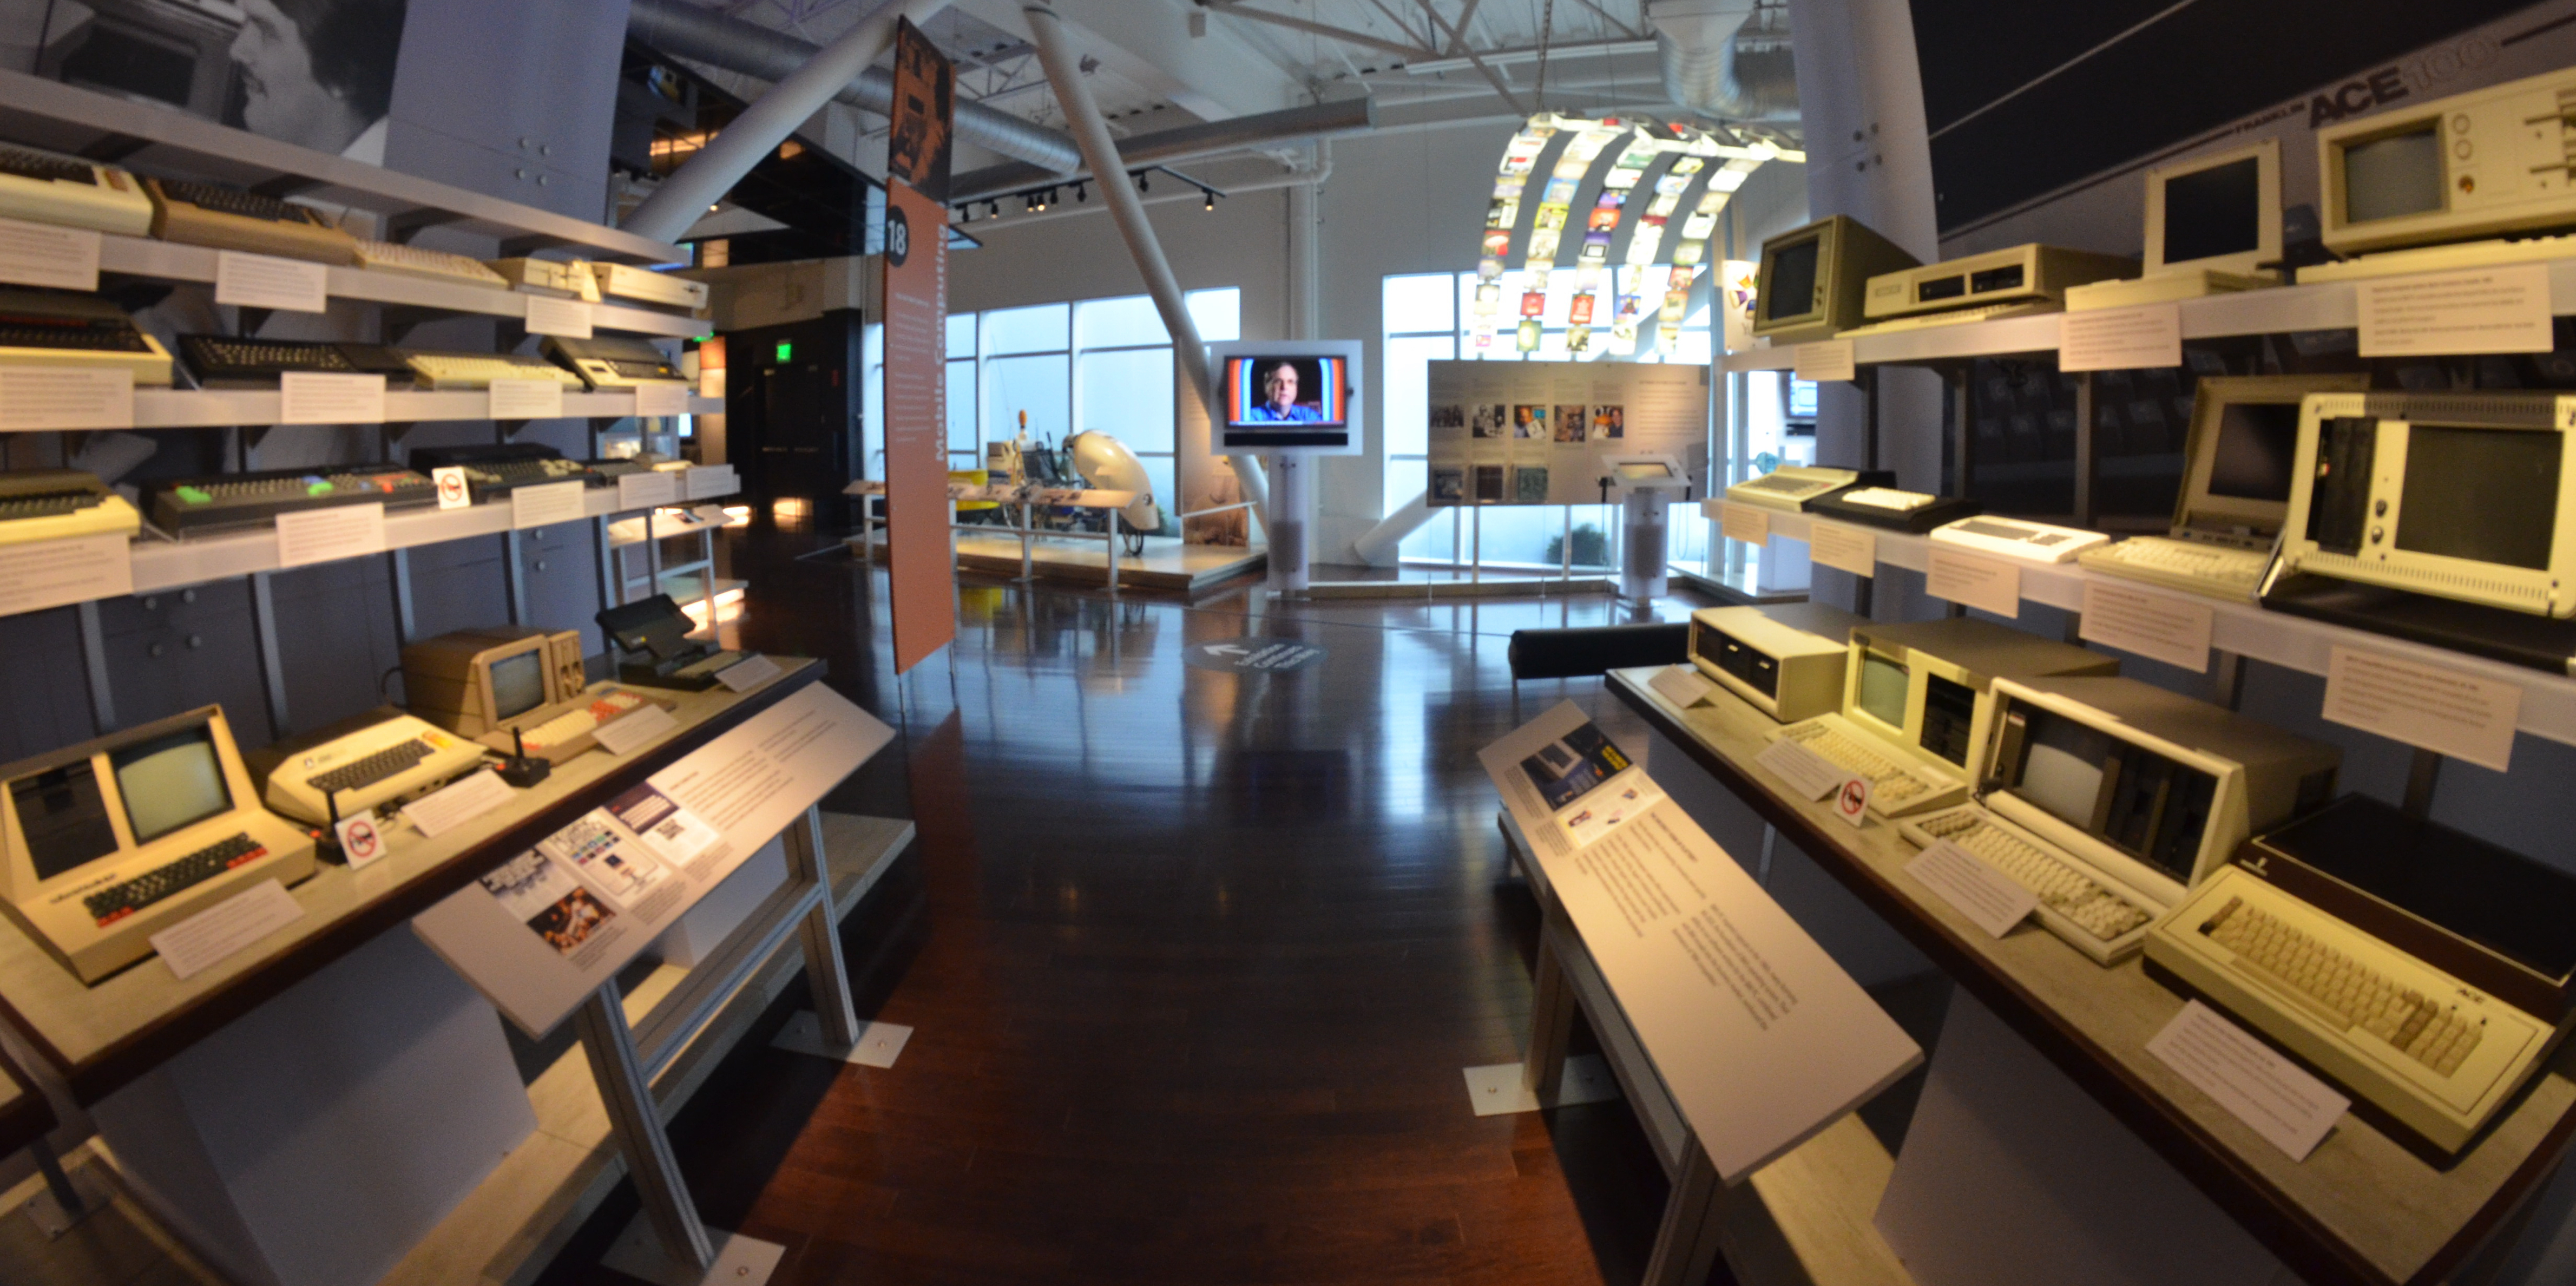
\includegraphics[width=\paperwidth]{cover}};
    \draw (current page.center) node [fill=primary, text=white, text opacity=1,inner sep=1cm]{\centering\bfseries\sffamily\parbox[c][][t]{\paperwidth}{\centering
    {\Large \@institution}\\[3pt] % Institution
    {\Huge \@title}\\[25pt] % Book title
    {\huge \@subtitle}\\[15pt] % Subtitle
    {\Large por \@author}\\[20pt] % Author
    {\large Ver. \@version \quad (\@date)}}}; % Version and date
    \end{tikzpicture}
    \vfill
    \endgroup
}
\makeatother

% Part text styling
\titlecontents{part}[0cm]
{\addvspace{20pt}\centering\large\bfseries}
{}
{}
{}

% Chapter text styling
\titlecontents{chapter}[1.25cm] % Indentation
{\addvspace{12pt}\large\sffamily\bfseries} % Spacing and font options for chapters
{\color{primary!60}\contentslabel[\Large\thecontentslabel]{1.25cm}\color{primary}} % Chapter number
{\color{primary}}
{\color{primary!60}\normalsize\;\titlerule*[.5pc]{.}\;\thecontentspage} % Page number

% Section text styling
\titlecontents{section}[1.25cm] % Indentation
{\addvspace{3pt}\sffamily\bfseries} % Spacing and font options for sections
{\contentslabel[\thecontentslabel]{1.25cm}} % Section number
{}
{\hfill\color{black}\thecontentspage} % Page number
[]

% Subsection text styling
\titlecontents{subsection}[1.25cm] % Indentation
{\addvspace{1pt}\sffamily\small} % Spacing and font options for subsections
{\contentslabel[\thecontentslabel]{1.25cm}} % Subsection number
{}
{\ \titlerule*[.5pc]{.}\;\thecontentspage} % Page number
[]

% List of figures
\titlecontents{figure}[0em]
{\addvspace{-5pt}\sffamily}
{\thecontentslabel\hspace*{1em}}
{}
{\ \titlerule*[.5pc]{.}\;\thecontentspage}
[]

% List of tables
\titlecontents{table}[0em]
{\addvspace{-5pt}\sffamily}
{\thecontentslabel\hspace*{1em}}
{}
{\ \titlerule*[.5pc]{.}\;\thecontentspage}
[]

%----------------------------------------------------------------------------------------
%	MINI TABLE OF CONTENTS IN PART HEADS
%----------------------------------------------------------------------------------------

% Chapter text styling
\titlecontents{lchapter}[0em] % Indenting
{\addvspace{15pt}\large\sffamily\bfseries} % Spacing and font options for chapters
{\color{primary}\contentslabel[\Large\thecontentslabel]{1.25cm}\color{primary}} % Chapter number
{}
{\color{primary}\normalsize\sffamily\bfseries\;\titlerule*[.5pc]{.}\;\thecontentspage} % Page number

% Section text styling
\titlecontents{lsection}[0em] % Indenting
{\sffamily\small} % Spacing and font options for sections
{\contentslabel[\thecontentslabel]{1.25cm}} % Section number
{}
{}

% Subsection text styling
\titlecontents{lsubsection}[.5em] % Indentation
{\normalfont\footnotesize\sffamily} % Font settings
{}
{}
{}

%----------------------------------------------------------------------------------------
%	PAGE HEADERS
%----------------------------------------------------------------------------------------

\usepackage{fancyhdr} % Required for header and footer configuration

\pagestyle{fancy}
\renewcommand{\chaptermark}[1]{\markboth{\sffamily\normalsize\bfseries\chaptername\ \thechapter.\ #1}{}} % Chapter text font settings
\renewcommand{\sectionmark}[1]{\markright{\sffamily\normalsize\thesection\hspace{5pt}#1}{}} % Section text font settings
\fancyhf{} \fancyhead[LE,RO]{\sffamily\normalsize\thepage} % Font setting for the page number in the header
\fancyhead[LO]{\rightmark} % Print the nearest section name on the left side of odd pages
\fancyhead[RE]{\leftmark} % Print the current chapter name on the right side of even pages
\renewcommand{\headrulewidth}{0.5pt} % Width of the rule under the header
\addtolength{\headheight}{2.5pt} % Increase the spacing around the header slightly
\renewcommand{\footrulewidth}{0pt} % Removes the rule in the footer
\fancypagestyle{plain}{\fancyhead{}\renewcommand{\headrulewidth}{0pt}} % Style for when a plain pagestyle is specified

% Removes the header from odd empty pages at the end of chapters
\makeatletter
\renewcommand{\cleardoublepage}{
\clearpage\ifodd\c@page\else
\hbox{}
\vspace*{\fill}
\thispagestyle{empty}
\newpage
\fi}

%----------------------------------------------------------------------------------------
%	THEOREM STYLES
%----------------------------------------------------------------------------------------

\usepackage{amsmath,amsfonts,amssymb,amsthm} % For math equations, theorems, symbols, etc

\newcommand{\intoo}[2]{\mathopen{]}#1\,;#2\mathclose{[}}
\newcommand{\ud}{\mathop{\mathrm{{}d}}\mathopen{}}
\newcommand{\intff}[2]{\mathopen{[}#1\,;#2\mathclose{]}}
\newtheorem{notation}{Notación}[chapter]

% Boxed/framed environments
\newtheoremstyle{primarynumbox}% % Theorem style name
{0pt}% Space above
{0pt}% Space below
{\normalfont}% % Body font
{}% Indent amount
{\small\bf\sffamily\color{primary}}% % Theorem head font
{\;}% Punctuation after theorem head
{0.25em}% Space after theorem head
{\small\sffamily\color{primary}\thmname{#1}\nobreakspace\thmnumber{\@ifnotempty{#1}{}\@upn{#2}}% Theorem text (e.g. Theorem 2.1)
\thmnote{\nobreakspace\the\thm@notefont\sffamily\bfseries\color{black}---\nobreakspace#3.}} % Optional theorem note
\renewcommand{\qedsymbol}{$\blacksquare$}% Optional qed square

\newtheoremstyle{blacknumex}% Theorem style name
{5pt}% Space above
{5pt}% Space below
{\normalfont}% Body font
{} % Indent amount
{\small\bf\sffamily}% Theorem head font
{\;}% Punctuation after theorem head
{0.25em}% Space after theorem head
{\small\sffamily{\tiny\ensuremath{\textcolor{primary}{\blacksquare}}}\nobreakspace\thmname{#1}\nobreakspace\thmnumber{\@ifnotempty{#1}{}\@upn{#2}}\\% Theorem text (e.g. Theorem 2.1)
\thmnote{\nobreakspace\the\thm@notefont\sffamily\bfseries---\nobreakspace#3.}}% Optional theorem note

\newtheoremstyle{blacknumbox} % Theorem style name
{0pt}% Space above
{0pt}% Space below
{\normalfont}% Body font
{}% Indent amount
{\small\bf\sffamily}% Theorem head font
{\;}% Punctuation after theorem head
{0.25em}% Space after theorem head
{\small\sffamily\thmname{#1}\nobreakspace\thmnumber{\@ifnotempty{#1}{}\@upn{#2}}% Theorem text (e.g. Theorem 2.1)
\thmnote{\nobreakspace\the\thm@notefont\sffamily\bfseries---\nobreakspace#3.}}% Optional theorem note

% Non-boxed/non-framed environments
\newtheoremstyle{primarynum}% % Theorem style name
{5pt}% Space above
{5pt}% Space below
{\normalfont}% % Body font
{}% Indent amount
{\small\bf\sffamily\color{primary}}% % Theorem head font
{\;}% Punctuation after theorem head
{0.25em}% Space after theorem head
{\small\sffamily\color{primary}\thmname{#1}\nobreakspace\thmnumber{\@ifnotempty{#1}{}\@upn{#2}}% Theorem text (e.g. Theorem 2.1)
\thmnote{\nobreakspace\the\thm@notefont\sffamily\bfseries\color{black}---\nobreakspace#3.}} % Optional theorem note
\renewcommand{\qedsymbol}{$\blacksquare$}% Optional qed square
\makeatother

% Defines the theorem text style for each type of theorem to one of the three styles above
\newcounter{dummy}
\numberwithin{dummy}{section}
\theoremstyle{primarynumbox}
\newtheorem{theoremeT}[dummy]{Teorema}
\newtheorem{problem}{Problema}[chapter]
\newtheorem{exerciseT}{Ejercicio}[chapter]
\theoremstyle{blacknumex}
\newtheorem{exampleT}{Ejemplo}[chapter]
\theoremstyle{blacknumbox}
\newtheorem{vocabulary}{Vocabulario}[chapter]
\newtheorem{definitionT}{Definición}[chapter]
\newtheorem{corollaryT}[dummy]{Corolario}
\theoremstyle{primarynum}
\newtheorem{proposition}[dummy]{Proposición}

%----------------------------------------------------------------------------------------
%	DEFINITION OF COLORED BOXES
%----------------------------------------------------------------------------------------

\RequirePackage[framemethod=default]{mdframed} % Required for creating the theorem, definition, exercise and corollary boxes

% Theorem box
\newmdenv[skipabove=7pt,
skipbelow=7pt,
backgroundcolor=black!5,
linecolor=primary,
innerleftmargin=5pt,
innerrightmargin=5pt,
innertopmargin=5pt,
leftmargin=0cm,
rightmargin=0cm,
innerbottommargin=5pt]{tBox}

% Exercise box
\newmdenv[skipabove=5pt,
skipbelow=7pt,
rightline=false,
leftline=true,
topline=false,
bottomline=false,
backgroundcolor=primary!10,
linecolor=primary,
innerleftmargin=5pt,
innerrightmargin=5pt,
innertopmargin=10pt,
innerbottommargin=5pt,
leftmargin=0cm,
rightmargin=0cm,
linewidth=4pt]{eBox}

% Definition box
\newmdenv[skipabove=17pt,
skipbelow=7pt,
rightline=false,
leftline=true,
topline=false,
bottomline=false,
linecolor=primary,
innerleftmargin=5pt,
innerrightmargin=5pt,
innertopmargin=10pt,
innerbottommargin=5pt,
leftmargin=0cm,
rightmargin=0cm,
linewidth=4pt]{dBox}

% Corollary box
\newmdenv[skipabove=7pt,
skipbelow=7pt,
rightline=false,
leftline=true,
topline=false,
bottomline=false,
linecolor=gray,
backgroundcolor=black!5,
innerleftmargin=5pt,
innerrightmargin=5pt,
innertopmargin=5pt,
leftmargin=0cm,
rightmargin=0cm,
linewidth=4pt,
innerbottommargin=5pt]{cBox}

% Creates an environment for each type of theorem and assigns it a theorem text style from the "Theorem Styles" section above and a colored box from above
\newenvironment{theorem}{\begin{tBox}\begin{theoremeT}}{\end{theoremeT}\end{tBox}}
\newenvironment{exercise}{\begin{eBox}\begin{exerciseT}}{\hfill{\color{primary}\tiny\ensuremath{\blacksquare}}\end{exerciseT}\end{eBox}}
\newenvironment{knowwhat}[1][Sabías qué]{\begin{eBox}\textcolor{primary}{\textbf{#1}}\\}{\hfill{\color{primary}}\end{eBox}}
\newenvironment{definition}{\begin{dBox}\begin{definitionT}}{\end{definitionT}\end{dBox}}
\newenvironment{example}{\begin{exampleT}}{\hfill{\tiny\ensuremath{\blacksquare}}\end{exampleT}}
\newenvironment{corollary}{\begin{cBox}\begin{corollaryT}}{\end{corollaryT}\end{cBox}}
\newenvironment{solution}{\vspace*{10pt}}{\vspace*{30pt}}

%----------------------------------------------------------------------------------------
%	REMARK ENVIRONMENT
%----------------------------------------------------------------------------------------

\newenvironment{remark}{\par\vspace{10pt}\small % Vertical white space above the remark and smaller font size
\begin{list}{}{
\leftmargin=35pt % Indentation on the left
\rightmargin=25pt}\item\ignorespaces % Indentation on the right
\makebox[-2.5pt]{\begin{tikzpicture}[overlay]
\node[draw=primary!60,line width=1pt,circle,fill=primary!25,font=\sffamily\bfseries,inner sep=2pt,outer sep=0pt] at (-15pt,0pt){\textcolor{primary}{!}};\end{tikzpicture}} % Orange R in a circle
\advance\baselineskip -1pt}{\end{list}\vskip5pt} % Tighter line spacing and white space after remark

\newenvironment{hint}{\par\vspace{10pt}\small % Vertical white space above the remark and smaller font size
\begin{list}{}{
\leftmargin=35pt % Indentation on the left
\rightmargin=25pt}\item\ignorespaces % Indentation on the right
\makebox[-2.5pt]{\begin{tikzpicture}[overlay]
\node[draw=yellow!60,line width=1pt,circle,fill=yellow!25,font=\sffamily\bfseries,inner sep=2pt,outer sep=0pt] at (-15pt,0pt){\textcolor{yellow}{X}};\end{tikzpicture}} % Orange R in a circle
\advance\baselineskip -1pt}{\end{list}\vskip5pt} % Tighter line spacing and white space after remark

\newenvironment{question}{\par\vspace{10pt}\small % Vertical white space above the remark and smaller font size
\begin{list}{}{
\leftmargin=35pt % Indentation on the left
\rightmargin=25pt}\item\ignorespaces % Indentation on the right
\makebox[-2.5pt]{\begin{tikzpicture}[overlay]
\node[draw=blue!60,line width=1pt,circle,fill=blue!25,font=\sffamily\bfseries,inner sep=2pt,outer sep=0pt] at (-15pt,0pt){\textcolor{blue}{?}};\end{tikzpicture}} % Orange R in a circle
\advance\baselineskip -1pt}{\end{list}\vskip5pt} % Tighter line spacing and white space after remark

\newenvironment{money}{\par\vspace{10pt}\small % Vertical white space above the remark and smaller font size
\begin{list}{}{
\leftmargin=35pt % Indentation on the left
\rightmargin=25pt}\item\ignorespaces % Indentation on the right
\makebox[-2.5pt]{\begin{tikzpicture}[overlay]
\node[draw=green!60,line width=1pt,circle,fill=green!25,font=\sffamily\bfseries,inner sep=2pt,outer sep=0pt] at (-15pt,0pt){\textcolor{green}{\$}};\end{tikzpicture}} % Orange R in a circle
\advance\baselineskip -1pt}{\end{list}\vskip5pt} % Tighter line spacing and white space after remark


%----------------------------------------------------------------------------------------
%	SECTION NUMBERING IN THE MARGIN
%----------------------------------------------------------------------------------------

\makeatletter
\renewcommand{\@seccntformat}[1]{\llap{\textcolor{primary}{\csname the#1\endcsname}\hspace{1em}}}
\renewcommand{\section}{\@startsection{section}{1}{\z@}
{-4ex \@plus -1ex \@minus -.4ex}
{1ex \@plus.2ex }
{\normalfont\large\sffamily\bfseries}}
\renewcommand{\subsection}{\@startsection {subsection}{2}{\z@}
{-3ex \@plus -0.1ex \@minus -.4ex}
{0.5ex \@plus.2ex }
{\normalfont\sffamily\bfseries}}
\renewcommand{\subsubsection}{\@startsection {subsubsection}{3}{\z@}
{-2ex \@plus -0.1ex \@minus -.2ex}
{.2ex \@plus.2ex }
{\normalfont\small\sffamily\bfseries}}
\renewcommand\paragraph{\@startsection{paragraph}{4}{\z@}
{-2ex \@plus-.2ex \@minus .2ex}
{.1ex}
{\normalfont\small\sffamily\bfseries}}

%----------------------------------------------------------------------------------------
%	PART HEADINGS
%----------------------------------------------------------------------------------------

% numbered part in the table of contents
\newcommand{\@mypartnumtocformat}[2]{%
\setlength\fboxsep{0pt}%
\noindent\colorbox{primary!20}{\strut\parbox[c][.7cm]{\ecart}{\color{primary!70}\Large\sffamily\bfseries\centering#1}}\hskip\esp\colorbox{primary!40}{\strut\parbox[c][.7cm]{\linewidth-\ecart-\esp}{\Large\sffamily\centering#2}}}%
%%%%%%%%%%%%%%%%%%%%%%%%%%%%%%%%%%
% unnumbered part in the table of contents
\newcommand{\@myparttocformat}[1]{%
\setlength\fboxsep{0pt}%
\noindent\colorbox{primary!40}{\strut\parbox[c][.7cm]{\linewidth}{\Large\sffamily\centering#1}}}%
%%%%%%%%%%%%%%%%%%%%%%%%%%%%%%%%%%
\newlength\esp
\setlength\esp{4pt}
\newlength\ecart
\setlength\ecart{1.2cm-\esp}
\newcommand{\thepartimage}{}%
\newcommand{\partimage}[1]{\renewcommand{\thepartimage}{#1}}%
\def\@part[#1]#2{%
\ifnum \c@secnumdepth >-2\relax%
\refstepcounter{part}%
\addcontentsline{toc}{part}{\texorpdfstring{\protect\@mypartnumtocformat{\thepart}{#1}}{\partname~\thepart\ ---\ #1}}
\else%
\addcontentsline{toc}{part}{\texorpdfstring{\protect\@myparttocformat{#1}}{#1}}%
\fi%
\startcontents%
\markboth{}{}%
{\thispagestyle{empty}%
\begin{tikzpicture}[remember picture,overlay]%
\node at (current page.north west){\begin{tikzpicture}[remember picture,overlay]%
\fill[primary!20](0cm,0cm) rectangle (\paperwidth,-\paperheight);
\node[anchor=north] at (4cm,-3.25cm){\color{primary!40}\fontsize{220}{100}\sffamily\bfseries\thepart};
\node[anchor=south east] at (\paperwidth-1cm,-\paperheight+1cm){\parbox[t][][t]{8.5cm}{
\printcontents{l}{0}{\setcounter{tocdepth}{1}}%
}};
\node[anchor=north east] at (\paperwidth-1.5cm,-3.25cm){\parbox[t][][t]{15cm}{\strut\raggedleft\color{white}\fontsize{30}{30}\sffamily\bfseries#2}};
\end{tikzpicture}};
\end{tikzpicture}}%
\@endpart}
\def\@spart#1{%
\startcontents%
\phantomsection
{\thispagestyle{empty}%
\begin{tikzpicture}[remember picture,overlay]%
\node at (current page.north west){\begin{tikzpicture}[remember picture,overlay]%
\fill[primary!20](0cm,0cm) rectangle (\paperwidth,-\paperheight);
\node[anchor=north east] at (\paperwidth-1.5cm,-3.25cm){\parbox[t][][t]{15cm}{\strut\raggedleft\color{white}\fontsize{30}{30}\sffamily\bfseries#1}};
\end{tikzpicture}};
\end{tikzpicture}}
\addcontentsline{toc}{part}{\texorpdfstring{%
\setlength\fboxsep{0pt}%
\noindent\protect\colorbox{primary!40}{\strut\protect\parbox[c][.7cm]{\linewidth}{\Large\sffamily\protect\centering #1\quad\mbox{}}}}{#1}}%
\@endpart}
\def\@endpart{\vfil\newpage
\if@twoside
\if@openright
\null
\thispagestyle{empty}%
\newpage
\fi
\fi
\if@tempswa
\twocolumn
\fi}

%----------------------------------------------------------------------------------------
%	CHAPTER HEADINGS
%----------------------------------------------------------------------------------------

% A switch to conditionally include a picture, implemented by  Christian Hupfer
\newif\ifusechapterimage
\usechapterimagetrue
\newcommand{\thechapterimage}{}%
\newcommand{\thechapterimagedescription}{}%
\newcommand{\thechapterimageauthor}{}%
\newcommand{\chapterimage}[1]{\ifusechapterimage\renewcommand{\thechapterimage}{#1}\fi}%
\newcommand{\chapterimagedescription}[1]{\ifusechapterimage\renewcommand{\thechapterimagedescription}{#1}\fi}%
\newcommand{\chapterimageauthor}[1]{\ifusechapterimage\renewcommand{\thechapterimageauthor}{#1}\fi}%
\newcommand{\autodot}{.}
\def\@makechapterhead#1{%
{\parindent \z@ \raggedright \normalfont
\ifnum \c@secnumdepth >\m@ne
\if@mainmatter
\begin{tikzpicture}[remember picture,overlay]
\node at (current page.north west)
{\begin{tikzpicture}[remember picture,overlay]
\node[anchor=north west,inner sep=0pt] at (0,0) {\ifusechapterimage\includegraphics[width=\paperwidth]{\thechapterimage}\fi};
\draw[anchor=west] (\Gm@lmargin,-9cm) node [line width=2pt,rounded corners=15pt,draw=primary,fill=white,fill opacity=0.5,inner sep=15pt]{\strut\makebox[22cm]{}};
\draw[anchor=west] (\Gm@lmargin+.3cm,-9cm) node {\huge\sffamily\bfseries\color{black}\thechapter\autodot~#1\strut};
\draw[anchor=east] (\Gm@lmargin+17.5cm,-11.5cm) node {\ifusechapterimage{\raggedright\color{gray}\thechapterimagedescription\autodot}\fi};
\draw[anchor=east] (\Gm@lmargin+17.5cm,-12cm) node {\ifusechapterimage{\raggedright\color{gray}\thechapterimageauthor\autodot}\fi};
\end{tikzpicture}};
\end{tikzpicture}
\else
\begin{tikzpicture}[remember picture,overlay]
\node at (current page.north west)
{\begin{tikzpicture}[remember picture,overlay]
\node[anchor=north west,inner sep=0pt] at (0,0) {\ifusechapterimage\includegraphics[width=\paperwidth]{\thechapterimage}\fi};
\draw[anchor=west] (\Gm@lmargin,-9cm) node [line width=2pt,rounded corners=15pt,draw=primary,fill=white,fill opacity=0.5,inner sep=15pt]{\strut\makebox[22cm]{}};
\draw[anchor=west] (\Gm@lmargin+.3cm,-9cm) node {\huge\sffamily\bfseries\color{black}#1\strut};
%\draw[anchor=east] (\Gm@lmargin+17.5cm,-11cm) node {\ifusechapterimage{\raggedright\color{gray}\thechapterimagedescription\autodot}\fi};
%\draw[anchor=east] (\Gm@lmargin+17.5cm,-11.5cm) node {\ifusechapterimage{\raggedright\color{gray}\thechapterimageauthor\autodot}\fi};
\end{tikzpicture}};
\end{tikzpicture}
\fi\fi\par\vspace*{270\p@}}}

%-------------------------------------------

\def\@makeschapterhead#1{%
\begin{tikzpicture}[remember picture,overlay]
\node at (current page.north west)
{\begin{tikzpicture}[remember picture,overlay]
\node[anchor=north west,inner sep=0pt] at (0,0) {\ifusechapterimage\includegraphics[width=\paperwidth]{\thechapterimage}\fi};
\draw[anchor=west] (\Gm@lmargin,-9cm) node [line width=2pt,rounded corners=15pt,draw=primary,fill=white,fill opacity=0.5,inner sep=15pt]{\strut\makebox[22cm]{}};
\draw[anchor=west] (\Gm@lmargin+.3cm,-9cm) node {\huge\sffamily\bfseries\color{black}#1\strut};
\draw[anchor=east] (\Gm@lmargin+17.5cm,-11.5cm) node {\ifusechapterimage{\raggedright\color{gray}\thechapterimagedescription\autodot}\fi};
\draw[anchor=east] (\Gm@lmargin+17.5cm,-12cm) node {\ifusechapterimage{\raggedright\color{gray}\thechapterimageauthor\autodot}\fi};
\end{tikzpicture}};
\end{tikzpicture}
\par\vspace*{270\p@}}
\makeatother

%----------------------------------------------------------------------------------------
%	HYPERLINKS IN THE DOCUMENTS
%----------------------------------------------------------------------------------------

\usepackage{hyperref}
\hypersetup{hidelinks,backref=true,pagebackref=true,hyperindex=true,colorlinks=false,breaklinks=true,urlcolor= primary,bookmarks=true,bookmarksopen=false,pdftitle={Title},pdfauthor={Author}}
\usepackage{bookmark}
\bookmarksetup{
open,
numbered,
addtohook={%
\ifnum\bookmarkget{level}=0 % chapter
\bookmarksetup{bold}%
\fi
\ifnum\bookmarkget{level}=-1 % part
\bookmarksetup{color=primary,bold}%
\fi
}
}

%----------------------------------------------------------------------------------------
%	SPECIAL TRANSLATIONS
%----------------------------------------------------------------------------------------
\addto\extrasspanish{%
\def\partautorefname{Unidad}%
\def\appendixautorefname{Anexo}%
}

%----------------------------------------------------------------------------------------
%	SPECIAL INDENTS AND LINES
%----------------------------------------------------------------------------------------
\newcommand{\crline}[2][10pt]{
    \noindent #2

    \vspace{#1}
}

\newcounter{sindentwidth}
\newcounter{dindentwidth}
\setcounter{sindentwidth}{16}
\setcounter{dindentwidth}{32}

\newcommand{\sindent}{\noindent\hspace*{\value{sindentwidth} pt}}
\newcommand{\dindent}{\noindent\hspace*{\value{dindentwidth} pt}}

%----------------------------------------------------------------------------------------
%	EMOJI IMAGES SUPPORT (IMAGES NOT PROVIDED)
%----------------------------------------------------------------------------------------
\newcommand{\emoji}[1]{%
  \includegraphics[width=1em,valign=t,raise=-0.1em]{#1}%
}

%----------------------------------------------------------------------------------------
%	DARK MODE SUPPORT
%----------------------------------------------------------------------------------------
\newcommand{\darkmode}{
  \pagecolor{black!80}
  \color{white!30}
}
 % Insert the thebook.tex file which contains the majority of the structure behind the template

\addbibresource{bibliography.bib}

\begin{document}

%----------------------------------------------------------------------------------------
%	DOCUMENT CONFIGURATION
%----------------------------------------------------------------------------------------

\title{Elementos de Programación y Lógica}
\subtitle{Cuadernillo del estudiante}
\department{Departamento de Ciencia y Tecnología}
\institution{Universidad Nacional de Quilmes}
\author{Alan Rodas Bonjour}
\version{0.4}
\date{17/03/2019}

\primarycolor{176}{30}{45}

\maketitle

\newpage
~\vfill
\thispagestyle{empty}

\crline{Copyright \copyright\ 2019 Alan Rodas Bonjour} % Copyright notice

\crline{\textsc{Publicado online por Alan Rodas Bonjour}} % Publisher

\crline[25pt]{\textsc{http://elementosdeprogramacionylogica.web.unq.edu.ar}} % URL


\crline{\includegraphics[scale=0.5]{cc-by-nc-sa}}

\crline{Licenciado bajo los términos de la siguiente licencia de contenidos:
Licencia Creative Commons Atribución-NoComercial-CompartirIgual 4.0 Internacional
(la ``licencia''). Puede obtener una copia completa de ella en
\url{https://creativecommons.org/licenses/by-nc-sa/4.0/deed.es}.}

\crline{
    Usted tiene derecho a:
    \begin{itemize}
        \item \textbf{Compartir}: copiar y redistribuir el material en cualquier
        medio o formato
        \item \textbf{Adaptar}: remezclar, transformar y construir a partir del
        material
    \end{itemize}
}

\crline{El licenciante no puede revocar estas libertades en tanto usted siga los
términos siguientes.}

\crline{
    \begin{itemize}
        \item \textbf{Atribución}: Usted debe dar crédito de manera adecuada,
        brindar un enlace a la licencia, e indicar si se han realizado cambios.
        Puede hacerlo en cualquier forma razonable, pero no de forma tal que
        sugiera que usted o su uso tienen el apoyo de la licenciante.
        \item \textbf{NoComercial}: Usted no puede hacer uso del material con
        propósitos comerciales.
        \item \textbf{CompartirIgual}: Si remezcla, transforma o crea a partir
        del material, debe distribuir su contribución bajo la la misma licencia
        del original.
    \end{itemize}
}

\crline{No hay restricciones adicionales — No puede aplicar términos legales ni
medidas tecnológicas que restrinjan legalmente a otras a hacer cualquier uso
permitido por la licencia.}

\crline{No tiene que cumplir con la licencia para elementos del material en el
dominio público o cuando su uso esté permitido por una excepción o limitación
aplicable.}

\crline{No se dan garantías. La licencia podría no darle todos los permisos que
 necesita para el uso que tenga previsto. Por ejemplo, otros derechos como
 publicidad, privacidad, o derechos morales pueden limitar la forma en que
 utilice el material.}

% License information

\crline{\textit{Primera edición, Febrero 2019}} % Printing/edition date


\chapterimage{indice}
\pagestyle{empty}
\tableofcontents
\cleardoublepage
\pagestyle{fancy}

\setlength{\parskip}{0.5em}

\chapterimage{imagenes/introduccion.jpg}
\chapterimagedescription{Imagen de la supercomputadora Thunderbird, en el Sandia National Laboratory.}
\chapterimageauthor{Fotografía del Departamento de Energía de los Estados Unidos}

\chapter*{Introducción}

La \textbf{informática} es la disciplina o campo de estudio que abarca el
\textbf{conjunto de conocimientos, métodos y técnicas referentes al tratamiento
automático de la información, junto con sus teorías y aplicaciones prácticas,
con el fin de almacenar, procesar y transmitir datos e información en formato
digital utilizando sistemas computacionales}. Los datos son la materia prima
para que, mediante su proceso, se obtenga como resultado información. Para ello,
la  informática crea y/o emplea sistemas de procesamiento de datos, que incluyen
medios físicos en interacción con medios lógicos y las personas que los
programan y los usan.

\section*{Temas a tratar}

Como este campo requiere el uso de \textbf{computadoras} (en el sentido amplio
de la palabra), comenzaremos en la unidad \ref{Computadoras} por analizar qué es
una computadora, ver como funcionan, de que partes están compuestas y una breve
historia de las mismas. Se debe tener en cuenta que nos centraremos en
computadoras electrónicas, también llamadas clásicas, las cuales son las que
predominan en el mercado. Sin embargo, analizaremos otras variantes de
computadoras cuando veamos la historia de las mismas, como las computadoras
mecánicas. Así mismo, los conceptos teóricos que rigen las ciencias de la
computación, auguran como posibilidades otros modelos computacionales, todavía
en etapas muy inmaduras, como las computadoras cuánticas, o las biológicas,
tema que tocaremos brevemente.

En la unidad \ref{Información} analizaremos como las computadoras almacenan
\textbf{información}, y como se procesa y se interpreta la misma. Haremos una
mínima introducción a lo que es el concepto de datos binarios, y veremos como
con ese sistema se almacenan números, letras, colores, imágenes, videos y
cualquier información que uno desee. Veremos como funcionan los editores de
texto y los visualizadores de archivos, y tendremos un primer acercamiento a
un lenguaje informático mediante el uso de lenguajes de marcado. Evitaremos
mencionar los estándares que rigen las computadoras modernas, pues solamente nos
interesará el concepto subyacente a los mismos, por lo que algunos lectores que
posean conocimiento de esta temática podrán sentir que se ha tomado una
aproximación muy laxa. Tenga en cuenta el lector que la omisión es intencional.

Posteriormente en la unidad \ref{Lógica} analizaremos la \textbf{lógica}, uno los
fundamentos teóricos más importantes que subyace en la disciplina. Analizaremos
parte de los formalismos que rigen en esta ciencia y veremos como se aplican
esos conceptos en matemática y en ciencias de la computación en general. El foco
del presente no es realizar un análisis exhaustivo de esta disciplina, la cual
es sumamente amplia para abarcarla en tan pocas páginas. Aparecerán entonces
los conceptos de conectivas, y las utilizaremos para formular preguntas nuevas a
partir de otras que ya teníamos disponibles, un concepto muy útil a la hora
de programar. También hablaremos de razonamientos deductivos, de sus premisas y
conclusión, y aplicaremos los conocimientos de forma práctica para introducirnos
en la lógica proposicional y descubrir sus formalismos. Finalmente, veremos
razonamientos que no pueden resolverse con la lógica proposicional y mojaremos
nuestros pies en la superficie de la lógica de predicados, analizando muy brevemente
sus formalismos.

Por último, en la unidad \ref{Programación} veremos como se procesa información utilizando
\textbf{programación}. Crearemos nuestros primeros programas que solucionarán
pequeños problemas, y analizaremos los mismos para descubrir algunas de las
estructuras más comúnmente utilizadas en programación. Nuevamente, la disciplina
es amplia, y por tanto solo abordaremos pequeñas cuestiones puntuales, como la
secuencia de comandos para generar programas, el uso de estructuras de control
para estructurar ideas y reducir la cantidad de código, así como generar
soluciones más genéricas. Por sobre todo trabajaremos en planificar nuestras
soluciones en forma de tareas pequeñas para simplificar la complejidad del
problema a resolver, así como comunicar correcta y eficazmente nuestra solución.
Los lectores que tengan conocimientos previos en esta área sentirán al comienzo
que lo presentado es muy básico, y que aporta poco a su saber. Sin embargo,
recomendamos no tomarse a la ligera lo presentado en esta unidad, pues el
abordaje elegido difiere del seleccionado por muchos autores, y hace especial
hincapié en la comunicación de la solución al problema, concepto fundamental
para convertirse en un programador profesional.

\section*{Estructura del libro}

El presente se estructura entonces en cuatro unidades y una unidad adicional
que contiene el índice y una serie de anexos. Cada unidad a su vez, se
divide en capítulos, y cada capítulo en diferentes secciones.

Cada capítulo del presente se apoya en lo visto en capítulos anteriores, y si
bien pueden leerse de forma independiente, esto trae aparejado el supuesto de
ciertos conocimientos ya vistos, por lo que recomendamos leer el libro de
forma completa y continuada.

El texto intenta ser lo más breve y directo posible, para permitir la comprensión
incluso a los menos asiduos a la lectura. Por otro lado, se intenta explicar los
conceptos con definiciones más pragmáticas que enciclopédicas. Si bien esto puede
no ser del agrado de todos los lectores, creemos que la comprensión del concepto
es más importante que una definición, la cual en general varía de autor en autor.
Si bien en algunos lugares se sacrifica precisión en pos de la comprensión, en
todo lugar donde esto ocurre es deliberado, pues no se desea sobrecargar el libro
en conceptos que, si bien importantes para un profesional de la industria, no
son relevantes para quien busca adquirir conocimientos generales de la temática.

Al final de cada capítulo se presentan ejercicios prácticos a realizar, los
cuales tienen dos propósitos. Por un lado, muchos de ellos sirven para asentar
los conocimientos teóricos vistos utilizando un enfoque práctico. Por otro,
algunos de ellos ocultan detalles teóricos interesantes que no pudieron entrar
en estas páginas por motivos de espacio.

Los ejercicios suelen tomar unos pocos minutos en resolverse, dado que el lector
haya comprendido correctamente todos los temas de la unidad, y recomendamos
que se vayan realizando a medida que se avanza con la lectura. 

Al final de cada unidad se presenta un conjunto de bibliografía adicional que
permitirá al lector expandir sus conocimientos o abordar con mayor profundidad
en las diversas temáticas abordadas aquí, así como también tener otros puntos de
vista.

La última parte del libro contiene el índice con las palabras clave, y los lugares
en donde dichas palabras aparecen en el libro de forma relevante. También
posee una serie de anexos, los cuales presentan información adicional sobre
una temática particular, o resultan útiles de tener a mano a la hora de realizar
las actividades propuestas.

\section*{Requisitos y saberes previos}

Para poder comprender los contenidos de este libro no se requieren demasiados
saberes previos. Se espera sin embargo, que el lector posea algunos conceptos
básicos de matemática, que incluyen aritmética elemental y algo de geometría.

También se espera que el lector sepa utilizar una computadora, o se haya cruzado
en algún momento con una. Si bien existen diversos tipos de computadora, y
diversas formas de interactuar con las mismas, el presente toma por supuesto
que el lector ha utilizado una computadora de escritorio o notebook, y que sabe
lo que es un teléfono móvil inteligente (smartphone), haya o no interactuado con
uno.

La unidad \ref{Lógica}, en su última sección, se vuelve más sencilla de
comprender si el lector se cruzó previamente con el concepto de función
(en términos de análisis matemático), aunque no es imprescindible para la
correcta comprensión de los temas abordados.

Para seguir la teoría de la unidad \ref{Programación}, así como resolver los
ejercicios propuestos puede recurrir solamente a la lectura, lápiz y papel. Sin
embargo, realizar los ejercicios en la computadora facilitará una mayor
comprensión de los conceptos, simplificando el proceso de aprendizaje. Para esto
se espera que lector cuente con acceso a una computadora, ya sea una notebook o
máquina de escritorio, y acceso a internet (ya sea continuo o esporádico).

\section*{Comentarios finales}

La disciplina de las ciencias de la computación y la informática en general
son campos relativamente nuevos (aunque sus orígenes datan de más de tres
milenios atrás, no se comenzó a considerar la informática como una ciencia en
si misma sino hasta comienzos del siglo XX). Aún así, esta disciplina ha
evolucionado mucho en un muy corto período de tiempo, revolucionando de forma
sustancial el mundo en el que vivimos.

Si bien las computadoras son omnipresentes en nuestro día a día, todo indica
que recién estamos nadando en la superficie de las aguas de lo que es posible
con la informática, y que el futuro nos depara una inmersión en las mismas,
a profundidades que aún no alcanzamos a vislumbrar. Las posibilidades auguradas
por las ciencias de la computación son muchas y muy amplias, y es un campo en
completa expansión, que trabaja cada vez más de forma interdisciplinar con
ciencias tan dispares como la física, la biología, la neurología, la lingüística,
la economía, la política, e incluso la filosofía.

Por otro lado, como ya mencionamos, la informática tiene que ver con el proceso
y manejo de la información. Ser meros usuarios de tecnologías, desconociendo
completamente los conceptos subyacentes más básicos de los mismos, nos vuelve
vulnerables a engaños y manipulaciones por quienes controlan la información.
¿Es bueno el voto electrónico? ¿Qué datos tienen las empresas sobre mi persona
y cómo pueden utilizarlos? ¿Es seguro utilizar una tarjeta de crédito en internet?
Si conocemos los conceptos subyacentes a la tecnología que utilizamos, responder
esas preguntas se vuelve más sencillo, y nos permite tomar mejores decisiones
como ciudadanos digitales.

Muchos especialistas afirman que dentro de pocos años en el futuro, desconocer
estos conceptos será equivalente a no saber leer y escribir en la sociedad
actual. Por eso este libro apunta a brindar un panorama introductorio, pero
lo suficientemente amplio como para que el lector obtenga un panorama
general de los conceptos principales de la informática generalmente
desconocidos.

%%%%%%%%%%%%%%%%%%%%%%%%%%%%%%%%%%%%%%%%%%%%%%%%

\part{Computadoras}
\label{Computadoras}

\begin{refsection}
\chapterimage{capitulos/computadoras/imagenes/cover}
\chapterimagedescription{Placa base de una computadora con sus circuitos impresos}
\chapterimageauthor{Fotografía de Blickpixel}

\chapter{Computadoras}
\index{Computadora}

Las utilizamos todos los días, rigen nuestra vida cotidiana, y el mundo moderno
dejaría de funcionar sin ellas. Las computadoras son omnipresentes en nuestro
día a día, ya sea que trabajemos directamente con ellas o no. Pero,
¿Qué es exactamente una computadora?, y más aún ¿Pará que sirve?.

Este capítulo intenta responder todas esas interrogantes y generar un glosario
de los términos más comunes en informática. No es el fin de este capítulo
centrarnos en detalles, sino obtener un panorama general de una computadora y
como esta funciona. Capítulos siguientes retomarán este contenido y
complementarán aportando detalles más específicos.

Comencemos entonces por definir qué es una computadora:

\begin{definition}
    Una \textbf{computadora} es una máquina electrónica o electromecánica que recibe
    datos, los analiza, procesa y transforma, convirtiéndolos en información
    conveniente y útil para el posterior uso por seres humanos.\autocite[vid. p.10]{gookin_2005}
\end{definition}

\wraplimage[0.25]{capitulos/computadoras/imagenes/apple_II.jpg}
{Vieja Apple II.}
{Exhibición del Musée Bolo, Lausana, Suiza.}

Es decir, una computadora es un dispositivo cuya única función es la de procesar
datos. Esos datos, también suelen ser llamados ``información'', y podrían
ser procesados por un ser humano sin ningún problema. Lo que hace a una
computadora realmente interesante es que \textbf{es capaz de procesar gran
cantidad de datos en muy poco tiempo}. Así, una tarea que implique procesar
grandes volúmenes de información, o procesarla de formas complejas (tarea que le
podría llevar a una persona meses, o incluso años) a una computadora le puede
llevar pocos segundos.\autocite[vid. p.8]{clark_scott_2009}

Toda computadora está formada físicamente por numerosos componentes electrónicos
y electro-mecánicos. Además, toda computadora cuenta con algún dispositivo que
permite ingresar datos a la misma (por ejemplo, un teclado o un mouse), y algún
otro dispositivo que permite ver los datos que la computadora procesó (por
ejemplo, un monitor o una impresora).

Cuando se habla de computadora, generalmente pensamos en la típica
\textbf{computadora de escritorio} (con su voluminoso gabinete, un monitor,
teclado y mouse). Sin embargo, las computadoras tienen hoy en día
formas cada vez más diversas, como por ejemplo, las \textbf{notebooks}, y sus
primas pequeñas las \textbf{netbooks}. Las \textbf{tablets}, los \textbf{celulares}
e incluso los \textbf{relojes inteligentes} son también ejemplos de computadoras.
Cada una tiene sus particularidades, por ejemplo, la forma de ingresar datos en
una notebook no es la misma que en un celular. Sin embargo, todas son
computadoras y comparten características comunes.

De hecho, la definición de computadora que utilizamos es tan amplia, que abarca
una serie de dispositivos que en general no clasificaríamos como computadoras,
pero que, por sus características, lo son. Además de las anteriormente
mencionadas podríamos incluir también:

\begin{itemize}
    \item \textbf{Consolas de videojuegos}
    \item \textbf{Juguetes electrónicos}
    \item \textbf{Sistemas de domótica (IoT)}
    \item \textbf{Computadoras de abordo (en autos, barcos y aviones)}
    \item \textbf{Robots}
    \item \textbf{Calculadoras graficadoras programables}
    \item \textbf{Microcontroladores}
\end{itemize}

Muchos otros dispositivos también podrían ser consideradas computadoras, o
incluyen computadoras como un componente fundamental para poder funcionar.
\autocite[introduction]{ceruzzi_2003}

\begin{knowwhat}[En realidad]
Técnicamente cualquier dispositivo electrónico que realice cálculos (cómputos)
es una computadora. Sin embargo, en general nos referimos como computadora a
aquellos dispositivos que son ``programables'', es decir, que pueden configurarse
para llevar a cabo distintas tareas por parte del usuario. Está distinción no
nos resulta relevante.
\end{knowwhat}

Una computadora está constituida por dos partes fundamentales: El
\textbf{hardware}, que comprende a la \textbf{parte física} de una computadora,
y el \textbf{software}, es decir, la parte \textbf{parte lógica}. A continuación
trataremos más en detalle ambas partes.

\section{Hardware (parte física)}
\index{Hardware}\index{Parte Fisica@Parte Física}

Comencemos por definir a qué nos referimos cuando hablamos de hardware:

\begin{definition}
    El \textbf{hardware} comprende todos los elementos físicos que componen a la
    computadora. Es decir, el conjunto de circuitos, cables, perillas, palancas,
    botones, luces, displays, dispositivos de impresión, motores, imanes, placas
    metálicas, etc.\autocite[vid. p.12]{gookin_2005}
\end{definition}

Una definición más pragmática sería: \textbf{si no funciona y lo puedo patear,
es hardware}.

Los componentes físicos que tenga la computadora, serán dependientes del tipo de
computadora con la que contemos. Así por ejemplo, algunas tendrán un teclado,
mientras que otras contarán con una pantalla táctil; unas tendrán un monitor,
mientras otras tendrán un display indicador; etc.

Muchos de estos dispositivos trabajan con elementos que no son puramente
eléctricos, sino físicos o mecánicos. A estos se los denomina
\textbf{dispositivos analógicos}. En general, los datos que emiten o reciben
tienen forma de onda (son valores continuos sobre un rango).

Los dispositivos que no emplean partes mecánicas, sino solamente electrónicas,
suelen emitir o recibir datos discretos (valores puntuales, que no conforman
un espectro). Este tipo de dispositivos se denominan \textbf{dispositivos
digitales}.

La mayoría de las computadoras de hoy en días (aunque no siempre es así, ni
tampoco fue así siempre) contienen una serie de partes relativamente estándar
 entre las que destacan:
\begin{description}
    \item[Fuente de alimentación (Fuente de poder)]\index{Fuente de Alimentacion@Fuente de Alimentación}
        Se trata de un transformador de electricidad que modifica la corriente
        que le llega (por ejemplo, desde un enchufe en la pared, con 220V, o
        desde una batería de litio), al voltaje que requiere la máquina para
        funcionar (por ejemplo, 12V, 5V, etc.). Como las computadoras son
        aparatos electrónicos, todas requieren electricidad de alguna forma.
        Este dispositivo se encarga entonces de darle energía a todos los otros
        componentes de la máquina.
    \item[Motherboard (Placa base o tarjeta madre)]\index{Motherboard}
        Consiste en una tarjeta o placa, que contiene los circuitos principales
        de la computadora impresos en un material conductivo (cobre, oro, etc.)
        sobre su superficie. La placa cuenta con ranuras (la mayoría
        estandarizadas) en donde se conectan los diversos componentes del
        equipo (aunque a veces los mismos pueden estar soldados directamente
        a la placa). Sus circuitos se encargan de conectar y a los diversos
        componentes entre sí, permitiendo que la electricidad fluya de uno a
        otro componente.
    \item[CPU (Central Processing Unit o Procesador)]\index{CPU}
        Es lo que se conoce como un circuito integrado. Está compuesto de
        millones de transistores microscópicos, que son capaces de realizar
        miles de millones de cálculos por segundo. Además el CPU se encarga de coordinar
        al resto de los componentes, manejar los datos que entran, los que salen
        etc.
    \item[Memoria RAM]\index{Memoria RAM}
        Otro importante circuito integrado, pero que no realiza cálculos, sino
        que almacena información. Es el lugar donde el equipo almacena los datos
        temporales de las cuentas y acciones que va realizando (no debe
        confundirse con el lugar en donde se guardan datos a largo plazo). La
        memoria RAM solamente almacena información mientras la computadora esté
        encendida. Una vez la máquina se apaga, la información se pierde.
\end{description}

Estos componentes son lo que en general llamamos \textbf{computadora} en sí misma.
El resto de los componentes son conocidos como periféricos. Los periféricos se
conectan a la \textbf{computadora} para agregar capacidades de entrada y salida
de información.\autocite[cap. 2]{gookin_2006}

En el lenguaje coloquial, usamos el término \textbf{computadora}
para referirnos tanto a los componentes principales como a todos los periféricos
conectados a los mismos. En general utilizamos el término con esta última acepción
pero al hablar de periféricos el término computadora suele referir solo a los
componentes principales.

\subsection{Periféricos}
\index{Perifericos@Periféricos}

Los \textbf{periféricos} son componentes de hardware adicionales que se acoplan
a los componentes principales de la computadora. El nombre deriva de que los
mismos se colocan en torno a estos (en la periferia).

\begin{definition}\index{Periferico@Periférico}
    Un \textbf{periférico} es un dispositivo de hardware que se acopla a los
    componentes centrales de una computadora y que permiten el ingreso y/o egreso
    de información a la misma.\autocite[vid. p. 363]{laplante_2000}
\end{definition}

\image{capitulos/computadoras/imagenes/hardware.jpg}
{Diversos componentes de hardware de una computadora de escritorio.}
{Ilustración de GregoryJCL.}

Los periféricos solo tienen por finalidad el permitir ingresar datos o
información a los componentes principales de la computador, o por el contrario,
extraer la información que los componentes principales hayan generado para
presentársela al usuario. Algunos de estos dispositivos cumplen ambas funciones.
El almacenamiento a largo plazo de información también puede considerarse como
entrada y salida de datos, y por eso los dispositivos que almacenan información
son considerados también periféricos.

Los periféricos se \textbf{clasifican en 4 categorías}, según si permiten
ingresar datos, extraerlos, ingresarlos y extraerlos al mismo tiempo, o
almacenar los datos a largo plazo.

\subsubsection*{Periféricos de Entrada}
\index{Perifericos de Entrada@Periféricos de Entrada}

Los periféricos de entrada son aquellos que utilizamos para ingresar datos a la
computadora. El dispositivo lee lo que el usuario ingresa de forma analógica
(por ejemplo, que palancas accionó, o que botones presionó) y traduce esa
información a impulsos eléctricos que serán enviados a la computadora para que
esta procese la información ingresada.\autocite[p. 246]{laplante_2000}

Ejemplos comunes de este tipo de periféricos son:

\begin{minipage}{0.45\textwidth}
    \begin{itemize}
        \item \textbf{Teclado}
        \item \textbf{Mouse}
        \item \textbf{Trackpad}
        \item \textbf{Micrófonos}
    \end{itemize}
\end{minipage}
\begin{minipage}{0.45\textwidth}
    \begin{itemize}
        \item \textbf{Cámaras Digitales}
        \item \textbf{Webcams}
        \item \textbf{Joysticks}
        \item \textbf{Scanners}
    \end{itemize}
\end{minipage}

Fuera de los tradicionales, hoy en día los dispositivos móviles cuentan con una
amplia cantidad de periféricos de entrada en forma de sensores. Además,
computadoras que comprenden sistemas más específicos, como de automatización
industrial, pueden contar con sensores más especializados aún. Algunos ejemplos
incluyen:

\begin{minipage}{0.45\textwidth}
    \begin{itemize}
        \item \textbf{Giroscopios}
        \item \textbf{Potenciómetros}
        \item \textbf{GPS}
        \item \textbf{Sensores de luz}
        \item \textbf{Sensores de temperatura}
        \item \textbf{Detectores de humo/$CO_2$}
    \end{itemize}
\end{minipage}
\begin{minipage}{0.45\textwidth}
    \begin{itemize}
        \item \textbf{Perillas, palancas y botones}
        \item \textbf{Sensores de movimiento}
        \item \textbf{Sensores de humedad}
        \item \textbf{Lectores de tarjetas magnéticas}
        \item \textbf{Lectores RFID}
        \item \textbf{Lectores de tarjetas perforadas}
    \end{itemize}
\end{minipage}

La gran mayoría de los periféricos de entrada suelen ser sensores analógicos
cuya señal es transformada en digital por algún componente para ser luego
enviada al CPU. También existen por supuesto casos de periféricos completamente
digitales.

\subsubsection*{Periféricos de Salida}
\index{Perifericos de Salida@Periféricos de Salida}

Los dispositivos de salida incluyen todos aquellos dispositivos mediante los
cuales la computadora nos muestra indicaciones de los datos que procesó, o
que se encuentra procesando.\autocite[p. 352]{laplante_2000} Algunos ejemplos
de estos dispositivos incluyen:

\begin{minipage}{0.45\textwidth}
    \begin{itemize}
        \item \textbf{Pantallas o monitores}
        \item \textbf{Impresoras}
        \item \textbf{Displays digitales}
    \end{itemize}
\end{minipage}
\begin{minipage}{0.45\textwidth}
    \begin{itemize}
        \item \textbf{Luces (LEDs)}
        \item \textbf{Parlantes}
        \item \textbf{Auriculares}
    \end{itemize}
\end{minipage}

Nuevamente podemos encontrar sistemas con casos más específicos, como puede ser:

\begin{minipage}{0.45\textwidth}
    \begin{itemize}
        \item \textbf{Proyectores}
        \item \textbf{Dispositivos de lectura braille}
        \item \textbf{Fax}
    \end{itemize}
\end{minipage}
\begin{minipage}{0.45\textwidth}
    \begin{itemize}
        \item \textbf{Plotter}
        \item \textbf{Motores}
        \item \textbf{Impresoras 3D}
    \end{itemize}
\end{minipage}

Al igual que en los periféricos de entrada, dentro de los periféricos de
salida podemos encontrar algunos completamente digitales y otros analógicos.
El detalle de cada dispositivo queda sujeto a la curiosidad del lector y no
pertinente a este libro. 

\subsubsection*{Periféricos de Entrada/Salida}
\index{Perifericos de Entrada/Salida@Periféricos de Entrada/Salida}

En esta categoría entran todos los dispositivos que son mixtos, es decir, que
permiten tanto el ingreso de datos, como la salida de los mismos. Algunos autores
catalogan también aquí los dispositivos de almacenamiento.\autocite[p. 246]{laplante_2000}
Entre este tipo de dispositivos encontramos:
\begin{itemize}
    \item \textbf{Pantallas táctiles / multitáctiles}
    \item \textbf{Impresoras multifunción}
    \item \textbf{Cascos virtuales}
\end{itemize}

\image{capitulos/computadoras/imagenes/ascom_beg_100.jpg}
{Un teclado Ascom BEG 100 de Ascom Bankensysteme AG, creado específicamente para
funcionar con el sistema de información financiera Reuters Dealing 2000. El
teclado en este caso es un periférico de entrada y de salida.}
{Fotografía de DAFlippers.}

La realidad es que muchos dispositivos que tradicionalmente eran
considerados como solo de entrada, o solo de salida, actualmente están entrando
cada vez más en esta categoría. Pueden tomarse como ejemplo los joysticks de
consolas de videojuegos. Inicialmente considerados dispositivos de entrada, hoy
la mayoría incluye sistemas de estímulo al jugador, como luces o vibraciones.
Las tabletas graficadoras son otro ejemplo de dispositivo que ahora incluye
en forma de pantalla táctil, o en forma de tinta electrónica, selectores de
herramientas que varían dependiendo de la aplicación, o muestras del dibujo
realizado.

\begin{knowwhat}
Los \textbf{Joysticks} de la consola de videojuegos \textbf{Nintendo 64}
permitían acoplarle un dispositivo llamado \textbf{Rumble Pack}, que transmitía
vibraciones a las manos del jugador de acuerdo a lo que estuviera sucediendo en
el juego. Sony incluyó la idea en sus controles \textbf{DualShock} de la consola
\textbf{PlayStation} y pronto se transformó en un estándar en la industria. Así,
la mayoría de los joysticks actuales ya no son solo dispositivos de entrada,
sino de entrada y salida, algo a lo que los jugadores de videojuegos ya se han
acostumbrado.
\end{knowwhat}

\subsubsection*{Periféricos de Almacenamiento}
\index{Perifericos de Almacenamiento@Periféricos de Almacenamiento}

Por último, los periféricos de almacenamiento son dispositivos que permiten
almacenar datos para su uso en un futuro. Algunos permiten escribir datos
múltiples veces, y leer en muchas ocaciones. Otros permiten una única escritura,
y muchas lecturas. Algunos ejemplos incluyen:
\begin{itemize}
    \item \textbf{Discos rígidos magnéticos}
    \item \textbf{Discos de estado sólido}
    \item \textbf{Discos ópticos (CDs/DVDs/Bluerays)}
    \item \textbf{Discos magnéticos extraíbles (Floppys)}
    \item \textbf{Memorias flash (pendrives/tarjetas de memoria)}
    \item \textbf{Cintas magnéticas (cassetes/VHSs)}
    \item \textbf{Tarjetas perforadas}
\end{itemize}

En general, muchos de estos dispositivos se pueden separar en dos partes, el
medio de almacenamiento en sí, y dispositivo que oficia de lector y/o escritor
de los datos sobre el medio. En algunas otras ocaciones el medio y el dispositivo
que lee o escribe están acoplados en un mismo elemento, no pudiendo separarse,
y por tanto considerado un único elemento.

Como mencionamos, muchos de estos medios requieren de un lector especial para poder
leer su información. Estos dispositivos pueden ser considerados dispositivos de
entrada. También suele ser necesario un dispositivo para escribir en dichos
medios, considerado en general como un dispositivo de salida. Cuando el mismo
dispositivo se utiliza tanto para leer como para escribir información (por
ejemplo una \textbf{lecto-grabadora de CDs}) estos suelen considerarse de
entrada y salida. El medio en sí (por ejemplo, el CD) no suele ser considerado
un periférico.

Algunos autores separan el medio de almacenamiento de su dispositivo de lectura
y escritura, y catalogan solo a estos últimos como periféricos de entra, de
salida, o de entrada y salida, según el caso. Otros prefieren incluir al medio
como una parte necesaria del dispositivo, y agrupan a ambos como un dispositivo
de entrada y salida. Finalmente, muchos autores han optado por colocar dichos
dispositivos en una categoría completamente propia, como se ha hecho en este
caso.

\subsection{Redes}
\index{Redes}

Ahora que sabemos qué es una computadora, resulta interesante saber que dos o
más computadoras pueden conectarse entre sí, formando una \textbf{red}.

Una \textbf{red} no es más que una serie de computadoras conectadas entre sí
a través de algún periférico, por ejemplo, una \textbf{tarjeta de red cableada},
o una \textbf{tarjeta de red inalámbrica}.

\begin{definition}\index{Red de Computadoras}
    Una \textbf{red de computadoras} es un conjunto de equipos conectados entre sí
    por medio de dispositivos físicos o inalámbricos que envían
    y reciben impulsos eléctricos, ondas electromagnéticas o cualquier otro medio
    para el transporte de datos, con la finalidad de compartir información, recursos
    y ofrecer servicios.\autocite[vid. cap. I]{lowe_2004}
\end{definition}

\index{Router}\index{Switch}
Los equipos pueden conectarse directamente unos con otros, o utilizar alguna
computadora particular que oficia de gestor de comunicaciones. En general, la
computadora utilizada suele ser una que esté específicamente diseñada para tal
fin, como un \textbf{router} o un \textbf{switch}.

Cuando una serie de computadoras se comunican entre sí, es posible que desde
una máquina se acceda a los recursos de otra (archivos, programas, periféricos,
e incluso al procesador y memoria). La forma en la que se configura la red
permite que esta actúe de formas diversas, por ejemplo, como una única gran
computadora, o como diversas máquinas que trabajan de forma independiente pero
utilizando una serie de recursos en común, entre otras opciones.

\image{capitulos/computadoras/imagenes/internet_map.jpg}
{Un mapa de Internet a principios de 2005. Cada línea representa la unión entre
dos equipos, y el largo expresa el tiempo medio de comunicación entre ellos. Los
colores representan la ubicación de los elementos.}
{Mapa creado por The Opte Project.}

\index{LAN}\index{WAN}\index{PAN}\index{ISP}
A su vez \textbf{una red puede estar conectada a otra red}, formando redes más
grandes. Por ejemplo, una computadora puede estar conectada mediante una red
pequeña a los dispositivos que tiene cerca, como impresora inalámbrica, celular
y otros, utilizando por ejemplo, tecnología Bluetooth (red conocida como
\textbf{red de área personal} o \textbf{PAN}). A su vez, esa red puede
formar parte de una red más amplia que conecta todas las computadoras de la
casa, y a la que se conectan también televisores y otros dispositivos,
generalmente mediante cables o WiFi, utilizando un router como dispositivo que
maneja las comunicaciones (red conocida como \textbf{red de área local} o
\textbf{PAN}). A su vez el router puede estar conectado con el servidor de un
\textbf{proveedor de servicios de Internet} (conocido como \textbf{ISP} por
las siglas en inglés), que permite conectarnos a servidores a redes que están
más allá de nuestro router. Estos servidores conformas así una red muy amplia
(conocida como \textbf{red de área ancha} o \textbf{WAN}) que a su vez se
conecta a otras para formar una red aún más grande, \textbf{Internet}.

Para que las máquinas puedan conectarse, estas deben entender como comunicarse
entre sí. Para eso, existen protocolos específicos que dictaminan como deben
hacerlo, y existen diversos protocolos para diversas funcionalidades. Por ejemplo,
el protocolo IP determina como una computadora puede identificar a otras (y a sí
misma) en la red, el protocolo HTTP dictamina como dos equipos pueden compartir
recursos de hipertexto, por mencionar solo algunos de ellos.

\begin{definition}\index{Internet}
    \textbf{Internet} (a veces llamado el internet o la internet) es un conjunto.
    descentralizado de redes de comunicación interconectadas que utilizan la
    familia de protocolos de internet (a veces llamadas TCP/IP), lo cual garantiza
    que las redes físicas heterogéneas que la componen, formen una red lógica
    única de alcance mundial.\autocite[vid. p. 256]{downing_2009}
\end{definition}

\subsection{Relación del hardware y el software}
\index{Hardware}\index{Software}

Lo que hemos aprendido hasta ahora es que el hardware corresponde a toda la
parte física de la computadora, es decir, a todos los circuitos electrónicos,
chips, cables, etc.

Sin embargo, no hemos mencionada nada sobre la electricidad que fluye por dichos
circuitos. Y es así porque el hardware, efectivamente no incluye a la electricidad,
la cual, es considerada parte del software. Es decir, que \textbf{el hardware
no sirve para nada sin software}. Si no hay electricidad corriendo por los
circuitos de la computadora, la misma es solo una pila de metales y plástico.

Cabe destacar que, en general, no pensamos al software como electricidad, pero,
la realidad es que todo lo que no sea físico en la computadora (en general
denominado lógico) termina siendo nada más que eso, un flujo de electrones que
se mueven con cierta energía por los diferentes elementos del hardware.

\section{Software (parte lógica)}
\index{Software}\index{Parte Lógica}

Mientras que el hardware corresponde a toda la parte física, el \textbf{software}
corresponde a toda la \textbf{parte lógica}. Es decir, \textbf{toda señal
eléctrica que recorre los circuitos}. Aunque en general no nos referimos al
software como electricidad, sino que hablamos de \textbf{programas},
\textbf{archivos}, \textbf{directorios}, etc.

\begin{definition}\index{Software}
    El \textbf{software} es el conjunto de los programas de cómputo,
    procedimientos, reglas, documentación y datos asociados, que forman
    parte de las operaciones de un sistema de computación.\autocite[vid. p.13]{gookin_2005}
\end{definition}

Nuevamente una definición pragmática sería \textbf{si no anda y solo lo puedo
insultar pero no golpear, entonces es software}.

\textbf{Una computadora sin software no sirve para nada, pues sin electricidad,
simplemente no funciona}. Más aún, no solo debe haber electricidad, sino que
debe haber electricidad en los lugares correctos en el momento correcto para
que el equipo funcione de la forma esperada.

Si bien los programas son software, el software no son solo programas, como ya
mencionamos. Sin embargo, en ocasiones la palabra software se utiliza muchas
veces por diversos autores o en el uso cotidiano como sinónimo de ``programa'',
omitiendo los otros elementos que están incluidos en el software. El lector debe
ser cuidadoso al consultar diversa bibliografía para identificar con que
significado se está utilizando el término.


\subsection{Firmware}
\index{Firmware}

\wraprimage[0.4]{capitulos/computadoras/imagenes/ami_bios.jpg}
{Pantalla que muestra la configuración avanzada de la BIOS AMI.}
{Fotografía de Richard Masoner.}

Como una computadora no hace nada sin software, \textbf{toda computadora viene
de fábrica con algún software mínimo que permite al menos encender la
misma y determinar cual es el tarea que la misma debe realizar}.
Este sistema se conoce como \textbf{firmware}.\autocite[vid.]{mw_firmware_2018}

En las computadoras de escritorio y notebooks, el \textbf{firmware} incluye al
sistema \textbf{BIOS}, que permite al usuario del equipo configurar cosas como:
\begin{itemize}
    \item Determinar si, al iniciar, el equipo debe ejecutar lo que encuentre en
        el disco rígido, en la lectora de CD/DVD o un pendrive
    \item Optar por sobreexigir al procesador para que funcione más rápido
        (a pesar de que esto puede dañar el equipo)
    \item Visualizar datos de control como la temperatura interna de la máquina.
    \item Elegir si se desea habilitar o nos los puertos USB del equipo.
\end{itemize}
Estas son solo algunas de las muchas tareas que permite realizar, las cuales
varían además dependiendo del fabricante y de equipo a equipo.

Además ese sistema realiza un chequeo de todos los componentes internos cada
vez que se inicia la computadora, y notifica a los usuarios si algo está fallando,
ya sea mediante mensajes en la pantalla, o mediante una serie de notificaciones
sonoras.

\begin{definition}\index{Firmware}
    El \textbf{firmware} es un programa informático que establece la lógica de
    más bajo nivel que controla los circuitos electrónicos de un dispositivo de
    cualquier tipo. Está fuertemente integrado con la electrónica del
    dispositivo, es el software que tiene directa interacción con el hardware,
    siendo así el encargado de controlarlo para ejecutar correctamente las
    instrucciones externas.\autocite[vid. p. 185]{laplante_2000}
    \autocite[p. 192]{downing_2009}
\end{definition}

El firmware puede venir de fabrica en un circuito que no puede modificarse,
conocidos como \textbf{ROM}, o venir en circuitos que son ``re-escribibles'
conocidos como \textbf{EEPROM}, lo cual posibilita actualizar el firmware por
nuevas versiones del mismo (que en general corrigen errores o agregan nuevas
características).

No solo las computadoras de escritorio traen un firmware. También muchos
periféricos como \textbf{tarjetas gráficas} o \textbf{tarjetas de sonido} suelen
incluir su propio firmware. Otros elementos como \textbf{routers} o
\textbf{modems} suelen traer un firmware complejo (o incluyen también un pequeño
sistema operativo al que consideran parte del firmware) que se
encarga de administrar las computadoras conectadas en red a estos dispositivos.

Algunos grupos de desarrolladores incluso crean \textbf{firmware alternativo}
(en oposición al oficial que es ofrecido por el fabricante del dispositivo).
Este firmware alternativo puede incluir características adicionales
a las ofrecidas por el fabricante, aumentando en algunos casos de forma
significativa las posibilidades del aparato al exprimir todas las
características del hardware.

\begin{knowwhat}
    \textbf{DD-WRT} y \textbf{OpenWrt} son firmwares alternativos y libres para
    diversos routers inalámbricos. En general el sistema amplifica las
    posibilidades ofrecidas por los fabricantes. Diversas marcas y modelos de
    routers son soportados, como Linksys, Buffalo, Belkin, ASUS, Mitsubishi,
    Motorola, Siemens y D-Link, entre otros.

    El proyecto es lo que se conoce como \textbf{software libre}, lo que permite
    a cualquier programador contribuir al proyecto, y está basado en \textbf{Linux},
    uno de los sistemas operativos libres más populares con una gran base de usuarios.
\end{knowwhat}


\subsection{Sistemas Operativos}
\index{Sistema Operativo}

El firmware hace muy poco, casi nada a la vista de un usuario actual de una
computadora. Salvo en máquinas muy especificas, como pueden ser sistemas de
automatización industrial, automotores, u otros, el usuario final requiere de
un programa adicional que se encargue de manejar la mayor parte del equipo, y
permita al mismo realizar tareas comunes de forma sencilla. Este programa se
conoce como \textbf{sistema operativo}.

El sistema operativo se encarga de coordinar los diversos componentes del equipo
para que todos funcionen, así como de proveer una capa común a los programas que
utilizará el usuario final para que estos realicen sus tareas de forma segura y
eficiente. El sistema operativo es el encargado de determinar como se lee un CD,
como se guardan datos en el disco rígido, o que programa debe ejecutar en que
momento, y por cuanto tiempo, entre otras varias tareas. También tiene la potestad
de determinar que aplicaciones pueden acceder a que archivos, o terminar programas
cuando lo considere necesario, con la finalidad de evitar que una aplicación
pueda realizar acciones maliciosas en el equipo. Si bien el sistema operativo
es también un programa, este tiene mayores ``privilegios'' que el resto de las
aplicaciones.

\begin{definition}\index{Sistema Operativo}
    Un \textbf{sistema operativo} es el software principal o conjunto de
    programas de un sistema informático que gestiona los recursos de hardware y
    provee servicios a los programas de aplicación de software, ejecutándose en
    modo privilegiado respecto de los restantes.
    \autocite[cft.]{tanenbaum_2007, turner_1986}
\end{definition}

La mayoría de los sistemas operativos modernos, proveen adicionalmente una serie
de herramientas que posibilitan al usuario utilizar los periféricos del equipo
sin demasiada complejidad, o realizar tareas comunes, como crear y editar
archivos. Aunque esas herramientas no son parte en sí mismo del sistema
operativo, suelen mencionárselas como tales. Por eso, se suele hablar del
\textbf{núcleo del sistema operativo} (es decir, la parte importante
encargada de manejar el hardware), y del resto del sistema (las herramientas,
iconos, imágenes, sonidos, etc. que vienen junto con el sistema para permitir
una mejor experiencia al usuario). La distinción es sutil, y la mayoría de las
veces no es necesaria. Sin embargo, pasa a ser importante en sistemas operativos
como Linux, donde precisamente, Linux refiere solo al núcleo, mientras que
el sistema en su conjunto se conoce como distribución. Así, existe un
único ``sistema operativo'' Linux, pero cientos de ``distribuciones''
(o distros) Linux.

Existen muchos sistemas operativos, algunos para uso general en computadoras de
escritorio, otros pensados para dispositivos móviles, otros pensados con fines
más específicos, como servidores de internet, o router, robots, etc. También
hay sistemas operativos que son desarrollados y vendidos por empresas, y otros
que son hechos por comunidades de desarrolladores autoconvocados. Algunos tienen
fines comerciales, otros educativos, otros de investigación, y algunos son
simplemente por entretenimiento.

\index{Windows}
En las computadoras de escritorio y notebook actuales es común encontrar instalado
alguna versión del sistema operativo \textbf{Windows}. Windows
es desarrollado y vendido por \textbf{Microsoft Corporation}, una de las empresas
dedicadas al desarrollo de software más grandes del mundo. El sistema se volvió
el más popular en las computadoras de escritorio gracias a las prácticas
monopólicas que la empresa lleva adelante, practicando acuerdos con fabricantes
de hardware para que el sistema venga pre-instalado, y utilizando lobby político
para conseguir acuerdos con instituciones educativas y entidades gubernamentales
para la enseñanza de sus sistemas como currícula informática. En Argentina es
común que la enseñanza de informática solamente incluya en el programa escolar
las nociones del uso de Windows y del paquete de aplicaciones de oficina
\textbf{Microsoft Office}. Casos análogos se dan en muchos países, no solo
latinoamericanos, sino también africanos, europeos y asiáticos.\autocite{lenard_1999}

\wraprimage[0.5]{capitulos/computadoras/imagenes/conectar_igualdad.png}
{Escritorio del sistema operativo Huayra Linux 3.2}
{Fotografía de Conectar Igualdad.}

\index{Linux}
\textbf{Linux} es un sistema operativo que merece una mención aparte. Hoy en día
Linux ha avanzado mucho desde sus inicios en 1991, cuando un estudiante finés,
\textbf{Linus Torvalds}, decidió crear su propio sistema operativo y compartirlo
con el mundo. Linus adhirió prontamente a las ideas de \textbf{Richard Stallman},
un desarrollador que, cansado de un modelo de software en donde los usuarios
quedan prisioneros de las políticas y reglas que imponga la empresa, comenzó un
movimiento alternativo en donde son los usuarios lo que tienen el poder y las
decisiones sobre el software, el movimiento de \textbf{software libre}. Stallman
también desarrollo una fundación para la promoción del software libre, e inició
el \textbf{Proyecto GNU}, un proyecto destinado a crear herramientas de software totalmente
libres. Por ser software libre, Linux puede ser modificado por cualquier usuario
con los conocimientos técnicos necesarios para adaptarse a una gran variedad de
necesidades y situaciones.

Así, diferentes \textbf{distribuciones} de Linux
existen para solucionar diversos problemas de múltiples usuarios, o para satisfacer
diferentes gustos y preferencias. Algunas de las distribuciones más populares
para computadoras de escritorio son \textbf{Ubuntu}, \textbf{Linux Mint},
\textbf{Debian}, \textbf{Fedora}, \textbf{RedHat Enterprise Linux},
\textbf{SuSe Linux}, \textbf{Arch}, \textbf{Manjaro} y \textbf{Zorin OS}, pero
la lista es inmensa. Existen además distribuciones que se enfocan en casos muy
específicos: sistemas para servidores de internet, routers, celulares, smart TVs,
etc. Como gran cantidad de distribuciones se ofrecen de forma gratuita, es cada
vez más común encontrarlo instalado de fábrica en equipos de escritorio o
notebooks, ya que el fabricante minimiza costos de venta final al
no tener que pagar el software de Microsoft. Además, Linux se ha convertido
en un sistema robusto y confiable, tanto así que el 70\% de todos los servidores
de internet utilizan Linux como sus sistema operativo.

\index{Android}
Y habla de distribuciones Linux, la más popular hoy en día es casi sin lugar a
dudas una versión modificada y adaptada para funcionar sobre teléfonos celulares
inteligentes y tablets, \textbf{Android}. Android tiene una cuota de mercado
del 80\%; es decir, 8 de cada 10 celulares o tablets utilizan Android. El sistema
surgió de la mano de una pequeña empresa respaldada por \textbf{Google} en 2007,
realizando acuerdos con la Open Handset Alliance (un conjunto de empresas de
hardware, software y telecomunicaciones). Al ser libre, modificable y altamente
personalizable, los distintos fabricantes pueden modificar la apariencia del
sistema para adaptarlo a su marca y estilo, pero permitiéndolo interactuar con
el gran ecosistema de desarrolladores y aplicaciones de la plataforma, y gozando
de los avances generales que se llevan adelante en el sistema.

\subsection{Programas}
\index{Programa}

\wraplimage[0.4]{capitulos/computadoras/imagenes/apps_win8.jpg}
{Pantalla donde se listas las aplicaciones del equipo en un sistema Windows 8.1.}
{Fotografía de India7 Network.}

Los programas o aplicaciones que utilizamos a diario en la computadora son
también parte del software. Programas como \textbf{Word}, \textbf{Excel} o
\textbf{PowerPoint}para ofimática, \textbf{Photoshop}, \textbf{GIMP} para diseño
gráfico, \textbf{iTunes} o \textbf{Windows Media Player} para reproducción de
música y video, \textbf{Super Mario Brothers}, \textbf{Pacman}, \textbf{Angry
Birds} u otros juegos, \textbf{todos son software}.

Llamamos a este software \textbf{programa} o \textbf{aplicación}.
Estos programas son los que brindan funcionalidades específicas al usuario final,
como una planilla de cálculo o un reproductor de video. Se ``paran'' sobre el
sistema operativo, y por tanto, quienes lo desarrollan pueden abstraerse del
hardware subyacente del equipo. Por ejemplo, el programa de reproducción de
música simplemente le dice al sistema operativo ``quiero reproducir este sonido'',
pero desconoce completamente si el sonido va a salir por los parlantes de la
computadora, los auriculares u otro; es el sistema operativo quien se encarga de
ello.

\begin{definition}\index{Aplicación}
    Una \textbf{aplicación} es un programa informático diseñado como herramienta
    para permitir a un usuario realizar uno o varios tipos de tareas.\autocite{rae_aplicacion_2014}
\end{definition}

El desacoplar el sistema operativo de las aplicaciones permite a los desarrolladores
de software generar más aplicaciones, con más funcionalidades, en menos tiempo,
pues no tienen que preocuparse por detalles que, a los fines del programa no son
relevantes. No solo eso, sino que al desentenderse del hardware subyacente, las
aplicaciones pueden correr en cualquier equipo, sin importar el hardware que posea,
por lo que son más genéricos y menos susceptibles a cambios en el hardware.

\image{capitulos/computadoras/imagenes/corel.png}
{Banner publicitario de CorelDRAW Graphic Suite 2018 con su precio de lista}
{Captura de pantalla del sitio oficial de Corel.}

Las aplicaciones son una parte fundamental del mercado informático, tanto en
aplicaciones de escritorio como en celulares y tablets. Tanto es así que las
tiendas de aplicaciones de Android y iOS facturaron en 2018 un total de
34.400 millones de dólares. Las posibilidades de este mercado en las plataformas
móviles generan un circulo virtuoso en donde los desarrolladores generan
constantemente nuevas y mejores aplicaciones, ampliando la oferta, mientras que
los usuarios esperan de forma constante nuevas apps, descartando las viejas.
Mientras que en el mercado de celulares y tablets hay una idea de ``aplicaciones
para lo que sea'', en los sistemas operativos de escritorio la oferta suele estar
más enfocada a aplicaciones para profesionales y de alta calidad. Así, aplicaciones
como Photoshop o Microsoft Office se venden a cientos de dólares.

También hay un gran mercado para aplicaciones gratuitas que basan sus ganancias
en publicidad o en venta de datos y patrones de uso de los usuarios, como
Google o Facebook. Muchas veces los usuarios desconocen el verdadero costo de
las aplicaciones y servicios que utilizan, no entendiendo que sus datos pueden
ser vendidos a terceros por la empresa que les ofrece la aplicación de forma
gratuita.

Las aplicaciones de software libre son también una moneda corriente, habiendo
en general una alternativa libre a casi cualquier aplicación comercial, las
cuales, en general se ofrecen de forma gratuita. La calidad final de estas
aplicaciones varía enormemente, habiendo desde aquellas en donde la versión
libre supera incluso a las versiones comerciales (Un ejemplo es el reproductor
de video VLC), y casos en donde la versión comercial está tan por arriba de la
libre que optar por esta última se vuelve muy difícil si uno utiliza el software
con motivos comerciales (Por ejemplo Adobe Illustrator o CorelDraw están muy por arriba
de sus contrapartidas libres).

Finalmente hay un gran mercado de aplicaciones a medida, generadas específicamente
para solucionar el problema puntual de una persona u organización. Este software
brinda una solución ad-hoc. Estas aplicaciones suelen ser en ocaciones mucho más
costosas que aplicaciones genéricas, pues solo se venden a un único usuario,
quien debe cargar con la totalidad de los costos de desarrollo.

\begin{definition}\index{Ad-hoc}
    \textbf{Ad-hoc} es una locución latina que significa literalmente ``para
    esto''. Generalmente se refiere a una solución específicamente elaborada
    para un problema o fin preciso y, por tanto, no generalizable ni utilizable
    para otros propósitos.
\end{definition}

\subsection{Archivos y Directorios}
\index{Archivo}\index{Directorio}

Un \textbf{archivo} digital no es más que la representación lógica de un archivo
físico (Por ejemplo, una hoja con texto escrito, una foto, una tarjeta, etc.).
El término surge en base a una analogía con los elementos en papel que se manipulaban
en una oficina previo a la era de la digitalización. Sin embargo, un archivo
también puede representar elementos que uno no encontraría en dichas oficinas
(o al menos no como papel), como música, videos, etc. En las computadoras modernas,
los archivos son guardados a bajo nivel como \textbf{bits}, un término que
discutiremos en la unidad \ref{Información}.

Cada archivo posee un \textbf{nombre}, que lo identifica, así como un
\textbf{tamaño} (la cantidad de bits que se utiliza para almacenarlo), y un
\textbf{tipo} (que dictamina al sistema operativo de que forma deberá procesar
ese archivo, por ejemplo, si representa una foto, o un video, etc.). Además,
dependiendo del sistema operativo y otros detalles técnicos pueden o no tener
más características, como permisos (quien puede acceder al archivo y para
hacer qué cosa), marcas temporales (por ejemplo, la fecha en la que fue creado
el archivo, la fecha de la última modificación, etc.), por mencionar algunas.

\image{capitulos/computadoras/imagenes/files_mint.png}
{Captura de Pantalla de Nemo, el manejador de archivos de Linux Mint.}
{Imagen de Gaba P.}

\index{Jerarquía}
En general (aunque depende del sistema operativo) los archivos no se encuentran
``sueltos'' en el equipo, sino que se organizan en \textbf{directorios} (llamadas
también carpetas). Un directorio no es más que la representación virtual de una
carpeta física (nuevamente basado en la analogía de la oficina), en donde uno
puede agrupar varios archivos. Generalmente, un directorio pueden contener a su
vez, otros directorios, formando lo que se conoce como una \textbf{jerarquía de
directorios}.

Para manipular un archivo informático es importante saber también en que carpeta
se encuentra almacenado, ya que su nombre y la carpeta son lo que lo identifica
de forma única en todo el sistema.

\begin{definition}\index{Archivo}
    Un \textbf{archivo informático} es un conjunto de bits que son almacenados en
    un dispositivo. Un archivo es identificado por un nombre y la descripción de
    la carpeta o directorio que lo contiene. Un archivo puede representar cualquier
    tipo de dato, ya sea texto, imágenes, audio, video, programas u otros.
    \autocite[part. IV]{gookin_2005}
\end{definition}

Toda la información que se almacena en los discos rígidos, CDs, y otros
periféricos de almacenamiento suele estar organizada en carpetas (en la mayoría
de los sistemas operativos), y suelen haber carpetas estándar en donde se
almacenan determinados archivos que el sistema requiere para funcionar.

Otras carpetas, en cambio, son manejadas por los usuarios, pudiendo crear nuevas,
agregar o quitar elementos a la misma, modificar su nombre, moverlas a otra carpeta,
copiarlas a otro dispositivo, etc. La carpeta le sirve al usuario para organizar
sus archivos por algún criterio que considere apropiado para sus necesidades.

\begin{definition}\index{Directorio}
    Un \textbf{directorio} es un contenedor virtual en el que se almacenan una
    agrupación de archivos informáticos y otros subdirectorios, atendiendo a su
    contenido, a su propósito o a cualquier criterio que decida el usuario.
    \autocite[part. IV]{gookin_2005}
\end{definition}

\begin{knowwhat}\index{Navegador de Archivos}
La mayoría de los sistemas operativos modernos incluyen algún programa que
permite ver cuales son los archivos y carpetas del sistema. Este programa se
conoce en general como \textbf{Navegador de Archivos} o \textbf{Explorador de
Archivos}.

Los sistemas operativos más antiguos también lo hacían, aunque de una forma
menos intuitiva, utilizando la \textbf{terminal} o \textbf{consola}.
\end{knowwhat}

\subsection{Otros elementos de software}
\index{Utilidades}\index{Antivirus}\index{Herramientas de desarrollo}

Mencionamos algunos de los elementos más relevantes que son considerados
software, como son el \textbf{firmware}, el \textbf{sistema operativo},
las \textbf{aplicaciones}, los \textbf{archivos} y los \textbf{directorios}.

Existen sin embargo otros elementos que podrían mencionarse, como las
\textbf{utilidades}, que consisten en programas diseñados para realizar tareas
de mantenimiento del sistema, \textbf{antivirus}, que consisten en un programa
que verifica que los archivos y programas de la computadora no contengan
código perjudicial para el usuario, \textbf{herramientas de desarrollo}, que
consisten en programas pensados para programadores, para que estos puedan
crear nuevos programas, etc.

Como ya mencionamos, a fin de cuentas estas categorizaciones son solamente
desde un punto de vista del usuario, pues para el hardware, un programa se
almacena en un archivo, al igual que una foto o un video, y todo termina
siendo información pasando por cables, o para ser más específico, electricidad.
Como usuarios de una computadora hablamos por supuesto de archivos, carpetas y
aplicaciones, y no de cables y electricidad, realizando un proceso de abstracción.
Retomaremos este último concepto sobre el final de la unidad \ref{Información}.

Vale la pena recordar que, el hardware no sirve para nada sin software que lo
maneje, mientras que el software no existiría si no hubiera hardware. Ambos
elementos forman una simbiosis, y si bien uno puede centrarse en el estudio
de uno u otro con mayor o menor intensidad, es necesario comprender ambos
elementos para tener una idea clara del funcionamiento de una computadora.

\section{Actividades}
\index{Actividades}

A continuación se presentan una serie de actividades orientadas a reforzar
los conceptos vistos en este capítulo. Realice las actividades investigando en
Internet si lo cree conveniente.

\begin{exercise}
Mire el cartel a continuación\\
\includegraphics[scale=0.38]{capitulos/computadoras/imagenes/iphone_x_specs.png}

Determine.\\
¿Cuáles de los elementos mencionados corresponden a software?\\
¿Cuáles de los elementos mencionados corresponden a hardware?
\end{exercise}

\begin{exercise}
¿Conoce otros sistemas operativos además de los mencionados? ¿Conoce algo más
sobre los sistemas mencionados?\\
Investigue en internet para descubrir nuevos sistemas y ampliar su conocimiento
de los vistos.
\end{exercise}

\begin{exercise}
¿Se le ocurren otros dispositivos de hardware que use de forma cotidiana?\\
¿Son periféricos de entrada, de salida, de entrada y salida, o de almacenamiento?
\end{exercise}

\chapterimage{unidades/1_computadoras/2_historia_computadoras/imagenes/cover}
\chapterimagedescription{Museo de Historia de las Computadoras en Mountain View,
California, EE.UU.}
\chapterimageauthor{Michael Kappel}

\chapter{Historia de las computadoras}

\setcounter{section}{4}
\section{Actividades}
\index{Actividades}

\begin{exercise}
¿Cuál fue la primer computadora en argentina? ¿Para que se usaba? ¿Quién la
trajo al país?
\end{exercise}

La primer \textbf{computadora para fines científicos} que funcionó en Argentina
fue \textbf{Clementina}, una \textbf{Ferranti Mercury}, creada en 1957, de la
cual se produjeron solo 19 unidades.

\image{soluciones/1_computadoras/2_historia_computadoras/imagenes/manuel_sadosky_y_clementina.jpg}
{Manuel Sadosky en el Instituto de Cálculo trabajando con la computadora
Clementina junto a su colega Juan Carlos Angio.} {Fotografía de Archivo. Diario
Chaco}

\textbf{Manuel Sadosky} fue quien lideró las gestiones para su adquisición en
1959. La computadora llegó el 24 de Noviembre de 1960, aunque recién comenzó a
operar en Enero de 1961. Ferranti (una empresa inglesa) ganó la licitación por
sobre firmas como IMB, Remington y Philco. La máquina costo 152.099 libras
esterlinas (equivalentes a unos 4.500.000 dólares actuales, aproximadamente), lo
cual representó el desembolso más grande en ciencia y tecnología en la historia
hasta ese momento.

La computadora se ubicó en el \textbf{Instituto de Cálculo}, dependiente de la
\textbf{Universidad de Buenos Aires}, en el \textbf{Pabellón I de Ciudad
Universitaria, en Nuñez}.

El equipo tenía más de 4500 válvulas termiónicas (qué debían se reemplazadas en
varias oportunidades durante el funcionamiento de la máquina), y memoria de
núcleos magnéticos de 4 KWords (de 10 bits). Se constituía de 14 gabinetes de
60cm que tenían las funciones de procesador y memoria, 4 gabinetes con cilindros
magnéticos (para un total de 64 KWords de 10 bits), que ocupaban toda una
habitación. A esto había que sumarle otros 5 racks en otra habitación que
contenían las fuentes de alimentación. Medía en total una 50.000 veces más que
un gabinete de computadora moderna.

Carecía de monitor y de teclado. La entrada de instrucciones se hacía con un
lector fotoeléctrico de cinta de papel perforado, y los resultados se emitían
por una perforadora de cinta a 30 caracteres por segundo, opcionalmente
alimentando una teletipo a la velocidad standard de 7 caracteres por segundo.
Más adelante se le pudo adaptar un lector de tarjetas perforadas de fabricación
nacional, siendo este un método de ingreso de datos más práctico que el
original.

El lenguaje de programación que utilizaba era Mercury Autocode, especialmente
desarrollado para este modelo. Sobre Clementina se creó el primer lenguaje de
computación argentino, llamado \textbf{COMIC}. Fue creado por \textbf{Wilfred
Duran} y estaba adaptado a problemas de simulación socio económicos.

La computadora prestó servicios para varias dependencias del Estado, trabajando
en cálculos astronómicos (verificación de los cálculos manuales hechos por el
astrónomo ítalo-argentino Francisco J. Bobone sobre el pasaje del cometa Halley
en 1904), modelos matemáticos de cuencas fluviales y econométricos, desarrollo
en computadora del método de camino crítico (CPM), estudios de mecánica del
sólido, problemas lingüísticos y problemas estadísticos.

\image{soluciones/1_computadoras/2_historia_computadoras/imagenes/clementina.jpg}
{Imágen de la computadora Clementina.} {Fotografía de Archivo. Facultad de
Ciencias Económicas, UBA}

El nombre de Clementina surgió de una canción popular estadounidense \textbf{Oh
My Darling, Clementine} que venía entre los programas de muestra provistos por
Ferranti. La computadora tenía la posibilidad de accionar un parlante ubicado en
la consola, lo que permitía generar tonos muy rudimentarios por software. Luego,
utilizando dicho parlante se produjeron programas que tocarían tangos.

Clementina siguió funcionando hasta mediados del año 1971, cuando su
mantenimiento por falta de piezas se hizo imposible. Sería desmantelada y los
restos dispuestos para su eliminación como simples residuos. Tan sólo unos pocos
módulos fueron rescatados por personal técnico de la facultad antes de que se
los vendiera como chatarra, y aún los conservan como piezas de colección.
\vspace{1cm}

\begin{exercise}
¿Qué es la ley de Moore? ¿Se cumple actualmente?
\end{exercise}


La \textbf{ley de Moore} es una ley empírica postulada con el cofundador de
Intel \textbf{Gordon E. Moore} que expresa que \textbf{el número de transistores
de un microprocesador se duplica aproximadamente cada dos años}.

La ley fue postulada en 1965, por el joven ingeniero Gordon Moore era director
de los laboratorios de \textbf{Fairchild Semiconductor}. Él observó en los
primeros días de la microelectrónica, una tendencia que definía el mercado de
los semiconductores. Su observación anticipaba que la cantidad de circuitos
integrados se duplicaría cada año, con la reducción mensurable en costo. Poco
despues, en 1968, fundaría Intel junto con Robert Noyce.

En 1975, modificaría su propia ley al establecer que la duplicación no se
realizaría cada año, sino cada dos años.

\image{soluciones/1_computadoras/2_historia_computadoras/imagenes/gordon_moore.png}
{El científico y empresario Gordon E. Moore.} {Captura del video ``Cientificos
que debes conocer'', creado por la Chemical Heritage Foundation}

La consecuencia directa de la ley de Moore es que los precios de los
procesadores bajan al mismo tiempo que las prestaciones suben: la computadora
que hoy vale 3000 dólares costará la mitad al año siguiente y estará
``obsoleta'' en dos años.

También funciona como guía para las empresas que producen semiconductores, por
lo que es permite planificar a futuro que procesos deben realizar para que su
tecnología se mantenga relevante con respecto a la competencia.

\begin{quote}
    En Intel trabajamos duro para asegurarnos de que la ley de Moore continúe
    guiando a nuestra industria en el futuro. Ya hemos visualizado los próximos
    10 a 15 años de adelantos en nuestros laboratorios de investigación.
    \begin{flushright}
    Craig Barrett, CEO de Intel Corporation
    \end{flushright}
\end{quote}

La ley de Moore sigue vigente en la actualidad, a pesar de que hoy contamos con
dispositivos que utilizan procesadores de la más diversa índole, como notebooks,
tablets, teléfonos celulares, etc. Sin embargo, el mismo Moore ha dicho que su
ley quedará eventualmente obsoleta (en 10 o 15 años) cuando una nueva tecnología
reemplace a los semiconductores actuales.
\vspace{1cm}

\begin{exercise}
¿De quién son los cables submarinos de Internet?
\end{exercise}

Hay miles de cables submarinos que son la columna vertebral de Internet. Estos
cables, no son de acceso público y gratuito, sino se son privados, y una serie
de empresas son dueños de los mismos.

Cuando uno contrata un servicio de Internet hogareño, como \textbf{Speedy},
\textbf{Fibertel}, \textbf{Telecentro}, \textbf{Claro}, etc. o incluso 4G, quien
brinda el servicio (Conocido como \textbf{ISP}, por \textbf{Internet Service
Provider}), debe poder comunicarse a cualquier lugar del mundo (para permitirte
acceder a cualquier lado vía Internet). Para ello, debe utilizar los cables
submarinos, y por tanto, debe pagarle a su dueño.

A su vez, a quien le paga nuestro ISP puede ser dueño de algunos cables (Por
ejemplo, el que va de Argentina a Estados Unidos) pero no de otros (El que va de
Estados Unidos a Europa), y por tanto, puede que este también deba pagar a un
tercero para utilizar un cable.

De esta forma, se suele dividir a la columna vertebral de internet (llamada
generalmente \textbf{Internet Backbone}), en capas (\textbf{tiers}). Así,
nuestro ISP suele ser un considerado una empresa en el ``tier 3'', que utiliza
cables de una empresa en el ``tier 2'', o de una del ``tier 1''. Las del ``tier
2'' a su vez, utilizan los servicios de una empresa del ``tier 1''. Una empresa
se considera del ``tier 1'' cuando no debe pagar a nadie por el tráfico que
transmite por los cables.

Así, hay una serie de empresas que son de cierta forma, dueñas finales de los
cables que sostienen a internet. Algunas de ellas son \textbf{AT\&T},
\textbf{Verizon}, \textbf{CenturyLink}, \textbf{Sprint}, \textbf{Deutsche
Telekom AG}, \textbf{GTT Comunications}, \textbf{Orange}, \textbf{Telefónica},
\textbf{Tata Communications}, \textbf{Telia Carrier}, \textbf{Telecom Italia},
\textbf{NTT Communications}, \textbf{Liberty Global}, \textbf{KPN
International}, \textbf{PCCW Global} y \textbf{Zayo Group}.
\vspace{1cm}

\begin{exercise}
Sabía que en Argentina se desarrollaron varias distribuciones de Linux. Averigue
el nombre y la historia de algunas de ellas.
\end{exercise}


Argentina fue lugar de nacimiento de la primera distribución en ser reconocida
como totalmente libre por el Proyecto GNU, \textbf{Ututo Linux}, creada por
\textbf{Diego Saravia de la Universidad Nacional de Salta} en el año 2000. Su
nombre remite a una especie de lagartija típica de la región noroeste.
Lamentablemente, por falta de financiamiento y gente el proyecto dejo de
actualizarse en el 2013. Hoy en día hay pequeños proyectos que tienen la idea de
reflotar estra distribución.

\textbf{Tuquito Linux}, otra distribución argentina creada en Tucumán por
\textbf{Ignacio Díaz, Chris Arenas, y Mauro Torres}. Tuquito remite al nombre
con el que se conoce a un insecto de abdomen luminiscente en Tucumán, en general
llamado también luciérnaga. Tuquito intentó transformarse en una distribución de
escritorio nacional, sin éxito. Tras encontrarse software malicioso en los
servidores que alojaban a Tuquito, y la comunidad acusó a sus creadores de
alojarlo allí de forma intensional. Tras el abandono de sus usuarios el proyecto
murió en 2012.

\textbf{Lihuen} es una distribución Linux originalmente basada en GnuLinEx y
luego en Debian, desarrollada por la \textbf{Facultad de Informática de la
Universidad Nacional de La Plata}. El proyecto comenzó en 2004 con la intención
de realizar una distribución de Linux especialmente diseñada para la educación
en la universidad, incluyendo software pre-instalado y con la posibilidad de
funcionar en software medianamente antiguo. El proyecto va hoy en día en su
versión 6, y el LINTI, dependiente de la UNLP, es el encargado del mantenimiento
y desarrollo del sistema.

\textbf{Dragora} es otro sistema 100\% libre, recomendado por la FSF. El sistema
fue creado desde cero, resultando en un sistema similar a Slackware, aunque
incompatible en algunos aspectos con este.

Existen otros varios que han sido desarrollados por programadores argentinos en
conjunto con programadores de otros lados del mundo, como \textbf{Musix},
\textbf{Wandoo}, \textbf{RXart}, \textbf{FriceOS} o \textbf{Urli}.

\wraplimage{soluciones/1_computadoras/2_historia_computadoras/imagenes/huayra_vaca.jpg}
{La vaca voladora, mascota de Huayra Linux.} {Imágen de enREDando.}

Finalmente, la distribución Linux argentina más ampliamente extendida en los
últimos años ha sido \textbf{Huayra Linux}. Creada por \textbf{Educ.ar SE}, una
empresa estatal qué realizó el sistema en el marco del programa \textbf{Conectar
Igualdad}, viniendo el mismo integrado en las computadoras del programa. El
sistema operativo tiene por mascota una vaca voladora, haciendo referencia a un
chiste interno, en donde decían que las computadoras del programa contarían con
un sistema operativo propio ``el día que las vacas vuelen''. El sistema incluía
herramientas de administración para docentes, permitiendoles crear aulas
virtuales, un reproductor de televisión digital terrestre (TDA), y herramientas
para la enseñanza de programación, física, quimica, matemática, y otras áreas de
enseñanza. Tras cancelar el plan conectar igualdad en 2016, el proyecto comenzó
un proceso de desfinanciamiento por parte del Estado Nacional, quien era su
principal promotor. Actualmente ya no se planifican nuevas versiones, y la
situación del soporte a las versiones actuales varía entre escasa y nula.
\vspace{1cm}

\begin{exercise}
¿Conoce alguna de las microcomputadoras emblemática? ¿Cuál? Si no conoce
ninguna, investigue que computadoras marcaron esa época.
\end{exercise}

Cuando iniciaron las microcomputadoras eran pocas las empresas que se dedicaban
a fabricarlas. Hubieron ciertas marcas que vendieron un gran número de
ejemplares y que marcaron a todas las computadoras por venir, además de forjar
generaciones enteras de usuarios que aún hoy atesoran estas máquinas, las cuales
suelen tener altos valores en el mercado de colección.

Apple desarrolló en 1977 el \textbf{Apple II}, su primer computadora fabricada
en masa. Diseñada por \textbf{Steve Wozniak} el Apple II original marcaría una
era de éxito para Apple, y la arquitectura de base de la máquina sería utilizada
en diversas generaciones del equipo que se vendería hasta 1992 con modelos como
el Apple II Plus, Apple IIe, Apple IIc y el Apple IIGS. También aparecerían
cientos de clónicos de estos equipos. Apple descontinuaría los equipos tras
reemplazarlos con sus \textbf{Macintosh}, que comenzaron a producirse en 1984,
pero fueron un fracaso en ventan, logrando que la empresa despida a su fundador
original, \textbf{Steve Jobs}. Macintosh también tendría varias ediciones, como
Macintosh II, Macintosh Plus o Macintosh SE. Las ventas comenzarían a remontar
recién en 1990, y en 1994 el sistema evolución cambiando completamente la
arquitectura.

\image{soluciones/1_computadoras/2_historia_computadoras/imagenes/old_computers_museum.jpg}
{De izquierda a derecha, una TRS-80, una Commodore 64 y una Apple II.} {Imágen
del Museo de Historia de las Computadoras.}

También en 1977, Commodore, otra gran empresa de microcomputadoras de la época
lanzaría la \textbf{Commodore PET}, la primer computadora completamente equipada
de la compañia, y que marcaría el diseño de toda la gama de computadoras de 8
bits de la empresa, incluyendo \textbf{Commodore VIC-20}, su sucesora, la
\textbf{Commodore 64} y finalmente la \textbf{Commodore 128}. La Commodore 64
tenía esa denominación pues contaba solamente con 64KB de memoria RAM (hoy las
máquinas tienen en general 128000 veces más memoria). Commodore 64 se transformó
en un clásico, pasando a ser la principal competencia de la Apple II. Aunque se
seguirían vendiendo hasta 1994, las ventas comenzarían a disminuir, por lo que
en 1985 Commodore lanzaría al mercado la \textbf{Commodore Amiga}.

En 1977 también aparecía en los mercados la \textbf{TRS-80}, o Tandy Radio Shack
80. Tandy, empresa de tecnología dueña de una serie de tiendas de venta de
tecnología al menudeo, Radio Shack, decidió diseñar y vender su propio equipo.
El mismo se hizo sumamente popular por su escaso bajo costo. El equipo pasaría
por diversos modelos y se vendería hasta mediados de los 80.

En Reino Unido salió en 1982 la \textbf{ZX Spectrum}, por parte de
\textbf{Sinclair Research}. La computadora costaba solo 100 libras esterlinas
(equivalente al costo de un celular hoy en día). Esto la transformó en la
computadora más vendida del reino, dominando los mercados por los años
venideros.

Si bien hay muchisimas otras máquinas iconicas, podemos terminar por mencionar
la \textbf{IBM PC}, cuyo diseño de periféricos encastrables con ranuras
estandarizadas transformó la venta de hardware, abriendole la puerta a miles de
productores más pequeños que podían dedicarse a fabricar componentes
especializados en lugar de máquinas enteras.
\vspace{1cm}

\begin{exercise}
¿Qué lenguajes de programación conoce? ¿Sabe para que sirve y que
características tiene?
\end{exercise}

Hay cientos de lenguajes de programación, y constantemente aparecen nuevos
lenguajes. Los lenguajes pueden agruparse en diversas categorías, según
distintos criterios. Por ejemplo, podemos agruparlos en \textbf{lenguajes de
propósito general} (Cuando permiten programar cualquier cosa) o
\textbf{lenguajes de dominio específico} (Cuando sirven para programar algo en
particular, por ejemplo, videojuegos). También se los puede agrupar según que
tan bien ese lenguaje permite expresar las ideas del programador, y que tanto
puedo olvidarme de como se compone internamente una computadora al usar ese
lenguaje. De esta forma, tenemos \textbf{lenguajes de alto nivel} (Aquellos que
permiten expresar muy bien las ideas, y me permiten olvidarme de la máquina) y
de \textbf{bajo nivel} (Expresan mejor el funcionamiento interno de la máquina,
pero se vuelve más difícil expresar las ideas del programador). Otra posible
categorización es mediante paradigmas (Es decir, la forma general en la que se
estructura un programa en dicho lenguaje), donde tenemos \textbf{lenguajes
imperativos} (también llamados \textbf{estructurados}), \textbf{lenguajes
orientados a objetos}, \textbf{lenguajes funcionales}, y \textbf{lenguajes
lógicos}. Además hay lenguajes que entran en más de una de dichas categorías.

Entre los lenguajes más populares y conocidos se encuentran \textbf{C},
\textbf{C++}, \textbf{Java}, \textbf{C\#}, \textbf{JavaScript}, \textbf{Python},
\textbf{Ruby}, \textbf{Kotlin}, \textbf{Swift}, \textbf{Visual Basic},
\textbf{PHP}, \textbf{Pascal}, \textbf{Pearl}, \textbf{SQL}, \textbf{Go},
\textbf{Smalltalk}, \textbf{Haskell}, \textbf{COBOL}. La agencia TIOBE, genera
un listado con los lenguajes ``más populares''.



\newpage
\printbibliography[heading=subbibliography]
\end{refsection}

%%%%%%%%%%%%%%%%%%%%%%%%%%%%%%%%%%%%%%%%%%%%%%%%

\part{Información}
\label{Información}

\begin{refsection}
\chapterimage{unidades/2_informacion/1_bajo_nivel/imagenes/cover}
\chapterimagedescription{Fotografía artistica que representa información}
\chapterimageauthor{Fotografía de Pixabay}

\chapter{Bajo nivel}
\index{Bajo nivel}
\label{chap:bajo_nivel}

En este capítulo analizaremos como la computadora transmite y almacena
información, y como procesa los datos que tiene almacenados. También veremos
como la concepción de ``información'', independientemente del tipo de
información que se trate y que tan compleja sea, puede abstraerse a una
interpretación sencilla capaz de ser procesada rápida y eficazmente por una
computadora.

También veremos como las computadoras solamente trabajan con electricidad, y
como esta puede ser utilizada para representar todo tipo de información mediante
una codificación.

\section{Representación de Información}
\label{chap:bajo_nivel:sec:representacion_informacion}

¿Cómo hacen las computadoras para hacer todo lo que hacen? ¿Dónde guardan las
cosas? ¿Cómo saben? Son preguntas que en general el usuario promedio de
computadoras, no versado en la temática, suele hacerse en algún momento.

En esta sección intentaremos responder algunas de esas preguntas, analizando en
primer lugar la pregunta ``¿Qué es la información?'' desde la perspectiva de una
computadora. Tras contestar eso veremos como estas complejas máquinas pueden
procesar esa información para realizar diversas tareas.

Esto nos llevará a sumergirnos aún más en el mundo del software y en su
interacción con el hardware en el nivel más sencillo, para luego ascender en un
proceso espiral en los distintos niveles de abstracción que existen en el
software.

\subsection{Códigos y comunicación}
\label{chap:bajo_nivel:subsec:codigos}

\index{Comunicacion@Comunicación}
Olvidemonos de las computadoras solo por un momento y empecemos por analizar un
poco la comunicación humana. Digamos que queremos comunicarnos con alguien, por
ejemplo, hablando. Nosotros seríamos entonces el \textbf{emisor} de la
comunicación, y la persona con la que hablamos el \textbf{receptor}. Además, la
comunicación se produce siempre mediante un \textbf{canal}, es decir, un medio
físico capaz de transferir la información desde el emisor hasta el receptor (en
el caso del habla, el canal es el aire, capaz de propagar las ondas sonoras).
Por el canal circula el \textbf{mensaje}, que es el elemento de la comunicación
que se transfiere desde el emisor hacia el receptor (en el caso del habla, las
ondas sonoras).

Ahora bien, no haga trampa y no se adelante en el texto, lea solo lo que tiene
inmediatamente a continuación, y responda ¿Puede descifrar el siguiente mensaje
alienígena?

\centerline{\includegraphics[]{unidades/2_informacion/1_bajo_nivel/imagenes/secret_message_A1.png}}

Lo más probable es que la respuesta sea que no. Aquí va una pista, cada símbolo
que aparece en el mensaje corresponde a una letra. ¿Puede descifrarlo ahora?.
¿Todavía no? Muy bien, la respuesta era:

\centerline{\includegraphics[]{unidades/2_informacion/1_bajo_nivel/imagenes/secret_message_A2.png}}

¿Lo intentamos una vez más? Intente descifrar ahora este mensaje:

\centerline{\includegraphics[]{unidades/2_informacion/1_bajo_nivel/imagenes/secret_message_B1.png}}

¿Lo logró? Debería haberle sido más sencillo. El mensaje era ``amiga mía''. El
truco estaba en buscar el mismo símbolo en el mensaje anterior, y luego ir
reemplazando cada símbolo con la letra correspondiente.

\centerline{\includegraphics[]{unidades/2_informacion/1_bajo_nivel/imagenes/secret_message_B2.png}}

Si colocáramos cada símbolo junto a su correspondiente letra, y lo hacemos para
todas las letras del abecedario, entonces tendríamos una simple tabla que nos
permitiría no solo leer cualquier mensaje que use esos símbolos, sino también
escribir mensajes con los mismos.

Esta práctica es algo común que muchos realizamos cuando éramos chicos, como
parte de un juego que nos permitía enviarle mensajes secretos a otra persona,
sin que terceros (por ejemplo, nuestros padres, o las maestras) pudieran
leerlos. El truco consistía en que la tabla de símbolos solo fuera conocida por
nosotros y por la persona a quien le íbamos a enviar los mensajes.

Imaginemos ahora dos barcos que se cruzan en alta mar en la noche. Los barcos se
encuentran lo suficientemente lejos como para que el sonido de la voz de sus
capitanes viaje de un barco a otro, pero sin embargo están lo suficientemente
cerca como para ver las luces del otro barco. Así, si los capitanes desean
comunicarse, pueden usar la luz (por ejemplo, de una linterna) como canal de
comunicación. Un capitán puede enviar mensajes mediante una serie de parpadeos
lumínicos que genera con su linterna (los cuales pueden ser largos o cortos) y
que el otro capitán podría entender. Pero, para poder comunicarse efectivamente,
ambos capitanes deben tener una serie de reglas o convenciones en común que le
permitan saber que significan dichos parpadeos. Un parpadeo corto y uno largo,
fácil, la letra ``A'', uno corto, uno largo y luego dos cortos, la letra ``L''.

Este sistema ideado por Samuel F.B. Morse en 1836, para ser utilizado en
sistemas telegráficos. En general las personas que utilizan código Morse no
hablan de parpadeos lumínicos largos y cortos, sino de ``rayas'' y ``puntos'',
pues es una convención sencilla para escribir esos parpadeos. Si deseamos
comunicarnos basta tener la siguiente tabla a mano:

\vspace{0.5cm}
\centerline{
    \begin{tabular}{l l | l l | l l }
        letra & código & letra & código & letra & código \\
        \hline
        A & $\cdot -$                 & J & $\cdot - - -$         & S & $\cdot
        \cdot \cdot$\\
        B & $- \cdot \cdot \cdot$     & K & $- \cdot -$           & T & $-$\\
        C & $- \cdot - \cdot$         & L & $\cdot - \cdot \cdot$ & U & $\cdot
        \cdot -$\\
        D & $- \cdot \cdot$           & M & $- -$                 & V & $\cdot
        \cdot \cdot -$\\
        E & $\cdot$                   & N & $- \cdot$             & W & $\cdot -
        -$\\
        F & $\cdot \cdot - \cdot$     & O & $- - -$               & X & $- \cdot
        \cdot -$\\
        G & $- - \cdot$               & P & $\cdot - - \cdot$     & Y & $- \cdot
        - -$\\
        H & $\cdot \cdot \cdot \cdot$ & Q & $- -\cdot -$          & Z & $- -
        \cdot \cdot$\\
        I & $\cdot \cdot$             & R & $\cdot - \cdot$       & \\
    \end{tabular}
}

En el caso de los mensajes alienígenas y el juego que realizábamos cuando chicos
era que el sistema de reglas que usábamos para leer y escribir el mensaje es
secreto, solo nosotros y alguien más lo conocía. En el caso del código Morse en
cambio, el código no debe ser secreto, sino todo lo contrario (todos los
capitanes de barcos deberían saberlo para que podamos comunicarnos
efectivamente).
\autocite{petzold_2000}

\begin{definition}\index{Codigo@Código} Un \textbf{código} es un sistema de
    reglas que permiten convertir información dada por el emisor de un mensaje
    en alguna forma (letras, símbolos, gestos, parpadeos lumínicos, sonidos u
    otros) en información relevante para el receptor (probablemente en otra
    forma).
\end{definition}

Pero, que tiene todo esto que ver con las computadoras. Para eso debemos
mantener esta idea en la cabeza unos minutos mientras analizamos un poco el
hardware de la computadora.

\subsection{Electricidad y cables}
\index{Electricidad}\index{Cables}

Las computadoras modernas son dispositivos principalmente electrónicos, por
tanto solamente pueden manipular la electricidad que fluye por sus cables
(principalmente de cobre, como los de las instalaciones eléctricas, pero de
tamaños mucho más reducidos y con mucha menos carga eléctrica). La computadora
posee una serie de dispositivos que bloquean o no el paso de corriente eléctrica
en determinados casos (similar a un interruptor eléctrico, pero que no requiere
de intervención mecánica) llamados transistores. También existen en la
computadora otra serie de dispositivos electrónicos como resistencias,
capacitores, osciladores, etc. Estos se combinan de intrincadas formas para
permitir o no el paso de electricidad en determinados cables ante ciertas
condiciones, formando lo que conocemos como \textbf{circuitos}.

\begin{definition}\index{Circuito Elctronico@Circuito Electrónico} Un
    \textbf{circuito electrónico} consiste en un conjunto de componentes
    electrónicos, tales como resistencias, transistores, capacitores, inductores
    y diodos, conectados mediante cables o trazas conductivas a través de los
    cuales fluye corriente eléctrica.
\end{definition}

Todas las cuentas y cálculos que la computadora realiza, todas las imágenes que
se muestran en pantalla, todo es solamente electricidad. Así \textbf{los cables
de la computadora son el canal por el que fluye la comunicación}, mientras que
\textbf{la electricidad que fluye por los cables conforma el mensaje}.

Si queremos comunicarnos con una computadora debemos pensar en el proceso
comunicacional que ocurre. El emisor y el receptor alternan entre usuario y
computadora, ya sea que el usuario ingrese datos a esta, esta le brinde
información al usuario. Más importante es pensar en el canal y en el mensaje de
dicha comunicación.

El único canal existente son los cables que mencionamos, y el mensaje solo puede
estar dado por pulsos eléctricos. Muy similar al ejemplo de las linternas, donde
solo teníamos ``puntos'' o ``rayas'', aquí solo tenemos electricidad enviada por
un cable (o no enviada). Es decir, en un único cable, hay solo dos posibles
mensajes en un mismo momento.

Podemos decir que nuestros mensajes están limitados al canal en donde se
transmite. Si consideramos más cables, veremos que podemos enviar electricidad
por algunos de ellos, mientras que no lo hacemos por otros, dando lugar a una
mayor cantidad de combinaciones, que aumenta exponencialmente a medida que
agregamos cables. Esto permite enviar combinaciones más complejas, y por tanto
mayor cantidad de mensajes en un mismo momento. Nos centraremos más en esto en
las siguientes secciones, pero tenga en cuenta el lector que en general, no nos
interesa analizar un único cable, sino varios de ellos, pues es cuando se
combinan de diversas formas que efectivamente se tiene información interesante.

Siguiendo con los circuitos, los mismos \textbf{pueden tener formas sumamente
complejas que permiten realizar operaciones de lo más variado, como sumas,
restas, multiplicaciones y demás}. De esta forma, la información que ingresamos
puede ser procesada para transformarse en información que la computadora nos
brindará luego.\autocite[cap. 1]{nisan_2005}

Uno de los principales problemas que tienen los circuitos hechos con
transistores y cables, es que solo funcionan mientras hay electricidad. Si por
ejemplo, se cortara el suministro eléctrico todo lo que hay en la computadora se
pierde. Sin embargo, es deseable almacenar información para un uso posterior
(por ejemplo, guardar una imagen o un video digital). Así, existen dispositivos
que utilizan otros elementos para almacenar información, conocidos como
\textbf{periféricos de almacenamiento}. Todos estos dispositivos son capaces de
tomar la electricidad que circula por un cable especifico (conjunto de cables en
realidad, aunque no nos centraremos aquí en el funcionamiento detallado de los
dispositivos) y almacenarla de alguna forma tal que luego pueden leer y
transformar nuevamente en pulsos eléctricos que viajan por dicho cable.

Los discos rígidos son un ejemplo de periférico de almacenamiento que utilizan
una serie de imanes microscópicos que pueden estar orientados hacia alguna de
dos direcciones posibles. El disco contiene un cabezal que puede leer la
dirección a la que apunta un imán particular, o alterarla. Si lee una cierta
dirección, el dispositivo es capaz de mandar un pulso eléctrico (usando energía
que proviene de la fuente de alimentación) por alguno de los cables relevantes.

Los discos ópticos (CD/DVD) operan de forma similar, pero con una superficie que
refracta la luz, un láser y sensores ópticos en lugar de imanes y un cabezal.
Dependiendo del lugar hacia donde se refracte la luz, el dispositivo enviará
pulsos eléctricos en determinados cables.

Las tarjetas perforadas hacen algo parecido con punciones sobre una superficie
de cartón o papel, para que luego un cabezal intente pasar por un determinado
lugar de la tarjeta, trasmitiendo electricidad si se encontraba perforada en ese
lugar, pero bloqueando el paso de la misma si no lo estaba.

De esta forma, podemos decir que, \textbf{todo la información en una computadora
(es decir, el software) no es más que electricidad pasando por cables,
transistores y resistencias que se unen en formas extremadamente complejas,
formando circuitos, que permiten procesar datos y comunicarse entre usuario y
máquina}.\autocite[part. 2]{white_2015}


\subsection{Código Binario}
\index{Codigo Binario@Código Binario}\index{Binario}
\label{chap:bajo_nivel:subsec:binario}

Imaginemos un conjunto de ocho (8) cables. El pasaje o no pasaje de electricidad
por dichos cables hace finalmente al mensaje. Probablemente nos interese
mencionar en algún momento, por qué cables pasa electricidad y por cuales no,
para determinar cuál es el mensaje que estamos, o bien enviando a la máquina, o
bien recibiendo de ella. Podríamos graficar nuestros cables de la siguiente
forma:

\centerline{\includegraphics[]{unidades/2_informacion/1_bajo_nivel/imagenes/cables_electricity.png}}

En este caso numeramos los cables del 0 al 7 de derecha a izquierda (podríamos
haber numerado del 1 al 8 y de izquierda a derecha. La elegida es una convención
arbitraria, pero útil en términos prácticos y por tanto, muy utilizada). Como se
puede predecir, cuando la cantidad de cables aumenta de unos pocos a cientos, a
miles, realizar un dibujo para indicar en qué cables pasa electricidad y en
cuáles no deja de ser viable.

\begin{knowwhat}[En realidad]
En realidad, los cables siempre tienen electricidad, pero el voltaje que pasa
por los mismos es distinto. Los circuitos se ``activan'' cuando el nivel de
voltaje supera un umbral (por ej. 1.5 voltios), por lo que todo cable por el que
pase menos voltaje se considera ``apagado'' y por el que pase más ``encendido''.
\end{knowwhat}

Así es como surge la idea de utilizar alguna especie de \textbf{código} para
poder hablar del mensaje que se transmite por esos cables, sin tener que
realizar complejos dibujos o diagramas. Esto nos permite además abstraernos de
los cables y circuitos, es decir, del canal, para centrarnos en el mensaje.

\index{Codigo Binario@Código Binario}\index{Sistema Binario}\index{Binario} El
código elegido para representar el estado de los cables internos de la
computadora es el \textbf{código binario}, o lo mismo el \textbf{sistema
binario}. El \textbf{sistema binario} es un sistema numérico en el que solamente
se utilizan dos símbolos, \textbf{cero} y \textbf{uno} (nuevamente, una
convención, cualquier otro par de símbolos, ej. ``A'' y ``B'' hubiera sido
perfectamente válido). Así, un \textbf{número binario} se compone de una
secuencia de ceros y unos (Por ej. 10100111). Como el sistema solo permite dos
números, es ideal para representar los estados de los cables en la computadora
que trabajan con presencia o ausencia de electricidad. Por lo tanto, podríamos
representar el estado de nuestros ocho cables con un número.

\centerline{\includegraphics[]{unidades/2_informacion/1_bajo_nivel/imagenes/binary_cables_electricity.png}}

En este caso, elegimos que el dígito 1 representa la presencia de electricidad,
mientras que el 0 representa su ausencia, pero podría haberse elegido de forma
inversa, es irrelevante, pues es solo una convención.

\begin{definition}\index{Codigo Binario@Código Binario}\index{Sistema
    Binario}\index{Binario} El \textbf{sistema binario} es un sistema numérico
    posicional de dos dígitos, los cuales son en general representados mediante
    cero y uno (0 y 1).\autocite{laplante_2000}
\end{definition}

Como ya vimos en la sección anterior, la electricidad que fluye por los cables
puede eventualmente almacenarse en un dispositivo adicional, como un disco
rígido, que utiliza imanes para representar la presencia o ausencia de
electricidad. Si almacenamos en un disco, podríamos representarlo gráficamente
de la siguiente forma:

\centerline{\includegraphics[]{unidades/2_informacion/1_bajo_nivel/imagenes/binary_magnets.png}}

Como vemos, el número binario que representa al valor almacenado es el mismo que
el que representa a la electricidad en los cables. Podríamos ver que esto aplica
también en otros dispositivos de almacenamiento, como por ejemplo, las tarjetas
perforadas:

\centerline{\includegraphics[]{unidades/2_informacion/1_bajo_nivel/imagenes/binary_punchcard.png}}

\textbf{El sistema binario es lo suficientemente versátil para permitirnos
hablar acerca de lo que vamos a almacenar o transmitir por un cable, sin
importar el medio físico subyacente. Así, nos permite abstraernos del
dispositivo y pensar acerca de la información que fluye en la computadora de
forma matemática.}

El sistema binario fue estudiado por primera vez en el siglo III A.C. por el
matemático indio Pingala, coincidiendo con el descubrimiento del concepto del
número cero. El matemático alemán Leibniz documentó en su totalidad el sistema
en el siglo XVII, en su artículo ``Explication de l\'Arithmétique Binaire''. En
1854, el matemático británico George Boole publicó un artículo que marcó un
antes y un después, detallando un sistema de lógica que terminaría denominándose
``Álgebra de Boole''. La elección de este sistema para representar los datos
responde entonces también a la gran cantidad de documentación y trabajos previos
sobre dicho sistema numérico.

\subsection{Codificación de información}
\index{Codificacion@Codificación}\index{Informacion@Información}
\label{chap:bajo_nivel:subsec:codificacion}

Vamos a realizar un juego, similar al que hicimos dos secciones atrás. ¿Se anima
a descifrar este mensaje?

\centerline{\includegraphics[]{unidades/2_informacion/1_bajo_nivel/imagenes/ascii_message_A.png}}

Por supuesto que a priori es imposible identificar el mensaje, pero si seguimos
la misma lógica de antes, podríamos asignar un número a cada letra, y
obtendríamos una tabla que nos permita realizar la conversión de uno a otro. Es
decir, sabemos que para poder entender ese mensaje, necesitamos un
\textbf{código}. Dado el código en la siguiente tabla:

\centerline{
    \begin{tabular}{l l | l l | l l }
        letra & número & letra & número & letra & número \\
        \hline
        A & 65 & J & 74 & S & 83\\
        B & 66 & K & 75 & T & 84\\
        C & 67 & L & 76 & U & 85\\
        D & 68 & M & 77 & V & 86\\
        E & 69 & N & 78 & W & 87\\
        F & 70 & O & 79 & X & 88\\
        G & 71 & P & 80 & Y & 89\\
        H & 72 & Q & 81 & Z & 90\\
        I & 73 & R & 82 & espacio & 32 \\
    \end{tabular}
}

¿Ahora puede identificar el mensaje dado? Claro que si, es cuestión de
reemplazar uno a uno los número por las letras dadas.

\centerline{\includegraphics[]{unidades/2_informacion/1_bajo_nivel/imagenes/ascii_message_B.png}}

Imagínese ahora que la tabla no la tenemos solo dos personas, sino que es una
tabla que todo el mundo conoce, y a la que todo el mundo tiene acceso. Si ese
fuera el caso, entonces cualquier persona podría escribir un mensaje en forma de
números, y cualquiera podría leerlo.

Más interesante aún, podríamos representar otras cosas que no sean letras como
números, o como grupos de números, por ejemplo, colores:\autocite{msx_1985}

\centerline{\includegraphics[scale=0.8]{unidades/2_informacion/1_bajo_nivel/imagenes/palette_3bits.png}}

Teniendo colores, podríamos representar una imagen como una secuencia de
números.

\centerline{\includegraphics[scale=0.75]{unidades/2_informacion/1_bajo_nivel/imagenes/pixels_car.png}}

Para representar una imagen, la misma debe ser dividida en una grilla
cuadriculada en donde cada celda tiene un único posible color. Luego podemos
determinar el color de cada celda haciendo un reemplazo uno a uno con la
representación de colores que vimos anteriormente, para obtener una secuencia de
números. Además deberíamos indicar el alto y el ancho de la imagen, y elegir el
orden en el que vamos a leer la secuencia (por ejemplo, de izquierda a derecha y
de arriba a abajo).

\centerline{\includegraphics[scale=0.75]{unidades/2_informacion/1_bajo_nivel/imagenes/pixels_car_labeled.png}}

Si tomamos los dos primeros dos dígitos como ancho y alto respectivamente, vemos
que se indica que la imagen tiene 9 celdas de ancho, por 6 de alto. El resto
corresponde a cada uno de las celdas de la grilla, indicando para cada una, que
color tiene.

\centerline{\includegraphics[]{unidades/2_informacion/1_bajo_nivel/imagenes/pixels_car_numbers.png}}

Dispusimos los números en forma de filas y columnas, similar a la imagen, para
que sea fácil de leer, pero esto no es necesario. Más aún, como cada color se
compone solo de un dígito, podemos eliminar completamente los espacios entre un
dígito y otro, transformando nuestra imagen en un gran número.

\centerline{\includegraphics[]{unidades/2_informacion/1_bajo_nivel/imagenes/pixels_car_numbers_final.png}}

Note que el ancho y el alto no deben ser superiores a 10, para que efectivamente
sea entendible por el receptor.

\begin{definition}\index{Codificacion@Codificación} Se conoce como
    \textbf{codificación} al proceso mediante el cual una cierta información
    (por ejemplo, una imagen, un color, una letra) es transformada en algún otro
    elemento que la representa mediante la utilización de un código. El proceso
    inverso se conoce como \textbf{decodificación}.
\end{definition}

\image{unidades/2_informacion/1_bajo_nivel/imagenes/resolution.png}
{Ejemplo de como la calidad de imagen aumenta a medida que aumenta su
resolución.} {Imagen de dominio público.}

\begin{knowwhat}
Las pantallas de los monitores, celulares y otros dispositivos electrónicos
están compuestas de cientos de miles de pequeñísimos puntos conocidos como
\textbf{pixeles}. Cada \textbf{pixel} puede prenderse de un único color (o estar
apagado y verse negro). Las imágenes digitales entonces se almacenan guardando
la información de que color debe tener cada pixel.

Los sensores de las cámaras digitales funcionan igual. La cantidad de sensores
se mide en \textbf{megapixeles} y tiene que ver con la cantidad de puntos que
van a conformar la imagen.

Las imágenes digitales entonces se almacenan basados en los pixeles, aunque como
la cantidad de sensores de la cámara y la cantidad de puntos en la pantalla no
siempre coincide, a veces un único pixel de una imagen puede corresponder a
varios puntos de la pantalla. La cantidad de pixeles que tiene una imagen es lo
que se conoce como \textbf{resolución} de la imagen. A mayor resolución, más
nítida y de mejor definición, a costa de que ocupa mayor espacio de
almacenamiento.
\end{knowwhat}

Es decir, cualquier tipo de elemento del que podamos querer hablar es
susceptible de ser codificado mediante números.\autocite[p. 16]{white_2015} Pero
eso es solo el principio de un proceso que va más allá, pues todo número puede
ser representado mediante binario.

\subsection{Representando números con binario}
\index{Numeros@Números}\index{Binario}
\label{chap:bajo_nivel:subsec:numeros}

El poder representar todo con números es una excelente idea, pero surge un
problema al querer guardar esos números en una computadora. Como ya vimos, la
computadora solo maneja unos y ceros (o electricidad y no electricidad), no
números naturales como los que necesitamos para representar nuestras letras,
colores e imágenes.

Por suerte, los números naturales pueden expresarse en binario con poco
esfuerzo. El truco consiste en elegir una representación binaria distinta para
cada número, de forma similar a lo que hicimos con las letras. Debemos para ello
partir de la cantidad de cables que vamos a tener, por ejemplo, ocho cables.
Luego, basta analizar todos los posibles estados en los que puede llegar a estar
ese conjunto de cables (por ejemplo, todos sin electricidad, todos con
electricidad, todos menos el último sin electricidad, todos menos los dos
últimos sin electricidad, y así siguiendo). Es decir, analizamos todos los
posibles números binarios que representarían a nuestro conjunto de cables.
Luego, basta asignar un número a cada binario. Por ejemplo, si tuviéramos cuatro
cables tendríamos:

\centerline{
    \begin{tabular}{l l | l l}
        número & binario &  número & binario \\
        \hline
        0 & 0000 & 8  & 1000 \\
        1 & 0001 & 9  & 1001 \\
        2 & 0010 & 10 & 1010 \\
        3 & 0011 & 11 & 1011 \\
        4 & 0100 & 12 & 1100 \\
        5 & 0101 & 13 & 1101 \\
        6 & 0110 & 14 & 1110 \\
        7 & 0111 & 15 & 1111 \\
    \end{tabular}
}

Note como la cantidad de cables que tenemos limita la cantidad de números que
podemos representar, siendo mayor los números a mayor cantidad de cables. En
particular:

\begin{equation}
    2^{\text{cant. cables}} = \text{cant. números distintos}
\end{equation}

Por supuesto no es la única representación posible, podríamos haber elegido
asignar los números en otro orden. Existen diferentes formas estandarizadas para
representar un número en binario, que incluso sirven para números negativos o
racionales, algo que no analizaremos pues escapa a los alcances del presente.

Lo importante es que \textbf{a toda representación numérica, se puede asignar
una representación binaria}. Así \textbf{toda la información digital, ya sea
texto, colores, o imágenes, pueden representarse con binario}.\autocite[p.
17]{white_2015}

Una secuencia de números se traduce entonces directamente a una secuencia de
números binarios, es decir, a una larga tira de unos y ceros. Y por tanto,
cualquier información es posible de ser representada como datos binarios.

\subsection{Bits, Bytes y otros}
\index{Bit}
\label{chap:bajo_nivel:subsec:bits}

Cuando se utilizan los unos y ceros para representar información se habla de
\textbf{bits}.

\textbf{Un bit es un dígito en el sistema de numeración binario}. Es decir,
corresponde a un único cero o uno en una posición determinada. \textbf{Si
tenemos un dato que está representado por ocho cables (o imanes, o lo que fuera)
decimos que está representado por 8 bits.}

\index{Byte}
Era muy común que las antiguas computadoras trabajaran con 8 bits. Como era muy
común la medida de 8 bits para representar datos, surge la palabra
\textbf{octeto} para indicar precisamente esa cantidad. Adicionalmente surge la
palabra \textbf{byte}. El \textbf{byte} suele representar 8 bits, pero en
algunas computadoras antiguas el término se utilizaba con otra acepción (por
ejemplo, 6, 7 o incluso 9 bits). Hoy en día la mayoría de las computadoras
hablan de \textbf{byte para referirse a 8 bits}.

\index{Kilobit}\index{Megabit}\index{Gigabit}\index{Terabit}\index{Petabit}\index{Exabit}
También es muy común escuchar los términos \textbf{kilobit} o \textbf{megabit}.
El prefijo corresponde a una escala adicional que indica una gran cantidad de
bits. Así de forma similar a como un kilometro representa mil metros, un kilobit
representa mil bits.

\begin{tabular}{l l l}
    Nombre   &  Prefijo  & Equivalencia\\
    \hline
    Kilobit  &  kbit     & 1000 bits \\
    Megabit  &  Mbit     & 1000 Kbits = 1.000.000 bits\\
    Gigabit  &  Gbit     & 1000 Mbits = 1.000.000.000 bits\\
    Terabit  &  Tbit     & 1000 Gbits = 1.000.000.000.000 bits\\
    Petabit  &  Pbit     & 1000 Tbit = 1.000.000.000.000.000 bytes\\
    Exabit   &  Ebit     & 1000 Pbit = 1.000.000.000.000.000.000 bytes\\
\end{tabular}

\index{Kilobyte}\index{Megabyte}\index{Gigabyte}\index{Terabyte}\index{Petabyte}\index{Exabyte}
Los bytes también son sujeto de los mismos prefijos, siendo un Kilobyte
equivalente a 1000 bytes.\autocite{laplante_2000}

\begin{tabular}{l l l}
    Nombre   &  Prefijo  & Equivalencia\\
    \hline
    Kilobyte  &  kB     & 1000 bytes = 8000 bits \\
    Megabyte  &  MB     & 1000 KB = 1.000.000 bytes\\
    Gigabyte  &  GB     & 1000 MB = 1.000.000.000 bytes\\
    Terabyte  &  TB     & 1000 GB = 1.000.000.000.000 bytes\\
    Petabyte  &  PB     & 1000 TB = 1.000.000.000.000.000 bytes\\
    Exabyte   &  EB     & 1000 PB = 1.000.000.000.000.000.000 bytes\\
\end{tabular}

Para tener una idea de lo importante que son estas medidas, basta con acercarse
a un local de hardware para comprar algunos dispositivos. Las memorias de
computadoras (conocidas como RAM) tienen su capacidad de almacenamiento
expresadas en Gigabytes (GB), siendo hoy en día comunes las de 2, 4 y hasta 8
GB, aunque hay incluso de más. Los discos rígidos también tienen su capacidad
expresadas en GB, siendo comunes los de 250, 500, 750, e incluso hay algunos que
llegan a ser de 1 TB.

Al contratar un servicio de conexión a internet, la velocidad de conexión se
expresa en Megabits por segundo (Es decir, cuantos bits se pueden descargar en
un segundo) siendo comunes hoy en día conexiones de 2, 4, 10, 20 y hasta 50
Mbits por segundo.

A continuación se deja una idea de cuanta información (comparada con información
impresa) representa cada medida.

\small
\begin{tabular}{r c l}
    Número de bytes	& Múltiplo & Equivalencia aproximada\\
    \hline
                        1 &	1 B	    & Una letra.\\
                       10 & 10 B	& Una o dos palabras.\\
                      100 & 100 B	& Una o dos frases.\\
                    1.000 &	1 kB	& Una historia muy corta.\\
                   10.000 &	10 kB	& Una página de enciclopedia con un dibujo
                   simple.\\
                  100.000 & 100 kB	& Una fotografía de resolución mediana.\\
                1.000.000 & 1 MB	& Una novela.\\
               10.000.000 & 10 MB	& Dos copias de la obra completa de
               Shakespeare.\\
              100.000.000 & 100 MB	& Un estante de un metro lleno de libros.\\
            1.000.000.000 & 1 GB	& Una camioneta llena de páginas con
            texto.\\
        1.000.000.000.000 & 1 TB	& Páginas con texto elaboradas de 50.000
        árboles.\\
       10.000.000.000.000 & 10 TB	& La colección impresa de la biblioteca de
       EE.UU.\\
    1.000.000.000.000.000 & 1 PB	& Los datos que maneja Google cada hora.\\
1.000.000.000.000.000.000 & 1 EB	& Todos los datos en Internet para finales
de 2001.\\
\end{tabular}
\normalsize

\section{Sistemas de Caja Negra}
\index{Caja Negra}
\label{chap:bajo_nivel:sec:caja_negra}

En muchas ocaciones es útil pensar los sistemas como una \textbf{caja negra}. Es
decir, un elemento o proceso del cual no nos importa el funcionamiento interno,
pero si sabemos que, ante cierta entrada, producirá cierta salida.

\begin{definition}
    Se denomina \textbf{caja negra} a aquel elemento que es estudiado desde el
    punto de vista de las entradas que recibe y las salidas o respuestas que
    produce, sin tener en cuenta su funcionamiento interno.
\end{definition}

\image{unidades/2_informacion/1_bajo_nivel/imagenes/caja_negra.png}
{Ilustración de un proceso de Caja Negra.} {Ilustración propia.}

Puede pensarse una analogía al proceso de caja negra con un auto. Cualquier
persona puede conducir un auto. Basta comprender que, ante la presión del pedal
del acelerador, y habiendo colocado la palanca de cambios en la posición
correcta, el auto irá hacia adelante. Los funcionamientos internos del vehículo,
tales como los detalles sobre el funcionamiento de un motor de combustión
interna, la batería, o la caja de cambios, no son necesarios desde el punto de
vista del conductor.

En informática este proceso se debe llevar a cabo todo el tiempo, y en varios
niveles. Pensemos por ejemplo en el CPU, uno de los componentes de hardware más
complejos presentes en las computadoras modernas. El mismo está compuesto de
millones de transistores colocados e interconectados de intrincadas formas. Si
lo que nos interesa es diseñar microprocesadores, probablemente sea relevante
conocer los detalles sobre como un procesador está estructurado y compuesto. Sin
embargo, si lo que nos interesa es es componer los grandes componentes de
hardware, el procesador será un elemento más, y su interior no es relevante. Más
aún, los componentes de hardware no son relevantes si lo que interesa es
analizar el software de la computadora. Un último ejemplo podría ser la forma en
la que los datos están codificados, como binario, que no interesa si lo que
queremos es utilizar el equipo, por ejemplo, editando una imagen o escribiendo
un texto.

El concepto de caja negra utilizado en sistemas no debe confundirse con el
``cajanegrismo''; éste es un concepto vinculado a la sociología que hace
referencia al hecho de que las personas suelen olvidar el funcionamiento interno
de las cosas (generalmente nuevos dispositivos tecnológicos) a medida que se
familiarizan con ellos y terminan por asimilarlos como de uso cotidiano.

La principal diferencia entre ambos conceptos radica en que el \textbf{estudio
de un sistema como una caja negra es un proceso de abstracción}, mientras que el
``cajanegrismo'' es más bien un proceso de olvido.

Por lo tanto, \textbf{concebir al hardware o al software de la computadora como
una caja negra} puede ser útil desde el punto de vista de un programador o un
usuario. \textbf{La concepción de caja negra es una idea que aplica de forma
constante en las disciplinas informáticas}, y es un concepto recurrente ya que
se deben realizar abstracciones de forma constante.

\section{Actividades}
\label{chap:bajo_nivel:sec:actividades}

\begin{exercise}
Dada la imagen a continuación, exprésela como un único número utilizando la
misma codificación que se aplicó en este capítulo.

\centerline{\includegraphics[scale=0.35]{unidades/2_informacion/1_bajo_nivel/imagenes/pixels_smile.png}}
\end{exercise}

\begin{exercise}
La tabla mostrada en este capítulo para representar letras como números
corresponde a la codificación ASCII. Utilizando esa tabla se pide que codifique
la siguiente frase como una serie de números.

\textbf{SOMOS LO QUE PROGRAMAMOS}
\end{exercise}

\begin{exercise}
Nuevamente, usando ASCII, se pide ahora que decodifique el siguiente mensaje
expresado como una serie de números.

\textbf{80 82 79 71 82 65 77 79 32 76 85 69 71 79 32 69 88 73 83 84 79}
\end{exercise}

\begin{exercise}
Si contamos con una computadora con 16 cables para representar nuestros datos,
¿Qué cantidad de números distintos pueden representarse con ellos?
\end{exercise}

\begin{exercise}
Un chiste de informáticos reza lo siguiente:

\textbf{``Solo hay 10 tipos de personas en este mundo, los que entienden binario
y los que no''}

En qué radica la gracia del chiste.
\end{exercise}

\chapterimage{capitulos/informatica/imagenes/cover}
\chapterimagedescription{Placa base de una computadora con sus circuitos impresos}
\chapterimageauthor{Fotografía de Blickpixel}

\chapter{Informática}
\index{Informatica@Informática}

En este capítulo veremos como los conceptos del capítulo anterior se aplican a
los conceptos que utilizamos día a día como usuarios de computadoras.
Veremos qué son los archivos, las carpetas y los programas, y veremos como se
crean los programas utilizando lenguajes de programación.

Esto nos llevará a analizar qué es exactamente un lenguaje y a ver diversos tipos
de lenguajes que existen en informática. Nos centraremos luego en los lenguajes
de marcado, como una forma de representar datos mediante texto.

\section{Archivos y extensiones}

Cuando utilizamos la computadora sabemos bien donde está guardada nuestra información.
Archivos, ubicados en carpetas como ``Mis Documentos'' poseen nuestros documentos
de texto y planillas de cálculo. Otros, ubicados en ``Mis Imágenes'' mantienen
nuestros recuerdos en forma de imágenes digitales.

Pero ¿Qué es exactamente un archivo informático? ¿Y qué es un directorio?
En esta sección analizaremos esas preguntas desde dos puntos de vista. En
una primer instancia, lo veremos desde el punto de vista de la computadora
en bajo nivel. Luego, veremos cuales son los detalles importantes desde el punto
de vista del usuario final para poder administrar y manejar mejor los archivos.

También analizaremos diversos tipos de archivos, y veremos como el sistema es
capaz de identificar esos tipos de archivos, y como opera con y sobre ellos.

\subsection{Archivos informáticos}
\index{Archivos Informaticos@Archivos Informáticos}

Un archivo informático no es más que la representación digital de un archivo
físico que se tiene en papel. Puede contener texto, imágenes, videos, modelos
tridimensionales, o cualquier otro contenido que uno quiera almacenar y
manipular en la computadora.

En última instancia, un archivo informático se reduce solo a una serie de bits que la
computadora es capaz de almacenar, transmitir, y manipular mediante los circuitos
que posee, como ya mencionamos previamente. Pero surge la pregunta: ``¿Qué es lo
que hace que una serie de ceros y unos sea una imagen, y otra sea un video, audio
o un modelo 3D?''. La respuesta radica en el \textbf{formato de archivo}.

\index{Formato}
\textbf{Cada archivo tiene un formato, que es lo que determina como la computadora
debe leer e interpretar los bits que componen al mismo.} El formato
está relacionado a la codificación que se haya elegido. Por ejemplo, la
codificación que elegimos para las imágenes en la sección anterior, es una, de
muchas posibles codificaciones.

\textbf{No hay un único formato para cada tipo de archivo}, por ejemplo, no hay
un único formato para todo lo que son imágenes. Cada formato tiene sus ventajas
y desventajas, y está pensado para solucionar problemas puntuales que tienen
que ver con representar ese archivo en la computadora en alguna forma particular,
por ejemplo, con mayor calidad, con menor espacio posible, etc.

La información se \textbf{codifica} como binario y se \textbf{decodifíca} como
información (de binario a información). Esa interpretación de los datos en ida y
vuelta está dada entonces por el \textbf{formato de archivo}. Para que los
archivos puedan compartirse y leerse como se espera por cualquier computadora,
la forma en la que interpretamos esos ceros y unos debe ser la misma para todos,
por lo que los formatos están \textbf{estandarizados}.

\begin{definition}\index{Archivo}
    Un \textbf{archivo informático} es la represenación digital de un archivo
    físico, el cuál se encuentra almacenado en un dispositivo de almacenamiento
    como una cadena de bits la cual es la codificación de lo representado utilizando
    algún código determinado, determinando su formato. Un archivo además tiene un
    nombre y un tamaño (que depende de la cantidad de bits que tiene el archivo).\autocite[vid. p.13]{gookin_2005}
\end{definition}

Para tener una mejor idea, analicemos un ejemplo simple. Una fotografía o imágen
digital puede almacenarse en alguno de los muchos formatos disponibles para ello.
Tres de los más utilizados son los formatos RAW, JPEG y PNG.
\begin{itemize}
    \item Las imágenes en formáto RAW son aquellas en donde se almacena toda la
        información para cada pixel de la imágen. Es decir, se divide la imágen
        en una grilla gigante de pequeños puntos (pixeles), y el archivo consiste
        en la información de que color debe tener cada pixel. Esto otorga la
        mejor precisión de los colores y la mejor calidad de imagen posible, fiel
        al dispositivo que capturó la imágen. Como contrapartida, una sola imágen
        en buena calidad puede llegar a ocupar mucho tamaño en dispositivos de
        almacenamiento.
    \item Las imágenes JPG utilizan una técnica mediante la cual pueden eliminar
        la información de varios pixeles, los cuales pueden deducirse a partir de
        la información de los pixeles circundantes. Adicionalmente, se almacena
        la información de cada pixel mediante una técnica que permite reducir
        el tamaño de la información. Así, la calidad de imágen baja
        significativamente, pero el tamaño se reduce de forma acorde. Este formato
        es ideal para fotografías digitales y el estándar usado por la mayoría
        de las cámaras fotográficas.
    \item Las imágenes PNG utilizan técnicas que permiten minimizar el tamaño que
        ocupa la información de cada pixel, al pre-anotar los colores que aparecen
        en la imágen. Adicionalmente, marca grandes bloques de imágen anotando su
        posición relativa y tamaño, marcandolo con un único color. Este formato es
        ideal para imágenes que tienen pocos colores, o grandes bloques de un
        mismo color, por ejemplo, dibujos digitales.
\end{itemize}

Incluso los programas de la computadora son solamente archivos, cuyo formato
le indica a la compu que debe ejecutarlo, y como hacerlo, algo que veremos más
adelante.

Es importante saber que todo archivo tiene un \textbf{nombre}, un \textbf{tamaño}
(dado en bytes) y una ubicación (un directorio en donde se encuentra). Además,
dependiendo del sistema operativo y otros detalles puede contener otra información.
Estos datos no componen a lo que representa el archivo en si mismo, sino que es
información adicional que el mismo posee, y que se conocen como \textbf{metadatos}.

\subsection{Extensiones de archivos}
\index{Extensiones de Archivo}

\image{capitulos/informatica/imagenes/file_icons_kde.png}
{Muchos sistemas operativos utilizan iconos distintos para cada formato de
archivo al mismo tiempo que ocultan la extensión del nombre de archivo. Esto
permite al usuario identificarlo visualmente, a pesar de no leer el nombre
completo. En la foto, una imagen del escritorio de un sistema con KDE plasma.}
{Imagen de KDE.org}

Ahora bien, surge otra pregunta; ¿Cómo hace la computadora para saber que
formato tiene cada archivo?. Si bien en realidad existen varias formas de hacerlo,
lo más común es que se determine el formato mediante el nombre del archivo.

El nombre que vemos de los archivos, no es en general el nombre completo del
mismo. El nombre completo se compone del nombre, y de una \textbf{extensión},
que no es más que un conjunto de letras que se anexan al final del nombre,
separados del mismo por un punto.\autocite{linfo_2018}

Así, por ejemplo, si tenemos una imagen con el nombre ``de vacaciones'',
lo más probable es que el nombre completo del archivo sea ``de vacaciones.jpg''.
La extensión del archivo es entonces ``jpg'' (o a veces, según la bibliografía
también ``.jpg'')

\begin{knowwhat}[En realidad]
Como ya se dijo, ``la computadora'', no hace nada por si sola, es el software el
que hace. En particular, el que detecta el formato de archivo y elige la forma
de interpretarlo es el sistema operativo. Esta es, entre otras varias, una de
las tareas que tiene el mismo.

Además, algunos sistemas operativos utilizan otras técnicas adicionales a mirar
la extensión de archivo para determinar el formato, como por ejemplo, la lectura
de la primer parte del archivo en búsqueda de ``números mágicos' (un número que,
en general, es distinto para distintos formatos de archivo).
\end{knowwhat}

Existen miles de extensiones de archivo, algunos relativamente comunes (por
ejemplo JPG para fotografías, o MP3 para música), y otros que son bastante más
exóticos, pues son usados por formatos de archivo que sirven solo para una
aplicación en particular (por ej. DWG, formato de archivo de AutoCAD).

A continuación se presenta un listado con algunos de los formatos de archivo
más comunes que uno puede encontrar en el uso cotidiano:

\begin{minipage}[t]{0.3\textwidth}
    \subsubsection*{Fotos e imágenes:}

    \begin{itemize}
        \item JPG
        \item JPEG
        \item PNG
        \item APNG
        \item BMP
        \item TIFF
        \item GIF
        \item SVG
    \end{itemize}
\end{minipage}
\begin{minipage}[t]{0.3\textwidth}
    \subsubsection*{Audio:}

    \begin{itemize}
        \item MP3
        \item OGG
        \item WAV
        \item 3GP
        \item M4A
        \item FLAC
        \item AIFF
    \end{itemize}
\end{minipage}
\begin{minipage}[t]{0.3\textwidth}
    \subsubsection*{Video:}

    \begin{itemize}
        \item MP4
        \item AVI
        \item DIVX
        \item XVID
        \item MOV
        \item WMV
        \item FLV
        \item MKV
    \end{itemize}
\end{minipage}

\begin{minipage}[t]{0.3\textwidth}
    \subsubsection*{Documentos:}

    \begin{itemize}
        \item DOC
        \item DOCX
        \item ODT
        \item XLS
        \item XLSX
        \item ODS
        \item PPT
        \item PPTX
        \item ODP
        \item PDF
    \end{itemize}
\end{minipage}
\begin{minipage}[t]{0.3\textwidth}
    \subsubsection*{Archivos comprimidos:}

    \begin{itemize}
        \item ZIP
        \item ZIPX
        \item RAR
        \item TAR
        \item GZ
        \item ISO
    \end{itemize}
\end{minipage}
\begin{minipage}[t]{0.3\textwidth}
    \subsubsection*{Texto plano:}

    \begin{itemize}
        \item TXT
        \item MD
        \item XML
        \item HTML
        \item JSON
        \item JS
        \item C
        \item CSS
        \item JAVA
    \end{itemize}
\end{minipage}

\vspace{0.5cm}
Una categorización muy amplia y genérica, pero sumamente útil es la que agrupa
los archivos en los siguientes tres grupos:

\begin{description}
    \item[Archivos ejecutables]
        Son los programas de la computadora. Programas como Word, Excel, Paint,
        aplicaciones de celulares, editores de fotos, etc.
    \item[Archivos de datos binarios]    
        Son los archivos que solamente pueden ser leídos por programas
        específicamente diseñados para tal fin: documentos de Word, imágenes,
        videos, audio, etc. Su codificación puede ser estándar, o puede estar
        restringida a ser solo conocida por la aplicación que maneja el archivo.
    \item[Archivos de texto plano] 
        Son archivos que usan una codificación estándar y en donde su contenido
        representa pura y exclusivamente texto. Pueden ser leídos por un
        \textbf{editor de texto}. La gracia de los archivos de texto es que la
        interpretación de sus bits representa siempre lo mismo, texto.
\end{description}

\begin{knowwhat}[Un detalle más]
Más allá de que los archivos representen lo mismo (por ej. una imagen)
cambiar la extensión de archivo no hace que cambie el formato en el que
está codificado, por lo que transformar una foto en .jpg en una en .png
requiere del uso de un programa que sea capaz de cambiar todos los unos
y ceros del archivo en otros que representen lo mismo, pero con otra
codificación.
Los archivos de texto pueden ser cambiados de extensión tantas veces
como se quiera, y siguen pudiendo abrirse con el mismo programa, pues
siguen representando siempre texto, y la codificación es la misma para
todos los archivos de texto.
\end{knowwhat}

Dentro de cada uno de estas categorías se encuentran a su vez sub-categorías que
terminan por definir de forma más granular la forma en la que se interpreta cada
archivo. Por ejemplo, las imágenes pueden estar codificadas de diversas formas
(diferentes a las que vimos), cada una con ventajas y desventajas, y por tanto
la interpretación de los ceros y unos del archivo, cambia según el formato.

\section{Organización de archivos, directorios y rutas}
\index{Sistema de Archivos}

Todos los archivos se deben almacenar en algún lado para poder utilizarlos
cuando se desee. Esto puede ser, en un disco rígido, en un disco extraíble
(CD, DVD, Pendrive, Tarjeta de memoria, etc). La forma en la que se estructuran
los archivos en el disco se conoce como \textbf{sistema de archivos}.

Uno de los primeros sistemas de almacenamiento para guardar archivos era el
disco flexible (En inglés Floppy), un disco magnético extraíble, recubierto de
una carcasa plástica de protección. Los primeros sistemas operativos que soportaban
estos discos como espacio de almacenamiento, solo permitían guardar en ellos unos
pocos archivos. Las personas agrupaban archivos relacionados en un mismo disco,
y en caso de que la cantidad de archivos fuera mayor a la del disco, agrupaban
discos fisicamente.

\begin{knowwhat}
Los primeros sistemas de archivos utilizaban una cantidad preestablecida de
bits para representar el nombre y extensión de cada archivo. Por eso,
en sistemas operativos antiguos, el nombre de un archivo no podía superar los
8 caracteres, y la extensión no podía superar los 3. Está característica quedó,
y por eso la mayoría de las extensiones hoy cuentan con solo 3 caracteres,
más allá de que esa limitación ya no existe.
\end{knowwhat}

\wraprimage[0.5]{capitulos/informatica/imagenes/analogia_carpetas.png}
{Windows utiliza la anología de archivadores físicos, carpetas y archivos
para su sistema operativo.}
{Imagen propia.}

\index{Directorio}
A medida que aumentaba la capacidad de los discos, y la cantidad de archivos
que podían almacenar, el organizar archivos separándolos en distintos discos
se vuelve ineficiente. Así surgen los primeros sistemas de archivos con
\textbf{directorios} (también llamadas carpetas).

\textbf{Los directorios son el equivalente lógico de una carpeta física,
permitiendo agrupar archivos (en base a alguna cualidad que el usuario
considere oportuna)}.

\textbf{Además, una carpeta puede estar dentro de otra carpeta, generando una
estructura de árbol. En estas estructuras siempre hay una carpeta que contiene
a todas las otras, conocida como carpeta raíz.}

\begin{definition}\index{Directorio}
    Un \textbf{directorio} es la represenación digital de una carpeta física.
    La misma se encuentra en algúna ubicación en algún dispositivo de
    almacenamiento, posee un nombre, y puede contener ninguno o varios
    archivos y/o directorios en su ``interior''. El tamaño, en bytes, de un
    directorio es la suma del tamaño de todos los directorios y archivos que
    contiene.\autocite[part. IV]{gookin_2005}
\end{definition}

Cada sistema operativo tiene su propio sistema de archivos, y su forma particular
de organizar las carpetas. Por ejemplo, Windows tiene una carpeta raíz por cada
disco rígido que tenga conectada la computadora. Linux y macOS utilizan una
única carpeta raíz que contiene como sub-carpetas los diversos discos conectados.

Los sistemas de archivos basados en directorios permitían cosas muy interesantes,
como por ejemplo, tener varios archivos con el mismo nombre (nombre completo,
es decir, nombre y extensión) siempre y cuando se encuentren en distintas
carpetas. Pero también traían aparejados otros problemas, como que ahora los
archivos no son identificables mediante solo su nombre, sino mediante el nombre
y la carpeta en la que se ubican.

\textbf{Los sistemas de archivos que permiten directorios que contienen a otros
directorios y archivos se denominan sistemas de archivos jerárquicos.}

\subsection{Rutas absolutas}
\index{Ruta}\index{Ruta Absoluta}

En los sistemas operativos cuyo sistema jerarquicos (lo cuál es hoy en día
prácticamente la totalidad de los mismos, aunque hay excepciones) la ruta es la
forma de identificar univocamente un archivo en el equipo. Así, todo archivo tiene
asociada una ruta absoluta en el equipo.

\begin{definition}
    Una \textbf{ruta absoluta a un archivo} es el camino de carpetas que hay que
    seguir en el árbol de directorios para llegar \textbf{desde el directorio raíz
    hasta el archivo en cuestión}.\autocite[vid.]{foldoc_absolute_2018}
\end{definition}

La ruta suele variar entre un sistema operativo y otro, pues como ya mencionamos,
cada sistema tiene su propia forma de estructurar las carpetas, pero el concepto
subyacente es el mismo.

A continuación se muestra un detallado ejemplo con algunos directorios en un
sistema Windows para anlizar rutas absolutas de varios archivos.

\vspace{0.5cm}
\centerline{\includegraphics[scale=0.35]{capitulos/informatica/imagenes/directorios_windows_1.png}}

En este sistema hay dos dispositivos de almacenamiento. Un disco extraible ``floppy''
que Windows ha identificado con el nombre ``A:'', y un disco rígido, el cual se
identifica con ``C:''. Es decir, ``A:'', y ``C:'' son las carpetas raices de cada
uno de los dispositivos de almacenamiento presentes en el sistema.

Dentro del disco rígido hay tres carpetas, ``Usuarios'', ``Programas'' y ``Windows''.
La carpeta ``Windows'' está \textbf{vacía}. Un directorio se denomína vacío
cuando no contiene otras carpetas o archivos en su interior. La carpeta
``Programas'' contiene solamente tres archivos en su interior, ``PowerWrite.ini'',
``PowerWrite.exe'' y ``SuperProgram''. La carpeta ``Usuarios'' tiene dentro
dos carpetas, ``Alice'' y ``Bob'', las cuales a su vez contienen otras carpetas
y archivos en su interior.

Surgen varias cosas de este ejemplo. En primer lugar podemos ver que hay más de
un archivo con el nombre ``2015\_02.jpg''. ¿Significa esto que todos son el mismo
archivo? La respuesta es no, solo son archivos con el mismo nombre, pero el
contenido del mismo podría ser completamente distinto. Podemos así modificar uno
de esos archivos sin afectar el contenido de los otros. También surge la
pregunta ¿Cómo sabe el sistema de cuál de los archivos estámos hablando? La
respuesta es, mediante la ruta absoluta del archivo.

Cuando se trabaja sobre un archivo en el equipo, y aunque transparente para el
usuario en la mayoría de los casos, se debe indicar la ruta completa al archivo,
para que el sistema lo identifique de forma unívoca. Tomemos el ejemplo del archivo
``2015\_02.jpg''; dicho nombre no es único, sino que existen tres archivos con
el mismo en úbicaciones distintas en el equipo. Si deseamos trabajar con cualquiera
de ellos, deberíamos dar al sistema la ruta absoluta de aquel archivo que nos
interesa. Para obtenerla uno debe imáginar una especie de camino que parte desde la
carpeta raíz (por ejemplo, ``C:'') y luego continúa por las lineas punteadas hasta
arribar en el archivo, pasando en el camino por una serie de directorios intermedios
(siempre moviendose hacia abajo y a los laterales, obteniendo así el camino más corto).
En el gráfico siguiente se muestran tres caminos distintos que llevan a los distintos
archivos con el nombre ``2015\_02.jpg'', marcados cada uno con un color distinto.

\vspace{0.5cm}
\centerline{\includegraphics[scale=0.35]{capitulos/informatica/imagenes/directorios_windows_2.png}}

Cada línea corresponde entonces a la ruta absoluta para cada uno de los archivos
con el nombre ``2015\_02.jpg''. La primer línea, la verde, parte desde el disco
floppy ``A:'', pasa por el directorio ``Casa'', para luego arribar en el archivo.
Así, vamos a decir que la ruta a ese archivo es:

\begin{example}
    \textbf{Ruta roja}\\
    A: » Casa » 2015\_02.jpg
\end{example}

En el segundo caso, la ruta amarilla, parte desde el disco rígido ``C:'', y pasa
luego por la carpeta ``Usuarios'', para continuar por ``Alice'' previo a arribar
al archivo. Los pasos serían entonces:

\begin{example}
    \textbf{Ruta amarilla}\\
    C: » Usuarios » Alice » 2015\_02.jpg
\end{example}

Finalmente, la ruta roja parte igualmente desde el disco rígido ``C:'', y pasa
luego por la carpeta ``Usuarios'', pero continua ahora por ``Bob'', luego en
``Fotos'' para arribar ahora si, al archivo:

\begin{example}
    \textbf{Ruta roja}\\
    C: » Usuarios » Bob » Fotos » 2015\_02.jpg
\end{example}

Como vemos, tres archivos con el mismo nombre tienen rutas completamente distintas.
Podemos obtener varias conclusiones de este ejemplo. Por un lado vemos que los
sistemas de archivos con directorios permiten que múltiples archivos se llamen
de la misma forma, ya sea que efectivamente sean el mismo archivo, o que no lo sean.
Por otro lado, no pueden existir nunca dos archivos con el mismo nombre en un
mismo directorio.

Miremos con atención el caso de ``PowerWrite''. Existen dos archivos con ese
nombre en la misma carpeta, sin embargo, tienen distinta extensión. Tenga presente
el lector que siempre que hablamos del nombre de un archivo, en general nos
referimos al nombre y su extensión.

De la experiencia que usted pueda tener con el uso de computadoras, sabrá que
los archivos pueden copiarse, y moverse a diferentes directorios. ¿Qué ocurre
si muevo un archivo de lugar? Lo que sucede es que su ruta absoluta cambia.
Todo esto puede parecer algo menor, pero las rutas absolutas son utilizadas
por los programadores para hacer referencia a archivos que deben estar presentes
en el equipo para que un determinado sistema funcione. Mover un archivo de lugar
puede hacer que todo un sistema falle, pues el archivo no se encuentra en la ruta
que el sistema esperaba. Así también, modificar configuraciones de un sistema que
involucran rutas absolutas sin mover de forma acorde los archivos puede ocasionar
el mismo efecto. Por tanto, entender qué y cómo funcionan las rutas es una parte
fundamental para cualquier persona que quiera comprender un poco más en profundidad
los sistemas informáticos, cualquiera sea su fin.

Es menester mencionar algunos detalles sobre nomenclatura de rutas
en diversos sistemas. Note que en los ejemplos utilizamos el símbolo ``»'' para
separar cada uno de los elementos de una ruta. En realidad cada sistema operativo
puede utilizar una símbolo distinto para separar los elementos de una ruta.
Windows utiliza por convención la barra invertida (\textbackslash). Linux,
macOS, y otros sistemas (aquellos que utilizan la convención de los sistemas
básados en UNIX, y que en general se denominan sistemas basado en UNIX, o sistemas
POSIX) separan los elementos con barra símple (/). Así, las rutas de los ejemplos
de esta sección se escribirían en Windows:
\begin{itemize}
    \item A:\textbackslash Casa\textbackslash 2015\_02.jpg
    \item C:\textbackslash Usuarios\textbackslash Alice\textbackslash 2015\_02.jpg
    \item C:\textbackslash Usuarios\textbackslash Bob\textbackslash Fotos\textbackslash 2015\_02.jpg
\end{itemize}

La convención en sistemas UNIX, es también la utilizada por muchos lenguajes de
programación y de marcado, como veremos más adelante. Utilizando esta convención
las rutas anteriores quedarían.
\begin{itemize}
    \item A:/Casa/2015\_02.jpg
    \item C:/Usuarios/Alice/2015\_02.jpg
    \item C:/Usuarios/Bob/Fotos/2015\_02.jpg
\end{itemize}

Como detalle final, cabe mencionar que los sistemas UNIX no utilizan una letra
para cada uno de los dispositivos, sino que suelen tener un sistema de archivos
que comienza en una carpeta virtual denominada ``/'' (``raíz'' o ``root'').
Los diversos dispositivos son simplemente carpetas dentro de alguna de las
carpetas que tiene ``/'', por ejemplo, la carpeta ``mnt'' o ``mount''. Las rutas
absolutas en dichos sistemas comienzan entonces con la barra símple, para indicar
que parten desde la raíz. Las rutas anteriores podrían verse algo como:
\begin{itemize}
    \item /mount/floppy1/Casa/2015\_02.jpg
    \item /mount/hd0/Usuarios/Alice/2015\_02.jpg
    \item /mount/hd0/Usuarios/Bob/Fotos/2015\_02.jpg
\end{itemize}

Las rutas absolutas son un concepto simple de entender, pero complejo de dominar
sin práctica en su uso. Más dificil aún es el concepto de rutas relativas.

\subsection{Rutas relativas}
\index{Ruta}\index{Ruta Relativa}

Historicamente, los primeros sistemas funcionaban indicandole a la computadora
comandos a realizar, mediante la introducción de las mismas utilizando el teclado.
El usuario solamente visualizaba una pantalla con texto, y el mouse no existía.
En ese contexto, indicar la ruta absoluta de forma constante para cualquier archivo
que el usuario quisiera manipular era sumamente engorroso. Para solucionar esa
molestia surgen dos ideas, la primera es el concepto de \textbf{directorio de
trabajo actuál}, y la segunda las \textbf{rutas relativas}.

\begin{definition}
    El \textbf{directorio de trabajo actuál} es un directorio de un sistema de
    archivos jerarquico el cual se encuentra asociado de forma dinámica a un
    proceso o tarea del sistema.
\end{definition}

En estos sistemas antiguos, el usuario se encontraba siempre trabajando en un
directorio, el cual era denominado el directorio de trabajo actual. El sistema
operativo mantenía un registro del directorio de trabajo actual, ya que el mismo
podía cambiar a lo largo del tiempo, pudiendo ser modificado por el usuario
mediante la utilización de uno o más comandos. Este concepto viene de la mano
con la idea de \textbf{rutas relativas}.

\begin{definition}
    Una \textbf{ruta relativa} hacia un archivo consiste en la ruta a realizar
    desde un directorio cualquiera para dar con dicho archivo. Si el directorio
    elegido es el directorio raíz del dispositivo en donde se encuentra el archivo,
    la ruta relativa y la ruta absoluta son la misma.\autocite[vid.]{foldoc_relative_2018}
\end{definition}

Una ruta relativa puede indicar donde se encuentra un archivo sin tener que
conocer todas las carpetas del equipo. En particular, en estos primeros sistemas
operativos, uno podía mencionar un archivo con la ruta relativa desde el
directorio de trabajo actual hacia el mismo. Así, sin importar en que carpeta uno
estuviera trabajando, si se deseaba hablar de un archivo en esa carpeta bastaba
solo con el nombre, incluso si la ruta absoluta era larga y compleja.

Veamos un ejemplo en donde el usuario ha decidido que el directorio de trabajo
actual sea la carpeta ``Bob'', dentro de la carpeta ``Usuarios'' en el disco
rígido ``C:''. Es decir, todas las rutas serán relativas a la carpeta
``C: » Usuarios » Bob''.

\vspace{0.5cm}
\centerline{\includegraphics[scale=0.35]{capitulos/informatica/imagenes/directorios_windows_3.png}}

Analicemos primero la ruta verde. Bob quiere acceder al archivo en ``C: » Usuarios
» Bob » Fotos » 2015\_01.jpg''. Como el directorio de trabajo ya es ``C: » Usuarios » Bob'',
basta con poner la ruta desde dicha carpeta (sin incluirla) hasta el archivo.

\begin{example}
    \textbf{Ruta verde}\\
    Fotos » 2015\_01.jpg
\end{example}

Es decir, desde la carpeta ``Bob'' basta ir a la carpeta ``Fotos'' para encontrar
allí el archivo ``2015\_01.jpg''. Fijesé como la ruta siempre va hacia ``abajo'',
es decir, que nos adentramos más en la jerarquía de carpetas, siempre yendo hacia
la carpeta que está dentro de la anterior, y nunca saliendo de la misma.

En el caso de la ruta amarilla esto no es así. Bob quiere acceder al archivo de Alice,
pero dichos archivos no se encuentran dentro de una carpeta en ``Bob'', es decir,
se debe ``subir'' para poder acceder a ellos. Es decir, la ruta relativa debe
dejar constancia de que, en primer lugar, hay que ir de la carpeta ``C: » Usuarios
» Bob'' a ``C: » Usuarios'' en lo que podríamos denominar ``subir un nivel''. La
ruta quedaría algo como:

\begin{example}
    \textbf{Ruta amarilla}\\
    \textasciicircum ~ » Alice » A.doc
\end{example}

Es decir, partiendo de la carpeta ``Bob'', vaya a la carpeta inmediatamente
arriba (llamada \textbf{padre}). Luego, desde ahí, vaya a la carpeta ``Alice'',
una vez allí encontrará el archivo ``A.doc''.

En el caso de la ruta roja el proceso es el mismo, aunque en este caso no basta
con subir un nivel, sino que tenemos que subir varias veces.

\begin{example}
    \textbf{Ruta roja}\\
    \textasciicircum ~ » \textasciicircum ~ » Programas » PowerWrite.exe
\end{example}

En este caso la ruta absoluta hubiera sido más corta y sencilla que la ruta relativa,
sin embargo es interesante ver como una ruta relativa puede aplicar en cualquier
punto de la jerarquía de carpetas, e independientemente de la carpeta.

Nuevamente el símbolo ``\textasciicircum'' que utilizamos para indicar ``ir un nivel hacia arriba''
se representa distinto en distintos sistemas. Sin embargo, los sistemas más populares
usan todos la misma convención: ``..''. Las rutas anteriores quedarían en Windows:

\begin{itemize}
    \item Fotos\textbackslash 2015\_01.jpg
    \item ..\textbackslash Alice\textbackslash A.doc
    \item ..\textbackslash ..\textbackslash Programas\textbackslash PowerWriter.exe
\end{itemize}

Y en los sistemas UNIX
\begin{itemize}
    \item Fotos/2015\_01.jpg
    \item ../Alice/A.doc
    \item ../../Programas/PowerWriter.exe
\end{itemize}

Una propiedad interesante de las rutas relativas es que, dado un directorio
como directorio de trabajo actual, todas las rutas relativas desde el mismo
hacia archivos o carpetas que este contenga son iguales independientemente de
donde esté ubicado el directorio en el equipo. Esto resulta muy util a las personas
de sistemas, pues un archivo de configuración o programa que utilice esta técnica
para hacer mención de sus archivos puede ser copiado o movido a otro lado sin
perjudicar su funcionamiento, dado que no se copie solo el archivo, sino todos
los archivos que están en la carpeta del programa. Veremos más este detalle en
secciones futuras.

\subsection{Universal Resource Identifier}
\index{URI}\index{URL}

Imaginemos ahora una serie de computadoras conectadas entre si. Es decir, una red
de computadoras. Las redes permiten compartir recursos, los cuales, entre otras
cosas, incluyen archivos y directorios. Por tanto, es importante poder identificar
de forma única un archivo, ya no en un equipo, sino en toda una serie de equipos.
Si la cantidad de máquinas es grande, nombrar con una única letra cada dispositivo
de la red se vuelve imposible. Para solucionar este problema surgen el \textbf{
identificador universal de recursos}, o en inglés \textbf{universal resource
identifier (URI)}. Pero antes de entender que son los URIs, veamos un momento
como se identifica un equipo en una red.

Cuando se cuenta con diversas computadoras conectadas a una red, se debe poder
hacer mención a una máquina en particular, diferenciandola del resto de las de
la red. Así, los sistemas de software de red (por ejemplo, aquellos incluidos
en un sistema operativo o incluidos en dispositivos como routers) asignan a cada
equipo un número único, conocido como \textbf{dirección IP}. 

Otra técnica para hablar de un equipo único en una red consiste en asignarle un
\textbf{nombre de dominio}. Los nombres de dominio son identificadores en texto,
en lugar de numéricos, por lo que son más fáciles de recordar por los seres humanos.
Un sistema especializado mantiene registro de los nombres asignados para que no
existan dos equipos con el mismo nombre, además de recordar la asociación entre
el nombre de dominio y la dirección IP a la que corresponde.

Tal vez haya visto en algún momento estas formas de identificar computadoras
al navegar por Internet, pues Internet no es más que una gran red donde el
usuario simplemente solicita archivo a diversos equipos. Una dirección IP
se compone en realidad de 4 números entre 0 y 255 cada uno, los cuales se
escriben separados por púntos (ej. ``125.65.92.135''). En cambio los nombres
de dominio suelen consistir en dos partes, de las cuales la primera suele ser
un nombre que identifica a una empresa u organización, y la segunda, que consiste
en un conjunto de 2 y/o 3 letras que identifican el tipo de organización (empresa,
ONG, entidad educativa, etc.) y/o el país al que pertenece (ej. ``google.com.ar'',
``wikipedia.org'').

Ahora bién, una URI se compone entonces de diversas partes. En primer lugar un
protocolo, que le indica a los equipos de que forma se espera que se transfiera
el archivo de una máquina a la otra, seguido por alguna forma de identificador
de equipo (ya sea la dirección IP o un nombre de dominio) y luego una ruta hacia
el archivo en cuestión. Como por motivos de seguridad las computadoras no
comparten en la red todos los archivos sino una carpeta específica del equipo,
la ruta de la URI no es una ruta absoluta, sino relativa a la carpeta compartida.
\autocite{rfc7320_2014}

\vspace{0.5cm}
\centerline{\includegraphics[]{capitulos/informatica/imagenes/uris.png}}

Un URI también puede ser llamado URL (Universal Resource Locator). Si bien hay
pequeñas diferencias técnicas entre uno y otro concepto, los términos hoy en día
se suelen utilizar de forma prácticamente intercambiable. Además, tanto los URI
como los URL pueden contener otros elementos, como sub-dominios, puerto, querys,
y fragmentos, que no analizaremos aquí.

\begin{definition}\index{URI}\index{Identificador de Recursos Universal}
    Un \textbf{identificador de recursos universal} es una cadena de texto
    capaz de identificar un recurso en un equipo específico dentro de una
    red de computadoras.
\end{definition}

El concepto de URI no es nada más que el mismo concepto de ruta expandido hacia
las redes, de forma tal que cualquier archivo (que sea accesible) tenga una forma
única de identificarse.

Cabe destacar como detalle adicional que el símbolo utilizado en una URI para
separar los elementos de la ruta sigue el estándar de los sistemas UNIX, es decir,
con barra símble (/). Esto quiere decir que, cuando se accede a un archivo en un
sistema Windows desde Internet, las barras invertidas de la ruta al archivo en
Windows deberán ser reemplazadas con barras símples.

\subsection{Programas, Editores y Visualizadores}
\index{Programa}

Los programas son uno de los elementos de software que más utilizamos. Son lo que
provee a nuestra computadora de diferentes funcionalidades espcíficar, y nos
permite realizar tareas sumamente diversas con un mismo equipo.

A diferencia del resto de los archivos del equipo, un programa es un
archivo ejecutable. Es decir, al pedirle al sistema operativo que abra el
archivo de un programa, lo que este hará será ejecutarlo.

Ejecutar un programa consiste simplemente en llevar adelante una serie de pasos
que el programa define. Estos pasos pueden ser muchos, y muy diversos, dando lugar
a programas completamente distintos. Además, pueden incluir elementos visuales, como
botones, imágenes y otros, para simplificar el uso para el usuario final.

\wraprimage[0.5]{capitulos/informatica/imagenes/word.png}
{Banner publicitario de Microsoft Word con su aplicación para PC y teléfonos móviles.}
{Imagen de Microsoft.}

Los programas pueden agruparse en categorías según diversos criterios. Por ejemplo,
podríamos decir que hay programas que son ``accesorios'', elementos prácticos que
el usuario puede requerir y conviene tener a manos, como una calculadora o un anotador.
También hay programas que podrían entrar en una categoría ``reproductores de video'',
que permiten al usuario ver videos en uno o más formatos, asi como controlar
factores como el sonido y otros.

Una categorización interesante que nos interesa mencionar aquí tiene que ver con
como tratan los programas a los archivos que manipulan. En particular, podemos
determinar dos grandes categorías, \textbf{visualizadores} y \textbf{editores}.

Un visualizador permite simplemente ver los datos que se encuentran almacenados
en un archivo, pero no modificarlos. Por ejemplo, un reproductor de video permite
ver una pelicula digital, pero no modificarla. Un navegador de internet permite
ver páginas web, pero nuevamente, no pueden modificarse usando ese programa.

\begin{definition}\index{Visualizador}
    Un \textbf{visualizador} es un programa que permite ver el contenido de
    archivos que tienen algún formato específico.
\end{definition}

Los editores en cambio permiten manipular la información del archivo, alterando
sus contenidos. Por ejemplo, un editor de sonido, o un manipulador de imágenes
permiten editar audio o fotografías digitales, y no son los programas que el
usuario utilizaría si lo que le interesa es escuchar música o ver fotografias.

\begin{definition}\index{Editor}
    Un \textbf{editor} es un programa que permite crear y modificar el contenido
    de archivos que tienen algún formato específico.
\end{definition}

Existen programas que cumplen ambas funciones al mismo tiempo. Por ejemplo
Microsoft Word es el programa que se usa tanto para editar archivos de documentos,
como para visualizar su contenido. Los documentos de Word no pueden (en principio)
verse con otros programas que no sean Word, y tampoco editarse con otros programas.

\index{Editor de Texto}
Una mención especial merecen los \textbf{editores de texto}. Un editor de texto
permite editar el contenido de un archivo de texto sin formato. Como veremos más
adelante, algunos formatos de archivo no codifican la información en binario,
sino como texto. Para estos archivos, un editor de texto permite modificar su
contenido, independientemtente si codifican imágenes, documentos, u otros.

\section{Programas y Lenguajes}

Un programa es el resultado del trabajo de un desarrollador de software (dentro
de otros elementos), por lo que para realizar un programa se requiere de una serie
de conocimientos técnicos específicos que permiten desarrollarlo.

Resulta interesante tener una noción básica de la forma en la quese realiza 
desarrolla un programa (sin internalizar en los conceptos específicos). Para
encarar esta tarea es prioritario comprender el concepto de lenguaje, desde un
punto de vista técnico.

\subsection{Lenguajes}
\index{Lenguaje}

El lenguaje nos posibilita comunicarnos con quienes nos rodean, pero también
con otras personas a lo largo del tiempo y el espacio. Gracias al lenguaje
es que hoy tenemos registro de lo que pasó en tiempos distantes, en lugares remotos.

\begin{definition}
    Un \textbf{lenguaje} es un sistema de comunicación, el cual se encuentra definido y
    estructurado, y que posee un contexto de uso (es decir, se puede establecer
    una semántica a determinados elementos).
\end{definition}

\wraplimage{capitulos/informatica/imagenes/banderas.jpg}
{Banderas de diversos paises ondeando en la plaza de los Juegos Panamericanos en Rio de Janeiro.}
{Imagen de Wilson Dias / Ag\^encia Brasil}

Puede sonar complejo en la definición, pero utilizamos el lenguaje todo el tiempo.
La forma más común de lenguajes son los idiomas, como el español o el inglés.
Cada uno de los idiomas define un conjunto de símbolos que son válidos, por ejemplo,
el español cuenta con la letra ``Ñ'', que no está presente en el inglés. Cualquier
palabra que use dicho símbolo es inválida en inglés, y por tanto no forma parte de
ese lenguaje, mientras que en cambio, si puede formar parte del nuestro. También
las reglas de un idioma (que son extremadamente complejas) determinan que textos
son válidos y cuales no. En primer lugar, la regla más sencilla determina palabras
que existen en el lenguaje (dadas muchas veces por los diccionarios oficiales).
La gramática determina luego como unir esas palabras para que cobren sentido.

No solo hay idiomas que han surgido y evolucionado naturalmente, sino que pueden
existir lenguajes creados de forma artificial con fines específicos. Por ejemplo,
algunas series de televisión han creado lenguajes con fines artisticos, como la
serie de ciencia ficción Star Trek y el lenguaje Klingon, o Game of Thrones (
basada en los libros de George R. R. Martin) y el Idioma Dothraki.\autocite{littaur_2017}

Pero también han habido intentos más nobles, como el Esperanto. Creado por 
L. L. Zamenhof, un oftalmologo poláco, el Esperanto surge con la idea de que se
transforme en un idioma capaz de ser facilmente aprendido y hablado por cualquier
persona en el mundo. La intención última era unir a la humanidad bajo un mismo
lenguaje universal (como segunda lengua, sin reemplazar los idiomas oficiales
que ya tenían las distintas naciones). El Esperanto es la
lengua planificada más expandida y utilizada en el mundo hoy en día, y es
reconocida por instituciones como la UNESCO.

\index{Sintaxis}\index{Semántica}
Todo lenguaje está computesto de dos partes, una \textbf{sintaxis} y una
\textbf{semántica}. La sintaxis determina los símbolos y las reglas que es posible
utilizar en el lenguaje, mientras que la semántica determina que significado le
asociamos a una determinada sintaxis. Por ejemplo, las expresiones ``Me baño en
el río'' y ``Me río en el baño'' son muy similares en cuanto a sintaxis se refiere,
pero la semántica asociada, es decir, el significado de esas dos frases, es completamente
distinto.

Pensemos también en una frase como ``lo voy a tomar''. ¿Cuál es la semántica de
dicha frase?. A priori es dificil saberlo pues la palabra ``tomar'' tiene
muchos significados distintos dependiendo del contexto. Puede que se esté hablando
de un cuarto de un hotel, o de un transporte público. También podría ser que la
frase se refiera a una bebida, o a un helado. Incluso la palabra tomar puede
referirse a agarrar un objeto. Decimos entonces que la frase es \textbf{ambigua},
pues su significado no queda claro si no se cuenta con el contexto subyacente.

La ambiguedad es una problemática que a los humanos no nos molesta demasiado,
pues somos capaces de analizar contextos y desambiguar rapidamente una frase
basandonos en la información que tenemos. Las máquinas por otro lado, no tienen
esa capacidad. Por tanto, es dificil (imposible prácticamente) comunicarse con
una computadora utilizando los idiomas que hablamos a diario. Por eso surgen
lenguajes especialmente diseñados para tal fin, y que tienen como principal
caracteristica el no presentar ambiguedades. Estos lenguajes se conocen como
\textbf{lenguajes formales}.

\begin{definition}\index{Lenguaje Formal}
    Un \textbf{lenguaje formal} es un lenguaje cuyos símbolos y
    reglas para unir esos símbolos están formalmente especificados.
    Al conjunto de los símbolos primitivos se le llama el \textbf{alfabeto}, y
    al conjunto de las reglas se lo llama la \textbf{gramática formal}.\autocite{sunitha_2015}
\end{definition}

Dentro de los lenguajes formales podemos identificar dos grandes categorías:
los \textbf{lenguajes de programación}, cuya finalidad es poder escribir programas de
computadora, y los \textbf{lenguajes de marcado}, cuyo fin es describir datos que un 
programa puede luego interpretar.

\subsection{Lenguajes de programación}
\index{Lenguaje de Programacion@Lenguaje de Programación}

Los \textbf{lenguajes de programación} consisten en un conjunto de comandos (llamadas
a veces instrucciones) que la computadora es capaz de entender. Mediante la
secuenciación de estas instrucciones se pueden lograr complejos programas que
realizan diversas tareas. Así, puede procesar datos que provienen por sensores,
o que son ingresador por el usuario, pueden imprimir información en pantalla,
o transmitir información por la red, dependiendo de qué es lo que el programador
haya determinado.

Cabe destacar que, en general, los comandos incluidos en un lenguaje suelen
realizar tareas sencillas y bien puntuales. Por ejemplo, es casi seguro que un
lenguaje de programación no va a incluir un comando para calcular la hipotenusa
de un triangulo sabiendo los catetos del mismo. Sin embargo, una persona con
conocimientos del teorema de Pitágoras puede llegar al mismo resultado utilizando
una serie de comandos más simples (multiplicación, radicación y sumas). A
continuación hay un ejemplo de programa que calcula la hipotenusa de un triangulo
dados sus catétos.

\begin{example}
    \textbf{código de ejemplo para el cálculo de hipotenusa de un triangulo}

    \begin{enumerate}
        \item Leer del teclado el número que el usuario ingresa como C1
        \item Leer del teclado el número que el usuario ingresa como C2
        \item CSQ1 $\leftarrow$ C1 * C1
        \item CSQ2 $\leftarrow$ C2 * C2
        \item HSQ $\leftarrow$ CSQ1 + CSQ2
        \item H $\leftarrow$ raiz de HSQ
        \item Informar al usuario en pantalla el valor H
    \end{enumerate}
\end{example}

\begin{definition}
    Un \textbf{lenguaje de programación} es un lenguaje formal que especifica
    una serie de instrucciones para que una computadora procese y produzca diversas
    clases de datos. Los lenguajes de programación se usan para crear programas
    de computadora.\autocite{sebesta_2005}
\end{definition}

\wraprimage[0.5]{capitulos/informatica/imagenes/tiobe_programming_languages.png}
{Gráfico de burbuja que muestra la popularidad de diferentes lenguajes de programación
según el Indice TIOBE.}
{Imagen de Untapt con datos de TIOBE.}

En este código ``*'' se utiliza como símbolo para multiplicar, y ``$\leftarrow$''
indica que el resultado de la cuenta debe ser recordado con un nombre (que
figura a la izquierda de la flecha) para poder ser utilizado posteriormente.

No existe un único lenguaje de programación, sino que hay cientos de ellos, cada
uno con sus propias características, y diseñados para satisfacer necesidades
específicas. Así, \textbf{no existe un ``mejor lenguaje''}, sino que existen lenguaje
más o menos apropiados para solucionar un determinado problema. Por otro lado, muchos
lenguajes distintos permiten solucionar los mismos problemas, pero con diferentes
enfóques, por lo que el \textbf{programador puede elegir aquel que más se adapte a su
necesidad, pero también a sus preferencias personales}.

\index{Compilador}\index{Compilar}
Pero, si las computadoras trabajaban con binario, ¿Cómo hacen para entender ese
programa?. La respuesta radica en utilizar un programa. El programador genera un
archivo con texto, similar al expuesto arriba, y lo guarda en el equipo. Luego,
le indica a un programa especial, llamado \textbf{compilador}, que procese ese
archivo para transformar el texto que contiene en una secuencia de unos y ceros
que correspondan a un programa que realiza las tareas descriptas en el archivo.
Al proceso mencionado, que realiza el compilador, se lo conoce como \textbf{compilar}.

\textbf{El compilador transforma entonces una secuencia de unos y ceros que representan
texto, en una secuencia de unos y ceros que representan un programa}

\index{Codigo Fuente@Código Fuente}\index{Codigo Objeto@Código Objeto}
El archivo que contiene el texto que describe el programa se conoce como
\textbf{código fuente} del programa, mientras que el programa resultante se conoce como
\textbf{código objeto} o \textbf{código compilado}.

\begin{definition}\index{Compilador}
    Un \textbf{compilador} es un programa que transforma un archivo con código fuente
    en un archivo con código objeto, capaz de ser ejecutado en una computadora.
\end{definition}

\index{Interprete}\index{Interpretar}
También existen algunos lenguajes que no trabajan de esta forma, sino que un programa
va leyendo cada una de las líneas del programa, y lleva adelante la acción descripta
para esa línea previo a leer la siguiente linea. Esto se conoce como \textbf{interpretación},
y el programa que realiza esa tarea se conoce como \textbf{interpete}.

\begin{definition}\index{Interprete}
    Un \textbf{interprete} es un programa que ejecuta paso a paso cada uno de los
    comandos descriptos en un archivo con código fuente.
\end{definition}

\begin{knowwhat}[Simplificación]
    La realidad es que el funcionamiento de los compiladores e interpetes es
    bastante más compleja. Hoy en día muchos interpretes realizan pasos de
    pre-compilación, y muchos compiladores funcionan con técnicas JIT. También
    se está obviando el tema de máquinas virtuales, lo cual representa un
    componente muy importante en los procesos de ejecución de programas actuales.

    Estos temas merecen un trabajo mucho más en profundidad, así como un bagaje
    de conocimientos mucho mayor al que el presente intenta proporcionar.
\end{knowwhat}

Es importante a tener en cuenta que, ni los compiladores ni los interpretes trabajarán
con cualquier texto, sino que esperan texto escrito en un lenguaje específico.
Es decir, el compilador del lenguaje C, no funcionará si se intenta procesar con
el un archivo con código Python. Así, cada lenguaje tiene su propio compilador,
o su propio interprete (o ámbos).

\index{Lenguaje Compilado}\index{Lenguaje Interpretado}
El lector puede o podría encontrar en diversa bibliografía terminos como
``\textbf{lenguajes compilados}'' o ``\textbf{lenguajes interpretados}''. Esta
categorización responde simplemente al hecho de que, en general, el autor del
lenguaje provee asociado a la definción su lenguaje (gramática, semántica, etc.),
la herramienta que permite generar programas en dicho lenguaje (la cuál suele ser
o bien un compilador, o bien un interpete). Sin embargo, nada evita que
un lenguaje que era inicialmente distribuido con un interprete pueda ser luego
distribuido con un compilador, sin alterar el lenguaje en si. Esto quiere
decir que la categorización anterior es incorrecta, pues ser compilado o
interpretado no es una caracteristica del lenguaje, sino de la herramienta que
lo acompaña.

\index{Lenguaje de Bajo Nivel}\index{Lenguaje de Medio Nivel}\index{Lenguaje de Alto Nivel}
Otra categorización que suele realizarse es la que diferencia lenguajes entre
aquellos que son de \textbf{bajo nivel} y los que son de \textbf{alto nivel},
distinguiendo incluso en ocaciones con un \textbf{medio nivel}. Los lenguajes
de bajo nivel suelen proveer comandos que están asociados a las operaciones que
puede realizar el hardware del equipo. Así, para cada comando, seguramente haya
un circuito específico dentro del equipo. En cambio los lengujes de alto nivel
proveen construcciones más complejas, que no necesariamente se traducen a circuitos,
y que están más ligadas a ideas o conceptos que el desarrollador puede querer
expresar. Cuando el desarrollador realiza el programa, primero piensa la idea,
la cual está expresada en lenguaje natural. Sin embargo, luego debe plasmar esa
idea en el lenguaje de programación específico. Cuanto más parecido sea el lenguaje
de programación a las ideas mentales del programador, más fácil será ese proceso.
\autocite{wexelblat_1981}

\index{Paradigma}\index{Paradigma Imperativo}\index{Paradigma Orientado a Objetos}
\index{Paradigma Funcional}
Una última categorización tiene que ver con la forma en la que el lenguaje
permite estructurar ideas. Esto se conoce como el \textbf{paradigma} del lenguaje.
Los primeros lenguajes de programación masivos utilizaban el \textbf{paradigma
imperativo}, que consiste en secuencias de instrucciones dadas al equipo una tras
otra. Existen otros paradigmas, como el \textbf{paradigma funcional}, más ligado
a los desarrollos de teoría de la computación formal desarrollados por Alonzo
Church, o la \textbf{programación orientada a objetos}, que utiliza procesos
de abstracción conocidos como objetos para modelar los datos, y la comunicación
entre ellos para modelar las transformaciones de esos datos. También existen
otros paradigmas, más especificos y menos difundidos, y lenguajes que permiten
escribir programas usando más de un paradigma al mismo tiempo.


\subsection{Lenguajes de marcado}

\wraprimage[0.5]{capitulos/informatica/imagenes/whatsapp.png}
{Whatsapp trae incluido un lenguaje de marcas, que permite utilizar símbolos
de texto simple al momento en el que el emisor redacta el mensaje para que el
receptor visualice porciones del texto recibido con un formato particular.}
{Imagen propia.}

\index{Lenguaje de Marcado}
Otro tipo de lenguajes formales son los \textbf{lenguajes de marcado}. Estos
lenguajes tienen como función describir datos, donde ``datos'' puede ser cualquier
cosa. Por ejemplo, existen lenguajes de marcado que describen posteos en foros,
otros que describen páginas de wikis (como Wikipedia), otros que describen
documentos, otros para imágenes, otros para páginas web, etc.

Recordemos que todas estas cosas podrían ser facilmente representadas mediante
archivos con diferente formato, esto es, con una codificación distinta del
binario que respresenta el dato en el archivo. En los lenguajes de marcado,
no se requieren diferentes formatos de archivo, sino que siempre se trabaja
con texto plano, por lo que los datos \textbf{pueden ser editados con un editor
de textos}.

La gracia es que el \textbf{texto contiene una serie de símbolos especiales, llamadas
marcas} (de ahí el nombre de ``lenguajes de marcado''). Estas marcas representan
diferentes elementos semánticos dentro del documento, indicando por ejemplo, que
una determinada parte se debe ver en negrita o en itálica, o que un determinado
texto debería ser considerado un título, o que se debería insertar una tabla de
datos en determinado lugar, o simplemente dando información semántica sobre
la parte ``marcada''. Estas marcas pueden luego ser interpretadas luego por un
visualizador, que las mostrará como elementos visuales, o ser utilizadas por
un programa para realizar tareas especificas de acuerdo a las mismas.

Existen cientos de lenguajes de marcado, cada uno con un propósito distinto, o
un enfoque distinto ante mismos propósitos. Cada lenguaje define entonces que
símbolos representan marcas, y como deben ser utilizados en el texto, así como
la asociación semántica de cada marca.\autocite{coombs_1987}

\begin{definition}\index{Lenguaje de Marcado}
    Un \textbf{lenguaje de marcado} consiste en una codificación que incorporta
    en un archivo de texto plano que junto con el texto incorpora una serie de
    marcas o etiquetas que contienen información sobre la semántica, la
    estructura o la forma de presentar el texto.
\end{definition}

\begin{knowwhat}
    Un archivo de texto solo contiene información del texto que contiene, es decir
    de las letras que están escritas. No maneja ninguna otra información, como
    si las letras están en negrita, itálica o de algún color en particular.
    Sin embargo, muchos editores de texto diseñados para programar ofrecen una
    caracteristica conocida como ``syntax highlighting'' o ``code styling'', que
    colorea partes específicas del código, lo que le permite al desarrollador
    tener un panorama visual más ameno, facilitando su tarea.

    Este libro utiliza coloreo en los lugares en donde se muestra
    código para hacer más fácil la comprensión del mismo.
\end{knowwhat}

Analicemos un ejemplo sencillo. El lenguaje de marcado de los \textbf{archivos
de inicialización de Windows}, o archivos \textbf{.ini} consiste en texto que
debe estructurarse en una serie de líneas. Cada línea consiste en un par de
elementos, donde el primero, el de la izquierda, es conocido como ``clave'',
y el segundo como ``valor''. Ambos elementos se encuentran separados con un
sígno ``='' entre ambos. Adicionalmente, un conjunto de líneas con pares clave
valor pueden estar antecedidas con un nombre, colocado entre corchetes en la
línea inmediatamente superior al conjunto, de forma tal de agruparlas bajo
un mismo identificador. Finalmente, cualquier línea que comience con el símbolo 
``';'' (punto y coma) corresponde a un comentario, y el texto de dicha línea no
representa datos relevantes para el archivo, sino información para el desarrollador.
\autocite{getPrivateProfileString_2018}

Todas estas reglas pueden parecer complejas de entender, pero en realidad es uno
de los lenguajes de marcado más sencillos que existe, aunque algunos autores
consideran que es un lenguaje de configuración, más que de marcado.

Pero ¿Para qué sirve un archivo de inicialización de Windows? Bien, tanto
el sistema operativo como diversas aplicaciones pueden utilizar el archivo
para establecer preferencias del usuario. Por ejemplo, el código
ficticio que se presenta a continuación podría utilizarse para configurar un
navegador web:

\begin{example}

    \textbf{contenido hipotético de un archivo .INI}

    \begin{lstlisting}[language=ini]
[Red]
; Poner UsarProxy=1 si no hay cortafuegos
UsarProxy=1
Proxy=192.168.0.1

[Preferencias]
PaginaInicio=https://unq.edu.ar
Maximizar=1
    \end{lstlisting}
\end{example}

Las marcas en un archivo INI consisten en el símbolo ``;'', que marca comentarios,
o los caracteres ``\lbrack'' y ``\rbrack'' que determinan el nombre de un grupo,
así como el signo ``='' que separa la clave del valor en cada línea. El salto
de línea, aunque no es un caracter visible, también es considerado una marca,
porque brinda información (termina un par clave valor y comienza otro).

Los archivos de configuración de Windows son un formato de archivo sencillo,
pero hoy en día ya obsoleto.

\index{XML}
Otros lenguajes de marcado incluyen \textbf{JSON} o \textbf{XML}, los cuales
son utilizados para intercambios de datos en la web o configuración de aplicacones
más modernas. A continuación se deja un ejemplo sencillo de \textbf{XML}:\autocite{marshal_2000}

\begin{example}
    
    \textbf{Una receta de cocina codificada en un archivo XML}


    \begin{lstlisting}[language=XHTML]
<Receta>
    <Nombre> Banana con Dulce de Leche </Nombre>
    <Descripcion> El mejor postre </Descripcion>
    <Ingredientes>
        <Ingrediente> Banana </Ingrediente>
        <Ingrediente> Dulce de Leche </Ingrediente>
    </Ingredientes>
    <Utencilios>
        <Utencilio> Cuchara </Utensilio>
    </Utencilios>
    <Pasos>
        <Paso>Pelar la banana</Paso>
        <Paso>Destapar el frasco de dulce de leche</Paso>
        <Paso>Colocar la cuchara en el frasco</Paso>
        <Paso>Tomar una gran cucharada de dulce de leche</Paso>
        <Paso>Untar el dulce de leche en la banana</Paso>
        <Paso>Comer la banana</Paso>
        <Paso>Repetir el proceso si fuera necesario</Paso>
        <Paso>Cerrar frasco y lavar cuchara</Paso>
    </Pasos>
</Receta>
    \end{lstlisting}

\end{example}

El archivo anterior describe una receta de cocina de un típico postre argentino.
El lenguaje XML contiene como marcas un elemento conocido como \textbf{etiqueta}.
La etiqueta consiste en un nombre colocado entre los caracteres ``<'' y ``>'',
si es de apertura, o ``</' y ``>'' si es de cierre. Cada etiqueta puede contener,
o bien texto, o bien otras etiquetas.

XML permite definir los nombres de las etiquetas, y estructurarlas como se desee.
Por eso, este lenguaje es ampliamente utilizado para describir información.
XML es sumamente flexible, y es considerado el padre de decenas de lenguajes de
marcado. Por ejemplo, se utiliza para definir documentos y planillas de cálculo
en los formatos de documento libre ODT y ODS (archivos similares a los de Word y
Excel), como así también para describir imágenes en el formato SVG. La diferencia
de estos lenguajes de marcado particulares con XML radica en que no cualquier
etiqueta es válida, y no pueden tampoco anidarse de cualquier forma, sino que
deben cumplir una serie de restricciones adicionales.

\index{HTML}
Dentro de los lenguajes que descienden de XML se encuentra \textbf{HTML}, o
\textbf{HyperText Markup Language}, en español ``lenguaje de marcado de hipertexto''.
Este es tal vez el lenguaje de marcado más popular y más vastamente utilizado de
la historia. Esto se debe a que HTML es el lenguaje con el que se \textbf{describen
las páginas web}. Los elementos de una página web son estándarizados, y están
dados por las etiquetas que el lenguaje define. Por ejemplo, la etiqueta
``<a>'' define un enlace a otro sitio web, o la etiqueta ``<img>'' permite insertar
una imágen.

Luego, un programa especializado, conocido como \textbf{browser} o \textbf{navegador
web}, actúa como visualizador de estos archivos, mostrando los elementos visuales
que el autor haya escrito, sin mostrar las etiquetas.

La combinación de las distintas etiquetas, estructuradas de diversas formas,
puede dar lugar a las más diversas y creativas páginas web que uno pueda desear.
HTML se combina con otros lenguajes, como CSS, y JavaScript, para lograr sitios
web interactivos y con grandes caracteristicas visuales. Ejemplos y detalles de
este lenguaje se pueden ver en el apendice \ref{HTML}.

\begin{knowwhat}\index{Browsers}
    Casi todos los \textbf{browsers} permiten ver el \textbf{código fuente} de
    la página web que el usuario está navegando. No solo eso, sino que algunos
    incluyen herramientas que sirven a los desarrolladores para analizar, escribir,
    y reparar las páginas que escriben, permitiendo incluso modificar el código
    de páginas remotas de forma local y temporal.
\end{knowwhat}

\textbf{Markdown} es otro interesante lenguaje de marcado. Es ideal para escribir
pequeños documentos informativos, como puede ser documentación, o correos
electrónicos. La ventaja fundamental de Markdown radica en que no se requiere de
un visualizador especializado para comprender el documento, sino que el mismo
código fuente permite visualizar el contenido de forma clara. Un pequeño resumen
del lenguaje se puede ver en el apendice \ref{Markdown}.

\section{Modelos de comercialización de software}

\subsection{Copyright}

\index{Copyright}\index{Derecho de autor}
Debe comprenderse que el software hoy en día goza de \textbf{derechos
de autor} o \textbf{copyright}. Es decir que el autor de un programa goza de todos
los derechos legales de explotación del mismo. Es decir, el autor puede determinar
cosas como la forma en la que el software se vende, alquila o licencia, o cosas
como para que fines puede ser utilizado su programa, si puede ser utilizado como
parte de otros programas, si puede ser utilizado comercialmente, etc.

\begin{definition}
    El \textbf{derecho de autor} (o \textbf{copyright}, por su voz inglesa) consiste
    en un conjunto de normas juridicas que defienden el derecho moral de los autores
    de obras literarias, artisticas, musicales, cientificas, didacticas y de software,
    ya sea publicada o inédita, para explotar dicha obra comercialmente en cualquier
    forma que considere por un periodo de tiempo determinado.\autocite{oxford_copyright_2018}
\end{definition}

El modelo actual de comercialización de software nace en la época de 1970, con la
aparición de las primeras microcomputadoras. Los fabricantes de estas primeras
computadoras instalaban  software de fabrica para venderlo como un valor
agregado a sus equipos. Sin embargo, estos programas solo funcionaban en la
máquina del fabricante, y por tanto uno quedaba atado a este para mantener
compatibilidad de los productos. Además esos productos solían ser de baja calidad.

Con la masividad de las computadoras, se vuelve posible la venta de software
como un producto o servicio de terceros, separado del fabricante. Microsoft
es una de las empresas que promocionó este nuevo modelo de negocio, ofreciendo
software de calidad a sus usuarios. Así, Microsoft Basic se volvió uno de los
programas practicamente inprescindibles a tener en un equipo a comienzos de 1980.

\image{capitulos/informatica/imagenes/microsoft_barcelona.jpg}
{Oficinas de Microsoft en Barcelona.}
{Imagen de T Magazine (The New York Times Style Magazine: España).}

\index{Licencia}\index{Licenciatario}\index{Licenciante}
Si bien un desarrollador puede optar por vender su software, el modelo de
comercialización más común hoy en día es el modelo de \textbf{licenciamiento}.
Es decir, quien adquiere un sistema, no lo compra de la misma forma que se
adquiere un elemento físico, sino que lo que se adquiere es el \textbf{derecho a
uso del sistema}. En ese sentido, el autor, llamado el \textbf{licenciante}, le
otorga al comprador, el \textbf{licenciatario}, el derecho de uso del programa.
La \textbf{licencia} consiste entonces en un contrato legal entre estas partes,
que especifica cosas como la forma en la que se puede utilizar el sistema, la
forma en la que puede distribuirse, etc.

\begin{definition}
    Una \textbf{licencia de software} es un contrato legal entre quien tiene los
    derechos de explotación del software (\textbf{licenciante}) y quien suscribe
    para un uso determinado del mismo (\textbf{licenciante}).
\end{definition}

\index{Pirateria}
Romper el contrato de licencia, por ejemplo, usar un programa para un fin para
el cual no se tiene permiso, o descargarlo de un sitio que no está oficialmente
habilitado para su distribución, es \textbf{ilegal}. La descarga y distribución
de programas de forma ilegal se conoce como \textbf{piratería}. Por ejemplo,
descargar y utilizar Microsoft Windows sin haber pagado los canones de licencia
oficiales es considerado \textbf{piratería}.

\begin{definition}
    La \textbf{pirateria de software} consiste en el incumplimiento del contrato
    legal que establece el propietario de los derechos de autor del software,
    tal como el uso indebido, descarga o adquisición en lugares no autorizados,
    redistribución del programa sin el consentimiento apropiado, prácticas de
    ingeniería inversa, modificaciones o alteraciones al programa original,
    entre otras.
\end{definition}

En general, el licenciatario paga un canon o tarifa al momento de adquirir la
licencia. Al pagarlo, adquiere no solo el derecho a uso del sistema, sino en general
el derecho a recibir las actualizaciones que aparezcan del mismo (muchas veces
dentro de cierto rango de tiempo). 

\wraprimage{capitulos/informatica/imagenes/licencia.png}
{Contrato de licencia de IBM Notes 9.0.1. Al presionar ``Aceptar'' el usuario
está firmando un documento con validez legal, y cuyo incumplimiento puede
llevarlo a que la contraparte lo demande.}
{Imagen de Lhreis.}

Algunos licenciantes ofrecen el software de forma gratuita para uso dentro de
cierto límite de tiempo (por ejemplo, 10 días de prueba del software). Esto
permite a los potenciales compradores evaluar el producto previo a su compra,
a la vez que posiciona potencialmente al desarrollador de una mejor forma frente
al mercado. También puede suceder que la versión ofrecida de esta forma tenga
limitaciones en su utilización, recortando caracteristicas escenciales. Este
tipo de software se conoce como \textbf{shareware}.

\begin{definition}\index{Shareware}
    El \textbf{shareware} consiste en software que se ofrece al usuario final de
    forma gratuita por un periodo de tiempo, o con características límitadas,
    con la intención de que el usuario pueda rpobar el producto previo a
    la adquisición del mismo.\autocite{mw_shareware_2018}
\end{definition}

Otros licenciantes pueden ofrecer el software de forma completamente desinteresada,
y por tanto gratuita. Este tipo de software se denomina \textbf{freeware}. No
hay que confundir este término con software libre, que es un concepto completamente
distinto. El freeware puede ofrecerse bajo ciertas restricciones, por ejemplo,
es gratuito, pero no si se usa comercialmente, o es gratuito, pero no puede
distribuirse de otra forma que no sea mediante la tienda oficial del autor.

\begin{definition}\index{Freeware}
    El \textbf{freeware} consiste en software que se ofrece al usuario final de
    forma gratuita, bajo un licencia que puede o no contener restricciones.\autocite{mw_freeware_2018}
\end{definition}

En general, el desarrollador solo ofrece el programa final en forma de
\textbf{código objeto}, o dicho de otra forma, se ofrece el programa compilado,
pero no su código fuente. Aquellos programas que adicionalmente ofrecen acceso
al código fuente suelen denominarse \textbf{open source} o \textbf{software libre},
algo que trataremos en la siguiente sección.

\index{Software como Servicio}\index{SaaS}
Con la masificación de Internet, es cada vez más común encontrar sistemas que
funcionan en línea, desde un navegador web. El licenciante puede optar por ofrecer
el servicio con un modelo de alquiler, cobrandole al licenciante de forma
mensual o anual por el servicio, o ofrecerlo de forma gratuita y solventando los
gastos mediante la inserción de publicidad. Este modelo se conoce como \textbf{
software como servicio (SaaS)}.

\index{Software a Medida}
Otra modalidad muy común es el \textbf{software a medida}, donde el desarrollador
no realiza un producto generico para distribuir al mercado, sino que realiza un
sistema especialmente diseñado para un cliente particular, a pedido de este.
Dependiendo del contrato el mismo puedo incluir solamente el código compilado,
o también el código fuente, manejandose en general costos más elevados para este
último. Junto con ello, suelen pautarse jornadas de capacitación para los usuarios
del sistema, manuales y un periodo de soporte o garantía que puede pagarse junto
con el desarrollo, o pagarse mensualmente luego de finalizado el mismo.\autocite{saxena_2017}


\subsection{Software Libre}

\index{Software Libre}\index{Stallman, Richard}
Previo al actual modelo comercial del software, este era algo que se compartía
entre los cientificos e ingenieros en las universidades. La historia cuenta que
Richard Stallman, un desarrollador de software se encontró ya a fines de los
70 trabajando en una empresa donde múltiples equipos estaban conectados en red
con una única impresora. La impresora tenía el problema de trabarse de forma
habitual, sin notificar al usuario del problema y este solo se se enteraba de
que había ocurrido un error cuando se acercaba a la impresora, la cual se
encontraba en la otra punta de la oficina. Stallman quería solucionar el
problema, y solicitó al fabricante de la impresora que le proporcionara el
software de la misma. La empresa se negó a entregar el software, incluso
cuando Stallman ofreció trabajar gratis para mejorar las caracteristicas del
mismo.

Stallman entendió que \textbf{el modelo de licenciamiento y comercialización
de la época limitaba la libertad de los usuarios, que quedaban atados a la
voluntad del fabricante}. Esto, según él, limitaba el progreso del software en
general, y atentaba contra la libertad de las personas y la sociedad en su
conjunto. Añorando el modelo de los inicios del software, anunció en 1983 que
iba a comenzar a trabajar en desarrollar un sistema operativo completamente libre,
en donde los usuarios no estuvieran limitados a ataduras por parte del licenciante.
En 1985 funda la \textbf{Free Software Foundation}, una fundación sin fines de
lucro con la intención de llevar adelante su proyecto.

\index{Libertades del Software Libre}
También enuncia el concepto de \textbf{software libre}. Un software, para
Stallman, es libre si cumple con cuatro características que el denomína ``libertades''.
\begin{itemize}
    \item Libertad 0: Ejecutar el programa comos e quiera y para el fin que se desee.
    \item Libertad 1: Posibilidad de estudiar el código fuente del programa y modificarlo a medida para solucionar las necesidades propias.
    \item Libertad 2: Distribuir copias exactas del programa, tal cual lo distribuye el fabricante a quien se desee.
    \item Libertad 3: Distribuir copias modificadas del programa a quien se desee.
\end{itemize}

Para cumplir estas libertades, todo software que se considere libre \textbf{debe
garantizar el acceso al código fuente} a cualquier usuario. De lo contrario no
sería posible llevar adelante las libertades 1 y 3. El software que no garantiza
estas propiedades se conoce como \textbf{software propietario} (porque tiene
un propietario, a diferencia del libre que le pertenece a la comunidad) o
\textbf{software privativo} (porque priva al usuario de sus derechos).\autocite{stallman_2009}

\begin{definition}\index{Software Libre}
    El \textbf{software libre} es aquel que cumple con las cuatro libertades
    enunciadas por Richard Stallman, y que permite al usuario utilizar el programa,
    estudiarlo, compartirlo, modificarlo y compartir copias modificadas. Para ello
    el software libre debe permitir acceder a su código fuente.
\end{definition}

\begin{definition}\index{Software Propietario}\index{Software Privativo}
    El \textbf{software propietario, o software privativo} es todo aquel
    software que viola alguna de las libertades enunciadas por Richard Stallman.
\end{definition}

\image{capitulos/informatica/imagenes/flisol.jpg}
{El Festival Latinoamericano de Instalación de Software Libre (FLISoL) es un
evento en el que usuarios de software libre ayudan a quienes se acercan a
reemplazar el software privativo de sus equipos por software libre. El evento
también cuenta con charlas de divulgación o técnicas y otras actividades. Se
realiza en diversas sedes de múltiples paises al mismo tiempo una vez al año.
La imágen corresponde al evento realizado en el 2017 en la ciudad de Bariloche.}
{Imagen de Cristian Caravá, Jose Gimenez, Mirian Ripoll, Ariel Kennedy, Andrés
Grad Gut, Stefan Ronacher, Lucas Passalacqua y Pedro Wood}

\index{GPL}\index{Copyleft}
Estas libertades permiten teoricamente que los usuarios sean quienes tienen el
poder en el sistema, en lugar del autor del software. También crea la licencia
\textbf{GPL (General Public Licence)}, un modelo de licenciamiento de software
que reconoce al autor, a la vez que mantiene la garantía de estas libertades.
La licencia \textbf{GPL} se considera una licencia \textbf{Copyleft}, concepto
también creado por Stallman en contraposición al copyright, y que estipula que
toda obra derivada de un producto con licencia copyleft debe necesariamente
incluir la misma licencia. Así, uno no puede simplemente tomar un programa con
licencia GPL, modificarlo y comercializarlo como propio con una licencia distinta
a la GPL. Esto conlleva que las modificaciones realizadas por cualquier usuario
terminan siempre siendo beneficiosas a la sociedad toda.

\index{BSD}\index{MIT}
Otras licencias aparecen a posteriori, como la licencia \textbf{MIT}, o la
\textbf{BSD}, que también son consideradas licencias libres. Sin embargo estas
no son licencias copyleft, permitiendo a otros tomar el código y empaquetarlo
como un producto comercial. El código fuente de \textbf{Microsoft Windows},
por ejemplo, posee código fuente original del sistema operativo \textbf{BSD},
que posee la licencia del mismo nombre.

El software libre se corresponde a una ideología, ligada al humanismo y las
corrientes de izquierda socialistas. El \textbf{fin último es el avance social, y no
la comercialización del software}. Sin embargo, esto no evita que diversas
empresas puedan dedicarse al software libre como emprendimiento rentable. En
general \textbf{el modelo productivo del software libre implica la venta de soporte
a terceros que utilizan el sistema, aunque también puede venderse el software}
(por ejemplo, vender la versión compilada, aunque se deja libre el código fuente.
Como no todos tienen los conocimientos técnicos para compilar el código, muchas
personas pagan por la comodidad de no tener que aprender a hacerlo).

\index{Linux}\index{Torvalds, Linus}
El proyecto de Stallman de crear un sistema operativo completamente libre nunca
logro completarse. Si bien se crearon sendas herramientas que acompañan a un
sistema operativo, la parte fundamental que maneja el hardware, conocido como
kernel, jamas terminó de realizarse. En 1991, un joven finés llamado \textbf{Linus
Torvalds} compartió en Internet su intención de llevar adelante el desarrollo de
un kernel para un sistema operativo clón de UNIX que corriera en computadoras de
escritorio, y compartió libremente su código fuente. Contactado por Stallman
y cenvencido del movimiento de software libre, decidió licenciar su software con
GPL, bautizandolo Linux. Este sistema operativo se ha vuelto hoy en día el
sistema operativo libre más popular del mundo.

\subsection{Open Source}

\index{Open Source}
Muchas empresas encontraron al modelo de software libre altamente beneficioso.
Al publicar el código fuente cientos de desarrolladores pueden contribuir a
mejorar el programa realizado, y lo hacen de forma desinteresada y gratuita.
Esto implica menores costos para las empresas que llevan adelante este proceso,
pues no deben mantener el sistema costeando desarrolladores, sino que es la
comunidad la que lo mantiene.

\wraprimage{capitulos/informatica/imagenes/linus_torvalds.jpg}
{Linus Torvalds, creador de Linux, en la conferencia LinuxCon Europa 2014 en la
ciudad de Düsseldorf.}
{Imagen de Krd.}

Las empresas suelen tomar el software realizado como libre y empaquetarlo para
la venta, en ocaciones agregando funcionalidades adicionales que no se encuentran
disponibles en la versión libre, y que vuelven al sistema en otro más potente o
más apetecible por los usuarios. En general se ofrecen los sistemas con un
doble licenciamiento, comercial, por un lado, y libre, por otro.

\index{Open Source Initiative}
Así, diversas empresas comenzaron a abrir su código, pero no por una visión
filantropica, sino por una cuestión comercial y económica. El software que
se enmarca en este modelo se conoce como \textbf{Open Source}. En la práctica,
el software open source y el software libre comparten las mismas
características, pero la filosofía que subyace a ambas es completamente distinta.
La \textbf{Open Source Initiative} fue creada como una ONG con la intención de
regular las licencias que son consideradas open source, y que incluye a las
licencias libres, pero agrega otro conjunto de licencias que violan en ocaciones
las libertades básicas del software libre. Así, todo software libre es open source,
pero no a la inversa.

\subsection{Demistificación de frases sobre el FOSS}

\index{FOSS}
Al conjunto de sobre libre con software open source se lo suele denominar
\textbf{FOSS} (Free Open Source Software).

A diferencia de lo que uno podría pensar, \textbf{software libre no significa
software gratuito}. Si bien es cierto que gran parte del software libre se ofrece
de forma gratuita, la realidad es que existe software gratuito que no es libre.
Más aún, existe software libre que no es gratuito.

Durante los años han sido varias las empresas que han trabajado en el desarrollo
de software, y algunas de ellas, como Microsoft, Apple o IBM han alcanzado gran
éxito comercial gracias al software privativo y a prácticas de negocio que
implicaban el aprisonamiento de los usuarios a un sistema, el monopolio y el
lobby político. No es de extrañar que Richard Stallman y muchos otros seguidores
del movimiento software libre vean a estas empresas como ``malvadas''. Sin
embargo estas empresas solo hacen lo que toda empresa debe hacer, intentar
generar ganancia a sus inversionistas.

Sin embargo, también son varias las empresas que desarrollan y promueven el
software libre o al menos el software open source. Google por ejemplo ha publicado
numerosas herramientas para desarrolladores que se distribuyen como libres. En
particular, el sistema operativo Android es un sistema operativo libre, basado
en Linux. Facebook y Twitter también lo hacen. Los moelos de negocio de estas
empresas pasan por la venta de servicios y publicidad, y no por la venta de software.

Otras empresas que han desarrollado múltiples FOSS incluyen a la ya desaparecida
Sun Microsystems, Novell, Red hat y Canonical. Estas empresas proveen servicios
empresariales alrededor del software libre que construyen, dandole la posibilidad
al usuario de elegir si desea pagar por profesionales capacitados por la empresa
para mantener el software de acuerdo a sus necesidades, o desea capacitar su
propio personal. También brindan capacitaciones y certificaciones a profesionales.

Es decir, es falso que quien hace FOSS no va a ganar dinero, o va a entregar un
producto gratis. Existen formas múltiples de ganar dinero con el FOSS.

Muchas veces se realizan comparaciones entre el software libre y el software
privativo. En general las comparaciones suelen estar guiadas con intereses
particulares de uno u otro grupo. A continuacion hay algunas de las proclamas
que muchas veces se escuchan a favor y en contra del software libre en estas
comparaciones, y algunas demistificaciones de las mismas:

\begin{description}
    \item[El software libre es más barato.]
        Si bien puede ser cierto en la mayoría de las ocaciones, algunos
        productos de software libre, se deben comprar. Por ejemplo, Red Hat
        Enterprise Linux, puede llegar incluso a ser más costoso que su
        contrapartida privativa en determinadas configuraciones, incluyendo
        soporte y otros.
    \item[El software libre corre en todas las plataformas.]
        Completamente falso. Un programa FOSS solo corre en la plataforma para
        la cual fue diseñado, al igual que un sistema privativo. Grupos de
        desarrolladores independientes que gustan de la aplicación suelen
        portar la misma a diferentes plataformas, pero no es seguro que esto
        ocurra con cualquier programa.
    \item[El software libre es más seguro.]
        La seguridad nada tiene que ver con lo libre o lo privativo. Se dice
        que Linux suele ser más seguro que Windows, y esto se usa de palanca
        para el alegato mencionado, pero en otros programas esto no es
        necesariamente así. La única ventaja realmente visible tiene que ver
        con el hecho de poder verificar el código fuente del software libre,
        que nos permite asegurarnos qué es lo que el programa realiza realmente
        con nuestros datos, mientras que el software privativo no lo permite.
    \item[El software libre es de menor calidad.]
        Esto también es falso. Es cierto que en el software privativo grandes
        empresas colocan mucho dinero, con la intención de obtener un buen
        producto que puedan comercializar, mientras que el software libre se
        basa en el apoyo de algunos pocos desarrolladores que lo hacen en su
        tiempo libre. Sin embargo, como ya mencionamos, muchas empresas lucran
        también con el software libre, por lo que están dispuestas a invertir 
        recursos en este. En general proyectos bien establecidos y con grandes
        bases de usuarios suelen tener una muy buena calidad, incluso a veces
        mayor que la de sus contrapartes privativas.
    \item[El software libre no requiere actualizaciones]
        Todo el software tiene, y muchas veces requiere actualizaciones. A medida
        que el hardware se actualiza, el software debe actualizarse para soportar
        dicho hardware, lo mismo ocurre con programas que corren en un determinado
        sistema operativo, si este último cambia, puede que el programa deba
        cambiar. Además los desarrolladores actualizan sus programas dotandolos
        de nuevas funcionalidades, corrección de fallos y otros. Libre o
        privativo nada tiene que ver en el asunto.
    \item[El software libre no brinda soporte técnico]
        En parte esto es cierto. En general el software libre se distribuye
        bajo un concepto ``as is'' (como está), que significa que el autor
        no se hace responsable por fallos o errores que tenga el programa,
        ni por los problemas que este pueda ocacionar. Sin embargo, el soporte
        existe, ya sea a traves de foros o sitios de la comunidad de desarrolladores
        y usuarios o a traves de servicios pagos que uno puede contratar. Los
        sistemas privativos en general tampoco ofrecen soporte, o se cobra un
        plus para poder acceder al mismo.
\end{description}

Probablemente estas no sean las únicas cosas que se dicen con poco criterio en
el ámbito del software libre, sino que hay muchas otras. Entender como funcionan
las computadoras y el software en particular permite discriminar mejor los
postulados claramente erroneos de aquellos que no lo son, así como comprender
los beneficios y las problemáticas de utilizar software libre.

\section{Actividades}

\begin{exercise}
Valiendose de internet, determine para cada uno de los nombres completos de
archivo a continuación, de qué formato de archivo se trata (imagen, audio, texto,
programa ejecutable, etc.).

\begin{enumerate}[a)]
    \begin{minipage}{0.45\textwidth}
        \item ACDC.mp3
        \item LEEME.txt
        \item 2018\_06\_15\_221653.jpg
        \item run.py
        \item index.php
        \item cv.docx
        \item materias.xls
        \item subtitles\_tbbt\_s01e04.zip
        \item script.sh
    \end{minipage}
    \begin{minipage}{0.45\textwidth}
        \item showcase.odp
        \item cuadernillo.pdf
        \item day\_of\_the\_tentacle.exe
        \item bumbleebee.wav
        \item library.c
        \item configuration.xml
        \item logo.png
        \item LEEME.md
        \item casa.dwg
    \end{minipage}
\end{enumerate}

\end{exercise}

\begin{exercise}
Teniendo en cuenta el siguiente sistema de archivos de Windows que
corresponde a un DVD de una película, se pide.

\centerline{\includegraphics[scale=0.4]{capitulos/informatica/imagenes/directorios_windows_4.png}}

Se pide que escriba las siguientes rutas absolutas:
\begin{enumerate}[a)]
    \item Al archivo de subtitulos en inglés (en.sub)
    \item Al archivo de audio de la pista 02 en español (carpeta es, archivo 02.wav)
    \item Al archivo de video de la pista 01 (track1.divx)
    \item Al archivo de audio de la pista 01 en portugues.
\end{enumerate}
\end{exercise}

\begin{exercise}
Teniendo en cuenta el sistema de directorios del ejercicio anterior y
sabiendo qué:
\begin{itemize}
    \item Todo archivo de subtitulos pesa 500 KB.
    \item Los archivos de audio de la pista 01 pesan 5 MB.
    \item Los archivos de audio de la pista 02 pesan 25 MB, menos el de idioma
        portugués que pesa 27 MB.
    \item El archivo de video de la pista 01 pesa 340 MB
    \item El archivo de vide de la pista 02 pesa 660 MB.
\end{itemize}

Se pide determine las siguientes:
\begin{enumerate}[a)]
    \item Cuanto pesa la carpeta VIDEO
    \item Cuanto pesa la carpeta SUBS
    \item Cuanto pesa en total el disco D:
\end{enumerate}
\end{exercise}

\begin{exercise}
Teniendo en cuenta la siguiente porción de un sistema de archivos de un
sistema Linux:

\centerline{\includegraphics[scale=0.4]{capitulos/informatica/imagenes/directorios_relativos.png}}

Describa la ruta absoluta a las carpetas que se encuentren vacías, asumiendo que la
carpeta superior es la raíz del sistema.
\end{exercise}

\begin{exercise}
Utilizando el mismo sistema de archivos del ejercicio anterior, escriba
las siguientes rutas relativas:
\begin{enumerate}[a)]
    \item Desde la carpeta más externa de la jerarquía hasta el archivo
        main.py
    \item Desde la carpeta más externa de la jerarquía hasta el archivo
        alumnos.xls
    \item Desde la carpeta UNQ hasta el archivo clase-2.pdf
    \item Desde la carpeta UNAHUR al archivo introduccion.pdf
    \item Desde la carpeta UNQ al archivo introduccion.pdf
    \item Desde la carpeta Teoría en UNQ al archivo programa.rb
\end{enumerate}
\end{exercise}


\begin{exercise}
Un programa ``hola mundo'' consiste en código que simplemente imprime en la
pantalla las palabras ``hola mundo''. Este tipo de programa se ha hecho popular
como una forma de poder dar a los programadores una vista minima y rápida de
la sintaxis de un lenguaje, y en cursos que se enfocan en la enseñanza de lenguajes
de programación en lugar de sus conceptos, es muy común encontrarlo como una de
las primeras muestras de código o actividades a realizar.

Se pide entonces que busque en internet el código de un programa ``hola mundo''
para los siguientes lenguajes de programación. Puede encontrar una gran colección
en el sitio \href{http://helloworldcollection.de}{http://helloworldcollection.de}

\begin{enumerate}[a)]
    \item Python
    \item Lisp
    \item C
    \item Java
    \item Assembly ARM
    \item Assembly z80, Console
\end{enumerate}

¿Qué reflexiones puede realizar despues de ver los diferentes códigos?
\end{exercise}

\begin{exercise}
El sitio web \href{https://alternativeto.net}{https://alternativeto.net} permite
a sus usuarios buscar un programa por nombre, y brinda alternativas a ese programa
con funcionalidades equivalentes o similares. Dentro de los resultados, se puede
filtrar por sistema operativo y por el tipo de licencia (comercial, gratuita o libre).

Se pide que busque al menos una alternativa que sea software libre y/o open
source para cada uno de los siguientes programas:
\begin{enumerate}[a)]
    \item Windows 10
    \item Microsoft Office Suite
    \item Adobe Acrobat Reader
    \item Internet Explorer
    \item Adobe Photoshop
    \item Autodesk AutoCAD
    \item Age of Empires II
\end{enumerate}
\end{exercise}
\input{capitulos/lenguajes_y_marcado/lenguajes_y_marcado}
\newpage
\printbibliography[heading=subbibliography]
\end{refsection}

%%%%%%%%%%%%%%%%%%%%%%%%%%%%%%%%%%%%%%%%%%%%%%%%

\part{Lógica}
\label{Lógica}

%\chapterimage{unidades/3_logica/2_logica_proposicional/imagenes/cover}
\chapterimagedescription{Circuito de un Uncommited Logic Array de Ferranti}
\chapterimageauthor{Fotografía de Richard Evans}

\chapter{Lógica proposicional}
\index{Logica proposicional@Lógica proposicional}
\index{Logica de orden cero@Lógica de orden cero}
\label{chap:logica_proposicional}

La \textbf{lógica proposicional}, también llamada \textbf{lógica de orden cero},
es el sistema de lógica inicialmente trabajado por Aristóteles, y es el más
simple de entender y trabajar, aunque hay límites de esta que no permiten
representar todos los razonamientos posibles. En este sistema, el elemento
portador de verdad es la \textbf{proposición}, una oración informativa que versa
sobre algo, y de la que se puede decir que lo que afirma es \textbf{verdadero} o
\textbf{falso}.

Por ejemplo, ``\textit{En este momento está lloviendo en Buenos Aires}'' es una
proposición. Su valor de verdad concreto dependerá del día y la hora en que el
lector lea estas líneas, pero seguro, o bien se cumplirá, o bien no se cumplirá.

Notar que el lenguaje natural está lleno de otros elementos que no son
proposiciones, como las oraciones exclamativas (``\textit{¡Estoy enojado!}'),
las imperativas (``\textit{Preparame un jugo de frutas}'') o las interrogativas
(``\textit{¿Hay leche en la heladera?}''), entre otras formas de uso del
lenguaje. No es el objetivo del presente enfocarnos en las formas de uso del
lenguaje, sino simplemente entender el concepto de proposición. Así una oración
debe \textbf{afirmar} ``\textit{algo}'' para ser una proposición. A este tipo de
oraciones se las llama informativas, o a veces enunciativas, afirmativas o
descriptivas.

\section{Proposiciones, atómicas y compuestas}
\label{chap:logica_proposicional:sec:proposiciones}

El elemento más pequeño que constituye la lógica proposicional es precisamente
la proposición. Veamos una definición formal:

\begin{definition}
    Una \textbf{proposición}\index{Proposicion@Proposición} es una entidad
    portadora de valor de verdad. En la lógica proposicional es el elemento
    base.
\end{definition}

Pensemos en la oración ``\textit{La Tierra es plana}''. Esta oración es una
proposición que, según el contexto cientifico actual, es claramente
\textbf{falsa}. Sin embargo hay movimientos de personas que reinvindican el
terraplanismo, y afirman que la proposición es \textbf{verdadera}. Más aún, si
vivieramos hace 500, 1000 o 2000 años, sería una afirmación considerada
generalmente como verdadera, y se miraría raro a quien dijera que es falsa
(incluso en algunas épocas, varias personas serían asesinadas por afirmar
semejantes cosas).

Así, cualquier \textbf{oración informativa}, por inverosimil que parezca, por
ridicula que suene la afirmación, es una proposición, y su \textbf{valor de
verdad}, puede (y debe) ser analizado.

Pensemos ahora en la siguiente oración ``\textit{La Tierra es redonda y el Sol
gira alrededor de La Tierra}''. Por supuesto, esta también es una proposición, y
su valor de verdad dependerá del contexto en el que se analice, pero esta
proposición es diferente a la anterior. Gracias a los avances científicos
probamos que la Tierra es redonda, pero que no es cierto que el Sol gire entorno
a esta. La proposición sería entonces falsa, ya que si bien la primer parte de
lo que asevera es cierto, lo segundo no lo es. Sin embargo, si vivieramos previo
a la aceptación de la Revolución de Copérnico, ya sabríamos que la Tierra es
redonda (pues se navegaba el globo), pero creeríamos que el Sol gira en torno a
la Tierra, y no al revés, por tanto asumiendo la proposición completa como
verdadera.

Lo interesante de dicha proposición es precisamente que hay \textbf{dos partes}
en la misma. Por un lado ``\textit{La Tierra es redonda}'' y por otro
``\textit{El Sol gira alrededor de la Tierra}''. El \textbf{valor de verdad} de
la proposición toda dependerá del valor de verdad de cada una de dichas partes,
y claro, de la \textbf{conectiva} que hay entre ellas, en este caso
``\textit{y}''. Así, se espera que ambas partes sean verdaderas para ser
verdadera la proposición toda.

Decimos entonces que hay proposiciones que son \textbf{compuestas}, es decir,
\textbf{están formadas por otras proposiciones y conectivas}. El valor de verdad
de una proposición compuesta dependerá de las partes que la componen y de la
conectiva que las asocia. Por otro lado, hay proposiciones que son
\textbf{símples}, es decir, \textbf{no pueden dividirse más} (no hay
conectivas), y su valor de verdad depende de sí mismas, una vez que son
contrastadas con la realidad.

\begin{definition}
    Una \textbf{proposición símple}\index{Proposicion simple@Proposición
    simple}\index{Proposicion atomica@Proposición atómica} (o atómica) es una
    proposición cuyo valor de verdad depende solo de si misma y no puede
    dividirse.
\end{definition}

\begin{definition}
    Una \textbf{proposición compuesta}\index{Proposicion compuesta@Proposición
    compuesta}\index{Proposicion molecular@Proposición molecular} (o molecular)
    es una proposición que está formada por una o dos proposiciones unidas por
    una conectiva, y cuyo valor de verdad depende de sus elementos
    constituyentes así como de la semántica de la conectiva que los une.
\end{definition}

Teniendo la idea de proposición, podemos comenzar a analizar proposiciones
complejas e incluso razonamientos.

\section{Pasaje de texto a formulas}
\index{Pasaje a fórmula}
\label{chap:logica_proposicional:sec:pasaje_a_formulas}

Hasta ahora hemos obviado uno de los elementos más importantes de la lógica,
cómo pasar de un razonamiento expresado en lenguaje natural a uno expresado en
lenguaje formal, es decir, a una \textbf{fórmula lógica}\index{Formula
logica@Fórmula lógica}. Esto es clave para poder realizar el análisis posterior
de la forma de dichos razonamientos y evaluar su validez.

\subsection{Pasaje a fórmulas de proposiciones atómicas}
\label{chap:logica_proposicional:subsec:pasaje_proposiciones_atomicas}

Previo a trabajar con razonamientos completos, trabajaremos con proposiciones, y
veremos como plantear una fórmula para estas. En el proceso veremos algunos
conceptos importantes de la lógica proposicional.

Comencemos por analizar un ejemplo sencillo, la proposición ``\textit{Hoy está
lloviendo en la Ciudad de Buenos Aires}''. Si miramos la proposición
detenidamente no encontraremos ninguna palabra que refiera a una conectiva de
ningún tipo (``\textit{y}'', ``\textit{además}'', etc. para conjunción,
``\textit{o}'', ``\textit{o bien}'', etc. para disyunción, o  ``\textit{no}'',
``\textit{no es cierto que}'' para negación, entre otras). Esto quiere decir que
la proposición es \textbf{atómica}, o sea, es una única proposición en sí misma,
y no hay partes más pequeñas que la compongan.

Una proposición atómica se formaliza asignandole una letra minúscula a la misma,
para definir lo que se conoce como el \textbf{diccionario}\index{Diccionario}.
El diccionario asocia los elementos que aparecen en la fórmula con una
proposición del lenguaje natural. La fórmula en este caso implica solo dicha
letra.

\begin{example}
    \sindent Expresión en lenguaje natural:

    \dindent \textit{Hoy está lloviendo en la Ciudad de Buenos Aires}

    \sindent Diccionario:

    \dindent $p = \text{Hoy está lloviendo en la Ciudad de Buenos Aires}$

    \sindent Fórmula:

    \dindent $p$
\end{example}

Es costumbre utilizar la letra ``$p$'' (por proposición) para la primera de las
proposiciones que forman el diccionario, siguiendo luego con ``$q$'' para la
segunda, ``$r$'' para la tercera, y las restantes letras del abecedario para las
sucesivas. Cada letra se conoce como \textbf{variable proposicional}.

\begin{definition}
    Una \textbf{variable proposicional}\index{Variable proposicional} es una
    variable discreta que puede ser \textbf{verdadera} o \textbf{falsa}. Es el
    elemento básico de construcción de fórmulas proposicionales.
\end{definition}

La elección de la letra a utilizar es completamente arbitraria, por lo que
podríamos haber elegido otra cualquiera, por ejemplo, la ``$l$'' (por la idea de
que está ``lloviendo''). Esto daría lugar a un diccionario y formula distintos:

\begin{example}
    \sindent Expresión en lenguaje natural:

    \dindent \textit{Hoy está lloviendo en la Ciudad de Buenos Aires}

    \sindent Diccionario:

    \dindent $l = \text{Hoy está lloviendo en la Ciudad de Buenos Aires}$

    \sindent Fórmula:

    \dindent $l$
\end{example}

Sin embargo, para el estudio puntual de la lógica, la letra elegida es
irrelevante. Así, ambas fórmulas, consideradas de forma independiente, se
consideran equivalentes.

\subsection{Pasaje a fórmulas de proposiciones moleculares}
\label{chap:logica_proposicional:subsec:pasaje_proposiciones_moleculares}

Vayamos ahora con algo ligeramente más complejo, la proposición ``\textit{La
tierra es redonda y no es el centro del universo}''. En este caso, podemos
encontrar en el texto la palabra ``\textit{y}'', que indica una idea semántica
clara, la conjunción. Así, vemos que esta proposición es \textbf{compuesta}. Si
dividimos entonces esta proposición en dos partes en el lugar donde encontramos
la conjunción, podemos volver a realizar el analisis de cada parte por separado.
Así tenemos por un lado ``\textit{La tierra es redonda}'', una proposición
atómica, por lo que corresponderá asignarle una única letra; y por otro lado
tenemos ``\textit{no es el centro del universo}'', que debe analizarse más
cuidadosamente. En primer lugar la oración es negativa, es decir, hay un
``\textit{no}'' en la misma. Ese ``\textit{no}'' es una conectiva de
negación\footnote{ Las proposiciones atómicas siempre van a estar expresadas de
forma positiva. Por ejemplo, si nos encontramos con algo como: ``\textit{el
perro no estará feliz}'', debemos pensar el caso positivo, ``\textit{el perro
estará feliz}'' y aplicar la conectiva de negación. No solo la palabra no puede
indicar negación, ya que una frase como ``\textit{el perro estará infeliz}''
podría ser interpretada también como negación. }. Por otro lado, la oración por
si misma carece de sujeto, y para comprender bien de qué habla debemos
encontrarlo. La frase ``\textit{no es el centro del universo}'' se refiere a la
Tierra, este es el sujeto tácito en nuestra oración.

Si volvemos a expresar nuestra oración usando conectivas, y siendo explicitos
con el sujeto de cada oración, tendríamos algo como  ``\textit{La tierra es
redonda $\land$ $\lnot$ La Tierra es el centro del universo}''. Por precedencia,
la negación asocia antes que la conjunción, por lo que no necesitamos paréntesis
para desambiguar, ya que actúa la precedencia, de la cual charlamos en la
\autoref{chap:logica:sec:precedencia}.

Tenemos entonces dos proposiciones atómicas distintas que componen la expresión
a pasar a fórmula. Debemos asignar una letra a cada una de esas proposiciones
para elaborar el diccionario. Vamos a elegir las letras ``$p$'' y ``$q$'' en
este caso, pero como dijimos, podrían haber sido cualquier otro par de letras).
La fórmula consiste en tomar la oración ya analizada y con las conectivas en su
lugar, y reemplazar las proposiciones en lenguaje natural por las letras
asignadas.

\begin{example}
    \sindent Expresión en lenguaje natural:

    \dindent \textit{La tierra es redonda y no es el centro del universo}

    \sindent Proposición luego de determinar conectivas:

    \dindent \textit{La tierra es redonda} $\land$ $\lnot$ \textit{La Tierra es
    el centro del universo}

    \sindent Diccionario:

    \dindent $p = \text{La tierra es redonda}$

    \dindent $q = \text{La Tierra es el centro del universo}$


    \sindent Fórmula:

    \dindent $p \land \lnot q$
\end{example}

Por supuesto, distintas oraciones podrán tener distintas conectivas, algunas
bastante explicitas, otras tal vez no tanto. Veamos un último ejemplo con la
frase ``\textit{El gato en la caja está vivo o muerto}''. La primer reacción del
lector puede implicar pensar que el ``\textit{o}'' indica una disyunción simple,
y que hay dos proposiciones atómicas, de la siguiente manera:

\begin{example}
    \sindent Expresión en lenguaje natural:

    \dindent \textit{El gato en la caja está vivo o muerto}

    \sindent Proposición luego de determinar conectivas:

    \dindent \textit{El gato en la caja está vivo} $\lor$ \textit{El gato en la
    caja está muerto}

    \sindent Diccionario:

    \dindent $p = \text{El gato en la caja está vivo}$

    \dindent $q = \text{El gato en la caja está muerto}$

    \sindent Fórmula:

    \dindent $p \lor q$
\end{example}

Pero esto no es del todo correcto. Cuando hablamos de ``\textit{el gato en la
caja}'' en ambas proposiciones atómicas, nos referimos en ambas oportunidades al
mismo gato. Un gato no puede estar vivo y muerto al mismo tiempo\footnote{ Para
quienes sean conocedores de la paradoja planteada por Schrödinger para explicar
los estados cuánticos, acá estamos trabajando con una idea puramente clásica, o
dicho de otra forma, sobre el estado del gato luego de mirar dentro de la caja.
}, por lo que no pueden ocurrir ambas al mismo tiempo, y la idea de estar muerto
es lo mismo que la de no estar vivo, por lo que en realidad la oración tiene una
negación implicita. Una forma más adecuada de representar esto sería:

\begin{example}
    \sindent Expresión en lenguaje natural:

    \dindent \textit{El gato en la caja está vivo o muerto}

    \sindent Proposición luego de determinar conectivas:

    \dindent \textit{El gato en la caja está vivo} $\lor$ $\lnot$ \textit{El
    gato en la caja está está vivo}

    \sindent Diccionario:

    \dindent $p = \text{El gato en la caja está vivo}$

    \sindent Fórmula:

    \dindent $p \lor \lnot p$
\end{example}

\section{Razonamientos}
\index{Razonamientos}
\label{chap:logica_proposicional:sec:razonamientos}

Los \textbf{razonamientos}, en la lógica proposicional, \textbf{están formados
de varias proposiciones}. Algunas de estas actuan como \textbf{premisas}, y una
en particular es la \textbf{conclusión}. En ese sentido, vamos a encontrar
razonamientos compuestos de múltiples oraciones, y el trabajo complejo consiste
en identificar cuales de ellas son las premisas y cuales la conclusión. Luego,
simplemente se debe pasar a fórmula cada una de esas oraciones, con un detalle
adicional a considerar con respecto a lo expuesto previamente, el diccionario
unificado. Veamos un ejemplo concreto, tenemos el siguiente razonamiento:

``\textit{El gato en la caja está o bien vivo o bien muerto. Pero el gato no
estaba muerto. Por lo tanto, el gato estaba vivo.}''.

En este razonamiento, hay dos premisas y una conclusión. Podemos encontrar
fácilmente las tres oraciones que componen el razonamiento mirando los signos de
puntuación, ya que el punto seguido está delimitando las oraciones de forma
clara. Sin embargo, nos resta saber dónde está la conclusión, es decir, cual de
las tres oraciones es la conclusión. Para ello, en el lenguaje natural existen
palabras o frases que dan lugar al interlocutor a comprender cuándo se está por
empezar a hablar de la conclusión. Llamamos a estos elementos
\textbf{indicadores de conclusión}.

\begin{definition}
    Un \textbf{indicador de conclusión}\index{Indicador de conclusion@Indicador
    de conclusión} es una palabra o frase que permite separar las premisas de la
    conclusión en un razonamiento expresado en lenguaje natural. Ante la
    presencia de un indicador de conclusión, las premisas se encontrarán en las
    oraciones previas al indicador, y la conclusión en la oración inmediatamente
    posterior al mismo.
\end{definition}

El indicador de conclusión en este ejemplo es ``\textit{Por lo tanto}'', en la
última oración. Eso nos indica entonces que lo previamente expuesto son
premisas, y lo que sigue es la conclusión. Podemos entonces decir que:

\begin{example}
    \sindent Expresión en lenguaje natural:

    \dindent \textit{El gato en la caja está o bien vivo o bien muerto. Pero el
    gato no estaba muerto.} \dindent \textit{Por lo tanto, el gato estaba vivo.}

    \sindent Indicador de conclusión:

    \dindent \textit{Por lo tanto}

    \sindent Premisas:

    \dindent \textit{El gato en la caja está o bien vivo o bien muerto.}

    \dindent \textit{El gato no estaba muerto.}

    \sindent Conclusión:

    \dindent \textit{El gato estaba vivo.}
\end{example}

Notar que al expresar la conclusión, tomamos solo la parte que sigue al
indicador de conclusión, sin incluirlo. Adicionalmente se puede apreciar que al
expresar las premisas obviamos la palabra ``\textit{Pero}'' para la segunda de
ellas. Esa palabra actúa como conector entre ambas premisas, y, de momento, no
tendrá relevancia en el análisis.

Para expresar un razonamiento en texto dejando claras premisas y conclusión, se
suele usar una sintaxis que implica exponer las proposiciones detectadas, a
razón de una por renglón, donde la última debe ser la conclusión, y debe estar
separada del resto mediante una línea horizontal. Para el ejemplo anterior,
podríamos expresar el razonamiento como:

\begin{example}
    \sindent Expresión en lenguaje natural:

    \dindent \textit{El gato en la caja está o bien vivo o bien muerto. Pero el
    gato no estaba muerto.}

    \dindent \textit{Por lo tanto, el gato estaba vivo.}

    \sindent Indicador de conclusión:

    \dindent \textit{Por lo tanto}

    \sindent Razonamiento:

    \begin{lreasoning}[width=0.6\textwidth,margin=\value{dindentwidth} pt]
        \lpremise{\textit{El gato en la caja está o bien vivo o bien muerto.}}
        \lpremise{\textit{El gato no estaba muerto.}} \lconclusion{\textit{El
        gato estaba vivo.}}
    \end{lreasoning}
\end{example}

Pero si bien hemos identificado las premisas y la conclusión, aún no hemos
encontrado una fórmula para el razonamiento. La idea es encontrar ahora, en cada
una de las proposiciones encontradas, cuáles son las conectivas involucradas. Ya
hemos visto como encontrar las conectivas y expresar la idea del gato en la
caja, por lo que contaríamos con lo siguiente.

\begin{example}
    \sindent Razonamiento con conectivas:

    \begin{lreasoning}[width=0.6\textwidth,margin=\value{dindentwidth} pt]
        \lpremise{\textit{El gato en la caja está vivo} $\lor$ $\lnot$
        \textit{El gato en la caja está vivo}} \lpremise{$\lnot$
        $\lnot$\textit{El gato en la caja está vivo.}} \lconclusion{\textit{El
        gato en la caja está vivo.}}
    \end{lreasoning}
\end{example}

Notar como hemos cambiado la idea del ``\textit{gato muerto}'' por la negación
del ``\textit{gato vivo}'', como ya hemos mencionado previamente, lo cual
implica que en la segunda premisa, hay una doble negación.

Para pasar a fórmula debemos elaborar un diccionario, pero no uno para cada
proposición encontrada, sino un diccionario único para todas las premisas
detectadas. En el ejemplo anterior tenemos una única premisa atómica, que
aparece tanto en las premisas como en la conclusión, por lo que habrá una única
variable proposicional. Luego, se debe reemplazar la aparición de las
porposiciones atómicas en el texto con la variable proposicional.

\begin{example}
    \sindent Diccionario:

    \dindent $p = \text{El gato en la caja está vivo}$

    \sindent Fórmula del razonamiento:

    \begin{lreasoning}[width=0.6\textwidth,margin=\value{dindentwidth} pt]
        \lpremise{$p \lor \lnot p$}
        \lpremise{$\lnot \lnot p$}
        \lconclusion{$p$}
    \end{lreasoning}
\end{example}

Al expresar en fórmula un razonamiento, es innecesario (y hasta incomodo)
expresar el razonamiento en múltiples renglones. Para expresar el razonamiento
en una única línea debemos escribir las premisas, separadas por coma, y luego un
símbolo especial, entre estas y la conclusión, llamado \textbf{secuente}
($\lseq$). El razonamiento anterior se podría expresar entonces como:

\begin{example}
    \dindent $p \lor \lnot p, \lnot \lnot ~ p \lseq p$
\end{example}

Así, podríamos decir que la fórmula completa para el razonamiento, incluyendo el
diccionario quedaría de la siguiente forma:

\begin{example}
    \sindent Diccionario:

    \dindent $p = \text{El gato en la caja está vivo}$

    \sindent Fórmula:

    \dindent $p \lor \lnot p, \lnot \lnot ~ p \lseq p$
\end{example}

Veremos ahora un segundo ejemplo con el razonamiento ``\textit{La Tierra es
redonda, ya que o bien es plana o bien es redonda, y sabemos que la Tierra no es
plana.}''. Acá no hay puntos que separen las oraciones, sino que están separadas
por comas. No solo eso, sino que no vamos a encontrar un indicador de conclusión
para determinar dónde está la conclusión. Lo que encontraremos en su lugar será
un \textbf{indicador de premisa}.

\begin{definition}
    Un \textbf{indicador de premisa}\index{Indicador de premisa} es una palabra
    o frase que permite separar las premisas de la conclusión en un razonamiento
    expresado en lenguaje natural. Ante la presencia de un indicador de premisa,
    las premisas se encontrarán en las oraciones posteriores al indicador, y la
    conclusión en la oración previa al mismo.
\end{definition}

El indicador de premisa marca que la conclusión está al comienzo, y las premisas
se encuentran en cambio al final del razonamiento, dado por la frase
``\textit{ya que}''.

\begin{example}
    \sindent Expresión en lenguaje natural:

    \dindent \textit{La Tierra es redonda, ya que o bien es plana o}

    \dindent \textit{bien es redonda, y sabemos que la Tierra no es plana.}

    \sindent Indicador de premisa:

    \dindent \textit{Ya que}

    \sindent Razonamiento:

    \begin{lreasoning}[width=0.6\textwidth,margin=\value{dindentwidth} pt]
        \lpremise{\textit{O bien la Tierra es plana o bien es redonda.}}
        \lpremise{\textit{La Tierra no es plana.}} \lconclusion{\textit{La
        Tierra es redonda.}}
    \end{lreasoning}
\end{example}

Nuevamente analizaremos cada una de las proposiciones detectadas para elaborar
un único diccionario y así determinar la fórmula. Mostraremos esto en un único
paso en el siguiente ejemplo:

\begin{example}
    \sindent Razonamiento:

    \dindent \textit{O bien la Tierra es plana o bien es redonda.}

    \dindent \textit{La Tierra no es plana.}

    \quad \rule{0.6\linewidth}{1pt}

    \dindent \textit{La Tierra es redonda.}

    \sindent Razonamiento con conectivas:

    \begin{lreasoning}[width=0.6\textwidth,margin=\value{dindentwidth} pt]
        \lpremise{\textit{La Tierra es plana} $\lor$ \textit{La Tierra es
        redonda.}} \lpremise{$\lnot$ \textit{La Tierra es plana.}}
        \lconclusion{\textit{La Tierra es redonda.}}
    \end{lreasoning}

    \sindent Diccionario:

    \dindent $p = \text{La Tierra es plana}$ \dindent $r = \text{La Tierra es
    redonda}$

    \sindent Fórmula:

    \begin{lreasoning}[width=0.6\textwidth,margin=\value{dindentwidth} pt]
        \lpremise{$p \lor r$}
        \lpremise{$\lnot p$}
        \lconclusion{$r$}
    \end{lreasoning}

    \sindent Fórmula en una línea:

    \dindent $p \lor r, \lnot ~ p \lseq r$
\end{example}

Como detalle adicional, vale la pena mencionar que en mcuhas ocasiones es
necesario reformular las oraciones al momento de elaborar el diccionario de un
razonamiento, pues la misma idea puede presentarse en distintos tiempos
verbales, o con diferentes estructuras gramaticales. Hay que ignorar esos
detalles y buscar una oración que represente la idea semántica para elaborar el
diccionario.

Por supuesto pueden haber razonamiento en donde solamente un indicador de
premisa, otros donde haya solo un indicador de conclusión, o incluso casos en
donde haya ambos. Las palabras mencionadas en estos ejemplos no son las únicas
posibles de utilizar como indicador de premisa o de conclusión, ya que tenemos
muchas otras.

\subsection{Indicadores de conclusión:}

Existen varias palabras que pueden actuar como indicadores de conclusión. A
continuación se presenta una breve lista de estos.

\begin{minipage}{0.45\textwidth}
    \begin{itemize}
        \item Por lo tanto
        \item En consecuencia
        \item Se concluye que
        \item Se deduce
        \item Es por ello que
    \end{itemize}
\end{minipage}
\begin{minipage}{0.45\textwidth}
    \begin{itemize}
        \item Por ende
        \item Luego
        \item Entonces
        \item Por lo cual
        \item De esto se desprende que
    \end{itemize}
\end{minipage}

La mayoría de estas palabras o frases dan la idea de secuencia, es decir que
algo sucede porque otras cosas sucedieron previamente, o de cuasalidad, que algo
se cumple solo si otras cosas se cumplen previamente.

Recordemos que un indicador de premisa separa las premisas de la conclusión de
forma tal que las premisas estarán \textbf{antes}, y la conclusión estará
\textbf{después}, del indicador, como se presenta en el siguiente gráfico:

\includegraphics[scale=0.5]{unidades/3_logica/2_logica_proposicional/imagenes/indicadores_conclusion.png}

\subsection{Idicadores de premisa:}

También existen varias palabras que pueden actuar como indicadores de premisa. A
continuación se presenta una breve lista de estos.

\begin{minipage}{0.45\textwidth}
    \begin{itemize}
        \item Dado que
        \item Ya que
        \item Esto es así porque
        \item Porque
    \end{itemize}
\end{minipage}
\begin{minipage}{0.45\textwidth}
    \begin{itemize}
        \item Esto se sigue de
        \item En vista de que
        \item Pues
    \end{itemize}
\end{minipage}

Acá la idea es la inversa, es decir, que hay cosas que se cumplieron ya que
otras se habían cumplido antes, o de que algo ocurrió debído a que otras cosas
ocurrieron.

Con esto ya tenemos una idea más clara de cómo los razonamientos son
interpretados por la lógica proposicional, aunque los razonamientos que podemos
procesar son acotados, porque de momento conocemos solo tres conectivas.

En la sección siguiente veremos otra serie de conectivas que nos ayudarán a
plantear más y mejores razonamientos, y a posteriori veremos como los
razonamientos pueden ser analizados para determinar su validez.

Recordemos que un indicador de premisa separa las premisas de la conclusión de
forma tal que las premisas estarán \textbf{antes}, y la conclusión estará
\textbf{después}, del indicador, como se presenta en el siguiente gráfico:

\includegraphics[scale=0.5]{unidades/3_logica/2_logica_proposicional/imagenes/indicadores_premisa.png}

Adicionalmente, y para finalizar esta sección, podemos mencionar que pueden
existir razonamientos en donde hay tanto indicadores de premisas como de
conclusión. En este caso, puede darse que la conclusión se encuentre en el medio
del razonamiento. El siguiente gráfico muestra esta idea.

\includegraphics[scale=0.5]{unidades/3_logica/2_logica_proposicional/imagenes/indicadores_conclusion_y_premisa.png}

\section{Otras conectivas más complejas}
\label{chap:logica_proposicional:sec:otras_conectivas}

Hasta ahora hemos trabajado únicamente con tres conectivas, la conjunción, la
disyunción y la negación, que son las más comunes de encontrar en el lenguaje
natural en el habla cotidiana. Sin embargo, hay varias expresiones semánticas de
lenguajes naturales que no pueden expresarse con dichas conectivas, y que son
claves para poder escribir razonamientos interesantes.

En esta sección veremos entonces otra serie de conectivas que podemos hallar en
el lenguaje natural, su simbología, ejemplos y su tabla semántica.

\subsection{Disyunción excluyente}
\label{chap:logica_proposicional:subsec:xor}

Si pensamos en frases como ``\textit{El ascensor está detenido en un piso o bien
está moviendose}'' tal vez se nos ocurra representar esto mediante una
disyunción, algo como ``\textit{El ascensor está detenido en un piso $\lor$ El
ascensor está moviendose}''. Sin embargo, si consideramos que el ascensor no
puede estar en dos lugares al mismo tiempo, entonces ese ``\textit{o bien}'' no
nos habla de una disyunción normal, sino de una en donde puede ocurrir lo
primero o lo segundo, pero seguro no pueden suceder ambas cosas al mismo tiempo.

La idea de la \textbf{disyunción excluyente} es precisamente esa, la idea de
``\textbf{uno u otro, pero no ambos}''. En las proposiciones es posible
encontrar expresiones como ``\textit{Esta noche iré al cine o al teatro, pero no
a ambos}'', aunque no es tan común. Muchas veces, como en el ejemplo del
ascensor, simplemente encontraremos una palabra que refiere a la idea de
disyunción, y es el lector quien debe interpretar ambas partes y comprender que
no pueden suceder ambas al mismo tiempo.

Esto vuelve a veces dificil comprender en qué puntos hay disyunciones y en
cuales disyunciones excluyentes, en especial a quienes recién comienzan a
trabajar la idea de formalizar proposiciones enunciadas en el lenguaje natural.
Es importante entonces tomarnos un pequeño tiempo adicional para pensar si las
proposiciones unidas por la disyunción son excluyentes o no.

El símbolo que utilizamos para esta conectiva es $\lxor$, y su tabla semántica
es la siguiente:

\begin{tabular}{ c | c | c }
    \textbf{$\Phi$} & \textbf{$\Psi$} & \textbf{$\Phi \lxor \Psi$}\\
    \hline
    $\ltrue$  & $\ltrue$  & $\lfalse$ \\
    $\ltrue$  & $\lfalse$ & $\ltrue$  \\
    $\lfalse$ & $\ltrue$  & $\ltrue$  \\
    $\lfalse$ & $\lfalse$ & $\lfalse$ \\
\end{tabular}

Es decir, la disyunción excluyente indica que una expresión es verdadera solo
cuando se cumple una de las dos partes que la componen, pero no cuando se
cumplen ambas.

\subsection{Implicación}
\label{chap:logica_proposicional:subsec:then}

La \textbf{implicación} (también llamada \textbf{condicional}) es la conectiva
que se utiliza para la idea que una condición sucede solo si otra a sucedido. Es
decir, la idea de secuencia lógica, de que una cosa sucede de otra, en
consecuencia de la primera. Un ejemplo simple sería ``\textit{Si hay fuego,
entonces habrá humo}''. Es decir, el hecho de que haya humo es una consecuencia
de que haya fuego.

En términos semánticos, esta frase se debe considerar verdadera cuando, si
contrastamos con la realidad, efecivamente hay fuego y hay humo, lo cual sería
esperable, y falso si hubiera fuego pero no ocurre que haya humo. Si no hay
fuego, y no hay humo tampoco, entonces la frase también debe considerarse
verdadera. El caso que suele confundir a la mayoría es que la frase debe ser
considerada verdadera aún cuando no hay fuego, pero efectivamente hay humo. Si
lo pensamos, la frase habla de lo que ocurrirá cuando haya fuego, pero no dice
nada de lo que sucede si no hay fuego. Así, puede ser que no haya fuego y aún
así exista humo, producto de otra cosa, por ejemplo, una reacción quimica puede
producir humo sin que haya fuego involucrado.

El símbolo usado para la implicación es $\lthen$ y su tabla semántica sigue lo
recién mencionado:

\begin{tabular}{ c | c | c }
    \textbf{$\Phi$} & \textbf{$\Psi$} & \textbf{$\Phi \lthen \Psi$}\\
    \hline
    $\ltrue$  & $\ltrue$  & $\ltrue$  \\
    $\ltrue$  & $\lfalse$ & $\lfalse$ \\
    $\lfalse$ & $\ltrue$  & $\ltrue$  \\
    $\lfalse$ & $\lfalse$ & $\ltrue$  \\
\end{tabular}

Notar que la idea de implicación está muy relacionada a la idea de razonamiento,
ya que el indicador de conclusión también tiene una idea de secuencia. De hecho,
veremos que esta conectiva y esos indicadores de conclusión están intimamente
relacionados. Por supuesto, el problema surge al intentar identificar conectivas
en un razonamiento, donde las palabras que se utilizan para la conectiva de
implicación son similares a las que se utilizan como indicador de conclusión.
Algo a tener en cuenta es que el indicador de conclusión va a estar siempre al
comienzo de una oración (la cual es la conclusión) mientras que las conectivas
suelen estar a la mitad de una oración.

\subsection{Equivalencia}
\label{chap:logica_proposicional:subsec:iff}

La última conectiva que analizaremos será la conectiva de \textbf{equivalencia}
(también llamada \textbf{doble implicación} o \textbf{bicondicional}). Esta
conectiva deriva de la idea de ``\textbf{si y solo si}'', es decir, que algo
ocurre solo cuando otra cosa ocurre al mismo tiempo, y no ocurre solo cuando la
otra tampoco ocurre. Un ejemplo podría ser ``\textit{Ganaremos el torneo si y
solo si ganamos el próximo partido}''. Es decir, no puede darse que se gane el
torneo si no se gana el siguiente partido, y su inversa también se cumple, no se
ganará el torneo si no se gana el partido, algo que se da, por ejemplo, en una
final.

La semántica tiene además la idea de igualdad en términos lógicos, por ejemplo,
la frase ``\textit{Sentir la brisa y correr por el campo es lo mismo que correr
por el campo y sentir la brisa}'', lo cual habla de la idea de conmutatividad en
la lógica.

El símbolo de esta conectiva es $\liff$ y su tabla semántica es la siguiente:

\begin{tabular}{ c | c | c }
    \textbf{$\Phi$} & \textbf{$\Psi$} & \textbf{$\Phi \liff \Psi$}\\
    \hline
    $\ltrue$  & $\ltrue$  & $\ltrue$  \\
    $\ltrue$  & $\lfalse$ & $\lfalse$ \\
    $\lfalse$ & $\ltrue$  & $\lfalse$ \\
    $\lfalse$ & $\lfalse$ & $\ltrue$  \\
\end{tabular}

Este tipo de conectivas se utiliza mucho al momento de realizar demostraciones
matemáticas, y se vuelve de vital importancia en la misma. Por ejemplo, en $3 +
x = 7 \liff x = 4$.

\section{Formulas bien formadas}
\label{chap:logica_proposicional:sec:fbf}

Ahora que ya conocemos todas las conectivas, podemos hablar de cuándo una
fórmula de la lógica proposicional está \textbf{bien formada}. Una formula puede
no tener sentido, incluso si se usan los símbolos de las conectivas que hemos
visto. Por ejemplo, en matemática, si escribimos algo como \textit{$+5(\cdot
9($} nos encontramos ante símbolos matemáticos, pero sin sentido alguno. En la
lógica pasa lo mismo, las conectivas deben usarse de forma adecuada para que una
fórmula tenga sentido.

Toda variable proposicional es una \textbf{fórmula bien formada} (FBF). Es
decir, $p$, $q$, $r$, etc. son todas fórmulas bien formadas. Teniendo eso en
consideración, y suponiendo que $\Phi$ y $\Psi$ son fórmulas bien formadas,
todas las siguientes son también fórmulas bien formadas.
\begin{itemize}
    \item $(\lnot \Phi)$
    \item $(\Phi \land \Psi)$
    \item $(\Phi \lor \Psi)$
    \item $(\Phi \lxor \Psi)$
    \item $(\Phi \lthen \Psi)$
    \item $(\Phi \liff \Psi)$
\end{itemize}

Notar como todas las fórmulas mencionadas se encuentran entre paréntesis, ya que
esto será importante en un momento.

Pensemos ahora un ejemplo puntual. Queremos saber si la siguiente es una fórmula
bien formada o no. Para ello, debemos analizar desde adentro hacia afuera para
ver si se sumplen las reglas de formación de fórmulas bien formadas.

\begin{tabular}{l l l}
    & $((p \land (q \lor (\lnot r))) \land (r \lor p))$ & Se quiere probar si
    esta fórmula es una FBF.\\
    \hline
    1. & $p$ & Es una FBF por ser solo una variable proposicional\\
    2. & $q$ & Es una FBF por ser solo una variable proposicional\\
    3. & $r$  & Es una FBF por ser solo una variable proposicional\\
    4. & $(r \lor q)$ & Los paréntesis externos corresponden a una disyunción \\
    &&                  por lo que tanto $r$ como $q$ deben ser FBFs. 4. es\\
    &&                  entonces FBF ya que 2. y 3. prueban ser FBFs\\
    5. & $(\lnot r)$ &  Los paréntesis externos se corresponden a una
    negación,\\
    &&                  por lo que $r$ debe ser una FBF, y esto se prueba por
    3.\\
    6. & $(q \lor (\lnot r))$  & Los paréntesis externos corresponden a una
    disyunción,\\
    &&                           por lo que tanto $q$ como $(\lnot r)$ deben ser
    FBFs.\\
    &&                           Esto se prueba por 2. y por 5.\\
    7. & $(p \land (q \lor (\lnot r)))$ & Los paréntesis externos vuelven a
    corresponder a\\
    &&                           una conjunción, por lo que tanto $p$ como $(q
    \lor (\lnot r)$\\
    &&                           deben ser FBFs. Esto se prueba por 1. y por
    6.\\
    8. & $((p \land (q \lor (\lnot r))) \land (r \lor p))$ & Los paréntesis más
    externos corresponden a una conjunción,\\
    &&por lo que para este sea una FBF, tanto\\
    && $(p \land (q \lor (\lnot r))$ como $(r \lor p)$ deben ser FBFs.\\
    && Esto se prueba por 7. y por 4.
\end{tabular}

Los errores más comúnes al momento de escribir fórmulas que hacen que la fórmula
no esté bien formada suelen estar relacionadas a los siguientes ejemplos:

\begin{align}
    (p \lnot q) \tag*{Usar la negación como operador binario, en lugar de operador unario.}\\
    (\land p) \tag*{Usar un operador binario como un operador unario.}\\
    (p \land \lor q) \tag*{Usar dos operadores binarios de forma consecutiva}\\
    (p q) \tag*{Ausencia de operador entre dos variables proposicionales o fórmulas}\\
    (p (\land q)) \tag*{Aperturas o cierres de paréntesis en lugares incorrectos}\\
\end{align}


Así, es importante prestar especial atención para no cometer estos errores, y
asegurar que la fórmula que estamos escribiendo es una fórmula bien formada.

Sin embargo, cuando empezamos a analizar, los paréntesis de una fórmula bien
formada evitarán cualquier ambiguedad en la forma en la que debe interpretarse
la misma, pero la gran cantidad de los mismos resulta molesta. Para evitar
escribir algunos de ellos, vamos a seguir las siguientes reglas:

\begin{itemize}
    \item Los paréntesis más externos se omiten, siempre. Ej. la FBF \textit{$(p
    \land (q \lor r))$} podemos escribirla como \textit{$p \land (q \lor r)$}.
    \item La negación no llevará paréntesis externos. Ej. la FBF \textit{$(p
    \land (\lnot (q \land p)))$} podemos escribirla como \textit{$p \land \lnot
    (q \land p)$}.
    \item Varias ocurrencias del mismo operador no llevan paréntesis. Ej. Ej. la
    FBF \textit{$(p \land (q \land r))$} podemos escribirla como \textit{$p
    \land q \land r$} y la FBF \textit{$(\lnot (\lnot p))$} se puede escribir
    como \textit{$\lnot \lnot p$}.
    \item Podemos omitir paréntesis en todo lugar donde la precedencia deje en
    claro que operación debe analizarse primero que otra. Ej. la FBF
    \textit{$(((p \land q)) \lthen r)$} se puede escribir como \textit{$p \land
    q \lthen r$}
\end{itemize}

El hecho de omitir paréntesis no hace que la fórmula deje de ser bien formada,
sino que simplifica la complejidad de lectura de la misma. Ante la duda, es
preferible contar con los paréntesis, pero en este libro omitiremos aquellos que
no sean necesarios, salvo que los paréntesis ayuden a explicar un concepto o
tema.

\subsection{Orden de precedencia}
\label{chap:logica_proposicional:subsec:orden_precedencia }

El \textbf{orden de precedencia} tiene que ver con la prioridad con la que
leemos determinados símbolos en una fórmula. Ya habíamos visto la misma en la
\autoref{chap:logica:sec:precedencia}, pero ahora debemos definir una nueva
precedencia, ya que hay nuevos símbolos. La precedencia que usaremos será:

\begin{enumerate}
    \item Negación
    \item Conjunción
    \item Disyunción
    \item Implicación
    \item Equivalencia
\end{enumerate}

Es decir, que la negación asocia más fuerte, luego la conjunción, la disyunción,
la implicación, y por último la equivalencia. Esto permite eliminar paréntesis,
ya que los elementos que asocian más fuerte no necesitan paréntesis para indicar
que su interpretación debe ser previa a otros elementos. Así \textit{$(((()\lnot
p) \land q)) \lthen r)$} se puede escribir como \textit{$\lnot p \land q \lthen
r$} ya que la precedencia nos permite simplificar los paréntesis.

\section{Analisis de validez de razonamientos por tabla de verdad}
\label{chap:logica_proposicional:sec:validez }

Ahora que sabemos como detectar un razonamiento e identificar sus partes, vamos
a querer poder determinar si el mismo es \textbf{válido} o no. Pero, ¿Qué
significa que un razonamiento sea válido?

\begin{definition}
    Un razonamiento se dice \textbf{válido}\index{Valido@Válido} cuando
    \textbf{las premisas implican a la conclusión}. Es decir, que si sus
    premisas son verdaderas, entonces la conclusión es necesariamente verdadera.
\end{definition}

Es decir, lo que tiene que ocurrir es que si para cada valuación donde todas las
premisas son verdaderas, entonces la conclusión en cada una de esas valuaciones
también debe ser verdadera.

Analicemos el razonamiento a continuación para poder comprender la idea. Vamos a
    realizar el pasaje a fórmula del razonamiento junto con la presentación del
    mismo, pero el lector puede intentar realizar paso a paso la identificación
    de las partes como se presentó en la sección anterior\footnote{ Recuerde que
    al momento de armar el diccionario debe reformular las proposiciones para
    simplificar elementos gramaticales y los tiempos verbales. }.

\begin{example}
    \sindent Razonamiento en lenguaje natural:

    \dindent Si hay fuego entonces habrá humo. Pero no hay humo. Por lo tanto,
    no había fuego.

    \sindent Diccionario:

    \dindent $f = \text{Hay fuego}$

    \dindent $h = \text{Hay humo}$

    \sindent Fórmula:

    \dindent $f \lthen h, \lnot h \lseq f$
\end{example}

Vamos a elaborar ahora la tabla de verdad para este razonamiento. Para un
razonamiento, a diferencia de para una símple proposición, donde nos interesa
llegar a una única columna final, aquí debemos asegurarnos de tener una columna
para cada premisa, y una columna para la conclusión. Por supuesto, puede que sea
necesario elaborar columnas intermedias para resolver los diversos pasos, antes
de arribar a alguna de las columnas que nos interesan, algo que ocurrirá cuando
la fórmula sea compleja .

Comenzaremos entonces por elaborar una tabla donde ``$f$'' y ``$h$'' (las
variables proposicionales) son los elementos base. En nuestro ejemplo, no
necesitaremos columnas intermedias, ya que las fórmulas tienen todas una única
conectiva, por lo que iremos directamente a colocar una columna para cada
premisa, y una para la conclusión.

\centerline{
\begin{tabular}{ c | c | c | c | c }
     &  & Premisa 1 & Premisa 2 & Conclusión \\
    $f$ & $h$ & $f \lthen h$ & $\lnot h$ & $\lnot f$\\
    \hline
    $\ltrue$  & $\ltrue$  & & &  \\
    $\ltrue$  & $\lfalse$ & & &  \\
    $\lfalse$ & $\ltrue$  & & &  \\
    $\lfalse$ & $\lfalse$ & & &
\end{tabular}
}

Como ya dijimos, al no haber pasos intermedios, mirando $f$ y $h$ podemos
completar todas las columnas restantes.

\centerline{
\begin{tabular}{ c | c | c | c | c }
    &  & Premisa 1 & Premisa 2 & Conclusión \\
    $f$ & $h$ & $f \lthen h$ & $\lnot h$ & $\lnot f$\\
    \hline
    $\ltrue$  & $\ltrue$  & $\ltrue$  & $\lfalse$ & $\lfalse$ \\
    $\ltrue$  & $\lfalse$ & $\lfalse$ & $\ltrue$  & $\lfalse$ \\
    $\lfalse$ & $\ltrue$  & $\ltrue$  & $\lfalse$ & $\ltrue$ \\
    $\lfalse$ & $\lfalse$ & $\ltrue$  & $\ltrue$  & $\ltrue$
\end{tabular}
}

Ahora que tenemos la tabla lista, cabe preguntarse si este razonamiento es
válido o no. Lo que nos va a interesar no son las proposiciones atómicas, sino
solamente las premisas y la conclusión, por lo que eliminaremos las dos primeras
columnas.

\centerline{
\begin{tabular}{ c | c | c }
    Premisa 1 & Premisa 2 & Conclusión \\
    $f \lthen h$ & $\lnot h$ & $\lnot f$\\
    \hline
    $\ltrue$  & $\lfalse$ & $\lfalse$ \\
    $\lfalse$ & $\ltrue$  & $\lfalse$ \\
    $\ltrue$  & $\lfalse$ & $\ltrue$  \\
    $\ltrue$  & $\ltrue$  & $\ltrue$
\end{tabular}
}

Ahora bien, debemos tener presente lo que significa que el razonamiento sea
válido. Cuando un razonamiento es válido, para todos los casos en donde la
totalidad de las premisas sea verdadera, la conclusión debe también ser
verdadera. Busquemos primero las filas donde las premisas son ambas verdaderas.

\centerline{
\begin{tabular}{ c | c | c }
    Premisa 1 & Premisa 2 & Conclusión \\
    $f \lthen h$ & $\lnot h$ & $\lnot f$\\
    \hline
    $\ltrue$  & $\lfalse$ & $\lfalse$ \\
    $\lfalse$ & $\ltrue$  & $\lfalse$ \\
    $\ltrue$  & $\lfalse$ & $\ltrue$  \\
    \cellcolor{yellow}$\ltrue$  & \cellcolor{yellow}$\ltrue$  & $\ltrue$
\end{tabular}
}

Como vemos, esto se cumple únicamente en la última fila (hemos marcado con
amarillo las premisas en ese caso para que sea fácil de identificar). Una vez
identificada las filas que cumplen el criterio, debemos verificar que para cada
una de ellas, la conclusión sea también verdadera. En este caso, podemos ver que
también lo es.

\centerline{
\begin{tabular}{ c | c | c }
    Premisa 1 & Premisa 2 & Conclusión \\
    $f \lthen h$ & $\lnot h$ & $\lnot f$\\
    \hline
    $\ltrue$  & $\lfalse$ & $\lfalse$ \\
    $\lfalse$ & $\ltrue$  & $\lfalse$ \\
    $\ltrue$  & $\lfalse$ & $\ltrue$  \\
    \cellcolor{yellow}$\ltrue$  & \cellcolor{yellow}$\ltrue$  &
    \cellcolor{cyan}$\ltrue$
\end{tabular}
}

Así, decimos que el razonamiento es \textbf{válido}. En el caso de que para
cualquiera de las filas en donde las premisas son verdaderas la conclusión sea
falsa, el razonamiento será \textbf{inválido}.

Veamos un segundo ejemplo, un poco más complejo. Esta vez iremos directamente
por la fórmula de un razonamiento, sin importar cuál es el razonamiento concreto
del cual se obtuvo.

\begin{example}
    \sindent $(p \lthen q) \lthen r, \lnot p \lseq r$
\end{example}

En este caso hay solo dos premisas, ya no tan simple la primera de ellas, por lo
que necesitaremos pasos intermedios para calcular su valor de verdad en cada
valuación de la tabla. La conclusión es trivial nuevamente. Realizaremos la
tabla de verdad de manera idéntica a como lo hicimos en las ocasiones previas.

\centerline{
\begin{tabular}{ c | c | c | c | c | c  }
    & & Conclusión & & Premisa 1 & Premisa 2 \\
    $p$ & $q$ & $r$ & $p \lthen q$ & $(p \lthen q) \lthen r$ & $\lnot p$\\
    \hline
    $\ltrue$  & $\ltrue$  & $\ltrue$  & $\ltrue$  & $\ltrue$ & $\lfalse$ \\
    $\ltrue$  & $\ltrue$  & $\lfalse$ & $\ltrue$  & $\lfalse$ & $\lfalse$ \\
    $\ltrue$  & $\lfalse$ & $\ltrue$  & $\lfalse$ & $\ltrue$  & $\lfalse$ \\
    $\ltrue$  & $\lfalse$ & $\lfalse$ & $\lfalse$ & $\ltrue$  & $\lfalse$ \\
    $\lfalse$ & $\ltrue$  & $\ltrue$  & $\ltrue$  & $\ltrue$ & $\ltrue$ \\
    $\lfalse$ & $\ltrue$  & $\lfalse$ & $\ltrue$  & $\lfalse$ & $\ltrue$ \\
    $\lfalse$ & $\lfalse$ & $\ltrue$  & $\ltrue$  & $\ltrue$ & $\ltrue$ \\
    $\lfalse$ & $\lfalse$ & $\lfalse$ & $\ltrue$  & $\lfalse$ & $\ltrue$
\end{tabular}
}

Podemos apreciar que la conclusión termina coincidiendo con una de las variables
proposicionales, motivo por el cual aparece antes que las premisas. Primero,
eliminemos todos los pasos intermedios, que fueron solo necesarios para calcular
el valor de las premisas y conclusión, y quitemos también las variables
proposicionales (no $r$, pues es la conclusión). Como el orden de las columnas
no es importante, aprovecharemos además para cambiar el orden de los elementos,
dejando la conclusión al final, para un análisis posterior más sencillo.

\centerline{
\begin{tabular}{ c | c | c }
    Premisa 1 & Premisa 2 & Conclusión \\
    $(p \lthen q) \lthen r$ & $\lnot p$ & $r$ \\
    \hline
    $\ltrue$  & $\lfalse$ & $\ltrue$  \\
    $\lfalse$ & $\lfalse$ & $\lfalse$ \\
    $\ltrue$  & $\lfalse$ & $\ltrue$  \\
    $\ltrue$  & $\lfalse$ & $\lfalse$ \\
    $\ltrue$  & $\ltrue$  & $\ltrue$  \\
    $\lfalse$ & $\ltrue$  & $\lfalse$ \\
    $\ltrue$  & $\ltrue$  & $\ltrue$  \\
    $\lfalse$ & $\ltrue$  & $\lfalse$
\end{tabular}
}

Buscaremos los lugares donde ámbas premisas sean verdaderas.

\centerline{
\begin{tabular}{ c | c | c }
    Premisa 1 & Premisa 2 & Conclusión \\
    $(p \lthen q) \lthen r$ & $\lnot p \land q$ & $r$ \\
    \hline
    $\ltrue$  & $\lfalse$ & $\ltrue$  \\
    $\lfalse$ & $\lfalse$ & $\lfalse$ \\
    $\ltrue$  & $\lfalse$ & $\ltrue$  \\
    $\ltrue$  & $\lfalse$ & $\lfalse$ \\
    \cellcolor{yellow} $\ltrue$  & \cellcolor{yellow} $\ltrue$  & $\ltrue$  \\
    $\lfalse$ & $\ltrue$  & $\lfalse$ \\
    \cellcolor{yellow} $\ltrue$  & \cellcolor{yellow} $\ltrue$ & $\ltrue$  \\
    $\lfalse$ & $\ltrue$ & $\lfalse$
\end{tabular}
}

Como vemos hay dos valuaciones en donde las premisas son verdaderas al mismo
tiempo. Es decir, lo que nos interesa es que en cada una de esas filas la
conclusión sea verdadera.

\centerline{
\begin{tabular}{ c | c | c }
    Premisa 1 & Premisa 2 & Conclusión \\
    $(p \lthen q) \lthen r$ & $\lnot p \land q$ & $r$ \\
    \hline
    $\ltrue$  & $\lfalse$ & $\ltrue$  \\
    $\lfalse$ & $\lfalse$ & $\lfalse$ \\
    $\ltrue$  & $\lfalse$ & $\ltrue$  \\
    $\ltrue$  & $\lfalse$ & $\lfalse$ \\
    \cellcolor{yellow} $\ltrue$  & \cellcolor{yellow} $\ltrue$  &
    \cellcolor{cyan}$\ltrue$  \\
    $\lfalse$ & $\ltrue$  & $\lfalse$ \\
    \cellcolor{yellow} $\ltrue$  & \cellcolor{yellow} $\ltrue$ &
    \cellcolor{cyan} $\ltrue$  \\
    $\lfalse$ & $\lfalse$ & $\lfalse$
\end{tabular}
}

En este caso, vemos que efectivamente ocurre que la conclusión es verdadera
cuando las premisas lo son, por lo que el razonamiento termina por ser válido.

Trabajaremos un último ejemplo. Este es similar al anterior, pero una de las
premisas ha sido cambiada.

\begin{example}
    \sindent $(p \lthen q) \lthen r, p \lseq r$
\end{example}

Siendo qye ya hemos visto en reiteradas ocasiones como realizar la tabla de
verdad paso a paso, iremos directo a la tabla final de este razonamiento.

\centerline{
\begin{tabular}{ c | c | c }
    Premisa 1 & Premisa 2 & Conclusión \\
    $(p \lthen q) \lthen r$ & $p$ & $r$ \\
    \hline
    $\ltrue$  & $\ltrue$ & $\ltrue$  \\
    $\lfalse$ & $\ltrue$ & $\lfalse$ \\
    $\ltrue$  & $\ltrue$ & $\ltrue$  \\
    $\ltrue$  & $\ltrue$ & $\lfalse$ \\
    $\ltrue$  & $\lfalse$ & $\ltrue$  \\
    $\lfalse$ & $\lfalse$ & $\lfalse$ \\
    $\ltrue$  & $\lfalse$ & $\ltrue$  \\
    $\lfalse$ & $\lfalse$ & $\lfalse$
\end{tabular}
}

Nuevamente, para que el razonamiento sea válido, tenemos que buscar los lugares
donde las premisas sean todas verdaderas, y verificar que allí la conclusión
también lo sea.

\centerline{
\begin{tabular}{ c | c | c }
    Premisa 1 & Premisa 2 & Conclusión \\
    $(p \lthen q) \lthen r$ & $p$ & $r$ \\
    \hline
    \cellcolor{yellow} $\ltrue$  & \cellcolor{yellow} $\ltrue$ &\cellcolor{cyan}
    $\ltrue$  \\
    $\lfalse$ & $\ltrue$ & $\lfalse$ \\
    \cellcolor{yellow} $\ltrue$  & \cellcolor{yellow} $\ltrue$ &
    \cellcolor{cyan} $\ltrue$  \\
    \cellcolor{yellow} $\ltrue$  & \cellcolor{yellow} $\ltrue$ &
    \cellcolor{cyan} $\lfalse$ \\
    $\ltrue$  & $\lfalse$ & $\ltrue$  \\
    $\lfalse$ & $\lfalse$ & $\lfalse$ \\
    $\ltrue$  & $\lfalse$ & $\ltrue$  \\
    $\lfalse$ & $\lfalse$ & $\lfalse$
\end{tabular}
}

Podemos apreciar como en la tercer fila, valuación que tiene a $p$ por
verdadero, $q$ por falso, y $r$ por verdadero, da como resultado premisas
verdaderas, pero una conclusión falsa. Es esta fila la que nos indica que el
razonamiento es \textbf{inválido}, ya que encontramos un caso en donde, ante
premisas verdaderas, la conclusión termina por ser falsa, violando lo que
plantean los razonamientos deductivos.

\section{Relación entre las premisas y la conclusión}
\label{chap:logica_proposicional:sec:relacion_premisas_conclusion}

Hemos mencionado como, en un razonamiento proposicional, cuando las premisas so
verdaderas, la conclusión debe ser necesariamente verdadera. Otra forma de
plantear esto es decir que ``\textbf{Las premisas implican lógicamente a la
conclusión}''.

Esto quiere decir que hay una relación lógica entre las premisas y la conclusión
que sigue la siguiente forma:

\begin{corollary}
    $\text{premisa 1} \land \text{premisa 2} \land \ldots land \text{premisa N}
    \lthen \text{conclusión}$
\end{corollary}

Detengamonos un segundo uno de los razonamientos ya analizados, ``\textit{El
gato en la caja está o bien vivo o bien muerto. Pero el gato no estaba muerto.
Por lo tanto, el gato estaba vivo.}''. El indicador de conclusión, en el
lenguaje natural, coincide en gran medida con las palabras que indican una
implicación en una proposición compuesta. Esto se debe a que efectivamente
expresa una idea de implicación, entre las premisas y la conclusión. Más aún,
ese ``\textit{Pero}'' que en su momento habíamos dejado de lado, coincide con
una palabra que se usa para conjunción. Esto es así porque efectivamente cumple
el rol de conjunción entre las premisas.

Si nos detenemos sobre la fórmula de dicho razonamiento, ``$p \lor \lnot p,
\lnot \lnot p \lseq p$'', podemos ver que es posible probar el razonamiento
mediante su tabla de verdad y analisis posterior, de la siguiente forma:

\centerline{
\begin{tabular}{ c | c | c }
    Premisa 1 & Premisa 2 & Conclusión \\
    $p \lor \lnot p$ & $\lnot \lnot p$ & $p$\\
    \hline
    \cellcolor{yellow}$\ltrue$  & \cellcolor{yellow}$\ltrue$ & \cellcolor{cyan}
    $\ltrue$  \\
    $\ltrue$ & $\lfalse$ & $\lfalse$ \\
\end{tabular}
}

Otra forma para probar que el razonamiento sea válido sería calcular que las
premisas impliquen a la conlcusión, es decir, que ``$(p \lor \lnot p) \land
(\lnot \lnot p) \lthen p$'' sea una \textbf{tautología}. Recordemos que, que sea
tautología significa que siempre es verdadera, para cualquier valuación.

\centerline{
\begin{tabular}{ c | c | c | c }
    Premisa 1 & Premisa 2 & Conclusión & Prueba de razonamiento completo \\
    $p \lor \lnot p$ & $\lnot \lnot p$ & $p$ &  $(p \lor \lnot p) \land ()\lnot
    \lnot p)\lthen p$\\
    \hline
    $\ltrue$  &$\ltrue$ & $\ltrue$  &  \cellcolor{cyan} $\ltrue$\\
    $\ltrue$ & $\lfalse$ & $\lfalse$ &  \cellcolor{cyan} $\ltrue$\\
\end{tabular}
}

Esto prueba el razonamiento, porque quiere decir que solo en aquellos casos
donde las premisas sean verdaderas, la concusión también debe serlo, pero nada
importa si las premisas son falsas.

Si nos detenemos a pensar la semántica de un razonamiento es donde podemos
comprender la idea completa de lo que estamos hablando. Salgamos de las tablas
de verdad y vayamos a un ejemplo sencillo ``\textit{Si yo soy Superman, entonces
puedo volar. Y resulta que efectivamente soy Superman. Por lo tanto, es cierto
que puedo volar.}''. Con ese razonamiento en mente, subo a un noveno piso
vestido con una capa roja, y salto desde el balcón\ldots Por supuesto, la caída
va a ser fatal.

El problema no está en el razonamiento en sí, el cual tiene una estructura
perfectamente válida\footnote{Puede el lector realizar el pasaje a fórmular y
analizar la tabla de verdad del mismo como ejercicio.}, sino en las premisas. Si
contrastamos con la realidad, sabemos que Superman es un personaje de ficción,
que no existe, y que cualquier afirmación sobre que alguien sea Superman es
falsa. \textbf{Partir de premisas falsas lleva a conclusiones incorrectas,
incluso ante un razonamiento perfectamente válido}. La lógica no se ocupa sobre
la realidad de las premisas en contraste con la realidad, sino sobre el analisis
del razonamiento en si, y queda en quien enuncia el razonamiento, asegurarse que
las premisas tengan sentido.

Podemos entonces concluir que en un razonamiento hay una relación (lógica) entre
premisas y conclusión. Esa relación está dada por la forma del razonamiento, y
no por el contenido del mismo. Sin embargo, aunque la lógica estudia la relación
dada por la forma, no analiza en ningun momento el contenido, el cual deberá ser
sometido a contrastaciones empíricas si fuera necesario.

\section{Álgebra de Boole}
\label{chap:logica_proposicional:sec:algebra_boole}

En 1857 George Boole publicó ``\textit{An investigation of the Laws of Tought}''
(Una investigación sobre las Leyes del Pensamiento), una obra que postula
procesos de análisis sobre elementos lógicos, con una completa explicación sobre
los procesos de inferencia y deducción. La publicación es considerada como una
obra fundacional, ya que establece procesos matemáticos (formales) para trabajar
con la lógica, algo novedoso para la época.

A posteriori de su obra, otros autores ampliaron los conocimientos sobre la
lógica, se formalizaron y descubrieron teoremas, nuevas formas de análisis, etc.
elaborando un completo sistema formal al que se suele llamar \textbf{Álgebra de
Boole}.

Los principios básicos de este álgebra versan sobre lo ya charlado en esta
unidad, valores de verdad, proposiciones y conectivas, y análisis lógico de los
valores de verdad expresados en proposiciones compuestas o razonamientos. Sin
embargo, el álgebra de Boole equematiza las operaciones lógicas, permitiendo
establecer teoremas y realizar pruebas sobre las fórmulas.

No vamos a meternos en la definición del álgebra de Boole, que es compleja y
requiere un buen entendimiento matemático, sino más bien en los corolarios que
de esta surgen, y como estos aplican a la lógica proposicional, por lo que esta
sección será solo un vistazo simple a esta parte de la lógica.

\subsection{Equivalencia de fórmulas}
\label{chap:logica_proposicional:subsec:equivalencia_boole}

Decimos que dos fórmulas son equivalentes cuando, ante una misma valuación, se
obtiene el mismo resultado en ambas formulas, y esto ocurre para toda valuación.

\begin{definition}
    Dos fórmulas se dicen \textbf{equivalentes} cuando producen el mismo valor
    de verdad ante una misma valuación, para toda valuación posible.
\end{definition}

Un ejemplo podrían ser las fórmulas $p \land q$ y la fórmula $q \land p$.
Equivalencia que podemos probar por tabla de verdad.

\centerline{
\begin{tabular}{ c | c | c | c }
    $p$ & $q$ & $p \land q$ & $q \land p$\\
    \hline
    $\ltrue$  & $\ltrue$  & $\ltrue$  & $\ltrue$ \\
    $\ltrue$  & $\lfalse$ & $\lfalse$ & $\lfalse$ \\
    $\lfalse$ & $\ltrue$  & $\lfalse$ & $\lfalse$ \\
    $\lfalse$ & $\lfalse$ & $\lfalse$ & $\lfalse$ \\
\end{tabular}
}

Si analizamos las últimas dos columnas, vemos como los valores que resultan son
idénticos, en cada fila de la tabla. Esto nos habla de la equivalencia, la cual
también puede probarse verficando que dos fórmulas unidas con una conectiva de
equivalencia producen una tautología. En este ejemplo, verificar que $(p \land
q) \liff (q \land p)$ produce efectivamente una tautología.

\centerline{
\begin{tabular}{ c | c | c | c | c }
    $p$ & $q$ & $p \land q$ & $q \land p$ & $(p \land q) \liff (q \land p)$ \\
    \hline
    $\ltrue$  & $\ltrue$  & $\ltrue$  & $\ltrue$  & $\ltrue$ \\
    $\ltrue$  & $\lfalse$ & $\lfalse$ & $\lfalse$ & $\ltrue$ \\
    $\lfalse$ & $\ltrue$  & $\lfalse$ & $\lfalse$ & $\ltrue$ \\
    $\lfalse$ & $\lfalse$ & $\lfalse$ & $\lfalse$ & $\ltrue$ \\
\end{tabular}
}

De hecho, lo que acabamos de probar no es otra cosa que la \textbf{propiedad
conmutativa} en la conjunción.

El álgebra de Boole se basa en este tipo de equivalencias para establecer sus
\textbf{axiomas}, es decir, caracteristicas que debe cumplir un sistema formal
para ser un álgebra de Boole, en donde se definen relaciones entre las
operaciones lógicas y los valores de verdad, y desde donde surgen los
\textbf{teoremas}, postulados formales que surgen de los axiomas o de otros
teoremas ya probados.

\subsection{Axiomas y Leyes del Álgebra de Boole}
\label{chap:logica_proposicional:subsec:leyes_algebra_boole}

El álgebra de Boole presenta 10 axiomas (5 en dos sabores diferentes), que son
los siguientes.

{\noindent\raggedleft
\begin{minipage}{0.45\textwidth}
    \begin{enumerate}[label=\arabic*a]
        \item Ley de \textbf{identidad} en la cojunción\\
            $\Phi \land \ltrue \liff \Phi$
        \item Existencia del \textbf{elemento complementario} en la cojunción\\
            $\Phi \land \lnot \Phi \liff \lfalse$
        \item Ley \textbf{asociativa} de la conjunción\\
            $(\Phi \land \Psi) \land \Tau \liff \Phi \land (\Psi \land \Tau)$
        \item Ley \textbf{conmutativa} de la conjunción\\
            $\Phi \land \Psi \liff \Psi \land \Phi$
        \item Ley \textbf{distributiva} de la conjunción respecto a la
        disyunción\\
            $\Phi \land (\Psi \lor \Tau) \liff (\Phi \land \Psi) \lor (\Phi
            \land \Tau)$
    \end{enumerate}
\end{minipage}
\begin{minipage}{0.45\textwidth}
    \begin{enumerate}[label=\arabic*b]
        \item Ley de \textbf{identidad} en la disyunción\\
            $\Phi \lor \lfalse \liff \Phi$
        \item Existencia del \textbf{elemento complementario} en la disyunción\\
            $\Phi \lor \lnot \Phi \liff \ltrue$
        \item Ley \textbf{asociativa} de la disyunción\\
            $(\Phi \lor \Psi) \lor \Tau \liff \Phi \lor (\Psi \lor \Tau)$
        \item Ley \textbf{conmutativa} de la disyunción\\
            $\Phi \lor \Psi \liff \Psi \lor \Phi$
        \item Ley \textbf{distributiva} de la disyunción respecto a la
        conjunción\\
            $\Phi \lor (\Psi \land \Tau) \liff (\Phi \lor \Psi) \land (\Phi \lor
            \Tau)$
    \end{enumerate}
\end{minipage}
}

Partiendo de los axiomas anteriores se pueden probar algunas leyes
fundamentales.

{\noindent\raggedleft
\begin{minipage}{1\textwidth}
    \begin{enumerate}[label=\arabic*a, start=6]
        \item Ley de \textbf{involución}\\
            $\lnot (\lnot \Phi) \liff \Phi$
    \end{enumerate}
\end{minipage}
}

{\noindent\raggedleft
\begin{minipage}{0.45\textwidth}
    \begin{enumerate}[label=\arabic*a, start=7]
        \item Ley de \textbf{idempotencia} en la conjunción\\
            $\Phi \land \Phi \liff \Phi$
        \item Ley de \textbf{absorción} en la conjunción\\
            $\Phi \land \lfalse \liff \lfalse$
        \item Ley de \textbf{De Morgan} (para la conjunción)\\
            $\lnot (\Phi \land \Psi) \liff \lnot \Phi \lor \lnot \Psi$
        \item Ley de \textbf{complemento} (caso 1)\\
            $\lnot \ltrue \liff \lfalse$
    \end{enumerate}
\end{minipage}
\begin{minipage}{0.45\textwidth}
    \begin{enumerate}[label=\arabic*a, start=7]
        \item Ley de \textbf{idempotencia} en la conjunción\\
            $\Phi \lor \Phi \liff \Phi$
        \item Ley de \textbf{absorción} en la conjunción\\
            $\Phi \lor \ltrue \liff \ltrue$
        \item Ley de \textbf{De Morgan} (para la disyunción)\\
            $\lnot (\Phi \lor \Psi) \liff \lnot \Phi \land \lnot \Psi$
        \item Ley de \textbf{complemento} (caso 2)\\
            $\lnot \lfalse \liff \ltrue$
    \end{enumerate}
\end{minipage}
}

\begin{knowwhat}
    El álgebra de Boole tiene una definición mucho más formal, y aplica no solo
    a la lógica proposicional, sino a la matemática binaria o la teoría de
    conjuntos. Cada rama emplea una notación distinta para referirse a los
    mismos elementos, por ejemplo, el lógica digital se suelen emplear los
    signos \textit{0} y \textit{1} para lo que nosotros estamos mencionando como
    $\lfalse$ y $\ltrue$, y en conjuntos usan a idea de $\varnothing$ y de $U$.
    También cambian los signos que se usan para los operaciones.
\end{knowwhat}

La aplicación sucesiva de estas leyes permite solucionar o simplificar fórmulas
lógicas, como se muestra a continuación:

\begin{example}
\begin{align}
\lnot p \land (\lnot (\lnot p \land q)) \tag*{(Aplicando De Morgan)}\\
\lnot p \land ((\lnot \lnot p) \lor (\lnot q))) \tag*{(Aplicando distributiva)}\\
(\lnot p \land (\lnot \lnot p)) \lor (\lnot p \land \lnot q) \tag*{(Aplicando involución)}\\
(\lnot p \land p) \lor (\lnot p \land \lnot q) \tag*{(Aplicando elemento complementario)}\\
\lfalse \lor (\lnot p \land \lnot q) \tag*{(Aplicando conmutativa)}\\
(\lnot p \land \lnot q) \lor \lfalse \tag*{(Aplicando identidad)}\\
\lnot p \land \lnot q \tag*{(Aplicando De Morgan, invertida)}\\
\lnot (p \lor q)
\end{align}
\end{example}

\section{Reglas de inferencia}
\label{chap:logica_proposicional:sec:inferencia}

Cuando Aristóteles comenzó a analizar la lógica y formalizarla, desarrolló
también las \textbf{reglas de inferencia}. En su concepción más simple, podemos
decir que una regla de inferencia es un razonamiento de estructura bien conocida
a la que se le da un nombre particular. Su definición formal, sin embargo, es la
de una función que permite obtener una conclusión dada una serie de premisas.

\begin{definition}
    Una \textbf{regla de inferencia}, o también \textbf{regla de transformación}
    es una función que toma premisas como entrada, analiza su sintaxis y
    describe una conclusión como salida.
\end{definition}

Es decir, si tenemos una serie de premisas que cumplen una estructura
particular, que cae dentro de uno de los casos de inferencia, podemos determinar
fácilmente su conclusión. Por supuesto, las reglas de inferencia pueden
combinarse entre si, y con las reglas de reemplazo del álgebra de Boole, para
obtener conclusiones más complejas.

A continuación veremos  algunas de las reglas que fueron determinadas por
Aristóteles en la antiguedad, y que es bueno tener en consideración a la hora de
pensar razonamientos. Por supuesto no son las únicas reglas existentes, pero
trabajaremos sobre otras en las actividades finales de este capítulo.

\subsection{Modus ponendo ponens}

El \textit{\textbf{modus ponendo ponens}}, latin para \textbf{el modo que, al
afirmar, afirma}, también llamado \textbf{afirmación del antecedente} es una
regla con la siguiente forma:

\begin{minipage}{0.3\textwidth}
    \begin{lreasoning}
        \lpremise{$\Phi \lthen \Psi$}
        \lpremise{$\Phi$}
        \lconclusion{$\Psi$}
    \end{lreasoning}
\end{minipage}

Podemos analizar fácilmente este razonamiento. Si el antecedente es verdadero,
la única forma de que la implicación sea verdadera es que el consecuente sea
también verdadero. Así, si sabemos que vale la implicación, y que vale el
antecedente, podemos concluir que necesariamente debe valer el concecuente.

Un ejemplo de este tipo de razonamientos es el siguiente:

\begin{minipage}{0.5\textwidth}
    \begin{lreasoning}
        \lpremise{Si hay fuego, entonces habrá humo}
        \lpremise{Hay fuego}
        \lconclusion{Hay humo}
    \end{lreasoning}
\end{minipage}

Podríamos analizar por tabla de verdad este razonamiento, verificando su
validez, aunque esto se deja como ejercicio para el lector.

\subsection{Modus tollendo tollens}

El \textit{\textbf{modus tollendo tollens}}, latin para \textbf{el modo que, al
negar, niega}, también llamado \textbf{negación del consecuente} es una regla
con la siguiente forma:

\begin{minipage}{0.3\textwidth}
    \begin{lreasoning}
        \lpremise{$\Phi \lthen \Psi$}
        \lpremise{$\lnot \Psi$}
        \lconclusion{$\lnot \Phi$}
    \end{lreasoning}
\end{minipage}

Podemos nuevamente analizar fácilmente que este razonamiento es válido. Si
sabemos que el consecuente es falso, pero la implicación es verdadera, entonces
no hay forma alguna de que el antecedente sea verdadero, pues si lo fuera la
implicación sería falsa. Solo puede darse entonces como conclusión que el
antecedente es necesariamente falso.

Si seguimos la misma implicación del ejemplo anterior, el razonamiento sería:

\begin{minipage}{0.5\textwidth}
    \begin{lreasoning}
        \lpremise{Si hay fuego, entonces habrá humo}
        \lpremise{No hay humo}
        \lconclusion{No hay fuego}
    \end{lreasoning}
\end{minipage}

Es importante destacar que la premisa es la negación del consecuente, y no del
antecedente, ya que de la negación de este último no podría elaborarse ninguna
conclusión, algo que analizamos en la
\autoref{chap:logica_proposicional:sec:falacias}.

\subsection{Modus ponendo tollens}

El \textit{\textbf{modus ponendo tollens}}, latin para \textbf{el modo que, al
afirmar, niega}, es una regla que establece que, si no es posible que dos
proposiciones sean verdaderas al mismo tiempo, y una de ellas es verdadera,
entonces la otra debe ser necesariamente falsa. La fórmula de este razonamiento
es:

\begin{minipage}{0.3\textwidth}
    \begin{lreasoning}
        \lpremise{$\lnot (\Phi \land \Psi)$}
        \lpremise{$\Phi$}
        \lconclusion{$\lnot \Psi$}
    \end{lreasoning}
\end{minipage}

Un ejemplo en lenguaje natural podría ser el siguiente:

\begin{minipage}{0.5\textwidth}
    \begin{lreasoning}
        \lpremise{No es cierto que Gómez y Rodriguez puedan ser ámbos presidentes al mismo tiempo}
        \lpremise{Gómez es presidente}
        \lconclusion{No es cierto que Rodriguez sea presidente}
    \end{lreasoning}
\end{minipage}

Nuevamente el análisis es sencillo. La única forma de que la conjunción sea
verdadera, es cuando ámbas proposiciones son verdaderas. La negación antes de la
conjunción es verdadera siempre, salvo en el caso de la conjunción verdadera (Es
decir, afirma que no pueden ocurrir $\Phi$ y $\Psi$ al mismo tiempo). El hecho
de que ocurra uno de ellos, hace obligatorio que el otro no ocurra para que la
premisa sea verdadera, y por tanto la única conclusión posible es que la otra
proposición debe ser falsa.

\subsection{Modus tollendo ponens}

El \textit{\textbf{modus tollendo ponens}}, latin para \textbf{el modo que, al
negar, afirma}, es una regla que establece que, si una de dos proposiciones debe
ser verdadera, y una de ellas es falsa, entonces la otra debe ser necesariamente
verdadera. La fórmula de este razonamiento es:

\begin{minipage}{0.3\textwidth}
    \begin{lreasoning}
        \lpremise{$\Phi \lor \Psi$}
        \lpremise{$\lnot \Phi$}
        \lconclusion{$\Psi$}
    \end{lreasoning}
\end{minipage}

Para que la disyunción sea verdadera, uno de los elementos debe ser verdadero.
Si sabemos que uno de ellos es falso (por la segunda premisa), entonces podemos
concluir que la otra proposición es verdadera.

Un ejemplo en lenguaje natural podría ser el siguiente:

\begin{minipage}{0.5\textwidth}
    \begin{lreasoning}
        \lpremise{O bien Gomez es presidente o bien Rodriguez es presidente}
        \lpremise{Gómez no es presidente}
        \lconclusion{Rodriguez es entonces el presidente}
    \end{lreasoning}
\end{minipage}

Todas estas reglas de inferencia nos permiten entender mejor las conectivas y
los razonamientos, y entender de mejor forma cuándo un razonamiento es válido y
cuándo no. Si bien podemos siempre probar un razonamiento mediante tablas de
verdad, la realidad es que si nos encontramos con un razonamiento que sigue una
de las reglas de inferencia, podríamos simplemente afirmar su validez, ya que la
misma fue probada hace más de 2000 años.

\section{Falacias bien conocidas}
\label{chap:logica_proposicional:sec:falacias}

Así como hay formas bien conocidas de razonamientos válidos, también hay formas
bien conocidas de razonamientos inválidos, llamados \textbf{falacias}. Las
falacias tienen estructuras que, para el ojo no entrenado, resultan válidas,
pero que realmente no lo son.

Conocer las falacias nos permite entender mejor las estructuras de los
razonamientos válidos, pero también los inválidos. Conocerlas nos evita caer en
errores comunes. Veremos entonces algunas de las falacias más comunes que
podemos encontrar.

\subsection{Afirmación del consecuente}

La \textit{\textbf{afirmación del consecuente}} es tal vez uno de los errores
más comunes. Su estructura es la siguiente:

\begin{minipage}{0.3\textwidth}
    \begin{lreasoning}
        \lpremise{$\Phi \lthen \Psi$}
        \lpremise{$\Psi$}
        \lconclusion{$\Phi$}
    \end{lreasoning}
\end{minipage}

Es decir, sabiendo verdadera la implicación, y verdadero su consecuente, se
afirma que vale el antecedente. Un ejemplo en lenguaje natural sería:

\begin{minipage}{0.5\textwidth}
    \begin{lreasoning}
        \lpremise{Si hay fuego, entonces habrá humo}
        \lpremise{Hay humo}
        \lconclusion{Hay fuego}
    \end{lreasoning}
\end{minipage}

Se puede ver en la tabla de verdad, si analizamos las valuaciones donde las
premisas son verdaderas, que la conclusión no necesariamente lo es en toda
valuación:

\centerline{
\begin{tabular}{ c | c | c }
    Premisa 1 & Premisa 2 & Conclusión \\
    $\Phi \lthen \Psi$ & $\Psi$ & $\Phi$ \\
    \hline
    \cellcolor{yellow}$\ltrue$  & \cellcolor{yellow}$\ltrue$  &
    \cellcolor{yellow}$\ltrue$  \\
    $\lfalse$ & $\lfalse$ & $\ltrue$  \\
    \cellcolor{yellow}$\ltrue$  & \cellcolor{yellow}$\ltrue$  &
    \cellcolor{yellow}$\lfalse$ \\
    $\ltrue$  & $\lfalse$ & $\lfalse$ \\
\end{tabular}
}

De hecho ya hemos analizado anteriormente este caso, el humo en realidad podría
haberse producido por otros motivos, que no son la presencia de fuego. La
implicación solo dice que sucede cuando el antecedente se cumple, no cuando no
se cumple, y el consecuente podría ser verdadero incluso con el antecedente
falso, y la implicación seguiría siendo verdadera.

\subsection{Negación del antecedente}

La implicación suele ser lo que más dolores de cabeza trae a los recién
iniciados, y por eso la \textbf{negación del antecedente} es otra forma de
falacia bien conocida, cuya fórmula para el razonamiento es:

\begin{minipage}{0.3\textwidth}
    \begin{lreasoning}
        \lpremise{$\Phi \lthen \Psi$}
        \lpremise{$\lnot \Phi$}
        \lconclusion{$\lnot \Psi$}
    \end{lreasoning}
\end{minipage}

Surge de la confusión de que, si sucede el antecedente entonces sucederá el
consecuente, y por tanto afirmar su inversa (si no sucede el antecedente
entonces tampoco sucederá el consecuente). Como vimos, esto no es cierto,
incluso si el antecedente es falso, el consecuente podría ser perfectamente
verdadero, manteniendo verdadera a la implicación. Un ejemplo sería

\begin{minipage}{0.5\textwidth}
    \begin{lreasoning}
        \lpremise{Si hay fuego, entonces habrá humo}
        \lpremise{No hay fuego}
        \lconclusion{No hay humo}
    \end{lreasoning}
\end{minipage}

Nuevamente, ya hemos discutido como el humo puede producirse por otros motivos
que no sean la presencia de fuego.

\section{Límites de la lógica proposicional}
\label{chap:logica_proposicional:sec:limites}

Vamos a volver sobre nuestros pasos para formalizar un razonamiento que ya hemos
visto.

\begin{example}
    \textit{Todos los humanos son mortales. Sócrates es un humano. Por lo tanto, Socrates es mortal.}
\end{example}

En primer lugar, podemos identificar que ``\textit{Por lo tanto}'' es el
indicador de conclusión. Esto hace que ``\textit{Socrates es mortal}'' sea la
conclusión, mientras que las otras dos oraciones sean las premisas.

Si intentamos pasar todo a fórmula veremos que se requieren tres variables
proposicionales, ya que las tres oraciones afirman cosas diferentes. Es decir,
el diccionario y la fórmula resultantes serían:

\begin{example}
    \sindent Diccionario:

    \dindent $p$ = Todos los humanos son mortales.

    \dindent $q$ = Sócrates es humano.

    \dindent $r$ = Sócrates es mortal.

    \sindent Fórmula:

    \begin{lreasoning}[width=0.6\textwidth,margin=\value{dindentwidth} pt]
        \lpremise{$p$}
        \lpremise{$q$}
        \lconclusion{$r$}
    \end{lreasoning}
\end{example}

Inmediatamente podemos apreciar que este razonamiento es falso, pues la
conclusión es algo completamente independiente de las premisas, y estas no son
contradictorias.

\begin{knowwhat}
    En los razonamientos deductivos la conclusión siempre se desprende de las
    premisas. Es decir, tras el pasaje a fórmula siempre la conclusión debe
    incluir proposiciones que estén mencionadas en las premisas, aunque estás
    pueden estar combinadas de formas diferentes a como lo estaban en las
    premisas.

    La única situación en donde la conclusión puede no desprenderse de las
    premisas es la reducción al absurdo, es decir, cuando las premisas se
    prueban necesariamente falsas y absurdar. Un ejemplo es afirmar que vale $p$
    y al mismo tiempo vale $\lnot p$ en las premisas. Por ser una situación
    imposible, cualquier conclusión que surja de dichas premisas es válida,
    incluso si nada tiene que ver con las premisas.
\end{knowwhat}

Sin embargo, cuando leemos el razonamiento, nos resulta intuitivo pensar en su
validez. ¿Es acaso realmente inválido? Bueno, si, lo acabamo de analizar. Pero,
¿Dónde está el truco? Si vemos la estructura interna vamos a apreciar que, si
bien no aparece dos veces la misma proposición, si hay elementos que se repiten
internamente entre las distintas proposiciones.

\begin{example}
    \begin{lreasoning}[width=0.6\textwidth,margin=\value{dindentwidth} pt]
        \lpremise{Todos los humanos son mortales}
        \lpremise{Sócrates es un humano}
        \lconclusion{Sócrates es mortal}
    \end{lreasoning}
\end{example}

Sócrates es siempre el mismo, tanto en la premisa como en la conclusión. La idea
de ``ser un humano'' o de ``ser mortal'' también aparece en más de una ocasión.
Sin embargo la lógica proposicional no permite reflejar esa estructura
gramatical.

El gran problema entonces es que este tipo de razonamientos caen fuera de lo que
la lógica proposicional permite modelar. Es decir, no se pueden formalizar
adecuadamente razonamientos en donde la semántica está relacionada a la
estructura gramatical interna de las proposiciones. Este tipo de razonamientos
no tiene solución en la lógica proposicional, hemos llegado al límite de la
misma.

Deberemos entonces recurrir a un nuevo formalismo para poder modelar este
razonamiento de forma apropiada. En el \autoref{chap:logica_predicados} se
propone otro sistema lógico, que permite solucionar el problema de este
razonamiento, pero también de otros.

\section{Actividades}
\label{chap:logica_proposicional:sec:actividades}

\begin{exercise}
    Identifique cuales de las siguientes son proposiciones y cuales no lo son.

    \begin{enumerate}[a]
        \item Microsoft es la empresa detrás del sistema operativo Windows.
        \item ¿Hay vida en Marte?
        \item Las células eucariotas tienen núcleo y las procariotas no lo
        tienen.
        \item ¡Bienvenidos chicos!
        \item ¿Es un celular inteligente?
        \item No es cierto que haya empresas que beneficien a algunos políticos.
        \item Las leyes más importantes.
    \end{enumerate}
\end{exercise}

\begin{exercise}
    Identifique las conectivas y las proposiciones atómicas involucradas, luego
    realice la traducción al lenguaje de la lógica proposicional de las
    siguientes oraciones:

    \begin{enumerate}[a]
      \item Safari es un navegador y viene instalado en macOS.
      \item Safari es un navegador o bien es un sistema operativo.
      \item Safari es un navegador, y no es cierto que viene instalado en
      Windows.
      \item O bien vamos al cine o bien al teatro, más no ambos, pero
      compraremos pochoclos.
      \item Linux puede funcionar en computadoras de escritorio, en dispositivos
      móviles o en otros dispositivos.
      \item GIMP no es ni un sistema operativo ni un navegador.
      \item Manjaro es una distribución de Linux basada en Arch y viene con el
          escritorio Gnome, el escritorio KDE y con otros escritorios populares.
      \item No es cierto que Debian sea la distribución más vieja de Linux, pero
        Slackware si lo es.
      \item El software son los programas y el SO de una PC, o bien, son los
      componentes físicos y periféricos de una PC.
      \item Solo encontraremos vida en marte si vamos a dicho planeta.
      \item Si viene Richard Stallman a la Argentina, iré a verlo y le pediré un
      autógrafo.
      \item Me encanta ver jugar a Messi ya que es un gran jugador de fútbol y a
      mi me gusta ese deporte.
      \item Argentina solo saldrá de su penosa situación económica si llega al
      poder un gobierno fuerte con ideas nuevas.
    \end{enumerate}
\end{exercise}

\begin{exercise}
    A partir de los siguiente enunciados, determine cuales son
    \textbf{proposiciones} solamente y cuales son \textbf{razonamientos}.

    En caso de que sean proposiciones diga además si es atómica o compuesta,
    encontrando las conectivas.

    En caso de ser un razonamiento, diga cuales son las premisas y cual la
    conclusión, identificando el indicador de premisa/conclusión que se esta
    utilizado.

    \begin{enumerate}[a]
        \item Empezaré karate y judo.
        \item O bien me inscribo a judo y a karate, o bien a jiu jitsu. Me
        inscribí en jiu jitsu. Por lo tanto, no me inscribí a karate y a judo.
        \item Voy a cursar los martes y los viernes. Ya que, o bien iba a cursar
        los lunes y jueves, o bien los martes y viernes. Pero no voy a cursar
        los lunes.
        \item Me inscribí a jiu jitsu.
        \item Si me inscribo a karate me volveré muy fuerte. Pero no me volví
        muy fuerte. Por lo tanto, no me inscribí a karate.
        \item No es cierto que uno se vuelva fuerte ya que se inscribió a jiu
        jitsu.
    \end{enumerate}
\end{exercise}

\begin{exercise}
    Determine cuáles de las siguientes son fórmulas bien formadas, y cuáles no
    lo son.

    \begin{enumerate}[a]
        \item $p \lthen q \land r$
        \item $p \lor q \lnot p$
        \item $p \land (\lnot q \liff \lnot r)$
        \item $p \land (\land q \lthen r)$
        \item $p \land (q (\lthen r))$
        \item $p \land \lnot q \liff \lnot r$
    \end{enumerate}
\end{exercise}

\begin{exercise}
    Analice los siguientes razonamientos y extrapole la fórmula lógica de cada
    proposición. Luego, pruebe si el razonamiento es válido o inválido.

    \begin{enumerate}[a]
        \item Si hay bananas o hay manzanas entonces hay fruta. No hay manzanas.
        Por tanto, no hay fruta.

        \item Si se comienza a tratar el calentamiento global se podrá detener a
        tiempo. Pero no se comienza a trata el calentamiento global. Por tanto,
        no se podrá detener a tiempo.

        \item No es cierto que se deba detener el ascensor. Dado que, el
        ascensor se debe detener si y solo si está frente a la puerta de un
        piso. Y no es cierto que el ascensor esté frente a la puerta de un piso.

        \item Se han movilizado tropas aliadas al norte. Por lo tanto, hay
        ejércitos enemigos al norte. Ya qué si no hay ejércitos enemigos al
        norte entonces no es necesario movilizar tropas aliadas en esa
        dirección.

        \item Si un software es libre, entonces tiene una licencia libre. Si un
        software tiene licencia libre entonces garantiza las cuatro libertades
        del software libre. Por lo tanto, si un software es libre, entonces
        garantiza las cuatro libertades del software libre.

        \item La teoría de cuerdas une la gravedad con la mecánica cuántica, por
        tanto, es una teoría de como funciona nuestro universo. La teoría de
        cuerdas requiere de diez dimensiones para funcionar. En consecuencia,
        nuestro universo cuenta con diez dimensiones.

        \item Hay que verificar su existencia o hay que tener fé ciega en su
        existencia. Es posible verificar su existencia si y solo si se cuenta
        con el equipo adecuado. No se cuenta con el equipo adecuado. En
        consiguiente, hay que tener fé ciega en su existencia.

        \item Si y solo si se cuenta con suficiente dinero se podrá construir el
        edificio. Si se ha vendido suficiente cantidad de mineral, entonces se
        contará con suficiente dinero. Por ende, se puede construir el edificio.

        \item Si cambia el panorama político de la AFA entonces la situación
        futbolística se revierte. Adicionalmente, el panorama político de la AFA
        no va a cambiar si el presidente de la AFA no toma una decisión radical
        o no sucede que alguien más accede a la dirección. Por consiguiente, si
        el presidente toma una decisión política radical o alguien más accede a
        la dirección es que cambiará el panorama político de la AFA.

        \item La Tierra es plana o es redonda. Si la Tierra es redonda entonces
        no nos caeremos por el borde. En cambio, si la Tierra es plana, si nos
        caeremos por el borde. Pero la Tierra no es plana. En consecuencia, no
        nos caeremos por el borde.

        \item El ascensor está en movimiento. Esto es así ya que si el ascensor
        no abre sus puertas es porque o bien está en movimiento, o bien se está
        preparando para moverse. Y la puerta está cerrada y el ascensor no se
        está preparando para moverse.

        \item Si la celda actual está pintada de rojo y la celda siguiente a la
        derecha está pintada de negro, entonces el cabezal se moverá dos lugares
        a la derecha. El cabezal no se movió dos lugares a la derecha. En
        consiguiente, o bien la celda actual no estaba pintada de rojo, o bien
        la celda siguiente a la derecha no estaba pintada de negro.

        \item Los pasajeros no murieron. Por tanto, la U.S.S Enterprise los
        transportó con éxito en la superficie. Ya qué, si la U.S.S. Enterprise
        no los transportaba con éxito en la superficie, entonces los pasajeros
        morirían.

    \end{enumerate}
\end{exercise}

\begin{exercise}
    Analice las siguientes implicaciones y determine en cada situación si
\end{exercise}

\begin{exercise}
    Dadas las siguientes estructuras lógicas formalizadas de razonamientos,
    analizar si los mismos son válidos o inválidos.

    \begin{enumerate}
        \item $p \land q \lseq p$
        \item $p \lxor q, \lnot q \lseq p$
        \item $p \lor q, \lnot q \lseq \lnot p$
        \item $p \lor q, \lnot q \lseq p$
        \item $p \lthen q, p \lseq q$
        \item $\lnot p \lthen q, \lnot q \lseq \lnot p$
        \item $p \lthen q, \lnot q \lseq \lnot p$
        \item $p \lthen q, q \lthen r, p \lseq r$
        \item $(p \lor q) \lthen r, p \land \lnot q \lseq r$
        \item $(p \lxor q) \lthen r, \lnot p \land \lnot q \lseq r$
    \end{enumerate}
\end{exercise}

TODO Ejercicio sobre probar el resto de las reglas de inferencia y/o falacias

\begin{exercise}
    A partir de las siguientes estructuras lógicas de razonamientos, piense
    distintas proposiciones en lenguaje natural o ejemplos que se pueden aplicar
    a los mismos:

    \begin{enumerate}
        \item
            \begin{lreasoning}[width=0.4\textwidth]
                \lpremise{$p \lxor q$}
                \lpremise{$\lnot q$}
                \lconclusion{$p$}
            \end{lreasoning}

        \item
            \begin{lreasoning}[width=0.4\textwidth]
                \lpremise{$p \lxor q$}
                \lpremise{$p$}
                \lconclusion{$\lnot q$}
            \end{lreasoning}

        \item
            \begin{lreasoning}[width=0.4\textwidth]
                \lpremise{$p \lthen q$}
                \lpremise{$p$}
                \lconclusion{$q$}
            \end{lreasoning}

        \item
            \begin{lreasoning}[width=0.4\textwidth]
                \lpremise{($p \land q) \lthen \lnot s$}
                \lpremise{$p \land q$}
                \lconclusion{$\lnot s$}
            \end{lreasoning}
     \end{enumerate}
\end{exercise}


\begin{exercise}
    Dados los siguientes razonamientos, identifique los indicadores de premisa,
    los indicadores de conclusión, y estructure el razonamiento en premisas y
    conclusión.

    \begin{enumerate}
        \item Si hay bananas o hay manzanas, entonces hay fruta. No hay
        manzanas. Pero hay fruta. Por lo tanto, hay bananas.

        \item Será Santino quien venga a la fiesta. Dado que a la fiesta iba a
        venir o bien Guadalupe o bien Santino. Pero Guadalupe no va a venir.

        \item Argentina clasificó para el mundial FIFA 2022. Esto es así porque
        o bien Perú clasifica para el mundial o bien Argentina clasifica para el
        mundial. Pero Perú no clasificó.

        \item Instagram es la red social más utilizada. Dado que Instagram es la
        red social más utilizada y Facebook se utiliza cada vez menos.

        \item Me compro un pantalón o me compro una remera, pero no ambas. Me
        compre una remera. Por lo tanto, me compre un pantalón o no me compre un
        pantalón.
      \end{enumerate}
    \end{exercise}

\begin{exercise}
    Determine si las siguientes expresiones son equivalentes. Para ello primero
    traduzca del lenguaje natural al lenguaje formal de la lógica proposicional,
    y utilice la conectiva correspondiente para unir ambas expresiones y
    comprobar si son equivalentes o no.

    \begin{enumerate}
      \item
        ¿Será lo mismo la frase \textbf{``Hay vida en Marte y hay vida en
        Ganimedes''} a la frase \textbf{``Hay vida en Ganimedes y hay vida en
        Marte''}?

      \item
        ¿Será lo mismo la frase \textbf{``Hay vida en Marte o hay vida en
        Ganimedes''} a la frase \textbf{``Hay vida en Ganimedes o hay vida en
        Marte''}?

      \item
        ¿Será lo mismo la frase \textbf{``Si hay vida en Marte entonces hay vida
        en Ganimedes''} a la frase \textbf{``Si hay vida en Ganimedes entonces
        hay vida en Marte''}?

      \item
        ¿Será lo mismo la frase \textbf{``No es cierto que no hay vida en
        Marte''} a la frase \textbf{``Hay vida en Marte''}?

      \item
        ¿Será lo mismo la frase \textbf{``No es cierto que, hay vida en Marte o
        hay vida en Ganimedes''} a la frase \textbf{``No hay vida en Marte y no
        hay vida en Ganimedes''}?


      \item
        ¿Será lo mismo la frase \textbf{``No es cierto que, hay vida en Marte y
        hay vida en Ganimedes''} a la frase \textbf{``No hay vida en Marte o no
        hay vida en Ganimedes''}?

    \end{enumerate}
\end{exercise}

\begin{exercise}
    Pruebe que los axiomas del álgebra de Boole se cumplen, verificando las
    equivalencias expresadas.
\end{exercise}

%\chapterimage{unidades/3_logica/1_logica/imagenes/cover}
\chapterimagedescription{Red Lógica de un Enrutador con LEDs}
\chapterimageauthor{Fotografía de tschoenemeyer}

\chapter{Lógica de predicados}
\index{Logica de predicados@Lógica de predicados}
\label{chap:logica_predicados}

En el capítulo anterior vimos que la lógica proposicional no nos permite formalizar todos los razonamientos que se nos puedan ocurrir. Así, el pobre Sócrates podría terminar herido de muerte por alguien que solo concibe la lógica proposicional como el único formalismo lógico.

Por suerte para Sócrates, y para el resto de nosotros, con el tiempo varios pensadores se dieron cuenta de las problemáticas asociadas a la lógica proposicional, y elaboraron otros formalismos capaces de modelar razonamientos que antes no eran posibles. La \textbf{lógica de predicados}, también llamada
\textbf{lógica de primer orden} o \textbf{lógica de orden uno} es uno de tales
formalismos.

La lógica de predicados tiene la particularidad de que permite hablar sobre los
diversos elementos gramaticales internos a las proposiciones, es decir, sobre los
individuos que menciona, sus propiedades y relaciones. Además nos va a permitir versar sobre el universo, y todos los elementos del mismo, o algunos de ellos, sin ponerles a estos nombres específicos.

Si la lógica proposicional tenía a la \textbf{proposición} como el elemento portador de verdad, la lógica de predicados tendrá al \textbf{predicado} como el elemento mínimo capaz de ser verdadero o falso. En la siguiente sección veremos en que consiste esto de los predicados, pero para entenderlo, deberemos primero poder ``desmenuzar'' una proposición

\section{Individuos, Propiedades y Relaciones}
\label{chap:logica_predicados:sec:individuos_propiedades_relaciones}

Pensemos en algunas proposiciones que podíamos enunciar e intentemos comprender mejor la estructura interna de dichas proposiciones. Vamos con nuestro ejemplo clásico, que menciona a Sócrates.

\begin{example}
    \textit{Sócrates es humano}
\end{example}

Estamos ante algo de lo que podemos decir que es verdadero o falso, es decir, frente a una proposición. Pero como vimos, lo que deseamos es poder comprender la estructura interna de estas oraciones. Aquí es donde el comprender sujeto y predicado se vuelve útil. ¿Sobre quién habla la oración? Es decir, ¿Quién es el sujeto? Sócrates, claro.

\subsection{Individuos}
\label{chap:logica_predicados:subsec:individuos}

Los \textbf{individuos} son los elementos sobre los que versa la lógica de predicados. Pueden ser personas, como ``\textit{Sócrates}'', planetas como ``\textit{La Tierra}'', objetos como ``\textit{la silla}'', elementos ideales ``\textit{el color rojo}'' o no tangibles como ``\textit{el alma}''. Son, en definitiva, los \textbf{sujetos} en las oraciones que antes mencionabamos como proposiciones, que podrían incluso incluir modificadores directos o indirectos.

Hay una particularidad interesante, y es que un individuo es un único elemento. Si decimos algo como ``\textit{las personas}'', ``\textit{los astronautas}'' o
``\textit{los colores}'' no estamos hablando de un individuo, sino de varios. Veremos como lidiar con la situación de nombrar varios elementos al mismo tiempo más adelante. De momento, tenga presente el lector que para que algo sea un individuo debería en principio estar en enunciado singular y no en plural.

Los individuos no tienen un valor de verdad asociado, es decir,
``\textit{Sócrates}'' no es ni verdadero ni falso, es una persona, una entidad sobre la cual vamos a mencionar cosas, pero en si misma, no tiene valor de verdad alguno.

Al formalizar en la lógica de predicados, vamos a elaborar un \textbf{diccionario}, de forma similar a lo que hacíamos para lógica proposicional. Sin embargo, este diccionario es bastante diferente, ya que uno de los elementos que debemos incluir en el mismo son los individuos. A cada individuo se le asignará una letra en minúscula en el diccionario. En general optamos por elegir una letra relacionada al individuo en cuestión, por ejemplo ``\textit{$s$}'' para ``\textit{Sócrates}'' o  ``\textit{$t$}'' para ``\textit{El planeta Tierra}''. Incluso podríamos asignar combinaciones de letras, como ``\textit{$sm$}'' para ``\textit{San Martín}''.

A estas letras se las conoce como \textbf{constantes}, y cada una representa un individuo específico del discurso.

\subsection{Propiedades}
\label{chap:logica_predicados:subsec:propiedades}

Sobre los individuos vamos a querer decir diferentes cosas. Por ejemplo, podemos querer mencionar algunas caracteristicas que pueden llegar a tener, como el ``\textit{ser un humano}'' o ``\textit{ser mortal}''. Llamamos a estas características \textbf{propiedades}. Una propiedad no es más que una caracteristica que puede aplicar (o no) a un individuo particular. Por ejemplo, la propiedad ``\textit{ser un color primario}'' es una caracteristica que aplica a ``\textit{el color rojo}'', pero no a ``\textit{el color violeta}''.

Por supuesto, también vamos a querer escribir propiedades en nuestro diccionario. Las mismas van a estar identificadas por una letra en mayúscula, y también buscaremos que esté relacionada a la propiedad, por ejemplo ``\textit{$P$}'' para la idea de color primario, o ``\textit{$H$}'' para la idea de ser un humano.

Como las propiedades versan sobre una característica de un elemento, y como el lenguaje natural en ocasiones no nos permite expresar claramente la caractersitica sin mencionar al sujeto, vamos a mencionar al individuo en la oración, con un nuevo concepto. Por ejemplo, vamos a decir ``\textit{$x$ es humano}''. Al momento de definir el diccionario, no sabemos a priori quien es ``\textit{$x$}'', por lo que actúa de forma similar a las incógnitas en matemáticas. Decimos que es una \textbf{variable}, que tiene sentido mencionar dentro de la propiedad. Definiremos entonces la propiedad en términos de esa variable, como se muestra en los siguientes ejemplos:

\begin{example}
    \sindent $H(x) =$ \textit{$x$ es humano}
    \sindent $M(x) =$ \textit{$x$ es mortal}
    \sindent $P(x)$ \textit{$x$ es un color primario}
\end{example}

Notar que para vamos a definir una propiedad ``$A$'' como ``$A(x)$'' (se lee ``A de equis''). En el texto mencionaremos esa ``$x$'' en el punto en donde mencionaríamos un individuo. Así, la interpretación que debe hacerse es que ``$A$'' es algo que espera un individuo cualquiera, y dice si ese individuo es humano.

Al momento de escribir la fórmula, vamos a dar un valor concreto a ese ``$x$'', por ejemplo, ``\textit{Sócrates}'', por lo que usaremos la constante que asignamos a dicho individuo. Veamos un ejemplo concreto.

\begin{example}
    \sindent Texto a pasar a fórmula:

    \dindent \textit{Sócrates es humano}

    \indent Diccionario:

    \sindent $s = $ \textit{Sócrates}

    \sindent $H(x) =$ \textit{$x$ es humano}

    \indent Fórmula:

    \sindent $H(s)$
\end{example}

Notar que la idea de la fórmula es tomar el texto de la propiedad, y reemplazar la ``$x$'' con el individuo concreto que se ha aplicado, o más bien, con la interpretación del diccionario de la constante aplicada. En este ejemplo, se usa la constante ``$s$'' aplicada a la propiedad ``$H$'', por lo que se debe reemplazar la ``$x$'' en ``\textit{$x$ es humano}'' (la interpretación de ``$H$''), con la interpretación de ``$s$'', ``\textit{Sócrates}''. Esto da como resultado la frase ``\textit{Sócrates es humano}'', el texto original a pasar a fórmula.

Notar que una propiedad, en principio es algo abstracto. Es decir, ``\textit{$x$ es humano}'' es una propiedad, pero no podemos decir ni que sea verdadera ni falsa. Sin embargo, al aplicar la propiedad a un individuo, se transforma en un valor de verdad. Decir que ``\textit{Sócraes es humano}'' si es algo de lo que podamos decir que sea verdadero o falso.

Para quienes conozcan de matemática, una propiedad no es más que una función de individuos en valores de verdad. Es decir, si le damos a la función un individuo concreto, nos describirá verdadero o falso dependiendo de si ese individuo cumple o no dicha propiedad. Así, en el diccionario tendremos la definición de dicha función (Ej. ``$H(x) =$ \textit{$x$ es humano}''), y en la fórmula, la función aplicada a un individuo concreto (Ej. ``$H(s)$'').

TODO Hablar de alfa-conversión de variables

TODO: Relaciones

\section{Predicados}
\label{chap:logica_predicados:sec:predicados}

TODO

\subsection{Aridad}
\label{chap:logica_predicados:subsec:aridad}

TODO

\subsection{Predicados y conectivas}
\label{chap:logica_predicados:subsec:predicados_y_conectivas}

TODO

\section{Universo de discurso}
\label{chap:logica_predicados:sec:universo}

TODO

\section{Cuantificadores}
\label{chap:logica_predicados:sec:cuantificadores}

TODO

\subsection{Cuantificador universal}
\label{chap:logica_predicados:subsec:universal}

TODO

\subsection{Cuantificador existencial}
\label{chap:logica_predicados:subsec:existencial}

TODO

\subsection{Cuantificador existencial negado}
\label{chap:logica_predicados:subsec:existencial_negado}

TODO

\subsection{Equivalencia de cuantificadores}
\label{chap:logica_predicados:subsec:equivalencias}

TODO

\section{Actividades}
\label{chap:logica_predicados:sec:actividades}

\begin{exercise}
    Dados los siguientes textos, determine si se trata de individuos o no, y justifique su respuesta en caso negativo.

    \begin{enumerate}[a)]
        \item Lisa
        \item Los astronautas
        \item José de San Martín
        \item Paquetes
        \item La selección argentina
        \item Los jugadores de la selección
    \end{enumerate}
\end{exercise}

\begin{exercise}
    Pasar cada una de las siguientes oraciones a fórmula, identificando claramente el diccionario, los individuos, las propiedades y las relaciones entre los mismos. Recuerde identificar adicionalmente las conectivas que pudieran aparecer.
    \begin{enumerate}[a)]
        \item La Tierra es plana
        \item Los Beatles es un grupo musical inglés
        \item Lisa quiere a Nelson
        \item El gato de Schrödinger está vivo o muerto
        \item El verde es un color secundario, pero el azul no lo es.
        \item Freddy Mercury fue el vocalista de Queen, y Kurt Cobain el de Nirvana.
        \item Freddy Mercury no cantaba con Kurt Cobain.
    \end{enumerate}
\end{exercise}

\begin{exercise}
    Dados los siguientes dominios, pensar para cada uno al menos 3 individuos que formen parte del mismo, dos propiedades y dos relaciones que apliquen a los elementos de dicho dominio.

    Si conoce poco del tema, puede investigar en Internet sobre el mismo para determinar cosas sobre el mismo.

    \begin{enumerate}[a)]
        \item El espacio exterior
        \item Las partículas subatómicas
        \item Los deportes
        \item Las computadoras
        \item El software libre
    \end{enumerate}
\end{exercise}

\begin{exercise}
    Dados los siguientes diccionarios, elabore al menos dos proposiciones compuestas en el lenguaje natural que utilicen los elementos del diccionario.

    \begin{enumerate}[a)]
    \item
        \begin{itemize}[label=, leftmargin=0mm,itemsep=8pt]
            \item $j = $ Juan
            \item $m = $ María
            \item $a = $ Ana
            \item $l = $ Luis
            \item $A(x) = $ $x$ vive en Argentina.
            \item $B(x) = $ $x$ vive en Brasil.
        \end{itemize}
    \item
        \begin{itemize}[label=, leftmargin=0mm,itemsep=8pt]
            \item $a = $  Argentina
            \item $b = $  Brasil
            \item $u = $  Uruguay
            \item $J(x, y) = $ $x$ jugó contra $y$.
            \item $G(x, y) = $ $x$ le ganó a $y$.
            \item $C(x) = $ $x$ salió campeon del torneo.
        \end{itemize}
    \item
        \begin{itemize}[label=, leftmargin=0mm,itemsep=8pt]
            \item $me = Messi$
            \item $ma = Maradona$
            \item $p = Pelé$
            \item $a = La selección argentina$
            \item $b = La selección brasilera$
            \item $J(x, y) = $ $x$ jugó en $y$
            \item $P(x, y) = $ $x$ tiene en su plantel a $y$
        \end{itemize}
    \end{enumerate}
\end{exercise}

\begin{exercise}
    Pase cada una de las siguientes oraciones en el lenguaje natural a una fórmula de la lógica de predicados. Para cada una indique su diccionario y fórmula.
    \begin{enumerate}[a)]
        \item El 7 es un número natural y es impar.
        \item Windows es un sistema operativo privativo y Linux es un sistema operativo libre.
        \item Algunas computadoras usan Linux.
        \item Todos los programas de software libre garantizan las 4 libertades.
        \item No todos los perros tienen pelo.
        \item Ningún animal es más inteligente que el pulpo.
        \item Todo número es igual a si mismo.
        \item Algunos astronautas son de Rusia, otros son de Estados Unidos.
        \item Ningun lenguaje de programación soluciona todos los problemas.
        \item No hay números que sean primos y sean pares y que además sean mayores a 2.
        \item Si un número es primo entonces no hay ningún número que sea su divisor, salvo el 1 y el mismo.
    \end{enumerate}
\end{exercise}

\begin{exercise}
    Dado que el dominio son los productos de software y las empresas que los producen, y se cuenta con el siguiente diccionario.

    \begin{itemize}[label=, leftmargin=0mm,itemsep=8pt]
        \item $w = $ WhatsApp
        \item $f = $ Facebook
        \item $i = $ Instagram
        \item $g = $ Gmail
        \item $m = $ Meta
        \item $a = $ Alphabet
        \item $S(x) = $ $x$ es un software.
        \item $E(x) = $ $x$ es una empresa que produce software.
        \item $B(x) = $ $x$ tiene más de un billón de dólares.
        \item $U(x) = $ $x$ es muy usado.
        \item $D(x, y) = $ $x$ es dueña de  $y$
        \item $F(x, y) = $ $x$ fabricó $y$
        \item $C(x, y) = $ $x$ compró $y$
    \end{itemize}

    Se pide que pase al lenguaje natural las siguientes fórmulas de la lógica de predicados.

    \begin{enumerate}[a)]
        \item $D(m, f) \land D(m, i) \land D(m, w)$
        \item $\forall x. E(x) \lthen B(x)$
        \item $\exists x. \lnot E(x) \land B(x)$
        \item $\exists x. \forall y. E(x) \land D(x, y) \lthen \lnot F(x, y)$
    \end{enumerate}
\end{exercise}

\begin{exercise}
    Considere las siguientes expresiones que representan una famosa variación del juego piedra-papel-tijeras:

    \begin{itemize}
        \item Las tijeras cortan al papel.
        \item El papel envuelve a la piedra.
        \item La piedra aplasta al lagarto.
        \item El lagarto envenena a Spock.
        \item Spock destruye las tijeras.
        \item Las tijeras decapitan al lagarto.
        \item El lagarto se come al papel.
        \item El papel desautoriza a Spock.
        \item Spock vaporiza la roca.
        \item La piedra aplasta las tijeras.
    \end{itemize}

    Tenga en cuenta que la expresión ``tijera corta al papel'' representa que la tijera vence al papel. Es decir, toda expresión, cualquiera sea, puede ser reformulada en término de, \textbf{el primer elemento vence al segundo}.

    Se pide entonces complete la tabla a continuación para expresar quien vence a quien en dicho juego, completando con ~\ltrue ~o~ \lfalse.

    \begin{tabular}{| l | c | c | c | c | c |}
        \hline
        $x$ vence a $y$ & Piedra & Papel & Tijeras & Lagarto & Spock \\
        \hline
        Piedra&&&&&\\
        \hline
        Papel&&&&&\\
        \hline
        Tijeras&&&&&\\
        \hline
        Lagarto&&&&&\\
        \hline
        Spock&&&&&\\
        \hline
    \end{tabular}
\end{exercise}

%%%%%%%%%%%%%%%%%%%%%%%%%%%%%%%%%%%%%%%%%%%%%%%%

\part{Programación}
\label{Programación}

%\input{capitulos/lenguajes_de_programacion/lenguajes_de_programacion}
%\input{capitulos/algoritmos/algoritmos}

%----------------------------------------------------------------------------------------
%	INDEX
%----------------------------------------------------------------------------------------

\part{Índice y Anexos}
\label{Índice y anexos@Indice y Anexos}

\cleardoublepage
\phantomsection
\setlength{\columnsep}{0.75cm}
\addcontentsline{toc}{chapter}{\textcolor{primary}{Índice}}
\printindex

\appendix
\appendixpage
\noappendicestocpagenum
\addappheadtotoc

\chapterimage{anexos/1_lenguajes_marcado/1_markdown/imagenes/cover.jpg}
\chapterimagedescription{Logo de Markdown sobre fondo con logos tridimensionales}
\chapterimageauthor{Diseño propio}

\chapter{Markdown}
\index{Markdown}
\label{anex:markdown}

\textbf{Markdown} es un lenguaje de marcado ligero creado por \textbf{John Gruber},
con ayuda de \textbf{Aaron Swartz}, que trata de conseguir la máxima legibilidad
y facilidad de publicación tanto en su forma de entrada como de salida. Gruber
deseaba que la gente pudiera escribir un documento de forma sencilla, y que
pudiera comprenderlos, sin necesidad de saber demasiado sobre el lenguaje, y
aún así producir documentos válidos que pudieran ser exportados luego a documentos
HTML válidos.

Si bien su lanzamiento oficial fue en el 2004, se inspira en una gran cantidad
de convenciones existentes para marcar mensajes de correo electrónico en texto
plano, muy utilizadas en la década de 1980 y principios de 1990. Markdown es un
lenguaje libre, y también lo son sus herramientas, que se distribuyen bajo una
\textbf{licencia BSD}. La versión original fue creada en el lenguaje de
programación Perl, pero con el tiempo se ha portado a muchos otros lenguajes.

No hay un estándar definido para Markdown, aparte de la implementación original
de John Gruber, que algunos consideran obsoleto. Esto ha ocasionado una gran
fragmentación, con diversas implementaciones que agregan funciones, o remueven
otras.

Markdown se ha posicionado como un importante lenguaje en diversos ámbitos, por
ejemplo, varios sistemas de blogs permiten escribir artículos utilizando
Markdown.

En el área de programación es ampliamente utilizado para escribir documentación
de los programas, convirtiéndose en el estándar de facto. Por ejemplo,
sitios que albergan repositorios de código, como \textbf{GitHub}, \textbf{GitLab}
y \textbf{Bitbucket} entre otros, incluyen visualizadores para Markdown que
muestran la documentación del programa de forma automática. Cómo estos sitios
albergan proyectos de software libre, leer la documentación de estos programas
es una buena forma de aprender Markdown, ya que se puede ver fácilmente la
visualización y su código fuente.

También cabe destacar que, si bien se puede escribir código Markdown con cualquier
editor de texto simple, existen editores especializados o plugins para editores
que permiten visualizar la salida como HTML, resaltan la sintaxis y proveen
funciones de autocompletado. También existen editores con visualizadores que
corren directamente online, sin necesidad de instalar nada en el equipo,
como el sitio web \href{http://dillinger.io/}{http://dillinger.io/}.

Los archivos que contienen código markdown suelen guardarse con la extensión
\textbf{.md}, o con extensión \textbf{.markdown}, según la herramienta que se
utilice para producirlos.

Cabe destacar que Markdown permite exportar el contenido a HTML, un lenguaje
de marcado que se utiliza para diseñar páginas web. Sin embargo, sus características
están muy reducidas con respecto a este último, por lo que el diseño de páginas
no es su función. En cambio, está pensado para redactar correos electrónicos,
artículos simples y documentación.

\section{Sintaxis y Semántica}

\subsection*{Párrafos y texto simple}

Todo texto escrito en un documento Markdown que no contenga marcas específicas
aparece tal cual, como un párrafo. Un salto de línea en el texto original
no se ve reflejado en el resultado visualizado.

Los saltos de línea en la salida se dan cuando se insertan dos espacios
consecutivos en la entrada (donde un salto de línea es considerado un espacio).

\begin{lstlisting}[language=Markdown]
Esto es un párrafo único, incluso
si hay un salto de línea en el medio.

Esto aparece en otro párrafo, pues hay dos
saltos de línea desde el párrafo anterior.
\end{lstlisting}

\subsection*{Énfasis}

Existen dos formas de enfatizar una palabra en Markdown, un énfasis simple
(que en general se visualiza como texto en itálica), y un énfasis doble (
para palabras o frases un poco más importantes que las anteriores, y que se
termina visualizando en negrita).

El énfasis consiste en colocar una marca (para énfasis simple) o dos (para énfasis
doble) al inicio del texto a resaltar, y la misma cantidad al final de dicho texto.
Pueden utilizarse tanto guiones bajos como asteriscos para marcar, pero en general
se estila utilizar guión bajo para énfasis simple, y asteriscos para negrita.

\begin{lstlisting}[language=Markdown]
Esto texto _tiene estas palabras con énfasis simple_,
pero estas que están a continuación **Presentan énfasis doble**
\end{lstlisting}

La salida del texto anterior se visualizará de forma similar
a lo siguiente:

\includegraphics[]{anexos/1_lenguajes_marcado/1_markdown/imagenes/md_enfasis.png}

\subsection*{Títulos}

Los títulos permiten delimitar secciones bien diferenciadas en el texto,
y ya son por si mismos texto resaltado, por lo que no deben rodearse de
marcas de énfasis.

Los títulos vienen en diversos niveles, de acuerdo a la importancia del
mismo. Por ejemplo, los títulos de primer nivel son los más importantes,
y por tanto deberían ser utilizados solo como el título general del documento.
Los títulos de nivel dos actúan como subtitulo, y permiten diferenciar
secciones grandes del documento. Títulos de tercer, cuarto, quinto y sexto
nivel pueden ser utilizados para marcar secciones más especificas.

Los títulos, si bien tienen un estilo destacado, tienen una connotación
semántica clara. No deberían ser utilizados para enfatizar palabras.

Los títulos comienzan con uno o más signos de numeral, llamado también
almohadilla, o hash (\#). La cantidad de almohadillas expresa el nivel
del título, siendo una almohadilla los títulos de primer nivel, dos almohadillas
de segundo nivel, y así siguiendo.

\begin{lstlisting}[language=Markdown]
# Título de primer nivel
## Título de segundo nivel
### Título de tercer nivel
#### Título de cuarto nivel
##### Título de quinto nivel
###### Título de sexto nivel
\end{lstlisting}

Lo que se termina visualizando como:

\includegraphics[]{anexos/1_lenguajes_marcado/1_markdown/imagenes/md_titulos.png}

También existe una forma distinta de escribir títulos de primer y segundo
nivel, que consiste en ``subrayar'' las palabras que conforman el texto.
Un subrayado doble indica títulos de primer nivel, y se logra utilizando
signos de igual (=) para realizar el subrayado. Un subrayado simple indica
títulos de segundo nivel, y se logra utilizando guiones medios, o signos de
resta (-). El subrayado debe tener al menos dos signos consecutivos, pero
lo ideal para maximizar la lectura en la entrada es que abarque tanto como
el texto que está marcando.

\begin{lstlisting}[language=Markdown,otherkeywords={=,-},morekeywords={[2]{=,-}}]
Título de primer nivel
======================

Título de segundo nivel
-----------------------
\end{lstlisting}

\subsection*{Listas no ordenadas}

Las listas no ordenadas marcan cada uno de sus elementos como viñetas.
Se pueden utilizar asteriscos (*), signos de suma (+), o guiones o signos
de resta (-) para marcar los elementos de la lista. Incluso pueden combinarse,
aunque esto atenta contra la lectura en la entrada y no es recomendado.

\begin{lstlisting}[language=Markdown,otherkeywords={+},morekeywords={[2]{+}}]
+ Item 1
+ Item 2
+ Item 3
\end{lstlisting}

Resulta en:

\includegraphics[]{anexos/1_lenguajes_marcado/1_markdown/imagenes/md_ulist_1.png}

También pueden colocarse listas dentro de otras listas, tabulando los
elementos

\begin{lstlisting}[language=Markdown,otherkeywords={+},morekeywords={[2]{+}}]
+ Item 1
+ Item 2 tiene los siguientes elementos
    * Item 2A
    * Item 2B
+ Item 3
\end{lstlisting}

Resultando en:

\includegraphics[]{anexos/1_lenguajes_marcado/1_markdown/imagenes/md_ulist_2.png}

\subsection*{Listas ordenadas}

Las listas ordenadas, también llamadas listas numeradas, presentan números
en lugar de viñetas. Se logran colocando un número al comienzo de la línea
y siguiéndolo de un punto.

\begin{lstlisting}[language=Markdown]
1. Primer elemento
2. Segundo elemento
3. Tercer elemento
\end{lstlisting}

\includegraphics[]{anexos/1_lenguajes_marcado/1_markdown/imagenes/md_olist.png}

De igual forma que con las listas desordenadas, estas se pueden anidar. Más
aún, se pueden anidar listas ordenadas con no ordenadas en diversas formas.

\subsection*{Enlaces}

Una característica interesante es la posibilidad de insertar enlaces en cualquier
punto del texto, que apuntan a otros documentos o sitios web. Un enlace se compone
de dos partes: la dirección a la cual se quiere acceder, y el texto que se le
mostrará al lector. El texto se coloca entre corchetes, los cuales van seguidos
de unos paréntesis que contienen la dirección a la cual se enlazará.

\begin{lstlisting}[language=Markdown]
Lo siguiente es un enlace: [Ir a Google](https://google.com)
\end{lstlisting}

\includegraphics[]{anexos/1_lenguajes_marcado/1_markdown/imagenes/md_enlace.png}

\subsection*{Imágenes}

En ocasiones es necesario agregar algún tipo de elemento visual, en particular,
imágenes. Las imágenes funcionan de forma similar a un enlace, pero se debe
anteponer un signo de admiración (!) a los corchetes. El texto que se coloca
entre corchetes corresponde con la descripción de la imagen, mientras que la
dirección entre paréntesis corresponde con la ubicación de la misma.

\begin{lstlisting}[language=Markdown]
![Logo de Markdown Here](http://cor.to/mdhere)
\end{lstlisting}

\includegraphics[scale=0.4]{anexos/1_lenguajes_marcado/1_markdown/imagenes/md_imagen.png}

\subsection*{Código}

Por haber sido pensado para escribir documentación de código de programación,
Markdown incluye una forma de mostrar código. Para ello se utilizan comillas
agudas, llamadas también backsticks (`). El texto entre backsticks se corresponde
a código fuente. Si el mismo tiene varias líneas, se deben incluir tres backsticks
en lugar de uno, pudiendo colocar al final de los backsticks de apertura,
en el inicio y entre corchetes, el lenguaje en el que se está escribiendo el código.

\begin{lstlisting}[language=Markdown]
`let x = 5`

``` [JavaScript]
let x = 5;
let y = 7;
let z = x + y;
```
\end{lstlisting}

Lo cual se vería así:

\includegraphics[scale=0.63]{anexos/1_lenguajes_marcado/1_markdown/imagenes/md_codigo.png}

\subsection*{Separaciones}

También es posible colocar líneas de separación entre diferentes secciones del
texto. Una línea de separación se ve como una fina línea horizontal que abarca
todo el ancho del documento, y puede hacerse con una serie de signos de resta o
guiones (-) colocados de forma consecutiva.

También pueden utilizarse asteriscos o signos de igual para la separación.

\begin{lstlisting}[language=Markdown]
Esta sección se encuentra separada de la que le sigue.

------------------------------------------------------

La línea superior marca esa separación de forma clara.
\end{lstlisting}


\section{Actividades}

\begin{exercise}
Dado el siguiente código en Markdown, modifique el mismo de forma tal de dar
énfasis simple a los periféricos que aparecen mencionados y énfasis doble a las
palabras informática, software y hardware en todos los lugares en donde aparece.

\begin{minipage}{0.92\textwidth}
    \begin{lstlisting}[language=Markdown]
La informática es la disciplina que que estudia el
tratamiento automatizado de información por parte
de las computadoras, las cuales se componen de un
conjunto de hardware y software.

El hardware se compone de una placa base, una
fuente de alimentación, memoria, un microprocesador,
y un conjunto de periféricos tales como mouse,
teclado, pantalla, parlantes, impresora, micrófono
y placas de expansión.

El software consiste en los programas que corremos
en el equipo, como Word, GIMP, Age of Empires y otros.
    \end{lstlisting}
\end{minipage}
\end{exercise}

\begin{exercise}
Redacte en Markdown una receta para hacer tallarines caseros, utilizando una
lista no ordenada para los mencionar los ingredientes y una lista ordenada para
los pasos a seguir en la preparación. Puede valerse de Internet para buscar una
receta, en caso de que desconozca los pasos a seguir.
\end{exercise}

\begin{exercise}
Busque en Internet imágenes de tres lugares del mundo que desearía visitar.
En un documento Markdown, inserte las imágenes de forma consecutiva, colocando
previo a cada una el nombre del lugar como titulo de nivel 3, y el país en el
que se encuentra como subtitulo de nivel 5. El título debe consistir en un enlace
a la página de Wikipedia sobre ese lugar.
\end{exercise}

\begin{exercise}
El siguiente código Markdown tiene algunos errores, tanto semánticos como de
sintaxis.

\begin{minipage}{0.92\textwidth}
\begin{lstlisting}[language=Markdown]
##### Sobre Markdown

## El lenguaje

El lenguaje Markdown fue creado en 2004 por John Gruber.
Es un lenguaje de marcado ligero diseñado para maximizar la
facilidad de escritura y lectura tanto en la entrada como
en la salida.

-----------------------------------------------

## _La sintaxis_

La sintaxis del lenguaje es sencilla, y consiste en signos
como asteriscos, almohadillas, y corchetes para lograr
estructurar un documento. En general se pueden escribir
los elementos de la siguiente lista:

Títulos
Palabras con énfasis
Listas
Enlaces
Código

-----------------------------------------------

Copyright 2019
\end{lstlisting}
\end{minipage}

Se pide entonces que detecte los errores y proponga un código que los corrija.
\end{exercise}

\begin{exercise}
Elabore un documento Markdown que funcione como su curriculum vitae.
Para ello, coloque su nombre completo como título principal, y siga al mismo
con un subtitulo de nivel dos indicando su profesión. Agregue una foto de su persona,
y seccione el contenido en datos personales, trabajos, formación y otros elementos
utilizando títulos de tercer nivel en adelante y separadores según lo considere
necesario. Utilice una lista no ordenada para sus datos personales.

No hace falta que el CV sea real, basta con que sea verosímil, si no cuenta con
experiencia laboral o estudios, puede inventarlos para realizar esta actividad.
\end{exercise}

\begin{exercise}
Realice en Markdown una breve carta de presentación donde usted solicita
un puesto de ``Desarrollador de Software'' en una empresa. Utilice títulos,
énfasis y listas de forma apropiada en los lugares que crea conveniente.
\end{exercise}

\chapterimage{anexos/html/imagenes/cover}
\chapterimagedescription{Imágen de un diseñador web pensando en código}
\chapterimageauthor{Diseño de Mudassar Iqbal con retoques propios}

\chapter{HTML}
\label{HTML}

\textbf{HyperText Markup Language (HTML)} es un lenguaje de marcado que sirve
para describir páginas web, por lo que se ha transformado en el lenguaje de
marcado más extendido del mundo.

HTML es un lenguaje basado en XML, por lo que su principio fundamental son las
etiquetas, que actúan de marcas para indicar distintos tipos de contenidos en la
página web que describen.

Un archivo de HTML es simplemente un archivo de texto, que en general se identifican
con la extensión \textbf{.html}, y que puede editarse con cualquier editor de
texto. Para visualizar el contenido como un sitio web, se debe utilizar un
programa visualizador especial, que en general se conoce como \textbf{browser} o
\textbf{navegador web}.

\section{Browsers}

El browser tiene una doble funcionalidad, por un lado, permite conectarse a
dispositivos remotos, los cuales se identifican con una URL específica, y descargar
de este uno o más archivos. Por otro lado permite visualizar los archivos HTML,
interpretando su contenidos y dando una muestra visual de los contenidos (Esto
incluye la interpretación de CSS y de JavaScript). Cuando uno coloca una URL
como ``\href{http://google.com}'', el browser ingresa a la máquina identificada
como ``google.com'' y descarga por defecto el archivo ``index.html'' del mismo.
Otras URLs, como ``\href{http://google.com/archivo.html}'' descargan el archivo
específico ``archivo.html''.

Existen muchos browsers en el mercado, algunos privativos, otros libres. Entre
los más destacados están:
\begin{itemize}
    \item Internet Explorer
    \item Edge
    \item Google Chrome
    \item Mozilla Firefox
    \item Opera
\end{itemize}

\section{W3C y estándares de la web}

A diferencia de otros lenguajes, HTML se encuentra claramente especificado en lo
que se conoce como el estándar HTML, el cual está definido por el \textbf{World
Wide Web Consortium (W3C)}, una organización encargada de definir estándares para la web,
y promover su correcto uso.

\image{anexos/html/imagenes/browsers.png}
{Logos de diferentes browsers. Existe una amplia diversidad, con navegadores que
se enfocan en mercados sumamente específicos.}
{Logos del proyecto \href{github.com/alrra/browser-logos}{github.com/alrra/browser-logos}.}

Cabe destacar que HTML define una estructura para el contenido, y son los navegadores
los que determinan de que forma mostrar dicho contenido (el estilo). Si se desea
especificar estilos más avanzados, debe recurrirse al uso de otro lenguaje de la
web, conocido como ``Hojas de Estilo en Cascada'', o en inglés \textbf{Cascade
Style Sheets (CSS)}. Este lenguaje complementa a HTML, permitiendo definir cosas
como los colores de texto, tamaños de fuentes, ubicación de imágenes, colores de
fondo, distribución de contenidos en la página, entre una gran serie de otros
elementos. CSS también está especificado por la W3C.

Finalmente, si lo que se desea es lograr una interactividad en el sitio (por ejemplo,
que se muestre cierto contenido cuando el usuario selecciona una opción, o cuando
presiona un botón), se debe recurrir a un lenguaje de programación conocido como
\textbf{JavaScript} (o \textbf{ECMAScript}), el cual permite manipular las etiquetas
del documento HTML, agregando o quitando contenido, atributos, e incluso nuevas
etiquetas en cualquier lugar del documento. JavaScript también está definido por
la W3C, complementando así los otros lenguajes.

La W3C también define otros estándares que permiten la definición de imágenes
vectoriales para la web, o formatos de transmisión de datos entre equipos, entre
otra serie de cosas.

A lo largo del tiempo se han definido varias versiones de HTML, siendo las primeras
bastante primitivas, permitiendo poca interacción con el usuario, mientras que
actualmente se puede definir aplicaciones enteras usando HTML, CSS y JavaScript.
La versión actual de HTML es la versión 5, y es una versión ``viva'', es decir,
no hay una versión 5 final, sino que el estándar se va actualizando a medida que
surge la necesidad de utilizar nuevas etiquetas. Así, algunas etiquetas clásicas
desaparecen, y otras nuevas aparecen. Junto con HTML5 aparecen nuevos estándares
para CSS (CSS 3, también una versión ``viva''), y JavaScript (En versiones cada
vez más modernas adhiriendo al estándar ECMAScript que publica una nueva versión
cada año).

Por ser tan longevo, y por las cualidades de ser un lenguaje vivo, la documentación
que uno puede encontrar en Internet sobre HTML puede estar desactualizada y haberse
vuelto obsoleta. A esto se debe sumar el hecho de que mucha gente aprende por su
cuenta, y luego hace público su conocimiento, el cuál no siempre es correcto. Por
eso es importante para los desarrolladores web seguir los estándares de la W3C y
asegurarse de que su código siga dichos estándares.

¿Qué ocurre si nuestro código no sigue el estándar? En principio, nada.
Cualquier ``buen browser'' (entiéndase casi todos los navegadores web modernos,
a excepción de Internet Explorer) garantiza que los códigos que siguen el
estándar de la W3C se verán correctamente. Sin embargo, cada uno tiene su
propia implementación, y su propia idea de ``que hacer'' ante código que no
sigue la norma. Así, código que funciona en Google Chrome puede no verse bien
en Firefox o en Internet Explorer. 

Si nos encontramos realizando un sitio que va a ser utilizado por el público en
general, debemos seguir necesariamente el estándar, pues no podemos garantizar
cual es el navegador web que va a utilizar la persona que ingrese. Internet
Explorer, por gozar de una situación monopólica en la mayoría de los equipos
domésticos, pudo no seguir los estándares. Esto hacía que cualquier desarrollador
que hiciera una página, debía realizar dos versiones de la misma, una para
Internet Explorer, y otra para el resto de los navegadores. La situación se
mantuvo hasta la salida de Edge por parte de Microsoft, reemplazando a Internet
Explorer, forzada por las decisiones de múltiples empresas y desarrolladores de
dejar de dar soporte a Internet Explorer.

\section{Sistema de etiquetas como marcas}

En los lenguajes basados a etiquetas, la etiqueta es el elemento fundamental
que permite marcar una porción de texto, y es, en si mismo, un elemento que
puede ser marcado por otras etiquetas.

Toda etiqueta está dada por una marca que comienza por el signo ``<'' (menor),
se sigue de un \textbf{nombre}, y cierra con el signo ``>'' (mayor). El nombre
de la etiqueta consiste en una única palabra, que puede contener letras, números,
guiones bajos o guiones medios (no puede tener espacios).

Además, la mayoría de las etiquetas consisten en dos marcas, una como la
mencionada anteriormente, conocida como marca de ``\textbf{apertura}'', y otra
que es conocida como marca de ``\textbf{cierre}'', y que a diferencia de la
anteriores utiliza ``</'' (menor seguido de barra) para el comienzo de la marca.

Así, la siguiente es la marca  de apertura:
\begin{lstlisting}[language=XHTML]
<nombre_de_etiqueta>
\end{lstlisting}

Y la siguiente una etiqueta de cierre:
\begin{lstlisting}[language=XHTML]
</nombre_de_etiqueta>
\end{lstlisting}

El nombre de la etiqueta debe ser el mismo tanto en la marca de apertura
como en la de cierre. La etiqueta marca el texto que se encuentra entre
la marca de apertura y la de cierre, llamado ``\textbf{contenido}'' de la etiqueta.

\begin{lstlisting}[language=XHTML]
<nombre_etiqueta> Contenido </nombre_etiqueta>
\end{lstlisting}

El contenido de una etiqueta pueden ser otras etiquetas:
\begin{lstlisting}[language=XHTML]
<etiqueta1>
    <etiqueta2>
        Contenido de la etiqueta
    </etiqueta2>
</etiqueta1>
\end{lstlisting}

También puede darse el caso de que se requiera información adicional para marcar
un texto que el solo nombre de la etiqueta. Esa información adicional puede
ser brindada a la etiqueta mediante un ``\textbf{atributo}''. Un atributo consiste en un
par de elementos, conocidos como ``\textbf{clave}'' (el nombre del atributo)
y ``\textbf{valor}'' (el valor del atributo). Estos se colocan únicamente en la
etiqueta de apertura, separando la clave del valor mediante un signo igual (=),
y donde el valor siempre debe escribirse entre comillas.

\begin{lstlisting}[language=XHTML]
<nombre_de_etiqueta atributo="valor">
\end{lstlisting}

En una misma etiqueta pueden colocarse tantos atributos como se desee, separando
cada atributo del otro con un espacio. Note como el primer atributo también
se separa del nombre de la etiqueta mediante un espacio.

\begin{lstlisting}[language=XHTML]
<nombre attr1="val1" attr2="val2">
\end{lstlisting}

Finalmente, en ocasiones es necesario agregar contenido que sea ignorado por
el visualizador. Este contenido sirve para que el mismo autor del código pueda
estructurar sus ideas, o dejar mensajes a otros posibles lectores del código
fuente, y se conocen como ``\textbf{comentarios}''.

Un comentario comienza cuando se encuentran los signos ``<!--'' y termina cuando 
se encuentran los signos ``-->''. Un comentario puede abarcar varias etiquetas,
e incluso varias líneas de texto.

\begin{lstlisting}[language=XHTML]
<!--
    Esto es un comentario,
    puede ponerse lo que se desee aquí, 
    incluso etiquetas como <hola> o </hola>
    y serán ignoradas
-->
\end{lstlisting}

Además, vale aclarar que en HTML, así como en otros lenguajes de etiquetas, un
espacio, múltiples espacios, una o más tabulaciones, o incluso uno o más saltos
de línea son equivalentes a un único espacio. Así, estas cuatro etiquetas son
exactamente equivalentes:

\begin{lstlisting}[language=XHTML]
<etiqueta attr1="val1" attr2="val2">
<etiqueta       attr1="val1"       attr2="val2">
<etiqueta attr1="val1"
          attr2="val2">
<etiqueta
    attr1="val1"
    attr2="val2"
>
\end{lstlisting}

Note como el signo ``>'' de cierre de la marca, puede también estar en otra línea.
También vale para el de apertura.

Por último, considere el siguiente código:
\begin{lstlisting}[language=XHTML]
<etiqueta1><etiqueta2>Contenido de la etiqueta
</etiqueta2><etiqueta2 attr="val1"><etiqueta3>Contenido de la etiqueta 3
</etiqueta3>
</etiqueta2></etiqueta1>
\end{lstlisting}

Observe como se vuelve complicado identificar que etiqueta contiene a que otra,
y qué marca tiene cada uno. Considere ahora la siguiente versión con el mismo
código, pero estructurado de una forma diferente:

\begin{lstlisting}[language=XHTML]
<etiqueta1>
    <etiqueta2>
        Contenido de la etiqueta
    </etiqueta2>
    <etiqueta2 attr="val1">
        <etiqueta3>
            Contenido de la etiqueta 3
        </etiqueta3>
    </etiqueta2>
</etiqueta1>
\end{lstlisting}

Observe como esta forma de estructurar el contenido facilita su lectura y
su entendimiento. Esto se conoce en programación como ``\textbf{indentación del
código}'', es decir, tabular y estructurar el código de forma tal que sea fácil
identificar las partes del mismo. La palabra ``indentación'' viene de la palabra
inglesa ``indent', y su equivalente en español sería ``tabulado''. Es deseable
que todo el código se encuentre correctamente indentado. En los lenguajes de
etiquetas, cada marca de cierre debería colocarse a la misma altura horizontal
que su marca de cierre. Luego, el contenido dentro de una etiqueta se debe colocar
en una nueva línea y siempre tabulado dos o cuatro espacios (un ancho de tabulación)
más a la derecha que la etiqueta que lo contiene.

\section{Etiquetas básicas de HTML}

HTML, como lenguaje de etiquetas, sigue la misma estructura mencionada en la
sección anterior, pero el conjunto de etiquetas que pueden utilizarse y la
forma en la que deben estructurarse las mismas. También, el efecto que produce
cada etiqueta al ser visualizada está definido en la especificación del lenguaje.

Existen etiquetas para una gran cantidad de elementos, y este apunte no pretende
ser una guía comprensiva de los mismos, así como tampoco estar necesariamente
actualizado. Por esto se recomienda tener a mano los siguientes enlaces para
aprender sobre nuevas etiquetas o validar la información sobre las aquí expuestas.

\begin{itemize}
    \item \href{https://developer.mozilla.org/es/}{https://developer.mozilla.org/es/}
    \item \href{https://www.w3schools.com}{https://www.w3schools.com}
\end{itemize}


\subsection*{Párrafos y énfasis}

La etiqueta más sencilla que permite definir un párrafo de texto es
``\textbf{<p>}''. Dentro de ``<p>' solamente debería haber texto, el cuál puede
o no estar enfatizado en algún lugar.

\begin{lstlisting}[language=XHTML]
<p>
    El texto aquí presente compone un párrafo, el
    cuál empieza en la marca de apertura y termina
    en la marca de cierre.
</p>
<p>
    Al abrir una nueva etiqueta, el contenido de
    esta se encuentra en otro párrafo.
</p>
\end{lstlisting}

Cada párrafo se encuentra separado del siguiente por un pequeño espacio, cuyo
tamaño inicial es delimitado por el browser. Si se requiere una mayor distancia
entre un párrafo y el siguiente (u otros elementos que lo rodean) se debe utilizar
CSS.

También se puede dar énfasis a palabras o frases enteras dentro de un párrafo.
Para ello existen dos etiquetas, ``\textbf{<em>}'' que da un énfasis simple, y
``\textbf{<strong>}'', el cuál da un énfasis doble. El énfasis simple suele ser
mostrado por defecto en itálica, mientras que el doble suele ser mostrado en
negrita. Nuevamente, este comportamiento puede variarse con CSS.

\begin{lstlisting}[language=XHTML]
<p>
    En este párrafo <em>éste texto está siendo
    enfatizado</em>, y el que sigue también,
    <strong>pero con un énfasis aún mayor</strong>
</p>
\end{lstlisting}

Si bien es posible colocar una etiqueta ``<strong>'' dentro de una etiqueta
``<em>'', esto no es recomendado, ya que solo se obtiene un efecto visual, el
cuál debería ser logrado con CSS, semánticamente la frase ya está siendo más
relevante que otras al encontrarse con énfasis.

\subsection*{Títulos}

Para los títulos se usa el grupo de etiquetas ``H'', el cuál abarca seis diferentes
nivel, desde ``\textbf{<h1>}'' hasta ``\textbf{<h6>}''. La etiqueta ``<h1>''
representa el título principal del documento, y por tanto no debería haber más
de una en un mismo sitio. Etiquetas ``\textbf{<h2>}'' pueden ser utilizadas para
subtítulos, o títulos de secciones o de artículos. Los ``\textbf{<h3>}'' pueden
ser utilizados para subtítulos dentro de una sección o artículo. Así siguiendo el
mismo criterio, se debería utilizar títulos para marcar aquellos textos que identifican
partes importantes del sitio.

\begin{lstlisting}[language=XHTML]
<h1>Título de primer nivel</h1>
<h2>Título de segundo nivel</h2>
<h3>Título de tercer nivel</h3>
<h4>Título de cuarto nivel</h4>
<h5>Título de quinto nivel</h5>
<h6>Título de sexto nivel</h6>
\end{lstlisting}

\subsection*{Listas}

HTML también soporta listas, tanto ordenadas (se muestran los elementos como una
serie de elementos numerados) como no ordenadas (se muestran los elementos con
viñetas). Para declarar una lista se debe ``abrir la lista'', luego declarar los
elementos como contenido de la lista, y finalmente ``cerrar la lista''. Para
abrir la lista se utiliza la etiqueta ``\textbf{<ol>}'' (si se trata de una
lista ordenada) o ``\textbf{<ul>}'' (si es una lista no ordenada). Se utiliza la
misma etiqueta para el cierre, como marca de cierre. Los elementos de la lista
se declaran con la etiqueta ``\textbf{<li>}'', la cuál se marca con apertura y
cierre.

\begin{lstlisting}[language=XHTML]
<h4>La siguiente es una lista ordenada</h4>
<ol>
    <li>Primer elemento</li>
    <li>Segundo elemento</li>
    <li>Tercer elemento</li>
    <li>Cuarto elemento</li>
</ol>

<h4>Y ahora una lista no ordenada</h4>
<ul>
    <li>Primer elemento</li>
    <li>Segundo elemento</li>
    <li>Tercer elemento</li>
    <li>Cuarto elemento</li>
</ul>
\end{lstlisting}

Dentro de la etiqueta ``<li>'' puede colocarse algo más que texto, por ejemplo,
etiquetas de énfasis, e incluso algunas otras etiquetas, pero no debería contener
párrafos enteros o títulos.

Dentro de las etiquetas ``<ol>'' y ``<ul>'' solo pueden haber etiquetas
``<li>'', es decir, no puede haber un párrafo o título en medio de la lista de
elementos. Tampoco pueden existir elementos ``<li>'' fuera de una estructura de
lista.

\subsection*{Tablas}

Las tablas son una forma de generar información tabulada, o de doble entrada
(fila y columna). Es una buena forma de mostrar datos que dependen de dos
elementos, por ejemplo, países con algunas de sus propiedades geográficas o
políticas, como muestra la tabla a continuación:

\begin{tabular}{| l || r | r | r |}
    \hline
    País & Población & Superficie & Densidad \\
    \hline
    \hline
    Argentina & 44.494.502 hab. & 2.780.400 km$^2$ & 16 hab/km$^2$ \\
    \hline
    Uruguay & 3.519.014 hab. & 176.215 km$^2$ & 19,97 hab/km$^2$ \\
    \hline
    Paraguay & 7.152.703 hab. & 406.752 km$^2$ & 17,58 hab/km$^2$ \\
    \hline
    Bolivia & 11.383.094 hab. & 1.098.58 km$^2$ & 10,36 hab/km$^2$ \\
    \hline
\end{tabular}

Las tablas deben definirse con la etiqueta ``\textbf{<table>}'', y dentro de ésta
declarar las filas, y en cada fila, las celdas (las columnas terminan siendo
declaradas en base a las celdas).

La tabla anterior puede ser generada con el siguiente código HTML:

\begin{lstlisting}[language=XHTML]
<table>
    <tr>
        <td>País</td>
        <td>Población</td>
        <td>Superficie</td>
        <td>Densidad</td>
    </tr>
    <tr>
        <td>Argentina</td>
        <td>44.494.502 hab.</td>
        <td>2.780.400 km%(*$^2$*)</td>
        <td>16 hab/km%(*$^2$*)</td>
    </tr>
    <tr>
        <td>Uruguay</td>
        <td>3.519.014 hab.</td>
        <td>176.215 km%(*$^2$*)</td>
        <td>19,97 hab/km%(*$^2$*)</td>
    </tr>
    <tr>
        <td>Uruguay</td>
        <td>7.152.703 hab.</td>
        <td>406.752 km%(*$^2$*)</td>
        <td>17,58 hab/km%(*$^2$*)</td>
    </tr>
    <tr>
        <td>Uruguay</td>
        <td>11.383.094 hab.</td>
        <td>1.098.58 km%(*$^2$*)</td>
        <td>10,36 hab/km%(*$^2$*)</td>
    </tr>
</table>
\end{lstlisting}

Como se puede apreciar, la etiqueta ``\textbf{<tr>}'' define una nueva fila,
y va ubicada dentro de la etiqueta ``<table>''. Por otro lado, la etiqueta
``\textbf{<td>}'' se ubica dentro de la etiqueta ``<tr>'', y define una celda
de la tabla. Los estilos como bordes, dimensiones y otros detalles deben ser
definidos utilizando CSS.

Otros casos de uso más complejos pueden requerir que un conjunto de celdas se
encuentren agrupadas de alguna forma, algo que puede lograrse mediante el uso
de diversos atributos en las etiquetas ``<tr>'' o ``<td>'', dependiendo de cuál
sea el agrupamiento deseado.

\subsection*{Enlaces}

El nombre de HTML significa en español ``lenguaje de marcado de hipertexto''. El
concepto de \textbf{hipertexto} remite a la idea de poder navegar el texto de
una forma no lineal, mediante la utilización de enlaces, que pueden llevarnos
delante y atrás en un conjunto de documentos.

Precisamente, uno de los elementos más importantes es entonces la capacidad de
agregar enlaces a otros documentos. Un enlace siempre debe componerse de dos partes
fundamentales: el texto a mostrarle al lector y la dirección al cuál se desea enlazar.

Por esto, la etiqueta ``\textbf{<a>}'' (llamado así por ``anchor'', ancla en
inglés), utilizada para definir enlaces, requiere de forma obligatoria un
atributo llamado ``\textbf{href}'' (de hiper-referencia). Mientras que el texto
que se le mostrará al lector del documento al visualizarlo en un browser será
el contenido de la etiqueta, el lugar al que enlaza será la dirección
colocada como valor en el atributo ``href''.

\begin{lstlisting}[language=XHTML]
<a href="https://google.com">Ir a Google</a>
\end{lstlisting}

Es importante destacar que el enlace puede ser una URL cualquiera, pero también
pueden utilizarse rutas relativas para enlazar a otros documentos en la misma
máquina (es decir, del mismo sitio web).

\begin{lstlisting}[language=XHTML]
<a href="archivo/2015_05.html">
    Ver las noticias de Mayo del 2015
</a>
\end{lstlisting}

\subsection*{Imágenes}

Las imágenes en HTML están dadas por la etiqueta ``\textbf{<img>}'',
una de las etiquetas más extrañas de HTML, pues tiene la particularidad de
requerir únicamente su marca de apertura, no teniendo que ser cerrada. Es
decir, es una etiqueta que no posee contenido alguno.

Lleva sin embargo, de forma obligatoria, dos atributos. El primero es
\textbf{src}, el cuál espera como valor una URL a la ubicación de la imagen
(también podría ser la ruta a un archivo local). El otro atributo es \textbf{alt},
que espera como valor un texto, el cual se muestra en caso de que la imagen no
pueda ser cargada, o cuando el usuario deja el puntero del mouse sobre la imagen.
Este texto consiste en la ``descripción'' de la imagen, y también puede ser utilizado
por visualizadores específicos para no videntes como información adicional.

\begin{lstlisting}[language=XHTML]
<img src="imagenes/fotografias/banner.png"
     alt="Publicidad de la empresa">
\end{lstlisting}

El tamaño de la imagen se debe determinar por CSS.

\subsection*{Audio y Video}

Las etiquetas ``\textbf{audio}'' y ``\textbf{video}'' se introdujeron en HTML5
con la intensión de soportar contenido multimedia avanzado (algo que antes de
esta versión solo podía lograrse mediante complementos externos del navegador,
como Adobe Flash o Microsoft Silverlight). Las etiquetas mencionadas pueden
incluir un atributo \textbf{controls}, que no lleva valor alguno, y que le indica al navegador
que debe mostrarle los controles de reproducción al usuario.

El contenido de esas etiquetas debe ser una o más etiquetas ``\textbf{<source>}'',
las cuales mediante el atributo \textbf{src} para indicar la ubicación del archivo,
y el atributo \textbf{type} para indicar el formato en que se encuentra (En los
sitios web, muchos archivos pueden publicarse sin sus extensiones, por lo que
indicar el formato resulta importante).

\begin{lstlisting}[language=XHTML]
<audio%(* \textcolor{codemorekeywords}{controls}*)>
    <source src="caballo.ogg" type="audio/ogg">
    <source src="caballo.mp3" type="audio/mpeg">
</audio>

<video%(* \textcolor{codemorekeywords}{controls}*)>
    <source src="caballo.ogg" type="video/ogg">
    <source src="caballo.mp4" type="video/mp4">
</video>
\end{lstlisting}

Se debe tener en cuenta que estas etiquetas solamente son soportadas en navegadores
web modernos, y no se visualizarán correctamente en máquinas antiguas no actualizadas.

\subsection*{Contenido embebido}

Una etiqueta también interesante y muy utilizada es ``\textbf{iframe}''.
Ésta permite incrustar contenido de otro sitio web, y hacer que el mismo se
encuentre disponible en nuestro documento. Un ejemplo muy común es el caso de los
videos de plataformas como YouTube, los cuales se incrustan utilizando esta etiqueta.

En general uno no suele incluir el contenido de otros sitios, y cuando lo hace,
utiliza una porción de código predefinida, con atributos especiales ya completados
por quien provee el código.

\begin{lstlisting}[language=XHTML]
<iframe
    width="560"
    height="315"
    src="https://www.youtube.com/embed/dQw4w9WgXcQ"
    frameborder="0"
    allow="accelerometer; autoplay; encrypted-media; gyroscope; picture-in-picture"
    %(*\textcolor{codemorekeywords}{allowfullscreen}*)>
</iframe>
\end{lstlisting}

\subsection*{Etiquetas semánticas de HTML}

HTML define todo un conjunto de etiquetas que permiten agrupar contenido de forma
semántica. Así, por ejemplo, un título, una serie de párrafos e imágenes que pertenezcan
a una misma agrupación conceptual pueden ser marcadas e identificadas como tales.

Estas etiquetas no tienen una contraparte visual, y solamente permiten definir
bloques lógicos. Sin embargo, herramientas de procesamiento automático de datos,
como los ``robots'' de Google o Bing utilizan este agrupamiento para ``comprender''
la información del documento y brindar resultados de búsqueda de calidad para los
usuarios (Y un diseñador siempre quiere que su sitio sea bien entendido por estas
empresas para aparecer en los primeros lugares de los resultados de búsqueda).

Las agrupaciones conceptuales, si bien suman un nivel semántico no visual, pueden
tener una contrapartida visual si se utiliza CSS para darles estilo.

Dentro de las etiquetas de agrupamiento encontramos:
\begin{itemize}
    \item \textbf{<header>}, utilizada para la cabecera de un sitio (por ejemplo,
        la parte que contiene el título principal del sitio, el logo, algunos posibles
        datos adicionales y tal vez algún menú de navegación principal).
    \item \textbf{<main>}, utilizada para agrupar todo el contenido principal del
        sitio, es decir, la parte relevante que interesa leer a los usuarios.
    \item \textbf{<footer>}, utilizada para definir el pie de página (una sección
        al final del sitio que suele contener datos como el copyright, enlaces
        a redes sociales, enlaces al mapa del sitio, y otros datos del dueño
        del sitio o del mismo sitio).
    \item \textbf{<section>}, utilizada para agrupar lógicamente secciones
        grandes del sitio que se muestran en un mismo documento. Cada sección
        tiene que contener de forma obligatoria un título, de ``<h2>'' en adelante.
    \item \textbf{<article>}, utilizada para agrupar contenido que lógicamente
        conforma un articulo, y que podría leerse de forma independiente del
        resto del contenido, y aún así, tener sentido.
    \item \textbf{<nav>}, utilizada para definir barras de navegación, en general
        con enlaces a uno o más documentos del sitio.
    \item \textbf{<aside>}, utilizada para agrupar elementos que no refieren a una
        parte importante del sitio. Por ejemplo, publicidad, o elementos de barras
        laterales suelen agruparse bajo ésta etiqueta.
    \item \textbf{<div>}, utilizada para agrupar elementos que no entran
        semánticamente en ninguna de las etiquetas anteriores.
\end{itemize}

Cada una de estas etiquetas abre cuando se comienza a agrupar y cierra cuando
se deja de agrupar. A continuación se da una muestra de dos secciones de un sitio,
que a su vez contienen artículos.

\begin{lstlisting}[language=XHTML]
<section>
    <h2>Noticias deportivas</h2>

    <article>
        <h3>La preocupación de los argentinos</h3>
        <p>
            Todos los argentinos siguen preocupados
            por la indecisión de los expertos sobre
            quién es el mejor jugador de futbol del
            mundo. <strong>Maradona</strong> y
            <strong>Messi</strong> son dos de los
            candidatos más votados.
        </p>
    </article>
    <article>
        <h3>Se puede jugar al basquet con 1.50?</h3>
        <p>
            El basquet siempre ha sido un deporte
            dominado por personas de gran altura,
            pero una nueva ola de jugadores de baja
            estatura y alta performance están dando
            muestra de que la altura no es un
            condicionante a la hora de jugar.
        </p>
    </article>
</section>
<section>
    <h2>Noticias del espectáculo</h2>

    <article>
        <h3>Mar del Plata o Villa Carlos Paz</h3>
        <p>
            Cuáles son las obras de teatro que
            podemos encontrar este verano en los
            puntos turísticos?
        </p>
    </article>
    <article>
        <h3>Una nueva de Ricardo Darín</h3>
        <p>
            El actor nos cuenta de su nuevo
            trabajo, una película que no sabemos
            de que se trata, pero que seguro es
            buena, porque actúa Darín, y si es
            mala, no importa, porque actúa Darín.
        </p>
    </article>
</section>
\end{lstlisting}

\section{Documentos HTML válidos}

Hasta ahora vimos la forma en la que las etiquetas se escriben y pueden anidarse,
y también vimos algunas etiquetas básicas de HTML. Sin embargo, un documento
HTML no consiste en etiquetas sueltas en el texto, sino que debe contar con
una estructura protocolar obligatoria.

Todo documento HTML debe comenzar con una pseudo-etiqueta, llamada ``declaración
del doctype''. Esta declaración es leída por el navegador web previo a procesar
cualquier elemento del documento, y le indica al browser qué es lo que debe
esperar del mismo. Nosotros escribiremos lo siguiente:

\begin{lstlisting}[language=XHTML]
<!DOCTYPE%(* \textcolor{codemorekeywords}{html}*)>
\end{lstlisting}

Dicha sentencia le indica al browser que el documento se trata de un archivo
HTML en su versión 5. Sentencias similares para HTML en versiones anteriores
también existen, así como otros estándares como XHTML o XML, que también pueden
ser comprendidos por el navegador, pero trabajados de forma distinta por el mismo.

Luego, puede comenzar el contenido del sitio, el cual debe estar siempre dentro
de una etiqueta que engloba a la totalidad de los elementos, y que se llama
``\textbf{html}''. Dicha etiqueta no puede contener cualquier cosa, sino que
solamente dos etiquetas pueden estar dentro de ella, las etiquetas ``\textbf{head}''
y la etiqueta ``\textbf{body}''. Es decir, la declaración de un documento
debería ir quedando algo como:

\begin{lstlisting}[language=XHTML]
<!DOCTYPE%(* \textcolor{codemorekeywords}{html}*)>
<html>
  <head>
  </head>
  <body>
  </body>
</html>
\end{lstlisting}

No debería haber ninguna otra etiqueta fuera de html, ni directamente bajo
esta, sino que toda otra etiqueta debería estar dentro de las etiquetas ``<head>''
o ``<body>''.

La etiqueta ``\textbf{<head>}'' sirve para darle información al navegador sobre características
adicionales del documento.  Estos datos son utilizados de diferentes formas por
el navegador, y también por los robots de Google o Bing. En particular hay dos
etiquetas importantes a colocar dentro de ``<head>'', la etiqueta ``\textbf{<title>}''
que indica el título del sitio (el navegador suele mostrarlo como título de la
ventana o pestaña) y la etiqueta ``\textbf{<meta>}'' que carga datos adicionales
al navegador, pudiendo haber más de una etiqueta meta en el head.

Cada etiqueta meta define, mediante atributos, información adicional para el
navegador. Uno de los atributos más importantes es el ``\textbf{charset}'', el
cuál indica al browser que vamos a utilizar símbolos ``especiales'' (es decir,
caracteres que no son del idioma inglés, como acentos o la letra eñe). Para esto,
el atributo ``charset'' debe tener el valor ``utf-8''.

También es recomendable agregar como atributo el idioma en el cuál va a estar
escrito nuestro documento. Para ello se utiliza el atributo ``\textbf{lang}'',
el cuál se coloca directamente sobre la etiqueta ``<html>''. Para español se
debe utilizar el valor ``\textbf{es}''.

Adicionalmente podemos agregar etiquetas meta con información como el autor del
sitio, descripción, palabras clave, e incluso información sobre como debería
mostrarse el documento en un dispositivo. Para ello, la etiqueta ``<meta>''
soporta los ``\textbf{name}'' y ``\textbf{content}'', que deben llenarse con
valores específicos en cada ocasión. Nuestro documento HTML comienza a verse así:

\begin{lstlisting}[language=XHTML]
<!DOCTYPE%(* \textcolor{codemorekeywords}{html}*)>
<html lang="es">
    <head>
        <title>Título del sitio</title>
        <meta charset="utf-8">
        <meta name="author" content="Autor del sitio">
        <meta name="description"
            content="Un sitio de prueba para los que se inician en HTML">
        <meta name="keywords"
            content="HTML, Web, CSS, JavaScript">
    </head>
    <body>
    </body>
</html>
\end{lstlisting}

Ahora si podemos centrarnos en el contenido, el cuál estará declarado en la
etiqueta ``<body>'', la cuál contendrá todos los elementos visibles del sitio.
Por ejemplo, un \textit{header} con el titulo principal del sitio, una etiqueta main con
el contenido, y un \textit{footer} con información de copyright.

A continuación se muestra un ejemplo de una página HTML básica.

\begin{lstlisting}[language=XHTML]
<!DOCTYPE%(* \textcolor{codemorekeywords}{html}*)>
<html lang="es">
    <head>
        <title>Noticias</title>
        <meta charset="utf-8">
        <meta name="author" content="Juan de los Palotes">
        <meta name="description"
            content="Un sitio de noticias para todos y todas">
        <meta name="keywords"
            content="Noticias, Espectáculo, Deportes, Economía">
    </head>
    <body>
        <header>
            <h1>El sitio de las noticias</h1>
        </header>
        <main>
            <section>
                <h2>Noticias deportivas</h2>

                <article>
                    <h3>La preocupación de los argentinos</h3>
                    <p>
                        Todos los argentinos siguen preocupados
                        por la indecisión de los expertos sobre
                        quién es el mejor jugador de futbol del
                        mundo. <strong>Maradona</strong> y
                        <strong>Messi</strong> son dos de los
                        candidatos más votados.
                    </p>
                </article>
                <article>
                    <h3>Se puede jugar al basquet con 1.50?</h3>
                    <p>
                        El basquet siempre ha sido un deporte
                        dominado por personas de gran altura,
                        pero una nueva ola de jugadores de baja
                        estatura y alta performance están dando
                        muestra de que la estatura no es un
                        condicionante a la hora de jugar.
                    </p>
                </article>
            </section>
            <section>
                <h2>Noticias del espectáculo</h2>

                <article>
                    <h3>Mar del Plata o Villa Carlos Paz</h3>
                    <p>
                        ¿Cuáles son las obras de teatro que
                        podemos encontrar este verano en los
                        puntos turísticos?
                    </p>
                </article>
                <article>
                    <h3>Una nueva de Ricardo Darín</h3>
                    <p>
                        El actor nos cuenta de su nuevo
                        trabajo, una película que no sabemos
                        de que se trata, pero que seguro es
                        buena, porque actúa Darín, y si es
                        mala, no importa, porque actúa Darín.
                    </p>
                </article>
            </section>
        </main>
        <footer>
            <p>
                Copyright© 2019 - Juan de los Palotes
            </p>
        </footer>
    </body>
</html>
\end{lstlisting}

Por supuesto que ``<body>'' admite cualquier combinación compleja de etiquetas
de contenido, y no solo la aquí expuesta. El contenido dependerá, en última
instancia, de lo que se desea mostrar.

Para saber si un documento es o no es válido, la W3C, encargada de regular
el estándar de HTML, provee a los desarrolladores una página web que permite
validar sus archivos, para detectar si estos efectivamente cumplen con el
estándar. La dirección es:

\textbf{\href{https://validator.w3.org/nu/\#file}{https://validator.w3.org/nu/\#file}}

Hay que tener en cuenta que el validador de la W3C solamente analiza si las
etiquetas utilizadas son correctas, y si se cumple con todos los campos
protocolares, así como si las etiquetas están anidadas correctamente. No valida,
por otro lado, cuestiones de estilo, como la indentación, ni el uso correctamente
semántico de las etiquetas. Por esto es que el validador es útil, pues nos brinda
una idea clara de si nuestro documento cumple al menos con una estructura
correcta, y por tanto, va a ser procesado correctamente por los navegadores,
pero no nos asegura que el código sea ``bueno''.

\section{CSS}

Es interesante comprender que en general, un sitio web no se compone únicamente
de código HTML, sino que es un conjunto de archivos, que incluye tanto a uno
como más archivos HTML, como también a las imágenes del sitio, iconos, fuentes,
estilos, y código para interactividad local. Es decir, cuando uno realiza un
sitio web, no realiza un archivo, sino un directorio lleno de archivos.

Las rutas de los archivos HTML siempre deberían ser rutas relativas. Esto
permite que el directorio que involucra el proyecto, y que contiene a todos
los archivos, pueda ser copiado de una máquina a otra, e incluso subido a un
servidor para ser compartido.

Uno de estos tipos de archivo resulta particularmente interesante, el CSS.
Los estilos por defecto de HTML resultan sumamente básicos, y prácticamente no
existe sitio hoy en día que no tenga CSS (Aunque si puede carecer de otros
) El código CSS consiste en una serie de reglas que se le brindan a los
elementos HTML. Estas reglas incluyen detalles como:
\begin{itemize}
  \item El tamaño de fuente.
  \item El estilo del texto (itálica, negrita, subrayado, etc).
  \item El color del texto y del fondo de los elementos.
  \item Bordes, con sus tamaños, colores, estilo, redondeo de bordes, etc.
  \item Tamaños de las imágenes, videos, reproductores de audio, etc.
  \item Imágenes de fondo y transparencias.
  \item Ubicación de los elementos, tamaños y formas.
  \item Distancia del elemento a otros elementos y a su contenido interno.
\end{itemize}

En las últimas versiones de CSS se pueden definir incluso cosas como
animaciones, transformaciones de contenido (Por ejemplo, poner el texto
en mayúsculas), e incluso estilos que se aplican únicamente en ciertas
situaciones (por ejemplo, si ve el contenido en un celular, o si se
va a imprimir el sitio).

Aprender CSS y todas sus particularidades es un trabajo complejo, y hay
gente que se especializa en esta área, conocidos como ``Diseñadores web''.
Un diseñador web se diferencia de un programador. El primero nada sabe de
lenguajes de programación, y solamente se enfoca en HTML y CSS. El segundo
debe tener una idea de HTML y CSS, pero no es su fuerte, ni debe conocerlos
en profundidad.

El código CSS consiste en una serie de ``reglas'', las cuales se aplican una
tras otra sobre el los elementos del documento. El navegador web aplica las
reglas, y tras hacerlo, muestra el resultado. Cada regla consiste en un
``selector'' (el o los elementos sobre el cuál se aplicará la regla) y una serie de
``propiedades'' (que son las cualidades a dar al elemento sobre el cuál se aplica
la regla), cada una con su correspondiente ``valor''.

\begin{lstlisting}[language=CSS]
selector {
  propiedad1: valor1;
  propiedad2: valor2;
  propiedad3: valor3;
}
\end{lstlisting}

Cada propiedad se separa de las que le siguen mediante un punto y coma, que no
debe olvidarse. El objetivo aparece al comienzo, y las propiedades que se
aplicarán irán entre llaves.

Como selector, puede colocarse el nombre de cualquier etiqueta HTML. Las
propiedades que acepta una regla dependen del tipo de elemento a dar estilo.
Por ejemplo, el siguiente código coloca el color de texto de todos los títulos
h2 en rojo.

\begin{lstlisting}[language=CSS]
h2 {
  color: red;
}
\end{lstlisting}

También pueden definirse más de un selector mediante la separación de los mismos
utilizando comas. Por ejemplo, el siguiente código pone en rojo sobre fondo
azul tanto los títulos de nivel dos, como los de nivel tres y cuatro.

\begin{lstlisting}[language=CSS]
h2, h3, h4 {
  color: red;
  background-color: blue;
}
\end{lstlisting}

Existen formas de apuntar a un elemento específico del documento HTML, en lugar
de ``a todos los elementos h1'', así como de apuntar a un grupo de elementos
particular (por ejemplo, el grupo de elementos que deberían tener texto en rojo).
Para ello, el HTML debe cumplir ciertos requisitos, agregando atributos a los
elementos a dar estilo (Los atributos ``class'' y ``id''). También existen
formas de apuntar a los conocidos como pseudo-elementos (por ejemplo, los
enlaces que tienen el cursor del mouse sobre ellos), dándoles estilo.

El código CSS se incluye en la etiqueta ``<head>'', pues si bien tiene resultados
visibles, no involucran contenido a disponer en la página. Así, dentro de ``<head>''
se puede agregar código CSS utilizando la etiqueta ``<style>'', que abre cuando
inicia el código CSS y cierra cuando termina.

\begin{lstlisting}[language=XHTML]
<!DOCTYPE%(* \textcolor{codemorekeywords}{html}*)>
<html lang="es">
<head>
  <title>...</title>
  <style>
    h2, h3, h4 {
      color: red;
      background-color: blue;
    }
  </style>
</head>
<body>
  ...
\end{lstlisting}

También es posible colocar el estilo en un archivo externo, y adjuntarlo al
documento HTML mediante la etiqueta ``<link>'', algo que no trataremos aquí.
Versiones anteriores de HTML permitían incluir estilos directamente en el
HTML, como atributos del elemento a dar estilo. Esta práctica se encuentra
hoy en día obsoleta, y se desalienta su uso en HTML5, pues se removerá la
posibilidad de hacerlo en el futuro.

\section{Formularios y respuestas del servidor}

Si ha navegado por Internet, habrá notado sitios como Gmail, Facebook o Twitter,
que solicitan al usuario que suministre un correo electrónico y contraseña,
previo a dejarlo visualizar la página principal. ¿Cómo hace HTML para validar
que el usuario y la contraseña son correctos? La respuesta es, no lo hace.

Un servidor especializado, encargado de validar la información recibe los datos
que el usuario ingresó en el HTML y luego determina si la contraseña coincide
con los registros de la empresa o no, mostrándole al usuario el contenido que
solicitaba, o indicándole que verifique sus credenciales y vuelva a intentarlo.

HTML provee funcionalidad para realizar este tipo de acciones, es decir, enviar
información a un servidor. Para ello, utiliza una etiqueta llamada ``<form>'',
y etiquetas que van dentro de esta, como ``<input>'', ``<select>'', ``<textarea>''
y ``<button>''.

Una etiqueta ``<form>'' debe contener dos atributos, ``method'' y ``action''.
El atributo ``method' puede tener un valor de ``GET'' o de ``POST'', y le indica
al navegador la forma en la que los datos serán enviados al servidor (El servidor
deberá estar configurado para esperar lo mismo que el navegador envía). La
etiqueta ``action'', por su parte, espera como valor una URL, que es la dirección
a donde se enviarán los datos.

Todo formulario debe contar con alguna forma en que el usuario confirme los
valores ingresados, y mande la información al servidor de forma efectiva. Esta
acción se conoce como ``submit'', y suele ser un botón el que provee tal
característica.

Los botones se crean con la etiqueta ``<button>'', y muestran como texto del
mismo, lo que tengan en su contenido. Además, suelen llevar un atributo llamado
``type'' que indica qué es lo que se espera que haga el botón. Existen dos types
que el browser trata de forma especial: ``submit'' y ``reset''. Si el usuario
da clic sobre un botón cuyo ``type'' es ``submit'', la información cargada
en el formulario será enviada al servidor. Si da clic sobre un botón con ``type''
igual a ``reset'', limpiará toda la información cargada al momento en el formulario,
dejándolo en blanco.

Existen diversos elementos que pueden aparecer en un formulario. La mayoría de
ellos se ven representados en la etiqueta ``<input>'', qué posee dos atributos
obligatorios. El primero ``type'' indica que tipo de input se trata, pudiendo ser:
\begin{itemize}
  \item \textbf{text} Un campo de texto genérico
  \item \textbf{password} Un campo de texto, pero donde el contenido no se muestra
    o aparece como puntos o asteriscos.
  \item \textbf{checkbox} Un campo de marca de selección, en donde el usuario
    puede marcar, o desmarcar la opción.
  \item \textbf{radio} Un campo de selección entre varias opciones. Si el usuario
    marca una opción, las otras se desmarcan.
  \item \textbf{hidden} Un campo que no se muestra en el formulario, y que puede
    ser utilizado para datos de control.
  \item \textbf{file} Un campo en el que el usuario puede seleccionar un archivo
    de su máquina para la carga.
\end{itemize}

Desde HTML5, tipos de input con valores más semánticos se han creado, lo que
permite una mayor diferenciación sobre los datos que se están manipulando,
dando lugar por ejemplo, a herramientas capaces de completar automáticamente
formularios enteros. Así ``type'' también puede ser:

\begin{itemize}
  \item \textbf{color} Permite al usuario elegir un color mediante un selector
    de colores.
  \item \textbf{date} El usuario puede ingresar una fecha, con un selector de
    fechas estilo calendario (sin ingresar hora).
  \item \textbf{email} Un campo de texto, pero donde se espera que el usuario
    agregue un correo electrónico.
  \item \textbf{number} Un campo de texto, pero donde se espera que el usuario
    ingrese un número.
  \item \textbf{tel} Un campo de texto, pero donde se espera que el usuario
    ingrese un número de teléfono.
  \item \textbf{url} Un campo de texto en donde se espera una dirección URL válida.
\end{itemize}

También existen otras opciones, para horas, meses, rangos de elementos, campos
de búsqueda, etc.

El otro atributo importante de los input es ``name'', el nombre. Este atributo
es la forma de identificar al valor de forma inequívoca por parte del servidor.
Por tanto, cada input debe tener un valor distinto. El valor consiste en un
nombre, que puede estar formado por letras, números, guiones bajos y guiones
medios, pero que no puede contener espacios.

Un caso particular es el de los inputs de tipo ``radio''. En este caso, se espera
que el nombre sea el mismo para aquellas opciones que conformen un conjunto (es
decir, las opciones tales que si el usuario selecciona una, las otras se
des-seleccionan).

A continuación hay un ejemplo de un pequeño formulario que solicita al visitante
su correo electrónico y contraseña.

\begin{lstlisting}[language=XHTML]
<form action="servidor/procesar_ingreso" method="POST">
  <label> Correo electrónico:
    <input type="email" name="correo_de_usuario">
  </label>
  <label> Contraseña:
    <input type="password" name="password_de_usuario">
  </label>
  <button type="submit">
    Ingresar
  </button>
</form>
\end{lstlisting}

Esto resulta en algo como lo siguiente:

\includegraphics[scale=0.7]{anexos/html/imagenes/form_sample_login.png}

Note el uso de la etiqueta ``<label>''. Esta se utiliza para englobar a los
elementos ``<input>'', permitiendo mostrar un texto asociado a los mismos
que el visitante verá en el sitio, dandole indicaciones sobre qué es lo que
se espera que ingrese. Pueden usarse en su lugar párrafos de texto simple,
pero ``<label>'' brinda una ventaja adicional de usabilidad, cuando el
usuario da clic sobre el texto, el ``<input>'' se selecciona, y el usuario
ya puede comenzar a escribir, esto no ocurre con un párrafo. En particular
es una característica muy útil cuando se trabaja con elementos de tipo
``radio'' o ``checkbox''.

Las etiquetas ``<input>'' son muy útiles, pero en ocaciones no son suficientes.
Si se desea por ejemplo, que el usuario ingrese texto muy largo, se debe recurrir
a la etiqueta ``<textarea>''. Esta etiqueta presenta un cuadro de texto de
múltiples líneas, el cual se agranda automáticamente a medida que el usuario
escribe. Al igual que los ``<input>'', espera un atributo ``name'' para poder
ser procesado, pero no lleva ``type''.

También puede que se desee elegir de una serie de opciones de una lista, algo
que se logra con la etiqueta ``<select>'' (también espera un ``name'' como
atributo), la cual lleva dentro una o más etiquetas ``<option>''. Esta etiqueta
muestra una lista desplegable, en donde el usuario puede seleccionar una de las
opciones (dadas cada una por un ``<option>'' distinto).

A continuación hay un formulario que muestra el uso de etiquetas ``<textarea>'' y
``<select>''. También presenta un ``checkbox'' y un ``radio'' El formulario
permite al usuario ingresar un reclamo en el sitio
de una empresa proveedora de internet.

\begin{lstlisting}[language=XHTML]
<form action="servidor/procesar_ingreso" method="POST">
  <div>
    <label for="nombre">Su nombre:</label>
    <input type="text" name="nombre" id="nombre">
  </div>

  <div>
    <label for="motivo">Motivo del reclamo:</label>
    <select name="motivo" id="motivo">
      <option>No tengo conexión a internet</option>
      <option>Mi conexión anda lenta</option>
      <option>Mi conexión es intermitente</option>
      <option>Otro tipo de reclamo</option>
    </select>
  </div>

  <div>
    <label for="problema">Cuéntenos más sobre el problema:</label>
    <textarea name="problema" id="problema"></textarea>
  </div>

  <div>
    <input type="checkbox" name="reclamos_previos" id="reclamos_previos">
    <label for="reclamos_previos">¿Ya ha realizado reclamos en el pasado?</label>
  </div>

  <p>¿Desea que nos comuniquemos con usted?</p>
  <div>
    <input type="radio" name="comunicacion" id="comunicacion1">
    <label for="comunicacion1"></label>Comunicarse por correo electrónico</label>
  </div>  
  <div>
    <input type="radio" name="comunicacion" id="comunicacion2">
    <label for="comunicacion2"></label>Comunicarse por teléfono</label>
  </div>
  <div>
    <input type="radio" name="comunicacion" id="comunicacion3">
    <label for="comunicacion3">No comunicarse</label>
  </div>
  
  <div>
    <button type="submit">
      Enviar Reclamo
    </button>
    <button type="reset">
      Limpiar el formulario
    </button>
  </div>
</form>
\end{lstlisting}

Note como en este ejemplo las etiquetas ``<label>'' no envuelven al campo
que denotan, sino que se usa otra técnica, la cuál consiste en utilizar
un atributo ``for'' en ``<label>'' cuyo valor coincide con el valor del
atributo ``id'' del ``<input>'' que se encuentra marcando.

También se envuelve cada conjunto de ``<label>'' y ``<input>'' en una
etiqueta ``<div>'' que los agrupa semánticamente. Esto también logra el
efecto de mostrar un elemento debajo de otro en el formulario, ya que por
defecto, los ``<div>'' se muestran uno bajo el otro, mientras que los
``<label>'' y ``<input>'' se muestran todos en el mismo renglón.

El formulario anterior se vería algo así:

\includegraphics[scale=0.7]{anexos/html/imagenes/form_sample_no_css.png}

Los formularios pueden embellecerse con CSS. Existen incluso conjuntos de código
pre-hechos por terceros que uno puede utilizar para embellecer sus formularios
(y sus sitios en general). Estos códigos se agrupan en lo que se llama ``biblioteca'.
Con un poco de CSS el formulario anterior puede verse de la siguiente forma:

\centerline{\includegraphics[scale=0.5]{anexos/html/imagenes/form_sample_css.png}}

Existen también otros atributos y particularidades que hacen a los formularios,
así como al procesamiento de los mismos. Estos detalles no son parte del presente,
y se recomienda al lector retomar estos temas cuando posea un conocimiento más
amplio de programación y de redes de computadoras.

\section{Actividades}

Los siguientes ejercicios se realizar de forma continuada, es decir, para
realizar el ejercicio 2 deberá realizar el ejercicio 1 previamente. Recomendamos
hacerlos en orden y no saltearse ninguno.

\begin{exercise}
Cree un documento HTML un sitio web que actuará como portal de noticias.
Recuerde de que el documento debe tener todas las partes protocolares
necesarias. Luego agregue los siguientes elementos a su sitio:
\begin{enumerate}[a)]
  \item Un título principal con el texto ``Últimas Noticias''.
  \item Una primer sección bajo el título ``Noticias deportivas''.
  \item Una segunda sección bajo el título ``Noticias del espectáculo''.
  \item Un párrafo descriptivo en cada sección indicando el tipo de noticias que
    el lector podrá encontrar.
\end{enumerate}

El resultado debería verse algo como:

\includegraphics[scale=0.5]{anexos/html/imagenes/diario_1.png}
\end{exercise}

\begin{exercise}
Agregue dos artículos de noticias a cada sección del sitio anterior.
Puede buscar noticias en un medio de su preferencia, o inventarlas. Cada
noticia debe contar con un título (de menor jerarquía que los de las
secciones), y un copete (resumen de la noticia) en donde aparezcan algunas 
palabras o frases clave con énfasis. El resultado debería ser similar al
siguiente:

\includegraphics[scale=0.5]{anexos/html/imagenes/diario_2.png}
\end{exercise}

\begin{exercise}
Añada el link de referencia a los sitios de donde tomo las noticias
(o coloque un enlace a sitios de su preferencia si las inventó). Los
enlaces deben leerse con el texto ``Leer más''. El resultado debería
ser similar a este:

\includegraphics[scale=0.5]{anexos/html/imagenes/diario_3.png}
\end{exercise}

\begin{exercise}
Sume ahora, antes del título del diario, en una cabecera, una imagen que
actúe de logo del sitio. Puede tomar de internet una imagen que guste
como logo. Incluya también un pie de página con la información de copyright
del sitio. La misma debe contener el nombre del autor y el año en que
realizó el sitio. Tenga en cuenta que lo que antes eran posiblemente
simples secciones deberían ser ahora el contenido principal del sitio.
\end{exercise}

\begin{exercise}
Si realizó los ejercicios hasta ahora correctamente (es decir, ha colocado
todas las etiquetas de estructura semánticas que corresponde) debería ser
posible que su sitio luzca como la siguiente imagen:

\includegraphics[scale=0.3]{anexos/html/imagenes/diario_4.png}

Para ello necesitaremos agregar en el ``<head>'' del sitio la siguiente
definición de CSS dentro de una etiqueta ``<style>'':

\begin{adjustwidth}{25pt}{10pt}
  \begin{lstlisting}[language=CSS]
header, footer {
  background-color: #222;
  color: lightgray;
}
footer {
  height: 40px;
}
header {
  height: 85px;
}
header, footer p {
  padding: 10px;
}
header h1, header h2, header h3,
header h4, header h5, header h6 {
  display: none;
}
header img {
  height: 35px;
  width: auto;
}
header nav {
  width: 100%;
  background-color: #222;
  margin-bottom: 20px;
}
header li {
  display: inline-block;
  padding: 10px;
}
header li%(*:*)hover {
  background-color: #555;
  cursor: pointer;
}
header a {
  color: white;
  text-decoration: none;
}
main {
  margin-top: 10px;
  display: flex;
  flex-direction: row;
}
section {
  justify-content: space-between;
  width: 40%;
  margin-left: 5%;
  border: 3px solid rgb(150, 25, 25);
  border-radius: 10px;
  padding: 20px;
}
section>h1, section>h2, section>h3,
section>h4, section>h5, section>h6,
section>p {
  color: rgb(150, 25, 25);
}
article p {
  text-align: justify;
}
article a {
  padding: 10px 20px;
  background-color: rgb(150, 25, 25);
  border-radius: 5px;
  color: white;
  text-decoration: none;
}
article a%(*:*)hover {
  background-color: rgb(200, 25, 25);
  text-decoration: none;
}
aside {
  text-align: center;
  background-color: cornflowerblue;
  color: darkred;
  width: 50%;
  margin: 0 auto;
  font-weight: bolder;
}
aside h1, aside h2, aside h3, aside h4,
aside h5, aside h6 {
  animation: blinker 2s linear infinite;
}
@keyframes blinker {
  50% { opacity: 0; }
}
  \end{lstlisting}
\end{adjustwidth}
\end{exercise}

\begin{exercise}
Agregue en la cabecera una barra de navegación, que contenga una lista
no ordenada de enlaces a las secciones del sitio. Las mismas son:
Política, Policiales, Deportes y Espectáculos.
El resultado debe ser como el siguiente:

\includegraphics[scale=0.3]{anexos/html/imagenes/diario_5.png}
\end{exercise}

\begin{exercise}
Agregue justo sobre el pie de página una publicidad. Coloque en ella
un título o dos títulos de nivel dos en adelante, y un párrafo de
texto. El resultado se verá algo así:

\includegraphics[scale=0.3]{anexos/html/imagenes/diario_6.png}
\end{exercise}

\begin{exercise}
  Valide el código que ha generado con el validador oficial de la W3C.
  Si el código pasa exitosamente las pruebas, significa que el código
  no viola los estándares (aunque no significa que siga buenas prácticas
  de estilo, por lo que no necesariamente es un buen código).

  De encontrarse con errores al momento de validar, corrija su código
  hasta que este sea válido. Puede encontrar el validador en:

  \href{https://validator.w3.org/nu/\#file}{https://validator.w3.org/nu/\#file}
\end{exercise}

\begin{exercise}
Se pide que diseñe una página web que contenga un formulario web capaz de
cargar ordenes médicas para pacientes que requieren reposo laboral. El 
formulario debe contener los siguientes campos:
\begin{itemize}
  \item Un campo de texto para el nombre del médico que firma la orden.
  \item Un campo de texto para el número de matricula del médico que firma la orden.
  \item Un campo de selección radial que permita elegir si el número de
    matricula corresponde a la matricula nacional o provincial.
  \item Un campo de texto para el nombre del paciente.
  \item Un campo de selección que permita elegir la cantidad de horas de reposo.
    Deben haber 4 opciones: ``24 horas'', ``48 horas'', ``72 horas'', ``hasta alta médica''.
  \item Un campo de selección (checkbox) que se pueda marcar si el paciente
    tiene obra social, y desmarcar en caso negativo.
  \item Labels para cada uno de los campos.
  \item Un botón para enviar el formulario.
\end{itemize}
El formulario deberá utilizar el método GET, y su acción deberá indicar como
valor ``\#'' (solo el signo numeral).

Puede utilizar el siguiente código CSS:
\begin{adjustwidth}{25pt}{10pt}
  \begin{lstlisting}[language=CSS]
label {
  display: block;
  margin: 5px 0;
}
  \end{lstlisting}
\end{adjustwidth}
Esto logrará que los elementos aparezcan como en la imagen a continuación:

\includegraphics[scale=0.65]{anexos/html/imagenes/formulario_1.png}
\end{exercise}

\begin{exercise}
Diseñe una página web que contenga un título principal con el texto
``Mundiales de la FIFA'', y luego una tabla de doble entrada, donde las filas
corresponden cada una a un mundial distinto. Deben haber tres columnas, la primera
indicando en que lugar del mundo se realizó el evento, y la segunda y
tercer columna indicando el campeón y subcampeón respectivamente.
Incluya al menos los mundiales de los siguientes años:
\begin{itemize}
  \item 2002
  \item 2006
  \item 2010
  \item 2014
  \item 2018
\end{itemize}

Puede utilizar el siguiente código CSS para que la tabla quede más fácil
de visualizar:
\begin{adjustwidth}{25pt}{10pt}
  \begin{lstlisting}[language=CSS]
table {
  border: 3px solid rgb(150, 25, 25);
  border-collapse: collapse;
  border-spacing: 0;
}
table tr:nth-child(odd) {
  background-color: rgb(255, 175, 175);
}
table tr:nth-child(1) {
  background-color: rgb(150, 25, 25);
  color: white;
}
table td {
  padding: 3px 5px;
}
  \end{lstlisting}
\end{adjustwidth}
El resultado de la página debería ser el siguiente.

\includegraphics[scale=0.65]{anexos/html/imagenes/tabla.png}
\end{exercise}

\chapter{Cheatsheet de Lógica Proposicional}
\label{Cheatsheet de Lógica Proposicional}

A ESCRIBIR

\chapter{Cheatsheet de Lógica de Predicados}
\label{Cheatsheet de Lógica de Predicados}

A ESCRIBIR

\chapter{Cheatsheet de Sintaxis en Programación}
\label{Cheatsheet de Sintaxis en Programación}

A ESCRIBIR
%----------------------------------------------------------------------------------------

\end{document}
